\documentclass{article}

  % packages
    % basic stuff for rendering math
    \usepackage[letterpaper, top=1in, bottom=1in, left=1in, right=1in]{geometry}
    \usepackage[utf8]{inputenc}
    \usepackage[english]{babel}
    \usepackage{amsmath} 
    \usepackage{amssymb}

    % extra math symbols and utilities
    \usepackage{mathtools}        % for extra stuff like \coloneqq
    \usepackage{mathrsfs}         % for extra stuff like \mathsrc{}
    \usepackage{centernot}        % for the centernot arrow 
    \usepackage{bm}               % for better boldsymbol/mathbf 
    \usepackage{enumitem}         % better control over enumerate, itemize
    \usepackage{hyperref}         % for hypertext linking
    \usepackage{fancyvrb}          % for better verbatim environments
    \usepackage{newverbs}         % for texttt{}
    \usepackage{xcolor}           % for colored text 
    \usepackage{listings}         % to include code
    \usepackage{lstautogobble}    % helper package for code
    \usepackage{parcolumns}       % for side by side columns for two column code

    % page layout
    \usepackage{fancyhdr}         % for headers and footers 
    \usepackage{lastpage}         % to include last page number in footer 
    \usepackage{parskip}          % for no indentation and space between paragraphs    
    \usepackage[T1]{fontenc}      % to include \textbackslash
    \usepackage{footnote}
    \usepackage{etoolbox}

    % for custom environments
    \usepackage{tcolorbox}        % for better colored boxes in custom environments
    \tcbuselibrary{breakable}     % to allow tcolorboxes to break across pages

    % figures
    \usepackage{pgfplots}
    \pgfplotsset{compat=1.18}
    \usepackage{float}            % for [H] figure placement
    \usepackage{tikz}
    \usepackage{tikz-cd}
    \usepackage{circuitikz}
    \usetikzlibrary{arrows}
    \usetikzlibrary{arrows.meta, spy} 
    \usetikzlibrary{shapes.geometric}
    \usetikzlibrary{patterns}
    \usetikzlibrary{positioning}
    \usetikzlibrary{calc}
    \usepackage{graphicx}
    \usepackage{algorithmic}
    \usepackage{caption} 
    \usepackage{subcaption}
    \captionsetup{font=small}

    % for tabular stuff 
    \usepackage{dcolumn}

    \usepackage[nottoc]{tocbibind}
    \pdfsuppresswarningpagegroup=1
    \hfuzz=5.002pt                % ignore overfull hbox badness warnings below this limit

  % New and replaced operators
    \DeclareMathOperator{\osc}{osc}
    \DeclareMathOperator{\im}{Im}
    \DeclareMathOperator{\re}{Re}
    \DeclareMathOperator{\Div}{div}
    \DeclareMathOperator{\curl}{curl}
    \DeclareMathOperator{\Int}{Int}
    \DeclareMathOperator{\Id}{Id}
    \DeclareMathOperator{\arccot}{arccot}
    \DeclareMathOperator{\card}{card}
    \DeclareMathOperator{\diam}{diam}

  % Custom Environments
    \newtcolorbox[auto counter, number within=section]{question}[1][]
    {
      colframe = orange!25,
      colback  = orange!10,
      coltitle = orange!20!black,  
      breakable, 
      title = \textbf{Question \thetcbcounter ~(#1)}
    }

    \newtcolorbox[auto counter, number within=section]{exercise}[1][]
    {
      colframe = teal!25,
      colback  = teal!10,
      coltitle = teal!20!black,  
      breakable, 
      title = \textbf{Exercise \thetcbcounter ~(#1)}
    }
    \newtcolorbox[auto counter, number within=section]{solution}[1][]
    {
      colframe = violet!25,
      colback  = violet!10,
      coltitle = violet!20!black,  
      breakable, 
      title = \textbf{Solution \thetcbcounter}
    }
    \newtcolorbox[auto counter, number within=section]{lemma}[1][]
    {
      colframe = red!25,
      colback  = red!10,
      coltitle = red!20!black,  
      breakable, 
      title = \textbf{Lemma \thetcbcounter ~(#1)}
    }
    \newtcolorbox[auto counter, number within=section]{theorem}[1][]
    {
      colframe = red!25,
      colback  = red!10,
      coltitle = red!20!black,  
      breakable, 
      title = \textbf{Theorem \thetcbcounter ~(#1)}
    } 
    \newtcolorbox[auto counter, number within=section]{corollary}[1][]
    {
      colframe = red!25,
      colback  = red!10,
      coltitle = red!20!black,  
      breakable, 
      title = \textbf{Corollary \thetcbcounter ~(#1)}
    } 
    \newtcolorbox[auto counter, number within=section]{proof}[1][]
    {
      colframe = orange!25,
      colback  = orange!10,
      coltitle = orange!20!black,  
      breakable, 
      title = \textbf{Proof. }
    } 
    \newtcolorbox[auto counter, number within=section]{definition}[1][]
    {
      colframe = yellow!25,
      colback  = yellow!10,
      coltitle = yellow!20!black,  
      breakable, 
      title = \textbf{Definition \thetcbcounter ~(#1)}
    } 
    \newtcolorbox[auto counter, number within=section]{example}[1][]
    {
      colframe = blue!25,
      colback  = blue!10,
      coltitle = blue!20!black,  
      breakable, 
      title = \textbf{Example \thetcbcounter ~(#1)}
    } 
    \newtcolorbox[auto counter, number within=section]{code}[1][]
    {
      colframe = green!25,
      colback  = green!10,
      coltitle = green!20!black,  
      breakable, 
      title = \textbf{Code \thetcbcounter ~(#1)}
    } 
    \newtcolorbox[auto counter, number within=section]{algo}[1][]
    {
      colframe = green!25,
      colback  = green!10,
      coltitle = green!20!black,  
      breakable, 
      title = \textbf{Algorithm \thetcbcounter ~(#1)}
    } 

    \definecolor{dkgreen}{rgb}{0,0.6,0}
    \definecolor{gray}{rgb}{0.5,0.5,0.5}
    \definecolor{mauve}{rgb}{0.58,0,0.82}
    \definecolor{darkblue}{rgb}{0,0,139}
    \definecolor{lightgray}{gray}{0.93}
    \renewcommand{\algorithmiccomment}[1]{\hfill$\triangleright$\textcolor{blue}{#1}}

    % default options for listings (for code)
    \lstset{
      autogobble,
      frame=ltbr,
      language=Python,
      aboveskip=3mm,
      belowskip=3mm,
      showstringspaces=false,
      columns=fullflexible,
      keepspaces=true,
      basicstyle={\small\ttfamily},
      numbers=left,
      firstnumber=1,                        % start line number at 1
      numberstyle=\tiny\color{gray},
      keywordstyle=\color{blue},
      commentstyle=\color{dkgreen},
      stringstyle=\color{mauve},
      backgroundcolor=\color{lightgray}, 
      breaklines=true,                      % break lines
      breakatwhitespace=true,
      tabsize=3, 
      xleftmargin=2em, 
      framexleftmargin=1.5em, 
      stepnumber=1
    }

  % Page style
    \pagestyle{fancy}
    \fancyhead[L]{Real Analysis}
    \fancyhead[C]{Muchang Bahng}
    \fancyhead[R]{Spring 2025} 
    \fancyfoot[C]{\thepage / \pageref{LastPage}}
    \renewcommand{\footrulewidth}{0.4pt}          % the footer line should be 0.4pt wide
    \renewcommand{\thispagestyle}[1]{}  % needed to include headers in title page

\begin{document}

\title{Real Analysis}
\author{Muchang Bahng}
\date{Spring 2025}

\maketitle
\tableofcontents
\pagebreak 

This covers computability theory, complexity theory, and automata theory. 
Alphabet. Boolean logic


\section{The Real Numbers}

  By constructing $\mathbb{Q}$ and its topology in my algebra and topology notes, we can talk about convergence. The first question to ask (if you were the first person inventing the reals) is ``how do I know that there exists some other numbers at all?'' The first clue is trying to find the side length of a square with area $2$. As we see, this number is not rational. 

  \begin{theorem}[$\sqrt{2}$ is Not Rational]
    \label{thm:sqrt2-irrational}
    There exists no $x \in \mathbb{Q}$ s.t. $x^2 = 2$. 
  \end{theorem}
  \begin{proof}
    Assume such a number $x = p/q$ exists, where $\mathrm{gcd}(p, q) = 1$. Then, by the field axioms of $\mathbb{Q}$, we can deduce that 
    \begin{equation}
      2 = \frac{p^2}{q^2} \implies 2 q^2 = p^2
    \end{equation}
    This implies that $2 \mid p$, so we have $p = 2p_0$, and we can write $2 q^2 = 4 p_0^2$. Dividing both sides by $2$, we get $q^2 = 2p_0^2$, which implies that $2 \mid q$. This contradicts the fact that $p$ and $q$ are coprime. 
  \end{proof} 

  We can ``imagine'' that a square with area $2$ certainly exists, but the fact that its side length is undefined is certainly unsettling. I don't know about you, but I would try to ``invent'' $\sqrt{2}$. We can do this in 4 distinct ways, though some may be more similar than others. 

  \begin{enumerate}
    \item \textit{Dedekind Completeness}. I would try and generate new elements by taking a specific \textit{cut}---a partition into two sets such that elements of one set is always greater than that of the other---and seeing which elements lie right in between these cuts. We will often see that we can always find a cut for every rational, but there are additional cuts for each irrational number. This is the idea behind \textit{Dedekind completeness}. 

    \item \textit{Cauchy Completeness}. I write out the decimal expansion one by one, which gives our first exposure to sequences. 
    \begin{equation}
      1, 1.4, 1.41, 1.414, \ldots
    \end{equation} 
    It is clear that on $\mathbb{Q}$, this sequence does not converge. Our intuition tells that that if the terms get closer and closer to each other, they must be getting closer and closer to \textit{something}, though that something is not in $\mathbb{Q}$. This motivates the definition for \textit{Cauchy completeness}. 

    \item \textit{Nested Interval Completeness}. I would write out maybe some nested intervals so that $\sqrt{2}$ \textit{must} lie within each interval. 
    \begin{equation}
      [1, 2] \supset [1.4, 1.5] \supset [1.41, 1.42] \supset \ldots 
    \end{equation}
    This motivates the definition of \textit{nested-interval completeness}. 

    \item \textit{Least Upper Bound Completeness}. I would define the set of all rationals such that $x^2 < 2$, and try to define $\sqrt{2}$ as the max or supremum of this set. We will quickly find that neither the max nor the supremum exists in $\mathbb{Q}$, and this motivates the definition for \textit{least upper bound completeness}. 
  \end{enumerate}

  All four of these methods points at the same intuition that there should not be any ``gaps'' or ``missing points'' in the set that we will construct to be $\mathbb{R}$, which is the general notion of \textit{completeness}. This contrasts with the rational numbers, whose corresponding number line has a "gap" at each irrational value. Even though constructing the reals with one method is sufficient, knowing the different flavors in which completeness manifests is very useful. It allows us to view properties of $\mathbb{R}$ through different lens. 

  The main division between these four properties is that the first two are methods to directly \textit{construct} the reals from $\mathbb{Q}$, while the latter two are more \textit{axiomatic properties} that we use to verify completeness for a given set. In the next two sections, we will take the rationals and add on extra elements using Dedekind cuts and Cauchy sequences. However, it isn't as conventional (though possible) to construct them as the single point contained in a sequence of nested intervals nor as a supremum of all upper-bounded sets. In fact, an alternative way to construct the reals is to define it axiomatically---as a totally ordered field with either the LUB property or the nested interval property.\footnote{In fact, you also need the Archimidean principle, but we'll talk about this later.} 

  Therefore, in the following sections, we will 
  \begin{enumerate}
    \item first define the relevant notion of completeness, 
    \item show that the rationals are not complete 
    \item and then construct the completed version of the rationals as a version of the reals. 
  \end{enumerate}
  Once we have done this for all three versions, we will unify them by proving they are all equivalent. 

  There is a second essential property of the reals that is not talked about as often is the Archimidean principle. 

  \begin{definition}[Archimidean Principle]
    An ordered ring $(X, +, \cdot, \leq)$ that embeds the naturals $\mathbb{N}$\footnote{as in, there exists an ordered ring homomorphism $\iota: \mathbb{N} \rightarrow X$} is said to obey the \textbf{Archimedean principle} if given any $x, y \in X$ s.t. $x, y > 0$, there exists an $n \in \mathbb{N}$ s.t. $\iota(n) \cdot x > y$. Usually, we don't care about the canonical injection and write $nx > y$. 
  \end{definition} 
  
  \begin{lemma}[Rationals are Archimidean]
    $\mathbb{Q}$ satisfies the Archimidean principle. 
  \end{lemma}
  \begin{proof}
    Take any $x = p_1/q_1, y = p_2 / q_2 \in \mathbb{Q}$. Then, take $n = q_1 p_2$, and we get 
    \begin{equation}
      n x = q_1 p_2 \frac{p_1}{q_1} = p_1 p_2 > \frac{p_2}{q_2} = y \iff p_1 > \frac{1}{q_2}
    \end{equation}
    which must be true since $p_1 \geq 1 \geq \frac{1}{q_2}$. 
  \end{proof}

  Usually, we just construct $\mathbb{R}$ right out of $\mathbb{Q}$, and it turns out that the Archimidean principle just trivially follows. However, if we construct $\mathbb{R}$ axiomatically (without the rationals), it needs to be stated. In this axiomatic formulation, we will find that certain types of completeness---like Dedekind completeness---actually \textit{implies} the Archimidean principle, while others---like Cauchy and nested-intervals completeness---does not. Therefore, in a sense, Dedekind completeness is the ``strongest'' form of completeness. 

\subsection{Dedekind Completeness}  

  This is an explicit construction from the rationals. 

  \begin{definition}[Dedekind Cut] 
    A \textbf{Dedekind cut} is a partition of the rationals $\mathbb{Q} = A \sqcup A^\prime$ satisfying the three properties.\footnote{This can really be defined for any totally ordered set. } 
    \begin{enumerate}
      \item $A \neq \emptyset$ and $A \neq \mathbb{Q}$.\footnote{By relaxing this property, we can actually complete $\mathbb{Q}$ to the extended real number line. }
      \item $x < y$ for all $x \in A, y \in A^\prime$. 
      \item The maximum element of $A$ does not exist in $\mathbb{Q}$. 
    \end{enumerate}
    The minimum of $A^\prime$ may exist in $\mathbb{Q}$, and if it does, the cut is said to be \textbf{generated} by $\min A^\prime$. 
  \end{definition}

  Note that in $\mathbb{Q}$, there will be two types of cuts: 
  \begin{enumerate}
    \item ones that are generated by rational numbers, such as 
    \begin{equation}
      A = \{x \in \mathbb{Q} \mid x < 2/3 \}, A^\prime = \{ x \in \mathbb{Q} \mid x \geq 2/3 \} 
    \end{equation}
    \item and the ones that are not 
    \begin{equation}
      A = \{x \in \mathbb{Q} \mid x^2 < 2 \}, A^\prime = \{x \in \mathbb{Q} \mid x^2 \geq 2 \}
    \end{equation}
  \end{enumerate}
  We can intuitively see that the set of all Dedekind cuts $(A, A^\prime)$ will ``extend'' the rationals into a bigger set. We can then define some operations and an order to construct this into an ordered field, and finally it will have the property that we call ``completeness.''

  \begin{definition}[Dedekind Completeness]
    A totally ordered algebraic field $\mathbb{F}$ is \textbf{Dedekind-complete} if every Dedekind cut of $\mathbb{F}$ is generated by an element of $\mathbb{F}$. 
  \end{definition}

  \begin{lemma}[Rationals are Not Dedekind-Complete]
    $\mathbb{Q}$ is not Dedekind-complete. 
  \end{lemma}
  \begin{proof}
    Take a look at the cut
    \begin{equation}
      A = \{x \in \mathbb{Q} \mid x^2 < 2 \}, A^\prime = \{x \in \mathbb{Q} \mid x^2 \geq 2 \}
    \end{equation}
    We wish to show that $A^\prime$ has no minimum. Assume that it does, and call it $p$. Then, define 
    \begin{equation}
      q \coloneqq p - \frac{p^2 - 2}{p + 2} = \frac{2p + 2}{p + 2} 
    \end{equation}
    We can see that $p > 2 \implies p^2 - 2 > 0 \implies q < p$. But we also see that 
    \begin{equation}
      q^2 - 2 = \frac{2 (p^2 - 2)}{(p + 2)^2} \implies q^2 > 2
    \end{equation}
    Therefore, we have found a $q \in A^\prime$ that is smaller than $p$, a contradiction. 
  \end{proof}

  These Dedekind cuts are simply subsets of the power set of $\mathbb{Q}$, which always exists due to the \hyperref[st-power-set-axiom]{power set axiom}. Therefore, we can simply use the axiom of restricted comprehension (?) to create a well-defined set of Dedekind cuts.    

  \begin{definition}[Reals as the Dedekind-Completion of Rationals]
    Let $\mathbb{R}_D$ be the set of all Dedekind cuts $A$\footnote{For convenience we can uniquely represent $(A, A^\prime)$ with just $A$ since $A^\prime = \mathbb{Q} \setminus A$. }  of $\mathbb{Q}$. 

    \begin{equation}
      \mathbb{R}_D \coloneqq \{ A \in 2^{\mathbb{Q}} \mid (A, A^c) \text{ is a Dedekind cut}\}
    \end{equation}
    By doing this we can intuitively think of a real number as being represented by the set of all smaller rational numbers. Let $A, B \in \mathbb{R}_D$ two Dedekind cuts. Then, we define the following order and operations. 
    \begin{enumerate}
      \item \textit{Order}. $A \leq_{\mathbb{R}} B \iff A \subset B$. 
      \item \textit{Addition}. $A +_{\mathbb{R}} B \coloneqq \{ a +_{\mathbb{Q}} b \mid a \in A, b \in B \}$. 
      \item \textit{Additive Identity}. $0_{\mathbb{R}} \coloneqq \{x \in \mathbb{Q} \mid x < 0 \}$. 
      \item \textit{Additive Inverse}. $-B \coloneqq \{ a - b \mid a < 0 , b \in (\mathbb{Q} \setminus B) \}$.
      \item \textit{Multiplication}. If $A, B \geq 0$, then we define $A \times_{\mathbb{R}} B \coloneqq \{ a \times_{\mathbb{Q}} b \mid a \in A, b \in B, a, b \geq 0\} \cup 0_{\mathbb{R}}$. If $A$ or $B$ is negative, then we use the identity $A \times B = -(A \times_{\mathbb{R}} -B) = -(-A \times_{\mathbb{R}} B) = (-A \times_{\mathbb{R}} -B)$ to convert $A, B$ to both positives and apply the previous definition. 
      \item \textit{Multiplicative Identity}. $1_{\mathbb{R}} = \{x \in \mathbb{Q} \mid x < 1 \}$. 
      \item \textit{Multiplicative Inverse}. If $B > 0$, $B^{-1} \coloneqq \{ a \times_{\mathbb{Q}} b^{-1} \mid a \in 1_{\mathbb{R}}, b \in (\mathbb{Q} \setminus B) \}$. If $B$ is negative, then we compute $B^{-1} = -((-B)^{-1})$ by first converting to a positive number and then applying the definition above. 
    \end{enumerate}

    We claim that $(\mathbb{R}, +_{\mathbb{R}}, \times_{\mathbb{R}}, \leq_{\mathbb{R}})$ is a Dedekind-complete totally ordered field, and the canonical injection $\iota: \mathbb{Q} \rightarrow \mathbb{R}$ defined 
    \begin{equation}
      \iota(q) = \{x \in \mathbb{Q} \mid x < q \}
    \end{equation}
    is an ordered field isomorphism. 
  \end{definition} 
  \begin{proof}
    
  \end{proof}

  By the canonical injections $\mathbb{N} \rightarrow \mathbb{Z} \rightarrow \mathbb{Q} \rightarrow \mathbb{R}_D$, we can talk about whether this set has the Archimedean property. By construction, Archimidean is trivial since $\mathbb{R}_D$ contains $\mathbb{Q}$ which is Archimidean. 

  \begin{theorem}[Dedekind Reals is Archimedean]
    $\mathbb{R}_D$ satisfies the Archimedean principle. 
  \end{theorem}
  \begin{proof} 
    $\mathbb{R}_D$ contains $\mathbb{Q}$. 
  \end{proof}

  \begin{definition}[Axiomatic Construction of Dedekind-Reals]
    $\mathbb{R}_D^\prime$ is a totally ordered field that is Dedekind complete.\footnote{Just for this section, I will denote $\mathbb{R}^\prime$ as reals constructed axiomatically.}
  \end{definition}

  \begin{theorem}[Axiomatic Dedekind Reals is Archimedean]
    $\mathbb{R}_D^\prime$ satisfies the Archimedean principle. 
  \end{theorem}
  \begin{proof}
    Assume that this property doesn't hold. Then for any fixed $x$, $nx < y$ for all $n \in \mathbb{N}$. Consider the set 
    \begin{equation}
      A = \bigcup_{n \in \mathbb{N}} (-\infty, nx), \qquad B = \mathbb{R} \setminus A
    \end{equation}
    $A$ by definition is nonempty, and $B$ is nonempty since it contains $y$. Then, we can show that $a \in A, b \in B \implies a < b$ using proof by contradiction. Assume that there exists $a^\prime \in A, b^\prime \in B$ s.t. $a^\prime > b^\prime$. Since $a^\prime \in A$, there exists a $n^\prime \in \mathbb{N}$ s.t. $a^\prime \in (-\infty, n^\prime x) \iff a^\prime < n^\prime x$. But by transitivity of order, this means $b^\prime < n^\prime x \iff b^\prime \in (-\infty, n^\prime x) \implies b^\prime \in A$. 

    Going back to the main proof, we see that $A$ is upper bounded by $y$, and so by the least upper bound property it has a supremum $z = \sup{A}$. 
    \begin{enumerate}
      \item If $z \in A$, then by the induction principle\footnote{Note that $\mathbb{N}$ is defined recursively as $1 \in \mathbb{N}$ and if $n \in \mathbb{N}$, then $n+1 \in \mathbb{N}$. } $z + x \in A$, contradicting that $z$ is an upper bound. 
      \item If $z \not\in A$, then by the induction principle\footnote{The contrapositive of the recursive definition of $\mathbb{N}$ is: if $n \not\in \mathbb{N}$, then $n-1 \not\in \mathbb{N}$.} $z-x \not\in A \implies z-x \in B$. Since every element of $B$ upper bounds $A$ and since $x > 0$, this means that $z-x < z$ is a smaller upper bound of $A$, contradicting that $z$ is a least upper bound. 
    \end{enumerate}
    Therefore, it must be the case that $nx > y$ for some $n \in \mathbb{N}$. 
  \end{proof}

\subsection{Cauchy Completeness} 

  In many cases we are not working with ordered fields, and so different types of completeness may be more useful. In actual practice, you tend to use Cauchy completeness which only assumes a metric structure. 

  \begin{definition}[Cauchy Sequence]
    A sequence $(x_n)_n$ in a metric space $(X, d)$ is a \textbf{Cauchy sequence} if $\forall \epsilon > 0$, $\exists N \in \mathbb{N}$ s.t.  
    \begin{equation}
      n, m \geq N \implies d(x_n, x_m) < \epsilon
    \end{equation}
  \end{definition}

  To motivate this definition, note that in a general topological space $X$, we can define convergence of a sequence $x_n \to x$ perfectly fine. However, take some subset $U \subset X$, and let $x$ be a limit point of $U$. In this case, $x_n$ does not converge in $U$, but it does converge to something outside of $U$---namely, $x \in X$. This is similar to $\mathbb{Q} \subset \mathbb{R}$, where $x$ is an irrational point. However, we are trying to \textit{construct} $\mathbb{R}$, so Cauchy convergence allows us to speak of convergence without actually referring to \textit{what} a sequence is converging to. 

  Note that it is not sufficient to say that a sequence is Cauchy by claiming that each term becomes arbitrarily close to the preceding term. That is, 
  \begin{equation}
    \lim_{n \rightarrow \infty} d(x_{n+1}, x_{n}) = 0
  \end{equation}

  \begin{example}[Adjacent Terms Converging Doesn't Imply Sequence is Cauchy]
    For example, look at the sequence 
    \begin{equation}
      a_n = \sqrt{n} \implies a_{n+1} - a_{n} = \frac{1}{\sqrt{n+1} + \sqrt{n}} < \frac{1}{2\sqrt{n}}
    \end{equation}
    However, it is clear that $a_n$ gets arbitrarily large, meaning that a finite interval can contain at most a finite number of terms in $\{a_n\}$. 
  \end{example}

  It is often more convenient to think of the limit of the \textit{diameter} of rest of the sequence. That is, a sequence is Cauchy if 
  \begin{equation}
    \lim_{n \rightarrow \infty} \mathrm{diam}\{x_{m}\}_{m \geq n} = 0
  \end{equation}

  It is trivial that convergence implies Cauchy convergence, but the other direction is not true. Therefore, we would like to work in a space where these two are equivalent, and this is called completeness. Therefore, we can construct the reals as equivalence classes over Cauchy sequences. Rather than using the order, we take advantage of the metric. 

  \begin{definition}[Cauchy Completeness]
    A metric space $(X, d)$ is \textbf{Cauchy complete} if every Cauchy sequence in that space converges to an element in $X$. 
  \end{definition} 
  
  $\mathbb{Q}$ is not Cauchy-complete. Let $a_n$ be the largest number $x$ up to the $n$th decimal expansion such that $x^2$ does not exceed $2$. The first few terms are 
  \begin{equation}
    1.4, 1.41, 1.414, \ldots
  \end{equation}
  In this case, we can see that this is Cauchy since at the $n$th element and on, the first $n$ decimal places are kept fixed and so the most that the rest of the sequence can deviate by is $10^{-n}$. 

  \begin{definition}[Reals as the Cauchy-Completion of the Rationals]
    Let $\mathbb{R}_C$ be the quotient space of all Cauchy (under the Euclidean metric) sequences $(x_n)$ of rational numbers with the equivalence relation $(x_n) = (y_n)$ iff their difference tends to $0$.\footnote{This equivalence class reflects that the same real number can be approximated in many different sequences. In fact, this shows \textit{by definition} that $1, 1, \ldots$ and $0.9, 0.99, 0.999, \ldots$ are the same number!} That is, for every rational $\epsilon > 0$, there exists an integer $N$ s.t. for all naturals $n > N$, $|x_n - y_n| < \epsilon$. 
    \begin{enumerate}
      \item \textit{Order}. $(x_n) \leq_{\mathbb{R}} (y_n)$ iff $x = y$ or there exists $N \in \mathbb{N}$ s.t. $x_n \leq_{\mathbb{Q}} y_n$ for all $n > N$. 
      \item \textit{Addition}. $(x_n) + (y_n) \coloneqq (x_n + y_n)$. 
      \item \textit{Additive Identity}. $0_{\mathbb{R}} \coloneqq (0_{\mathbb{Q}})$. 
      \item \textit{Additive Inverse}. $-(x_n) \coloneqq (-x_n)$. 
      \item \textit{Multiplication}. $(x_n) \times_{\mathbb{R}} (y_n) = (x_n \times_{\mathbb{Q}} y_n)$. 
      \item \textit{Multiplicative Identity}. $1_{\mathbb{R}} \coloneqq (1)$. 
      \item \textit{Multiplicative Inverse}. $(x_n)^{-1} \coloneqq (x_n^{-1})$. 
    \end{enumerate}
    We claim that $(\mathbb{R}, +_{\mathbb{R}}, \times_{\mathbb{R}}, \leq_{\mathbb{R}})$ is a totally ordered field, and the canonical injection $\iota: \mathbb{Q} \rightarrow \mathbb{R}$ defined 
    \begin{equation}
      \iota(q) = (q)
    \end{equation} 
    is an ordered field isomorphism. Finally, by construction $\mathbb{R}$ is Cauchy-complete. 
  \end{definition}
  \begin{proof}
    
  \end{proof}

  \begin{theorem}[Cauchy Reals is Archimidean]
    $\mathbb{R}_C$ satisfies the Archimedean principle. 
  \end{theorem}
  \begin{proof}
    $\mathbb{R}_C$ contains $\mathbb{Q}$, which is Archimidean. 
  \end{proof}

  The best thing about Cauchy completeness is that we can just take $\mathbb{Q}^n$ to create $\mathbb{R}^n$. It becomes quite general. However, note that first, Cauchy completion depends on \textit{which} metric you use to complete it. 

  \begin{example}[P-adic Numbers]
    Let $p$ be a prime number. For a non-zero rational $x = p^k \cdot \frac{a}{b}$ where $p \nmid a, b$, define the \textbf{p-adic norm}\footnote{This measures divisibility by $p$: the more $p$ divides $x$, the smaller $|x|_p$. For example, $|8|_2 = 2^{-3} = 1/8$ and $|3|_2 = 1$.} as 
    \begin{equation}
      |x|_p \coloneqq p^{-k}, \qquad |0|_p \coloneqq 0
    \end{equation}
    The \textbf{p-adic numbers} $\mathbb{Q}_p$ are the Cauchy completion of $\mathbb{Q}$ with respect to the p-adic metric $d_p(x,y) = |x - y|_p$. This set not only does not satisfy the Archimidean principle; it doesn't even have a natural ordering! 
  \end{example} 

  \begin{definition}[Axiomatic Construction of Cauchy-Reals]
    $\mathbb{R}_D^\prime$ is a totally ordered field that is Cauchy complete and that satisfies the Archimidean principle.
  \end{definition}

  Note that we require the extra Archimidean assumption in the axiomatic construction. 

  \begin{example}[Ordered Cauchy-Complete Fields that are Not Archimidean]
    Provide examples of ordered, Cauchy-complete fields that are not Archimedean. Hyperreals? 
  \end{example}

\subsection{Least Upper Bound Completeness}

  \begin{definition}[Least Upper Bound Property]
    A totally ordered algebraic field $\mathbb{F}$ (must it be a field?) is \textbf{least-upper-bound complete}, or is said to satisfy the \textbf{least upper bound (LUB) property}, if every nonempty set of $\mathbb{F}$ having an upper bound must have a least upper bound (supremum) in $\mathbb{F}$. 
  \end{definition} 

  \begin{theorem}[LUB is Equivalent to GLB]
    A set $(\mathbb{F}, \leq)$ has the least upper bound property iff it has the \textit{greatest lower bound property}, which states that every set bounded below has a greatest lower bound. 
  \end{theorem}
  \begin{proof}
    We will prove one direction since the other is the same logic. Let $S \subset X$ be a nonempty set that is bounded below by some $l \in X$. Let $L \subset X$ be the set of all lower bounds of $S$. Since $l$ exists, it is nonempty. Furthermore, $L$ is bounded above by any element of $S$. Due to LUB property $L$ has a least upper bound, call it $z = \sup{L}$. We claim that $z = \inf{S}$. 
    \begin{enumerate}
      \item $z$ is a lower bound of $S$. Assume that it is not. Then there exists $s \in S$ s.t. $s < z$. But by construction $s$ is an upper bound for $L$ and so $z$ s not the \textit{least} upper bound, a contradiction. 
      \item $z$ is a \textit{greatest} lower bound. Assume that $z$ is not. Then there exists a $z^\prime \in X$ s.t. $z < z^\prime \leq s$ for all $s \in S$. But since $z^\prime, z$ are lower bounds, this means $z, z^\prime \in L$ by definition and $z < z^\prime$ contradicts the fact that $z$ is an upper bound of $L$. 
    \end{enumerate}
    We are done. 
  \end{proof}

  $\mathbb{Q}$ does not satisfy the least upper bound property, but proving this can be tricky for the first time. We state this as a lemma. 

  \begin{theorem}[Rationals Doesn't Satisfy LUB Property]
    $\mathbb{Q}$ does not satisfy the LUB property. 
  \end{theorem}
  \begin{proof}
    Assume it does, and let us denote 
    \begin{equation}
      p \coloneqq \sup \{x \mid \mathbb{Q} \mid x^2 < 2\} \in \mathbb{Q}
    \end{equation}
    The key here is to find another rational that we can always ``squeeze'' in between $p$ and $2$. This can be done with the Archimidean principle, which is already satsified in $\mathbb{Q}$. Since we have \href{thm:sqrt2-irrational}{proved that there exists no rational that squares to $2$}, we only need to consider the two cases. 
    \begin{enumerate}
      \item $p^2 < 2$. Take $\epsilon \in \mathbb{Q}$ so small that 
      \begin{equation}
        p^2 + 2 p \epsilon + \epsilon^2 = (p + \epsilon)^2 < 2
      \end{equation}
      To show complete steps, we can see that by density of reals, there exists some rational $r$ s.t. $0 < r < 2 - p^2$. Therefore, we can invoke Archimidean principle to find a $n \in \mathbb{N}$ s.t. $\epsilon = p/n < 2 p/n < r$. Therefore, $p$ is not an upper bound, so this cannot be true. 

      \item $p^2 > 2$. We can again take an $\epsilon \in \mathbb{Q}$ so small that 
      \begin{equation}
        p^2 - 2 p \epsilon + \epsilon^2 = (p - \epsilon)^2 > 2
      \end{equation}
      Therefore, $p$ is not least, so this cannot be true. 
    \end{enumerate}
  \end{proof}

  \begin{definition}[Axiomatic Construction of Reals with LUB Property]
    $\mathbb{R}_I^\prime$ is a totally ordered field that satisfies the least upper bound property.
  \end{definition}

  Note that we don't need to explicitly assume Archimidean principle here. The LUB property is strong enough that it implies Archimidean!

  \begin{theorem}[LUB Property Implies Archimidean]
    $\mathbb{R}_I^\prime$ is Archimidean. 
  \end{theorem}

  Now let's see how our previous constructions of the reals relate to the LUB property. 

  \begin{theorem}[Dedekind Completed Reals Satisfies LUB Property]
    $\mathbb{R}_D$ satisfies the least upper bound property. 
  \end{theorem}
  \begin{proof}
    Let $\mathcal{A}$ be a nonempty subset of $\mathbb{R}_D$ bounded from above by $T$. Then, $\forall A \in \mathcal{A}$, $A \coloneqq (A, A^c)$ is a Dedekind cut, and we can define
    \begin{equation}
      (B, B^\prime) \coloneqq \bigg( \bigcup_{A \in \mathcal{A}} A, \bigcap_{A \in \mathcal{A}} A^c \bigg)
    \end{equation} 
    We claim that this is a Dedekind cut. 
    \begin{enumerate}
      \item First, it is nonempty set $\mathcal{A} \neq \emptyset$ and so for each $A \in \mathcal{A}$, $A \subset \mathbb{Q}$ is nonempty. It is also not all of $\mathbb{Q}$ since $T$ is an upper bound of $\mathcal{A}$, and so $T \geq a \; \forall a \in A \; \forall A \in \mathcal{A}$, which implies that 
      \begin{equation}
        T \not\in \bigcup_{A \in \mathcal{A}} A
      \end{equation}

      \item Now let $x \in B, y \in B^\prime$. Then, $x \in A_0$ for some $A_0 \in \mathcal{A}$, and since $y$ is in the intersection of all the corresponding $A^c$, it must be in the corresponding $A_0^c$. Therefore we invoke the Dedekind cut property of $(A_0, A_0^c)$ and see $x < y$. 

      \item Finally, for the sake of contradiction, let $m \in \mathbb{Q}$ be the maximum of $B$. Then, $m \in A^\ast$ for some $A^\ast \in \mathcal{A}$. But $m$ is an upper bound for the whole $B$, so this means that $m = \max\{A^\ast\}$, which contradicts the fact that lower cut cannot have a rational maximum. 
    \end{enumerate}
    Now we claim that $B$ is the supremum. It is an upper bound since 
    \begin{equation}
      A \subset B = \bigcup_{A \in \mathcal{A}} A \quad \forall A \in \mathcal{A}
    \end{equation}
    To prove least, we should see that if $(S, S^c)$ is another upper bound of $\mathcal{A}$, then $A \subset S$ for all $A \in \mathcal{A} \implies B = \bigcup_{A \in \mathcal{A}} A \subset S$, which establishes that $B$ is least. 
  \end{proof}

\subsection{Nested Intervals Completeness}

  The next flavor we present is nested-intervals completeness.  This is the least popular way to construct the reals, and it is used more as a post-hoc tool to analyze the reals after you construct it using either of the two previous methods. 

  \begin{definition}[Nested Interval Completeness]
    Let $\mathbb{F}$ be a totally ordered algebraic field. Let $I_n= [a_n, b_n]$ ($a_n < b_n$) be a sequence of decreasing nested intervals that are 
    \begin{enumerate}
      \item closed, 
      \item bounded, 
      \item nested, $I_1 \supset I_2 \supset I_3 \supset \ldots$ 
      \item and decreasing to $0$ in the sense that $\lim_{n \to \infty} b_n - a_n = 0$. 
    \end{enumerate}
    $\mathbb{F}$ is \textbf{nested-interval complete} if the intersection of all of these intervals $I_n$ contains exactly one point. 
    \begin{equation}
      \bigcup_{n=1}^\infty I_n \in \mathbb{F}
    \end{equation}
  \end{definition}

  Note that defining nested intervals requires only an ordered field. One may look at this and try to ask if this is a specific instance of the following conjecture: The intersection of a nested sequence of nonempty closed sets in a topological space has exactly 1 point. This claim may not even make sense, actually. If we define nested in terms of proper subsets, then for a finite topological space a sequence cannot exist since we will run out of open sets and so this claim is vacuously true and false. If we allow $S_n = S_{n+1}$ then we can just select $X \supset X \supset \ldots$, which is obviously not true. However, a slightly weaker claim is that every proper nested non-empty closed sets has a non-empty intersection is a consequence of compactness. 

  \begin{theorem}[Rationals are Not Nested-Interval Complete]
    $\mathbb{Q}$ is not nested-interval complete. 
  \end{theorem}
  \begin{proof}
    This is a nice proof that uses a class method of algorithmically selecting nested intervals that satisfy a following property. This trick will be used many times in analysis. 
    
    For the sake of contradiction, let us assume that $\mathbb{Q}$ satisfies nested intervals completeness. Since $\mathbb{Q}$ is countable, enumerate it as $q_1, q_2, \ldots$. 
    \begin{enumerate}
      \item Choose any closed interval $I_1$ of length $1$ with rational endpoints that doesn't contain $q_1$. 
      \item Now partition $I_1$ into two segments of equal length, and choose $I_2$ to be the segment that doesn't contain $q_2$.  
    \end{enumerate}
    At this point, $I_n$ is a closed interval with rational endpoints of length $2^{-n}$ that cannot contain $q_n$. Therefore, $\cap_n I_n$ cannot contain any $q_n \in \mathbb{Q}$. But this contradicts our assumption of nested interval completeness.  
  \end{proof} 

  One may ask: what is the relationship between LUB property and nested-intervals completeness? It turns out that they are equivalent. 

  \begin{theorem}[LUB is Equivalent to Nested Interval Completeness in Reals]
    Listed. 
    \begin{enumerate}
      \item $\mathbb{R}_L^\prime$ satisfies nested intervals completeness. 
      \item $\mathbb{R}_I^\prime$ satisfies least upper bound completeness. 
    \end{enumerate}
  \end{theorem}
  \begin{proof}
    Listed. 
    \begin{enumerate}
      \item Note that $\{a_n\}$ is bounded above by $b_1$. Therefore by LUB property it must have a supremum, call it $x = \sup_n \{a_n\}$. Then, we see that $a_n \leq x \leq b_n$ for all $n$, and so $x$ is in the intersection. 
    \end{enumerate}
  \end{proof}

  \begin{theorem}[Cantor's Intersection Theorem]
    $\mathbb{R}$ is nested-interval complete. 
  \end{theorem}
  \begin{proof}
    We prove this by first proving the claim that given nested, closed, and bounded sets $I_n$ (not even necessarily intervals), then 
    \begin{equation}
      \bigcap_{n=1}^\infty I_n \neq \emptyset
    \end{equation}
    Suppose this is not true. For every $x \in \mathbb{R}$, there exists a $n_x$ s.t. $x \not\in I_n$ (and all later $I_m$ for $m > n$). Let $O_n = I_n^c$ open sets. Then, $\mathbb{R} \subset \cup_n O_n$ In particular, $I_1 \subset \cup_n O_n$. But $I_1$ is closed and bounded. So we can extract a finite subcover. $O_{n_1}, O_{n_2}, \ldots, O_{n_m}$ (ordered $n_1 < n_2 < \ldots< n_m$). Then since $O_n$ are increasing, $I_1 \subset O_{n_m} = I_{n_m}^c$. But $I_{n_m} \subset I_1$, a contradiction. 

    Now with this, we know that because the limits of the endpoints of the intervals go to $0$, then there cannot be more than 2 points in the intersection. Thus there must be 1 unique point. 
  \end{proof} 

  \begin{definition}[Axiomatic Construction of Reals with Nested Intervals]
    $\mathbb{R}_I$ is a totally ordered field that 
    \begin{enumerate}
      \item satisfies the nested intervals completeness, and 
      \item satisfies the Archimidean principle.
    \end{enumerate}
  \end{definition}

\subsection{Properties of the Real Line}  

  Perfect, now all that remains is to unite the two constructions of the reals. 

  \begin{theorem}[Dedekind and Cauchy Complete Reals are Isomorphic]
    Given that $\mathbb{R}_D$ is the Dedekind-completed version of the rationals and $\mathbb{R}_C$ is the Cauchy-completed version of the rationals, we claim that the two are isomorphic as ordered fields. 
    \begin{equation}
      \mathbb{R}_D \simeq \mathbb{R}_C
    \end{equation}
  \end{theorem}
  \begin{proof}
    
  \end{proof}

  Therefore, it doesn't really matter which one we talk about, and we can refer to \textit{the} real numbers as a single set. Great! Now we can finally feel satisfied about defining metrics, norms, and inner products as mappings to the codomain $\mathbb{R}$. 

  \begin{definition}[Reals (as Construction from Rationals)]
    The \textbf{reals} $\mathbb{R}$ is the totally ordered complete Archimedean field constructed as the completion\footnote{either one} of $\mathbb{Q}$. 
  \end{definition}

  So far, we have taken the completion of the rationals as our main mode of construction. However, we can take an axiomatic approach, and it turns out that there is only one set, up to isomorphism, that satisfies all these properties. 

  \begin{theorem}[Axiomatic Definition of Reals]
    The \textbf{real numbers}, denoted $\mathbb{R}$, is any totally ordered complete Archimedean field. $\mathbb{R}$ is unique up to field isomorphism. That is, if two individuals construct two ordered complete Archimedean fields $\mathbb{R}_A$ and $\mathbb{R}_B$, then 
    \begin{equation}
      \mathbb{R}_A \simeq \mathbb{R}_B
    \end{equation}
  \end{theorem} 
  \begin{proof}
    The proof is actually much longer than I expected, so I draw a general outline.\footnote{Followed from \href{https://math.ucr.edu/~res/math205A/uniqreals.pdf}{here}.} We want to show how to construct an isomorphism $f: \mathbb{R}_A \rightarrow \mathbb{R}_B$. 
    \begin{enumerate}
      \item Realize that there are unique embeddings of $\mathbb{N}$ in $\mathbb{R}_A$ and $\mathbb{R}_B$ that preserve the inductive principle, the order, closure of addition, and closure of multiplication, the additive identity, and the multiplicative identity. Call these ordered doubly-monoid (since it's a monoid w.r.t. $+$ and $\times$) homomorphisms $\iota_A, \iota_B$. 
      \item Construct an isomorphism $f_1: \iota_A(\mathbb{N}) \rightarrow \iota_B(\mathbb{N})$ that preserves the inductive principle, order, addition, and multiplication. This is easy to do by just constructing $f_1 = \iota_B \circ \iota_A^{-1}$. 
      \item Extend $f_1$ to the ordered ring isomorphism $f_2$ by explicitly defining what it means to map additive inverses, i.e. negative numbers. 
      \item Extend $f_2$ to the ordered field isomorphism $f_3$ by explicitly defining what it means to map multiplicative inverses, i.e. reciprocals. 
      \item Extend $f_3$ to the ordered field isomorphism on the entire domain $\mathbb{R}_A$ and codomain $\mathbb{R}_B$. There is no additional operations that we need to support, but we should explicitly show that this is both injective and surjective, which completes our proof. 
    \end{enumerate}
  \end{proof}

  It seems that the real numbers is \textit{any} set that satisfies the definition above. Therefore, a line $\mathbb{L}$ with $+$ associated with the translation of $\mathbb{L}$ along itself and $\cdot$ associated with the "stretching/compressing" of the line around the additive origin $0$ is a valid representation of the reals. $\mathbb{R}$ can also be represented as an uncountable list of numbers with possibly infinite decimal points, known as the decimal number system. 
  \begin{equation}
    \ldots, -2.583\ldots, \ldots , 0, \ldots, 1.2343\ldots, \ldots, \sqrt{2}, \ldots
  \end{equation}

  The first property we should know is that the reals are uncountable. 

  \begin{theorem}[Cantor's Diagonalization]
    $\mathbb{R}$ is uncountable.
  \end{theorem}
  \begin{proof}
    We proceed by contradiction. Suppose the real numbers are countable. Then there exists a bijection $f: \mathbb{N} \to \mathbb{R}$. This means we can list all real numbers in $[0,1]$ as an infinite sequence.\footnote{This must be explicitly proven, but we can take the set of all Cauchy sequences of rationals in their decimal expansion and construct the reals this way.}
    
    \begin{align}
      f(1) &= 0.a_{11}a_{12}a_{13}\dots \\
      f(2) &= 0.a_{21}a_{22}a_{23}\dots \\
      f(3) &= 0.a_{31}a_{32}a_{33}\dots \\
      &\vdots
    \end{align}
    
    where each $a_{ij}$ is a digit between 0 and 9.
    
    Now construct a new real number $r = 0.r_1r_2r_3\dots$ where:
    \begin{equation}
      r_n = \begin{cases}
        1 & \text{if } a_{nn} \neq 1 \\
        2 & \text{if } a_{nn} = 1
      \end{cases}
    \end{equation}
    This number $r$ is different from $f(n)$ for every $n \in \mathbb{N}$, since $r$ differs from $f(n)$ in the $n$th decimal place. Therefore $r \in [0,1]$ but $r \notin \text{range}(f)$, contradicting that $f$ is surjective. Thus our assumption that the real numbers are countable must be false.
  \end{proof}

  With this, we can add the inner product, metric, and topology. 

\subsection{Exponentials, Roots, and Logarithms} 

  Now we will focus on some other operations that become well-defined in the reals. We know that $x^{n}$ for $n \in \mathbb{N}$ denotes repeated multiplication and $x^{-1}$ denotes the multiplicative inverse. We need to build up on this notation. As a general outline, we will show that $x^{-n}$ is well defined, then $x^q, q \in \mathbb{Q}$ is well-defined, and finally $x^r, r \in \mathbb{R}$ is well-defined. For the naturals, we have defined $x^n$ as the repeated multiplication of $n$. It is trivial that the canonical injection $\iota_0: \mathbb{N} \rightarrow \mathbb{R}$ commutes with the exponential map of naturals. We prove that $\iota_1: \mathbb{Z} \rightarrow \mathbb{R}$ also commutes. 

  \begin{lemma}[Integer Exponents]
    We have 
    \begin{enumerate}
      \item For $x_1, \ldots, x_n \in \mathbb{R}$, $(x_1 \ldots x_n)^{-1} = x_n^{-1} \ldots x_1^{-1}$. 
      \item For $x \in \mathbb{R}$, $x > 0$, $(x^n)^{-1} = (x^{-1})^n$. This value is denoted $x^{-n}$. 
      \item For $x \in \mathbb{R}$ and $w, z \in \mathbb{Z}$, $x^{w + z} = x^w x^z$. 
      \item For $w, z \in \mathbb{Z}$, $x^{wz} = (x^z)^w = (x^w)^z$. 
    \end{enumerate}
  \end{lemma}
  \begin{proof}
    Listed. 
    \begin{enumerate}
      \item The proof is trivial, but for $n = 2$ and $x_1 = x, x_2 = y$, we see that by associativity, $(x^{-1} x^{-1}) (x y) = y^{-1} (x^{-1} x) y = y^{-1} y = 1$ and we know inverses are unique. 
      \item Set $x_i = x$ using (1). 
      \item If $w, z > 0$ this is trivial by the associative property. If either or both are negative, say $w < 0 < z$, then we set $w^\prime = -w > 0$ and using (2) we know that 
      \begin{equation}
        x^{w} x^{z} = (x^{-1})^{w^\prime} x^z = x^{-w^\prime + z} = x^{w + z}
      \end{equation}
      by associativity in the second last equality. 
    \end{enumerate}
  \end{proof}

  Therefore, we have successfully defined $x^z$ for all $z \in \mathbb{Z}$, and if $z$ is negative, we're allowed to ``swap'' the $-1$ and $|z|$ in the exponents. Now we want to extend this into rational exponents, first by proving the existence and uniqueness of $n$th roots for any real. The proof is a little involved, but the general idea is that we want to use the LUB property to define the $n$th root as the supremum of a set.  

  \begin{theorem}[Existence of Nth Roots]
    For any real $x > 0$ and every $n \in \mathbb{N}$ there is one and only one positive real $y \in \mathbb{R}$ s.t. $y^n = x$. This is denoted $x^{1/n}$. 
  \end{theorem}
  \begin{proof}
    Let $E$ be the set consisting of all reals $t \in \mathbb{R}$ s.t. $t^n < x$. We show that 
    \begin{enumerate}
      \item it is nonempty. Consider $t = x/(1+x)$. Then $0 \leq t < 1 \implies t^n \leq t < x$. Thus $t \in E$ and $E$ is nonempty. 
      \item it is bounded. Consider any number $s = 1 + x$. Then $s^n \geq s > x$, so $s \not\in E$, and $s = 1 + x$ is an upper bound of $E$. 
    \end{enumerate}
    Therefore, $E$ is a nonempty set that is upper bounded, so it has a least upper bound, called $y = \sup{E}$. We claim that $y^n = x$, proving by contradiction. For both cases, we use the fact that the identity $b^n - a^n = (b - a) (b^{n-1} + b^{n-2} a + \ldots + a^{n-1})$ gives the inequality 
    \begin{equation}
      b^n - a^n < (b-a) n b^{n-1} \text{ for } 0 < a < b
    \end{equation}
    \begin{enumerate}
      \item Assume $y^n < x$. Then we choose a fixed $0 < h < 1$ s.t. 
      \begin{equation}
        h < \frac{x - y^n}{n(y + 1)^{n-1}}
      \end{equation}
      Then by putting $a = y, b = y + h$, we have 
      \begin{equation}
        (y + h)^n - y^n < hn (y + h)^{n-1} < hn (y + 1)^{n-1} < x - y^n 
      \end{equation}
      and thus $y^n < (y + h)^n < x$. This means that $y + h \in E$, and so $y$ is not an upper bound. 

      \item Assume $y^n > x$. Then we set a fixed number 
      \begin{equation}
        k = \frac{y^n - x}{n y^{n-1}} 
      \end{equation}
      Then $0 < k < y$. If we take any $t \in \mathbb{R}$ s.t. $t \geq y - k$, this implies that $t^n \geq (y -k)^n \implies -t^n \geq -(y - k)^n$, and so 
      \begin{equation}
        y^n - t^n \leq y^n - (y - k)^n < k ny^{n-1} = y^n - x
      \end{equation}
      Thus $t^n > x$ and $t \not\in E$. So it must be the case that $t < y - k$, and so $y - k$ is an upper bound of $E$, contradicting that $y$ is least. 
    \end{enumerate}
  \end{proof}

  At this point, rooting has been introduced as sort of an independent map from exponentiation. We show that they have the nice property of commuting. 

  \begin{lemma}[Rooting and Exponentiation Commute]
    For $p \in \mathbb{Z}, q \in \mathbb{N}$ and $x \in \mathbb{R}$ with $x > 0$, we have 
    \begin{equation}
      (x^{p})^{1/q} = (x^{1/q})^p
    \end{equation}
  \end{lemma}
  \begin{proof}
    If $p > 0$, then let $r = (x^p)^{1/q}$. By definition $r^q = x^p$. Let $s = x^{1/q}$ By definition $s^q = x$. Therefore $r^q = (s^q)^p = s^{qp}$ from the lemma on integer exponents. But since roots are well-defined and unique 
    \begin{equation}
      r = (r^q)^{1/q} = (s^{qp})^{1/q} = s^p \implies (x^p)^{1/q} = (x^{1/q})^p
    \end{equation}
    If $p = 0$, this is trivially $0$, and if $p < 0$ the by the same logic with $p = -p^\prime$ for $p^\prime > 0$ and $y = x^{-1} > 0$. we know 
    \begin{align}
      (x^p)^{1/q} = \big( (y^{-1})^{-p^\prime} \big)^{1/q} = (y^{-(-p^\prime)})^{1/q} & = (y^{p^\prime})^{1/q} \\ 
                         & = (y^{1/q})^{p^\prime} = ((x^{-1})^{1/q})^{p^\prime} = (x^{1/q})^{-p^\prime} = (x^{1/q})^p
    \end{align}
  \end{proof}

  \begin{theorem}[Rational Exponential Function]
    Given $m, p \in \mathbb{Z}$ and $n, q \in \mathbb{N}$, prove that 
    \begin{equation}
      (b^m)^{1/n} = (b^p){1/q}
    \end{equation}
    Hence it makes sens to define $b^r = (b^m)^{1/n}$, since every element of the equivalence class $r$ of each rational number maps to the same value. 
  \end{theorem} 
  \begin{proof}
    Since $m/n = p/q \implies mq = np$, 
    \begin{align}
      b^{mq} = b^{np} & \implies (b^m)^q = (b^p)^n \\
                      & \implies b^m = ((b^m)^q)^{1/q} = ((b^p)^n)^{1/q} \\
                      & \implies b^m = ((b^p)^{1/q})^n \\
                      & \implies (b^m)^{1/n} = (b^p)^{1/q}
    \end{align}
    Therefore we can define for any $r \in \mathbb{Q}$ 
    \begin{equation}
      x^r = x^{m/n} = (x^{m})^{1/n} = (x^{1/n})^m
    \end{equation}
    where the final equality holds from the commutativity of rooting and exponentiation. 
  \end{proof}

  It turns out that this is a homomorphism. 

  \begin{corollary}[Rational Exponential Function is a Homomorphism]
    The rational exponential function is a homomorphism. That is, given $r, s \in \mathbb{Q}$ and $x \in \mathbb{R}$, 
    \begin{equation}
      x^{r + s} = x^r \cdot x^s
    \end{equation}
  \end{corollary}
  \begin{proof}
    Let $r = m/n, s = p/q$. Then 
    \begin{align}
      x^{r+s} = x^{m/n + p/q} & = x^{\frac{mq + np}{nq}} && \tag{addition on $\mathbb{Q}$}\\
                              & = (x^{mq + np})^{1/nq} && \tag{exp and roots commute}\\
                              & = (x^{mq} + x^{np})^{1/nq} && \tag{int exp lemma}\\
                              & = (x^{mq})^{1/nq} (x^{np})^{1/nq} && \tag{int exp lemma}\\
                              & = x^{mq/nq} x^{np/nq} && \tag{exp and roots commute} \\
                              & = x^{m/n} x^{p/q} && \tag{relation from $\mathbb{Q}$}
    \end{align}
  \end{proof}

  With rational exponents defined, we can use the least upper bound property to define a consistent extension of a real exponent. 
  
  \begin{lemma} 
    If $r \in \mathbb{Q}$ with $r \geq 0$, then for $x \in \mathbb{R}$, $x > 1$, $1 \leq b^r$. 
  \end{lemma}
  \begin{proof}
    Let $r = m/n$. Then $x^r = x^{m/n} = (x^m)^{1/n}$. Since $1 < x$, and $m \geq 0$, we have 
    \begin{equation}
      1 \leq x \leq x^2 \leq \ldots \leq x^m \implies 1 \leq b^m
    \end{equation}
    Now set $y = x^{m/n}$ and assume that $y < 1$. Then 
    \begin{equation}
      x^m = y^n < y^{n-1} < \ldots < y < 1
    \end{equation}
    and so $x^m < 1$, which is a contradiction. So it must be the case that $y > 1$. 
  \end{proof}

  \begin{lemma}[Monotonicity of Rational Exponents]
    If $x, y \in \mathbb{R}$, then for any rational $r \in \mathbb{Q}$ with $r < x + y$, there exists a $p, q \in \mathbb{Q}$ s.t. $p < x, q < y$ and $p + q = r$. The converse is true as well. 
  \end{lemma}
  \begin{proof}
    $r < x + y \implies r - y < x$. By density of $\mathbb{Q}$ in $\mathbb{R}$, we can choose $r - y < p < x$. Then $-r + y > -p > x \implies r - r + y > r - p > r - x \implies y > r - p > r - x$, and we set $q = r - p$. We are done. The converse is trivial since given $p, q \in \mathbb{Q}$ with $p < x, q < y$, then by the ordered field properties $p + q < x + y$. 
  \end{proof}

  \begin{corollary}[Real Exponential Function]
    Given $x\in \mathbb{R}$, we define 
    \begin{equation}
      B(x) \coloneqq \{ x^q \in \mathbb{R} \mid q \in \mathbb{Q}, \; q \leq x \}
    \end{equation}
    We claim that given $r \in \mathbb{R}$, 
    \begin{equation}
      x^r \coloneqq \sup B(r)
    \end{equation}
    is well-defined and is a homomorphism extension of the rational exponential function. That is, 
    \begin{equation}
      \sup{B(x + y)} = \sup{B(x)} \cdot \sup{B(y)}
    \end{equation}
  \end{corollary}
  \begin{proof}
    To show that $x^r \coloneqq \sup B(r)$ where $B(r) = \{x^t \in \mathbb{R} \mid t \in \mathbb{Q}, t \leq r \}$, 
    \begin{enumerate}
      \item We show it's an upper bound. Assume it wasn't. Then $x^r < x^t$ for some $t \in \mathbb{Q}$ satisfying $t \leq r$. But $t \leq r \implies 0 \leq r - t$, and by the previous lemma, $1 \leq x^{r - t}$. So $1 \leq x^{r-t} = x^{r} x^{-t} = x^r (x^t)^{-1} \implies x^t \leq x^r$, which is a contradiction. 
      \item We show that it is least. Assume that it is not. Then $\exists r^\prime \in \mathbb{Q}$ s.t. $x^t \leq x^{r^\prime}$ and $r^\prime < r$. Now let $s \in \mathbb{Q}$ be an element between $r^\prime$ and $r$, which is guaranteed to exist due to density of rationals in reals. But $s < r$, so by definition $x^s \in B(r)$, but 
      \begin{align}
        0 < s - r^\prime & \implies 1 < b^{s - r^\prime} \\
                         & \implies b^{r^\prime} (b^{r^\prime})^{-1} < b^s (b^{-r^\prime}) \\
                         & \implies 1 < b^s (b^{r^\prime})^{-1} \\
                         & \implies b^{r^\prime} < b^s
      \end{align}
      and so $b^{r^\prime}$ is not an upper bound for $B(r)$. By contradiction, $b^r$ is least. 
    \end{enumerate}
    Since this is defined, the analogous definition for real numbers is consistent with that of hte rationals, and it is upper bounded by the Archimedean principle, so such a supremum must exist. Note that $t$ is rational. For the second part, from the previous lemma and the homomorphism properties of the rational exponent, 
    \begin{align}
      B(x + y) = B^\prime (x + y) & \coloneqq \{b^{p+q} \in \mathbb{R} \mid p, q \in \mathbb{Q}, p \leq x, q \leq y\} \\
                                  & = \{b^p b^q \in \mathbb{R} \mid p, q \in \mathbb{Q}, p \leq x, q \leq y\} \\
    \end{align}
    Therefore we can treat $B$ and $B^\prime$ as the same set. 
    \begin{enumerate}
      \item Prove upper bound $\sup{B(x + y)} \leq \sup{B(x)} \sup{B(y)}$. Given $\alpha \in B^\prime (x + y)$, there exists $p_\alpha, q_{\alpha} \in \mathbb{Q}$ (with $p_\alpha < x$, $q_\alpha < y$) s.t. $b^{p_{\alpha}} b^{q_{\alpha}} = \alpha$. But 
      \begin{equation}
        b^{p_{\alpha}} b^{q_{\alpha}} \leq \sup_{p_{\alpha}} \{ b^{p_{\alpha}}\} \cdot \sup_{q_{\alpha}} \{b^{q_{\alpha}}\} = \sup{B(x)} \sup{B(y)}
      \end{equation}

    \item To prove least, assume there exists $K \in \mathbb{R}$ s.t. $\sup{B^\prime(x + y)} \leq K < \sup{B(x)} \sup{B(y)}$. Then, since the image of $b^x$ is always positive, we assume $0 < K$. We bound its factors as so: $K < \sup{B(x)} \sup{B(y)} \implies K/\sup{B(x)} < \sup{B(y)}$. By density of the rationals, there exists a $\beta \in \mathbb{Q}$, s.t. 
    \begin{equation}
      \frac{K}{\sup{B(x)}} < \beta < \sup{B(y)}
    \end{equation}
    This means $K/\beta < \sup{B(x)}$ and $\beta < \sup{B(y)}$. But this means that there exists $\phi, \gamma \in B(x), B(y)$ s.t. $K/\beta < \phi, \beta < \gamma \implies K = (K/\beta) \cdot \beta < \phi \gamma \implies \phi \gamma \in B^\prime(x + y)$ by definition. So $K$ is not an upper bound. 
    \end{enumerate}
  \end{proof}

  Furthermore, this is an isomorphism, and the inverse is defined. Let's define this analytically. 

  \begin{theorem}[Logarithm]
    For $b > 1$ and $y > 0$, there is a unique real number $x$ s.t. $b^x = y$. We claim 
    \begin{equation}
      x = \sup\{ w \in \mathbb{R} \mid b^w < y \}
    \end{equation}
    $x$ is called the \textbf{logarithm of $y$ to the base $b$}. 
  \end{theorem}
  \begin{proof}
    We use the inequality $b^n - 1 \leq n (b-1)$ for all $n \in \mathbb{N}$.\footnote{We prove by induction. For $n=1$ $b^1 - 1 \leq 1 (b-1)$. Assume that this holds for some $n$. Then $b^{n+1} - 1 = b^{n+1} - b + b - 1 = b (b^n - 1) + (b-1) \geq bn (b-1) + (b-1) = (bn + 1) (b-1) \geq (n+1) (b-1)$, where the last step follows since $b \geq 1 \implies bn \geq n \implies bn + 1 \geq n + 1$. } By substituting $b = b^{1/n}$ (valid since $b > 1 \iff b^{1/n} > 1$) so $b-1 \geq n(b^{1/n} - 1)$. Now set some $t > 1$, and by Archimidean principle, we can choose some $n \in \mathbb{N}$ s.t. $n > \frac{b-1}{t-1}$. Then $n (t-1) > b-1$, and with the inequality derived we get 
    \begin{equation}
      n (t - 1) > b - 1 \geq n (b^{1/n} - 1) \implies t > b^{1/n}
    \end{equation} 
    This allows us to prove 2 things. 
    \begin{enumerate}
      \item If $w$ satisfies $b^w < y$, then $b^{w + (1/n)} < y$ for sufficiently large $n$. Setting $t = y b^{-w}$ (which is greater than $1$ since $b^w < y$) gives $y \cdot b^{-w} > b^{1/n} \implies b^w b^{1/n} < y \implies b^{w + (1/n)} < y$. 
      \item If $w$ satisfies $b^w > y$, then $b^{w - (1/n)} > y$ for sufficiently large $n$. Setting $t = b^w y^{-1}$ (which is greater than $1$ since $b^w > y$) gives $b^w y^{-1} > b^{1/n} \implies b^{w - (1/n)} > y$. 
    \end{enumerate}
    Now we can prove existence. Let $A$ the set of all $w$ s.t. $b^w < y$. We claim that $x = \sup{A}$. 
    \begin{enumerate}
      \item Assume that $b^x < y$. We know that there exists $n \in \mathbb{N}$ s.t. $b^{x + (1/n)} < y \implies x + (1/n) \in A$, contradicting that $x$ is an upper bound. 
      \item Assume that $b^x > $. We know that there exists $n \in \mathbb{N}$ s.t. $b^{x - (1/n)} > y \implies x - (1/n)$ is also an upper bound for $A$, contradicting that $x$ is least. Therefore $b^x = y$. 
    \end{enumerate}
    We now prove uniqueness. Assume that there are two such $x$'s , call them $x, x^\prime$. By total ordering and $x \neq x^\prime$, WLOG let $x > x^\prime \implies x - x^\prime > 0 \implies b^{x - x^\prime} > 1$. By density of rationals, since we can choose $r \in \mathbb{R}$ s.t. $0 < r < x - x^\prime$, we have $1 < b^r < b^{x - x^\prime}$ and so $B(r) \subset B(x - x^\prime)$. Since $1 < b^{x - x^\prime} \implies 1 \cdot b^{x^\prime} < b^{x - x^\prime} \cdot b^{x^\prime} = b^x$, we have $b^{x^\prime} < b^x$ and they cannot both by $y$. So $x = x^\prime$. 
  \end{proof}

\subsection{Extended Reals} 

  Often, we deal with numbers that are not finite, and we would like to have a system to incorporate $\pm \infty$ into the real line. Most first courses glaze over this, but it's important to see the construction as well. The problem is that we can't really add in these numbers without breaking a lot of the algebraic properties, but let's see for ourselves. It should be pretty obvious that we want (note the strict inequalities)
  \begin{equation}
    -\infty < x < +\infty \quad \forall x \in \mathbb{R}
  \end{equation} 
  To define addition, we can't make $x + \infty$ a finite number since then 
  \begin{equation}
    \infty \leq x + \infty = y 
  \end{equation}
  which is a contradiction. So $x + \infty = +\infty$. We keep doing this but the main problem comes in with trying to define $\infty - \infty$ or $\infty/\infty$, which are known as \textbf{indeterminate forms}. These are particularly bad since we cannot deduce $x = y$ from $x + \infty = y + \infty$ or from $x \cdot \infty = y \cdot \infty$. The solution to this is to \textit{simply avoid them}\footnote{as far as I know} by making these indeterminate terms undefined. 

  \begin{definition}[Extended Real Number Line]
    The \textbf{extended real number line} is the set $\mathbb{R} \cup \{\pm \infty\}$ with the following operations. 
    \begin{enumerate}
      \item \textit{Order}. $-\infty \leq x$ and $x \leq +\infty$ for all $x \in \overline{\mathbb{R}}$. 
      \item \textit{Addition}. 
        \begin{align}
          \forall x \in \mathbb{R}, & x + \infty = \infty + x = +\infty \\
          \forall x \in \mathbb{R}, & x - \infty = \infty - x = -\infty \\ 
          & + \infty + \infty = +\infty \\
          & - \infty - \infty = -\infty \\ 
          & +\infty - \infty, -\infty + \infty \text{ are undefined}
        \end{align}
      \item \textit{Multiplication}.\footnote{The fact that $0 \cdot \infty = 0$ might sound odd. Look at the extension into hyperreals later.} 
      \begin{align} 
        \forall x \in \mathbb{R} \setminus \{0\}, & x \cdot +\infty = +\infty \cdot x = \begin{cases} +\infty \text{ if } x > 0 \\ -\infty \text{ if } x < 0 \end{cases} \\
        \forall x \in \mathbb{R} \setminus \{0\}, & x \cdot -\infty = -\infty \cdot x = \begin{cases} -\infty \text{ if } x < 0 \\ -\infty \text{ if } x > 0 \end{cases} \\
        & 0 \cdot +\infty = +\infty \cdot 0 = 0 \\
        & 0 \cdot -\infty = -\infty \cdot 0 = 0 \\
        & +\infty \cdot +\infty = -\infty \cdot -\infty = +\infty \\ 
        & +\infty \cdot -\infty = -\infty \cdot +\infty = +\infty \\ 
      \end{align}
    \end{enumerate}
  \end{definition} 

  It turns out that this is still Dedekind-complete, which is nice. Unfortunately this is not even a field since the multiplicative inverse of $\pm \infty$ is not defined. Furthermore, we lose the Archimedean property. 

  The general rule of thumb is that if one wishes to use cancellation, this is only safe if one can guarantee that the numbers we work with are all finite. If we must work with infinity, another way is to work with the nonnegative reals. 

  \begin{definition}[Extended Real Number Line]
    The \textbf{extended nonnegative reals} is the set $\mathbb{R}_{\geq 0} \cup \{+\infty\}$ with the following operations. 
    \begin{enumerate}
      \item \textit{Order}. $x \leq +\infty$ for all $x \in \overline{\mathbb{R}}$. 
      \item \textit{Addition}. 
      \begin{align}
        \forall x \in [0, +\infty], +\infty + x = x + \infty = +\infty 
      \end{align}
    \item \textit{Multiplication}.
      \begin{align}
        \forall x \in (0, +\infty], & +\infty \cdot x = x \cdot +\infty = +\infty \\ 
                                    & 0 \cdot +\infty = +\infty \cdot 0 = 0 
      \end{align}
    \end{enumerate}
  \end{definition} 

  There is a tradeoff here: we can work with infinity, or negative numbers, but not both. Also, note that if we define $\infty \cdot 0 = 0$, the multiplication becomes \textit{upward continuous}, but not \textit{downwards continuous}. This leads to an asymmetry when defining integrals, but in univariate analysis we will only work with bounded functions, and this will not hinder us until measure theory. 

\subsection{Hyperreals}

  The loss of the field property of the extended reals is quite bad, and we might want to recover this. Therefore, we can add more elements that serve to be the multiplicative inverse of infinity. We call these inverses \textit{infinitesimals} and the new set the \textit{hyperreal numbers}. 

  \begin{theorem}[Hyperreals]
    The \textbf{hyperreals} 
  \end{theorem}

  In fact, when Newton first invented calculus, the hyperreals were what he worked with, and you can surprisingly build a good chunk of calculus with this. Even though this is a dead topic at this point, a lot of modern notation is based off of this number system, so it's good to see how it works. For example, when we write the integral 
  \begin{equation}
    \int f(x) \,dx
  \end{equation} 
  we are saying that we are taking the uncountable sum of the terms $f(x) \,dx$, the multiplication of the real number $f(x)$ and the infinitesimal number $dx$ living in the hyperreals. Unfortunately, we cannot fully construct a rigorous theory of calculus with only infinitesimals. However, in practice (especially physics) people tend to manipulate and do algebra with infinitesimals, so having a good foundation on what you can and cannot do with them is practical. While the focus won't be on \textit{smooth infinitesimal analysis (SIA)}, I will include some alternate constructions later purely with infinitesimals. 

\subsection{Some Algebraic Inequalities}

  We also introduce various inequalities that may be useful for producing future results. The following lemmas can be proved with elementary algebra on the field of reals. 

  \begin{lemma}[Bernoulli's Inequality]
    \label{thm:bernoullis-inequality}
    For any real $x \geq -1$ and $n \in \mathbb{N}$, we have 
    \begin{equation}
      (1 + x)^n \geq 1 + nx
    \end{equation}
  \end{lemma}
  \begin{proof}
    We prove by induction. For $n = 1$, it is trivial. Now given that the inequality is satisfied for some $n \in \mathbb{N}$, we have 
    \begin{align}
      (1 + x)^{n + 1} & = (1 + x)^n (1 + x) \\ 
                      & \geq (1 + nx) (1 + x) \\ 
                      & = 1 + nx + x + nx^2 \\ 
                      & = 1 + (n+1)x
    \end{align}
  \end{proof}

  \begin{lemma}[Young's Inequalities]
    If $a>0$ and $b>0$, and the numbers $p$ and $p$ are such that $p \neq 0, 1$ and $q \neq 0, 1$, and $\frac{1}{p} + \frac{1}{q} = 1$, then 
    \begin{align}
      a^{\frac{1}{p}} b^{\frac{1}{q}} \leq \frac{1}{p} a + \frac{1}{q} b \text{  if } p > 1 \\
      a^{\frac{1}{p}} b^{\frac{1}{q}} \geq \frac{1}{p} a + \frac{1}{q} b \text{  if } p < 1
    \end{align}
    and equality holds in both cases if and only if $a = b$. 
  \end{lemma}
  \begin{proof}
    
  \end{proof}

  \begin{lemma}[Holder's Inequalities]
    Let $x_i \geq 0, y_i \geq 0$ for $i = 1, 2, ..., n$, and let $\frac{1}{p} + \frac{1}{q} = 1$. Then, 
    \begin{align}
      &\sum_{i=1}^n x_i y_i \leq \bigg( \sum_{i=1} x_i^p \bigg)^{\frac{1}{p}} \, \bigg( \sum_{i=1} y_i^q \bigg)^{\frac{1}{q}} \text{  for } p > 1 \\
      &\sum_{i=1}^n x_i y_i \geq \bigg( \sum_{i=1} x_i^p \bigg)^{\frac{1}{p}} \, \bigg( \sum_{i=1} y_i^q \bigg)^{\frac{1}{q}} \text{  for } p < 1, p \neq 0
    \end{align}
  \end{lemma}
  \begin{proof}
    
  \end{proof}

  \begin{lemma}[Minkowski's Inequalities]
    Let $x_i \geq 0, y_i \geq 0$ for $i = 1, 2, ... ,n$. Then, 
    \begin{align}
      \bigg( \sum_{i=1}^n (x_i + y_i)^p \bigg)^{\frac{1}{p}} & \leq \bigg( \sum_{i=1}^n x_i^p \bigg)^\frac{1}{p} + \bigg( \sum_{i=1}^n y_i^p \bigg)^{\frac{1}{p}} \text{  when } p > 1 \\
      \bigg( \sum_{i=1}^n (x_i + y_i)^p \bigg)^{\frac{1}{p}} & \geq \bigg( \sum_{i=1}^n x_i^p \bigg)^\frac{1}{p} + \bigg( \sum_{i=1}^n y_i^p \bigg)^{\frac{1}{p}} \text{  when } p < 1, p \neq 0
    \end{align}
  \end{lemma}
  \begin{proof}
    
  \end{proof}

 
\section{Euclidean Topology} 

    With the construction of the real line and the real space, the extra properties of completeness, norm, and order (for the real line) allows us to restate these topological properties in terms of these ``higher-order'' properties. It also proves much more results than for general topological spaces. Therefore, the next few sections will focus on reiterating the topological properties of $\mathbb{R}$ and $\mathbb{R}^n$ (this can be done slightly more generally for metric spaces, but we talk about this in point-set topology). In this section, we will restate the notion of open sets, limit points, compactness, connectedness, and separability. Then we can continue in the next section sequences and their limits, and after that we describe continuity. Once this is done, we can focus constructing the derivative and integral, which are unique to Banach spaces.  

  \subsection{Open Sets} 

      It is well-known that the set of open-balls of a metric space $(X, d)$ is indeed a topology, which we prove in point-set topology. Once we prove this, we have access to a whole suite of theorems on topological spaces that we can just apply to $\mathbb{R}^n$. We will restate many of these topological theorems for completeness but will not prove them. However, if any of these theorems use any other structure, such as order/metrics/norms/completeness, we will have to prove them. 

      \begin{definition}[Topology]
        A 
      \end{definition}

      \begin{theorem}[Euclidean Topology]
        Let $\tau_{\mathbb{R}}$ (which we denote as $\tau$) be the set of subsets $S$ of $(\mathbb{R}^n, || \cdot ||)$ satisfying the property that if $x \in S$, then there exists an open $\epsilon$-ball $B(x, \epsilon)$ s.t. $B \subset S$. $\tau$ is a topology of $\mathbb{R}^n$. 
      \end{theorem} 
      \begin{proof} 
        We prove the following three properties. 
        \begin{enumerate}
          \item $\emptyset, \mathbb{R}^n$ are open. 
          \item For any collection $\{G_\alpha\}_\alpha$ of open sets, $\cup_\alpha G_\alpha$ is open.  
          \item For any finite collection $G_1, \ldots, G_n$ of open sets, $\cap_{i=1}^n G_i$ is open. 
        \end{enumerate}
        Listed. 
        \begin{enumerate}
          \item Let $x \in \cup_\alpha G_\alpha$. Then, $x \in G_k$ for some $k$ and since $G_k$ is open, there exists a $B_\epsilon (x) \subset G_k \subset \cup_{\alpha} G_\alpha$, proving that $\cup_\alpha G_\alpha$ is open. 
          \item Let $x \in \cap_{i=1}^n G_i$. Then, $x \in G_i$ for every $i$, and so for each $G_i$, there exists an $\epsilon_i > 0$ s.t. $B_{\epsilon_i} (x) \subset G_i$. Since the set $\{e_i\}$ is finite, we can take 
          \[\epsilon = \min_i \{\epsilon_i\}\]
          and see that $B_\epsilon (x) \subset G_i$ for all $i$, which implies that $B_\epsilon (x) \subset \cap_{i=1}^n G_i$. Since we have proved the existence of $\epsilon$, $\cap_{i=1}^n G_i$ is open. 
        \end{enumerate}
      \end{proof}

      \begin{definition}[Open Set]
        An \textbf{open set} is an element of $\tau$. An \textbf{open neighborhood}, or sometimes just the \textbf{neighborhood}, of $x \in \mathbb{R}^n$ is an open set $U_x$ containing $x$. A \textbf{punctured neighborhood} is $U_x^{\circ} = U_x \setminus \{x\}$. 
      \end{definition}

      \begin{theorem}[Equivalence to Open Ball Topology]
        $\tau$ is equal to the topology $\tau^\prime$ generated by the basis $\mathscr{B}$ of open balls 
        \begin{equation} 
          B(x, r) \coloneqq \{ y \in \mathbb{R}^n \mid ||x - y|| < r\}
        \end{equation}
      \end{theorem} 
      \begin{proof}
        Let $\tau$ be the Euclidean topology and $\tau^\prime$ be the open ball topology. 
        \begin{enumerate}
          \item We show $\tau \subset \tau^\prime$. 
          \item We show $\tau^\prime \subset \tau$. 
        \end{enumerate}
      \end{proof} 

      By defining the topology, we have automatically defined a bunch of topological objects and properties. For clarification, we will restate them. 
      
      \begin{corollary}
        An open ball is an open set. 
      \end{corollary}
      \begin{proof}
        Given $x \in B_r (p)$, we can imagine that $x$ will always have some space between it and the boundary. We want to show that there exists some $\epsilon >0$ s.t. $B_\epsilon (x) \subset B_r (p)$. That is, given any point $y \in B_\epsilon (x)$, we can show that $y \in B_r (p)$. Since $||x - p|| < r$, there exists some space $0 < r - ||x - p||$. There always exists a real number $0 < \epsilon < r - ||x - p||$, so given $y \in B_\epsilon (x)$, we can bound
        \begin{equation}
          ||y - p|| = ||y - x + x - p|| \leq ||y - x|| + ||x - p|| \leq \epsilon + ||x - p|| < r
        \end{equation}
      \end{proof}

      \begin{example}
        Here are some examples of sets which are open and not open. 
        \begin{enumerate}
          \item $U=\{(x,y)\in \mathbb{R}^2 : x^2+y^2 \neq 1\}$ is open since for every point $x \in U$, we just need to find a radius $\epsilon >0$ that is smaller than its distance to the unit circle. 
          \item $(a, b) \times (c, d) \subset \mathbb{R}^2$ is open since given a point $x$, we can take the minimum of its distance between the two sides of the rectangle and construct an open ball. 
          \item $S=\{(x,y)\in \mathbb{R}^2:xy\neq 0\}$ is open since given a point $x \in S$, we can take the minimum of the distance between it and the $x$ and $y$ axes. 
          \item The set of all complex $z$ such that $|z| \leq 1$ is not open since we cannot construct open balls at the boundary points that are fully contained in the set. 
          \item The set $S = \{1/n\}_{n \in \mathbb{N}}$ is not open since given any point $x = 1/n$, we can construct an open ball with radius $\epsilon < 1/(n+1)$, which contains irrationals that are not in $S$. 
        \end{enumerate}
      \end{example}

      \begin{definition}[Interior Point]
        A point $p \in S$ is an \textbf{interior point} if there exists an neighborhood $N$ of $p$ such that $N \subset S$. 
      \end{definition}

      An interior point means that we can always contain the point in $S$ with some ``breathing room." By definition an open set is a set where all of its points are interior points. A set is then said to be open if every point has this breathing room. This can be useful when defining differentiation at a point within an open set, since we can always find a neighborhood to take limits on. 

      Now that we have defined the Euclidean topology, we will prove that the features of topological objects can be reduced to features in $\mathbb{R}^n$. 

      \begin{theorem}[Convexity]
        An open ball is convex in a normed vector space. 
      \end{theorem}
      \begin{proof}
        The normed part is important here, as the properties of the metric is not sufficient. Given $B_r (p)$, $x, y \in B_r (p)$ implies that $||x - p|| < r$ and $||y - p ||<r$. Therefore, 
        \begin{align}
          ||t x + (1 - t)y - p|| & = ||t x - tp + (1 - t) y - (1 - t) p|| \\
          & \leq t ||x - p|| + (1 - t) ||y - p|| \\
          & = t r + (1 - t) r = r 
        \end{align}
      \end{proof}

      What happens if we weaken it to a metric? 

    \subsubsection{Subspaces of Metric Spaces}

      \begin{definition}[Subspace Metric]
        Given a metric space $(X, d)$ and a subspace $Y \subseteq X$, we can endow $Y$ with the same metric as $d$, making $(Y, d)$ also a metric space that is a subspace of $X$. 
      \end{definition}

      It is not hard to see that the concept of openness of a set $A$ depends on which metric space it is embedded in. Take a look at the single point $(2, 3)$. It is closed in $\mathbb{R}^2$, but it is open in $(2, 3)$ (since every $\epsilon$-ball around $(2, 3)$ is the singular point $(2, 3)$ itself). Therefore, it only makes sense to talk about openness \textit{relative to the embedding space}. 

      \begin{definition}
        A set $E$ is said to be open relative to $X$. 
      \end{definition}

      The following theorem gives a simple relation between these concepts. 

      \begin{theorem}
        Suppose $Y \subseteq X$. A subset $E \subseteq Y$ is open relative to $Y$ if and only if $E = Y \cap G$ for some open subset $G$ of $X$. 
      \end{theorem}

  \subsection{Limit Points and Closure} 

    \begin{definition}[Limit Point]
      A point $p \in \mathbb{R}^n$ is a \textbf{limit point} of $S \subset \mathbb{R}^n$ if every punctured neighborhood of $p$ has a nontrivial intersection with $X$.\footnote{The definition just means that if we take a point and draw smaller and smaller circles around it, the circle itself should still overlap with $S$, no matter how small it gets. } The set of all limit points of $S$ is denoted $S^\prime$. 
    \end{definition}

    \begin{theorem}
      Let $A_1, \ldots, A_n$ be a finite collection of sets. Then 
      \[\bigcup_{i=1}^n A_i^\prime = \bigg( \bigcup_{i=1}^n A_i \bigg)^\prime\]
    \end{theorem}
    \begin{proof}
      Let the LHS be $W$ and the RHS be $V$. If $x \in W$, $x \in A_i^\prime$ for some $i$, and so for all $\epsilon > 0$, there exists a $B_\epsilon^\circ (x)$ s.t. 
      \[B_\epsilon^\circ (x) \cap A_i \neq \emptyset \implies B_\epsilon^\circ (x) \cap \bigg( \bigcup_{i=1}^n A_i \bigg) \neq \emptyset\]
      which means that $x \in V$. Now assume that $x \in V$. Then for all $\epsilon > 0$, there exists a $B_\epsilon^\circ (x)$ s.t. 
      \[B_\epsilon^\circ (x) \cap \bigg( \bigcup_{i=1}^n A_i \bigg) \neq \emptyset\]
      which implies that $B_\epsilon^\circ (x) \cap A_i \neq \emptyset$ for some $i$, which means that $x \in A_i^\prime \subset W$. 
    \end{proof}

    A closed set can be defined in many equivalent ways for arbitrary topological spaces. The more general proof is done in topology, but we still prove it in the context of analysis. 

    \begin{definition}[Closed Set]
      A \textbf{closed set} $S \in \mathbb{R}^n$ is a set that contains all of its limit points. 
    \end{definition}

    \begin{theorem}[Alternative Definition of Closed Set]
      A set $S$ is closed iff $S^c$ is open. 
    \end{theorem}
    \begin{proof}
      We prove both ways: 
      \begin{enumerate}
        \item ($\rightarrow$) Given that $S$ is closed, then let $x \in S^c$. $x$ is not a limit point of $S$ since if it were, then it would be in $S$, and so there exists a punctured open neighborhood $B_\epsilon^\circ (x)$ of $x$ s.t. $S \cap B_\epsilon^\circ (x) = \emptyset$. Since $x \not\in S$, we also have $S \cap B_\epsilon (x) = \emptyset$, which implies that $B_\epsilon (x) \subset S^c$. Since for every $x \in S^c$, there exists a $B_\epsilon (x) \subset S^c$, $S^c$ is open. 

        \item ($\leftarrow$) For simplicity, it suffices to prove if $S$ open, then $S^c$ is closed. Given that $S$ is open, we have for every $x \in S$, there exists $B_\epsilon (x) \subset S$, which implies that $B_\epsilon (x) \cap S^c = \emptyset$. Since there exists an $B_\epsilon (x)$ that does not contain points in $S^c$, $x$ cannot be a limit point of $S^c$, and so there exists no limit points of $S^c$ in $S$. Therefore, all limit points of $S^c$ are in $S^c$, proving that $S^c$ is closed.  
      \end{enumerate}
    \end{proof}

    \begin{theorem}
    We have the following topological properties: 
    \begin{enumerate}
        \item For any collection $\{F_\alpha\}_\alpha$ of closed sets, $\cap_\alpha F_\alpha$ is closed. 
        \item For any finite collection $F_1, \ldots, F_n$ of open sets, $\cup_{i=1}^n F_i$ is closed. 
    \end{enumerate}
    \end{theorem}
    \begin{proof}
    Listed. 
    \begin{enumerate}
        \item Let $x$ be a limit point of $\cap_\alpha F_\alpha$, and we want to show that $x \in \cap_\alpha F_\alpha$. By definition of limit points, for every $\epsilon > 0$, we have 
        \[B_\epsilon (x) \cap \bigg( \bigcap_\alpha F_\alpha \bigg) \]
        which means that $B_\epsilon (x) \cap F_\alpha \neq \emptyset$ for all $\alpha$. This means that $x$ is a limit point for every $F_\alpha$, and since they are all closed, $x \in F_\alpha$ for all $\alpha$, which implies that $x \in \cap_\alpha F_\alpha$. 
    \end{enumerate}
    \end{proof}

    We can intuitively see a few properties about this. First, a finite set $S$ of points does not have any limit points, since if we draw small enough circles around a $p \in S$, then at some point the circle will not contain any more points (remember that we're talking about deleted neighborhoods). Following this, we can deduce that a limit point must always have an infinite number of points close to it, as in no matter how small the circle gets, there are always an infinite number of points contained within that circle. This also means that if $p$ is a limit point, then we can construct a sequence of points in $S$ that converges to $p$, since every open ball with smaller and smaller radii will still have points in $S$.

    \begin{theorem}
      If $p$ is a limit point of $S$, then every neighborhood of $p$ contains infinitely many points of $S$. The converse is also true trivially. 
    \end{theorem}
    \begin{proof}
      Assume $p$ is a limit point and that there exists a finite number of points within a deleted neighborhood $B_r^\circ (p)$. Then, we can enumerate them $p_1, p_2, \ldots, p_n$ by their distances to $p$, with 
      \begin{equation}
        d(p_1, p) \leq d(p_2, p) \leq \ldots \leq d(p_n, p)
      \end{equation}
      Since $p_1 \neq p$, we have $d(p_1, p) > 0$ and so, we can choose an $0 < \epsilon < d(p_1, p)$ s.t. $B_\epsilon^\circ (p)$ does not contain any of the $p_i$'s. This neighborhood does not contain any elements of $S$ and so $p$ is not a limit point. 
    \end{proof}

    \begin{corollary}
      A finite set has no limit points. 
    \end{corollary}
    \begin{proof}
      If $S$ is a finite set, then every neighborhood of every point $p$ in $\mathbb{R}^n$ will have at most finite points, which, by the previous theorem, is not a limit point. 
    \end{proof}

    We show a very useful result that will make things much more convenient when proving the following theorems and exercises. This is quite intuitive, since it shows that the limit points of a finite union of sets is the same as the finite union of the limit points of each set. This is clearly not true for infinite unions: 
    \begin{enumerate}
      \item Look at the countable set $\mathbb{Q} \subset \mathbb{R}$. Each $\{q\}^\prime = \emptyset$, but $\mathbb{Q}^\prime = \mathbb{R}$. 
      \item Look at the uncountable set $\mathbb{R}$. Each $\{x \in \mathbb{R}\}^\prime = \emptyset$, but $\mathbb{R}^\prime = \mathbb{R}$. 
    \end{enumerate}

    Now, we give two more definitions for convenience of deriving open and closed sets from any arbitrary set. 

    \begin{definition}[Closure]
      Given a set $S$, let the set of all limit points of $S$ be denoted $S^\prime$. The \textbf{closure} of $S$ is the set $\overline{S} = S \cup S^\prime$. It is the smallest closed set that contains $S$. 
    \end{definition}

    \begin{definition}[Interior]
      Given a set $S$, the \textbf{interior} of $S$ is denoted $S^\circ$, the set of all interior points of $S$. It is the largest open set that is within $S$. 
    \end{definition}

    \begin{theorem}
      Let $E$ be a nonempty set of real numbers which is bounded above. Let $y = \sup{E}$. Then $y \in \overline{E}$. Hence $y \in E$ if $E$ is closed. 
    \end{theorem}
    \begin{proof}
      Assume that $y$ is not a limit point of $E$. Then, there exists some $\epsilon > 0$ s.t. $(y - \epsilon, y + \epsilon)$ does not intersect with $E$. This means that $y - \epsilon$ is an upper bound of $E$, and so $y$ is not the supremum. 
    \end{proof}

    \begin{theorem}
      If $X$ is a metric space and $E \subset X$, then 
      \begin{enumerate}
        \item $\overline{E}$ is closed. 
        \item $E = \overline{E}$ if and only if $E$ is closed. 
        \item $\overline{E} \subset F$ for every closed set $F \subset X$ such that $E \subset F$. That is, if $E \subset F$ closed, then ``increasing" the size of $E$ to its closure will not make it greater than $F$. 
      \end{enumerate}
    \end{theorem}
    \begin{proof}
      Listed. 
      \begin{enumerate}
        \item Let $x$ be a limit point of $\overline{E}$. Then, for every $\epsilon > 0$, we have $B_\epsilon (x) \cap \overline{E} \neq \emptyset$, which means that either $B_\epsilon (x) \cap E \neq \emptyset$ (in which case $x \in E^\prime \implies x \in \overline{E}$ and we are done) or $B_\epsilon (x) \cap E^\prime \neq \emptyset$. We wish to prove that in the latter case, $x$ being a limit point of $E^\prime$ still implies that $x$ is a limit point of $E$. Since $B_\epsilon (x) \cap E^\prime \neq \emptyset$, there must exist a $y \in B_\epsilon (x) \cap E^\prime$. Since $y \in E^\prime$, we can construct an open ball $B_\delta (y)$ containing elements of $E$, and since $B_\epsilon (x)$ is open, we can contain $B_\delta (y)$ entirely within $B_\epsilon (x)$. Therefore, 
        \[B_\delta (y) \cap E \neq \emptyset \implies B_\epsilon (x) \cap E \neq \emptyset\]
        therefore, $x \in E^\prime \implies x \in \overline{E}$. 

        \item If $E$ is closed, then $E^\prime \subset E \implies \overline{E} = E \cup E^\prime = E$. If $E = \overline{E} = E \cup E^\prime$, then $E^\prime \subset E \implies E$ is closed. 

        \item Since $E \subset F$, it suffices to prove that $E^\prime \subset F$. Consider a limit point $x$ of $E$. Then every punctured open neighborhood of $x$ satisfies $B_\epsilon^\circ (x) \cap E \neq \emptyset$. But since $E \subset F$, we have 
        \[B_\epsilon^\circ (x) \cap F \neq \emptyset\]
        and so $x$ is also a limit point of $F$. But since $F$ is closed, $x \in F$. Therefore, $\overline{E} = E \cup E^\prime \subset F$. 
      \end{enumerate}
    \end{proof}

    The first two statements (1) and (2) imply the following. 

    \begin{corollary}
      The closure of the closure of $E$ is equal to the closure of $E$. 
    \end{corollary}
    \begin{proof}
      We know that $\overline{\overline{E}} \supset \overline{E}$, so we must prove that $\overline{\overline{E}} \subset \overline{E}$, which is equivalent to proving that $\overline{E}^\prime \subset \overline{E}$. Let $x \in \overline{E}^\prime$, i.e. is a limit point of $\overline{E}$. Then, for every $\epsilon > 0$, we have $B_\epsilon (x) \cap \overline{E} \neq \emptyset$. Pick a point $y$ from this intersection, and since $B_\epsilon (x)$ is open, we can construct an open ball $B_\delta (y)$ fully contained in $B_\epsilon (x)$. Since $y \in \overline{E}$, $y$ is a limit point of $E$, which implies 
      \begin{equation}
        B_\delta (y) \cap E \neq \emptyset \implies B_\epsilon (x) \cap E \neq \emptyset
      \end{equation}
      and therefore $x$ is a limit point of $E$, $x \in \overline{E}$. 
    \end{proof}

  \subsection{Compactness}

    \begin{definition}[Open Cover]
      An \textbf{open cover} of a set $E$ in a metric space $X$ is a collection $\{G_\alpha\}$ of open subsets of $X$ such that $E \subset \cup_\alpha G_\alpha$. 
    \end{definition}

    \begin{definition}[Compact Set]
      A subset $S$ of a metric space $X$ is said to be \textbf{compact} if every open cover of $S$ contains a finite subcover. 
    \end{definition}

    While openness behaves differently depending on its embedding space, compactness stays constant. Therefore, we don't have to worry about talking about which space a compact set is embedded in. 

    \begin{theorem}
      Suppose $K \subseteq Y \subseteq X$. Then $K$ is compact relative to $X$ if and only if $K$ is compact relative to $Y$. 
    \end{theorem}
    \begin{proof}

    \end{proof}

    \begin{theorem}
      A finite union of compact sets is compact. 
    \end{theorem}
    \begin{proof}
      It suffices to prove for two sets $A, B$ by induction. Take an arbitrary cover $\mathscr{L}$ of $A \cup B$. Then $\mathscr{L}$ is a cover of $A$, so it has a finite subcover $\mathscr{F} \subset \mathscr{L}$. It is also a cover of $B$, so it has a finite subcover $\mathscr{G} \subset \mathscr{L}$. Therefore, $\mathscr{F} \cup \mathscr{G} \subset \mathscr{L}$ is a cover of $A \cup B$, and since it is the union of finite covers, it is finite. 
    \end{proof}

    \begin{theorem}
      Compact subsets of metric spaces are closed. 
    \end{theorem}
    \begin{proof}
      We would like to show that if $A$ is compact in $X$, then $A^c$ is open. What we would like to do is if we have some $x \in A^c$, then we must prove that there exists some open set $B_\epsilon (x)$ that is disjoint with $A$. For every point $a \in A$, we can construct an open balls $V_a = B_{d(x, a)/2} (a)$ and $U_a = B_{d(x, a)/2} (x)$. We know that if $y \in B_{d(x, a)/2}(a)$, then assuming $y \in B_{d(x, a)/2} (x)$ will give
      \begin{equation}
        d(x, a) \leq d(x, y) + d(y, a) < \frac{d(x, a)}{2} + \frac{d(x, a)}{2} = d(x, a)
      \end{equation}
      which is absurd. 
      Since $\{V_a\}_{a \in A}$ forms an open covering of $A$, then by compactness we can take a finite subcover $V_{a_1}, \ldots, V_{a_n}$, along with the respective neighborhoods of $x$ $U_{a_1}, \ldots, U_{a_n}$. Since we have established 
      \begin{equation}
        V_{a_i} \cap U_{a_i} = \emptyset \implies \bigcap_{i=1}^n V_{a_i} \cap \bigg( \bigcup_{i=1}^n U_{a_i} \bigg) = \emptyset
      \end{equation}
      and since $\cap_{i=1}^n V_{a_i}$ is open (as it is the intersection of open sets) and disjoint from an open cover of $A$ and hence from $A$, we have proved that $A^c$ is open, and so $A$ is closed. 
    \end{proof}

    The general notion of compactness\footnote{According to Terry Tao, a compact set is "small," in the sense that it is easy to deal with. While this may sound counterintuitive at first, since $[0,1]$ is considered compact while $(0,1)$, a subset of $[0,1]$, is considered noncompact. More generally, a set that is compact may be large in area and complicated, but the fact that it is compact means we can interact with it in a finite way using open sets, the building blocks of topology. That finite collection of open sets makes it possible to account for all the points in a set in a finite way. This is easily noticed, since functions defined over compact sets have more controlled behavior than those defined over noncompact sets. Similarly, classifying noncompact spaces are more difficult and less satisfying. } for topological spaces is not needed for analysis. Rather, we make use of the following theorem which allows us to focus on the compactness of subsets in Euclidean spaces $\mathbb{R}^n$. 

    \begin{theorem}[Heine-Borel]
      Let $E \subset \mathbb{R}^k$. The following are equivalent. 
      \begin{enumerate}
        \item $E$ is closed and bounded 
        \item $E$ is compact. 
        \item Every infinite subset of $E$ has a limit point in $E$. 
      \end{enumerate}
    \end{theorem}

    \begin{example}
      An open set in $\mathbb{R}^2$ is not compact. Take the open rectangle $ R = (0,1)^2 \subset \mathbb{R}^2$. There exists an infinite cover of $R$
      \[R = \bigcup_{n=0}^\infty \big(0,1\big) \times \bigg( 0, \frac{ 2^{n+1} - 1}{2^{n+1}} \bigg) \]
      that does not have a finite subcover. 
    \end{example}

    \begin{theorem}
      Closed subsets of compact sets are compact. 
    \end{theorem}
    \begin{proof}

    \end{proof}

    \begin{theorem}
    If $F$ is closed and $K$ is compact, then $F \cap K$ is compact. 
    \end{theorem}

    Clearly, the limit point of an open set is its boundary points. Note that a sequence of points can also have a limit point. 

    \begin{theorem}[Bolzano-Weierstrass Theorem]
      Every bounded infinite sequence in $\mathbb{R}^n$ has an accumulation point. That is, there exists a point $p \in \mathbb{R}^n$ such that every open neighborhood $U_p$ contains an infinite subset of the sequence. 
    \end{theorem}
    \begin{proof}
      The fact that the infinite sequence is bounded means that there exists some closed subset $I \in \mathbb{R}^n$ that contains all point of the sequence. By definition $I$ is compact, so by the Heine-Borel theorem, every cover of $I$ has a finite subcover. 

      Now, assume that there exists an infinite sequence in $I$ that is not convergent, i.e. has no limit point. Then, each point $x_i \in I$ would have a neighborhood $U(x_i)$ containing at most a finite number of points in the sequence. We can define $I$ such that the union of the neighborhoods is a cover of $I$. That is, 
      \[I \subset \bigcup_{i=1}^\infty U(x_i)\]
      However, since every $U(x_i)$ contains at most a finite number of points, we must have an infinite open neighborhoods to cover $I \implies$ we cannot have a finite subcover. This contradicts the fact that $I$ is compact. 
    \end{proof}

    In fact, compactness actually implies completeness. 

    \begin{theorem}
      Compact metric spaces are complete. 
    \end{theorem}

  \subsection{Connectedness}

    \begin{definition}[Separate, Connected Sets]
      Two subsets $A$ and $B$ of a metric space $X$ are said to be \textbf{separated} if both $A \cap \overline{B}$ and $\overline{A} \cap B$ are empty, i.e. if no point of $A$ lies in the closure of $B$ and no point of $B$ lies in the closure of $A$. 
    \end{definition}

    \begin{example}
      It is clear that separate sets imply disjointness. However, this is not true for the other way around. 
      \begin{enumerate}
        \item $(0, 1)$ and $[1, 2)$ are disjoint but not separate. 
        \item The rationals and irrationals are disjoint, but not separate. 
      \end{enumerate}
    \end{example}

    \begin{theorem}
    A subset $E$ of the real line $\mathbb{R}$ is connected if and only if it has the following property: if $x \in E, y \in E$ and $x < z < y$, then $z \in E$. 
    \end{theorem}
    \begin{proof}

    \end{proof}

  \subsection{Separability}

  \subsection{Perfect Sets}

    \begin{definition}[Perfect Sets]
      A set $P$ is perfect if it is closed and all of its points are limit points of $P$. In other words, the limit points of $P$ and $P$ itself coincide. 
      \begin{equation}
        P^\prime = P
      \end{equation}
    \end{definition}

    \begin{theorem}
      Let $P$ be a nonempty perfect set in $\mathbb{R}^k$. Then $P$ is uncountable. 
    \end{theorem}

  \subsection{Exercises}

    \begin{exercise}[Rudin 2.1]
    Prove that the empty set is a subset of every set. 
    \end{exercise}
    \begin{solution}
    It must suffice that if $x \in \emptyset$, then $x \in A$ for any arbitrary set $A$. This is vacuously true, since the initial condition is never met. 
    \end{solution}

    \begin{exercise}
    Show that the empty function $f: \emptyset \rightarrow X$, where $X$ is an arbitrary set, is always injective. If $X = \emptyset$, then $f$ is bijective. 
    \end{exercise}
    \begin{solution}
    Given distinct $x, y \in \emptyset$, $f(x) \neq f(y)$ is vacuously true, but if $X \neq \emptyset$, then there exists a $w \in X$ with no preimage. If $X = \emptyset$, then the statement for all $w \in X$, there exists an $x \in \emptyset$ s.t. $f(x) = w$ is vacuously true. 
    \end{solution}

    \begin{exercise}[Rudin 2.2]
    A complex number $z$ is said to be algebraic if there are integers $a_0, a_1, \ldots, a_n$, not all zero, such that
    \[
    a_0z^n + a_1z^{n-1} + \ldots + a_{n-1}z + a_n = 0.
    \]
    Prove that the set of all algebraic complex numbers is countable. Hint: For every positive integer $N$ there are only finitely many equations with 
    \[n + |a_0| + |a_1| + \ldots + |a_n| = N\]
    \end{exercise}
    \begin{solution}
    Consider all polynomials s.t. $n + \sum_{i=0}^n |a_i| = N$. There is only a finite number of them, and each polynomial has at most $n$ distinct complex roots. So this set is finite, an unioning over all $N \in \mathbb{N}$ gives an at most countable set of roots. 
    \end{solution}

    \begin{exercise}[Rudin 2.3]
    Prove there exists real numbers which are not algebraic. 
    \end{exercise}
    \begin{solution}
    From the previous exercise, if there were no no real numbers which are not algebraic, then every real number is algebraic. This contradicts the fact that the set of all complex numbers is countable. 
    \end{solution}

    \begin{exercise}[Rudin 2.4]
    Is the set of all irrational real numbers countable? 
    \end{exercise}
    \begin{solution}
    No. Assume that it is countable. We have $\mathbb{Q}$ countable. Then, by assumption, we must have $\mathbb{R} = \mathbb{Q} \cup \mathbb{Q}^c$ be the union of countable sets, which must be countable, contradicting the fact that it is uncountable. 
    \end{solution}

    \begin{exercise}[Rudin 2.5]
    Construct a bounded set of real numbers which exactly 3 limit points. 
    \end{exercise}
    \begin{solution}
    We can construct the union of 3 sequences that converge onto the limit points $0, 1, 2$. 
    \[\big\{ \frac{1}{n} \big\}_{n \in \mathbb{N}} \cup \big\{ \frac{1}{n} + 1\}_{n \in \mathbb{N}} \cup \big\{ \frac{1}{n} + 2 \big\}_{n \in \mathbb{N}}\]
    \end{solution}

    \begin{exercise}
    Prove that the union of the limit points of sets is equal to the limit points of the union of the sets. 
    \[\bigcup_{k=1}^m A_k'=\left(\bigcup_{k=1}^m A_k\right)^{\!\prime}\]
    \end{exercise}

    \begin{exercise}[Rudin 2.6]
    Let $E^\prime$ be the set of all limit points of a set $E$. Prove that $E^\prime$ is closed. Prove that $E$ and $\overline{E}$ have the same limit points. (Recall that $\overline{E} = E \cup E^\prime$). Do $E$ and $E^\prime$ always have the same limit points? 
    \end{exercise}
    \begin{solution}
    Listed. 
    \begin{enumerate}
        \item Let $x$ be a limit point of $E^\prime$. Then, for every $\epsilon > 0$, $U = B_\epsilon (x) \cap E^\prime \neq \emptyset$. Take a $y \in U$. Since $y \in B_\epsilon (x)$, which is open, we can construct an open ball $B_\delta (y) \subset B_\epsilon (x)$. Since $y \in E^\prime$, $B_\delta (y)$ must contain elements of $E$, which means that $B_\epsilon (x)$ must also contain elements of $E$, and so $x$ is a limit point of $E \implies x \in E^\prime$ and $E^\prime$ is closed. 

        \item To prove that $E^\prime \subset \overline{E}^\prime$, we know that if $x \in E^\prime$, then for every $\epsilon > 0$, there exists a $B_\epsilon ^\circ (x)$ that has a nontrivial intersection with $E$ which means that it has a nontrivial intersection with $E \cup E^\prime$. To prove that $\overline{E}^\prime \subset E^\prime$, we know that if $y \in \overline{E}^\prime$, then for every $\delta > 0$ there exists a $B_\delta (x)$ that has a nontrivial intersection with $\overline{E}$. If $B_\delta (x)$ intersects $E$ then we are done. If $B_\delta (x)$ intersects $E^\prime$, then we can find a $y \in E^\prime \cap B_\delta (x)$. Since $B_\delta (x)$ is open, we can construct $B_\varepsilon (y) \subset B_\delta (x)$ and since $y \in E^\prime$, we know that $B_\varepsilon (y)$ contains an element of $E$, which means that $B_\delta (x)$ contains an element of $E$. Therefore, $E^\prime = \overline{E}^\prime$. 

        \item No. Consider the set $E = \{1/n\}_{n \in \mathbb{N}}$. $E^\prime = \{0\}$, but $E^{\prime\prime} = \emptyset$. 
    \end{enumerate}
    \end{solution}

    \begin{exercise}[Rudin 2.7]
    Let $A_1, A_2, \ldots$ be subsets of a metric space. 
    \begin{enumerate}
        \item If $B_n = \cup_{i=1}^n A_i$, prove that $\bar{B}_n = \cup_{i=1}^n \bar{A}_i$ for $n = 1, 2, 3, \ldots$ 
        \item If $B = \cup_{i=1}^\infty A_i$, prove that $\bar{B} \supset \cup_{i=1}^\infty \bar{A}_i$. 
    \end{enumerate}
    \end{exercise}
    \begin{solution}
    Listed. 
    \begin{enumerate}
        \item We will prove that $\overline{B_n} \subseteq \cup_{i=1}^n \overline{A_i}$ and $\cup_{i=1}^n \overline{A_i} \subseteq \overline{B_n}$. If $x \in B_n$, then $x \in \cup_{i=1}^n A_i$. Therefore, assume that $x \in B_n^\prime$. Then for every $\epsilon > 0$, there exists a $B_\epsilon^\circ (x)$ s.t. 
        \[B_\epsilon^\circ (x) \cap B_n \neq \emptyset \implies B_\epsilon^\circ (x) \cap \bigg( \bigcup_{i=1}^n A_n \bigg) \neq \emptyset \]
        This means that there exists some $i = i(\epsilon)$, a function of $\epsilon$, s.t. $B_\epsilon^\circ (x) \cap A_i \neq \emptyset$. However, this $i$ may change if we unfix $\epsilon$. We have so far proved that just for one $\epsilon > 0$ there exists an $i$. Now if we take a sequence of $\epsilon = 1, \frac{1}{2}, \frac{1}{3}, \ldots$, we have a sequence of $i(\epsilon)$'s living in $\{1, \ldots, n\}$. By the pigeonhole principle, there must be at least one $i$ that is hit infinitely many times, and so we can choose this $i$, that works for all $\epsilon > 0 \implies x \in A_i^\prime \subseteq \cup_{i=1}^n \overline{A_i}$. If $x \in \cup_{i=1}^n \overline{A_i}$, then there exists an $\overline{A_i}$ s.t. $x \in \overline{A_i}$. If $x \in A_i$, then we are done. If $x \in A_i^\prime$, then for every $\epsilon > 0$, there exists a $B_\epsilon^\circ (x)$ s.t. 
        \[B_\epsilon^\circ (x) \cap A_i \neq \emptyset \implies B_\epsilon^\circ (x) \cap \bigg( \bigcup_{i=1}^n A_i \bigg) \neq \emptyset\]
        and so $x \in B_n^\prime \subset \overline{B_n}$. 

        \item $x \in \cup_{i=1}^\infty \overline{A_i} \implies x \in \overline{A_i}$ for some $i$. If $x \in A_i$, then $x \in B$ and we are done. If $x \in A_i^\prime$, then for every $\epsilon > 0$ there exists $B_\epsilon (x) $ s.t. 
        \[B_\epsilon^\circ (x) \cap A_i \neq \emptyset \implies B_\epsilon^\circ (x) \cap \bigg( \bigcup_{i=1}^\infty A_i \bigg) \neq \emptyset\] 
        and so $B_\epsilon^\circ (x) \cap B \neq \emptyset \implies x \in B^\prime \subset \overline{B}$. 
    \end{enumerate}
    \end{solution}

    \begin{exercise}[Rudin 2.8]
    Is every point of every open set $E \subset \mathbb{R}^2$ a limit point of $E$? Answer the same question for closed sets in $\mathbb{R}^2$. 
    \end{exercise}
    \begin{solution}
    Yes for open. Given any $x \in U$ open, there always exists an $\epsilon > 0$ s.t. 
    \[B_\epsilon^\circ (x) \subset B_\epsilon (x) \subset U\]
    and so $B_\epsilon^\circ (x)$ has a nontrivial intersection with $U$. If $U$ is closed, then no. Note that for closed $U$, we have that every limit point is in $U$, but not every point in $U$ is a limit point. Consider the isolated point $U = \{x\}$. $x$ is not a limit point of $U$. 
    \end{solution}


    \begin{exercise}[Rudin 2.9]
    Let $E^\circ$ denote the set of all interior points of $E$ in $X$. Prove the following:
    \begin{enumerate}
        \item[(a)] $E^\circ$ is always open.
        \item[(b)] $E$ is open if and only if $E^\circ = E$.
        \item[(c)] If $G \subseteq E$ and $G$ is open, then $G \subset E^\circ$.
        \item[(d)] Prove that the complement of $E^\circ$ is the closure of the complement of $E$. 
        \item[(e)] Do $E$ and $\bar{E}$ always have the same interiors? 
        \item[(f)] Do $E$ and $E^\circ$ always have the same closures? 
    \end{enumerate}
    \end{exercise}
    \begin{solution}
    Listed. 
    \begin{enumerate}
        \item We assume that $E^\circ$ is not open (this does not mean that $E^\circ$ is necessarily closed!). That is, there exists an $x \in E^\circ $ s.t. we can't construct an open ball $B_\epsilon (x) \subseteq E^\circ$. Since $x \in E^\circ \subset E$, by definition of an interior point we can construct a $B_\epsilon (x) \subset E$. But from our assumption $B_\epsilon (x) \not\subset E^\circ$. We choose a $y \in B_\epsilon (x) \setminus E^\circ$. Since $B_\epsilon (x)$ is open, there exists a $\delta > 0$ s.t. 
        \[B_\delta (y) \subset B_\epsilon (x) \subset E\]
        But the fact that we can construct an open ball around $y$ means that $y \in E^\circ$, leading to a contradiction. 

        \item If $E$ is open, then by definition $E \subset E^\circ$. Now $E^\circ \subset E$ holds for all sets since $E^\circ$ must be composed of points from $E$. If $E = E^\circ$, then for every $x \in E$, $x \in E^\circ$, so by definition there exists an $\epsilon > 0$ s.t. $B_\epsilon (x) \subset E$, which means that $E$ is open. 

        \item Let $x \in G$ open. Then there exists an $\epsilon > 0$ s.t. $B_\epsilon (x) \subset G$, and so $B_\epsilon (x) \subset E$. Since we can always construct an open ball around $x$ contained within $E$, $x \in E^\circ$ and $G \subset E^\circ$. 

        \item ($(E^\circ)^c \subset \overline{E^c}$) If $x \in (E^\circ)^c$, then there exists no $\epsilon > 0$ s.t. $B_\epsilon (x) \subset E$. Then, for any $\epsilon > 0$, $B_\epsilon (x) \not\subset E \implies B_\epsilon (x) \cap E^c \neq \emptyset \implies x \in E^c \subset \overline{E^c}$. ($\overline{E^c} \subset (E^\circ)^c)$) If $x \in \overline{E^c}$, then $x \in E^c$ or $x \in E^{c \prime}$. If $x \in E^c$, note $E^\circ \subset E \implies (E^\circ)^c \supset E^c \implies x \in (E^\circ)^c$. If $x \in E^{c \prime}$, then for all $\epsilon > 0$ $B_\epsilon (x) \cap E^c \neq \emptyset \implies B_\epsilon (x) \not\subset E \implies x \in E^\circ$. 

        \item No. Consider the rationals $\mathbb{Q} \subset \mathbb{R}$. $\mathbb{Q}^\circ = \emptyset$ but $\overline{\mathbb{Q}}^\circ = \mathbb{R}^\circ = \mathbb{R}$. It is true and straightforward to prove that $E^\circ \subset \overline{E}^\circ$.  Let $x \in E^\circ$. Then there exists an $\epsilon > 0$ s.t. $B_\epsilon(x) \subset E \implies B_\epsilon (x) \subset \overline{E} \implies x \in \overline{E}^\circ$. 

        \item No. Consider $\mathbb{Q} \subset \mathbb{R}$. Then $\overline{\mathbb{Q}} = \mathbb{R}$ and $\overline{\mathbb{Q}^\circ} = \overline{\emptyset} = \emptyset$.  
    \end{enumerate}
    \end{solution}

    \begin{exercise}[Rudin 2.10]
    Let $X$ be an infinite set. For $p \in X$ and $q \in X$, define 
    \[d(p, q) = \begin{cases} 1 & \text{ if } p \neq q \\ 0 & \text{ if } p = q \end{cases}\]
    Prove that this is a metric. Which subsets of the resulting metric space are open? Which are closed? Which are compact? 
    \end{exercise}
    \begin{solution}
    This is a metric since clearly it satisfies symmetry and the fact that $d(p, p) = 0$. The triangle inequality 
    \[d(p, r) \leq d(p, q) + d(q, r)\]
    is trivially satisfied if $p = r$, and if $p \neq r$, then either $p \neq q$ or $q \neq r$, and so the RHS $\geq 1$. An open $\epsilon$-ball around $x \in X$ is either $X$, when $\epsilon > 1$, or $\{x\}$ when $\epsilon \leq 1$. Therefore 
    \end{solution}

    \begin{exercise}[Rudin 2.11]
    For $x \in \mathbb{R}$ and $y \in \mathbb{R}$, define 
    \begin{align*}
        d_1 (x, y) & = (x - y)^2 \\ 
        d_2 (x, y) & = \sqrt{|x - y|}\\ 
        d_3 (x, y) & = |x^2 - y^2| \\ 
        d_4 (x, y) & = |x - 2y| \\ 
        d_5 (x, y) & = \frac{|x - y|}{1 + |x - y|}
    \end{align*}
    Determine, for each of these, whether it is a metric or not. 
    \end{exercise}
    \begin{solution}
    Listed. Positive semidefiniteness and symmetry are easy to check. 
    \begin{enumerate}
        \item The triangle inequality gives 
        \begin{align*}
            d_1 (x, z) \leq d_1 (x, y) + d_1 (y, z) & \iff (x - z)^2 \leq (x - y)^2 + (y - z)^2 \\
            & \iff 0 \leq (x - y) (y - z)
        \end{align*}
        which is not satisfied if $x < y < z$, so this is not a valid metric. 
        
        \item The triangle inequality gives $\sqrt{|x - z|} \leq \sqrt{|x - y|} + \sqrt{|y - z|}$, and since both sides are positive this inequality is equivalent to squaring both sides to get 
        \[|x - z| \leq |x - y| + |y - z| + 2 \sqrt{|x - y| |y - z|}\]
        which is true since $|x - z| \leq |x - y| + |y - z|$ of the Euclidean distance satisfies the triangle inequality and $0 \leq \sqrt{|x - y| |y - z|}$. 
        
        \item This does not satisfy triangle inequality, as taking $0, 1, 2$ gives 
        \[d_3 (0, 2) = 4 > 1 + 1 = d_3 (0, 1) + d_3 (1, 2)\]
        
        \item This does not satisfy symmetry. 
        
        \item For simplicity, let us set $A = |x - y|, B = |y - z|, C = |x - z|$. Then, we get 
        \[\frac{C}{1 + C} \leq \frac{A}{1 + A} + \frac{B}{1 + B} \iff C \leq A + B + 2 AB + ABC\]
        where $C \leq A + B$ is true by triangle inequality of Euclidean distance, $0 \leq AB$, and $0 \leq ABC$. 
        
    \end{enumerate}
    Intuitively, we want a metric that doesn't ``blow up" the distance between $x$ and $y$. More precisely, we want a valid metric $d(x, y)$ to be $O(|x - y|)$. Having something like a quadratic growth rate $(x - y)^2$ will blow the distance $d(x, z)$ up too much overpowering the individual $d(x, y) + d(y, z)$. 
    \end{solution}

    \begin{exercise}[Rudin 2.12]
    Let $K \subset \mathbb{R}$ consist of $0$ and the numbers $1/n$ for $n = 1, 2, 3, \ldots$. Prove that $K$ is compact directly from the definition (without using the Heine-Borel theorem). 
    \end{exercise}
    \begin{proof}
    Every open cover of $K$ must have an open set $G$ s.t. $0 \in G$. Since $G$ is open, there exists an open neighborhood $B_\epsilon (0) \subset G$ around $0$. By the Archimidean principle, there exists an $N \in \mathbb{N}$ s.t. 
    \[\epsilon N > 1 \implies \epsilon > \frac{1}{N}\]
    and so, $B_\epsilon (0)$ contains all points $\{1/n\}$ for $n > N$. For the rest of the points $1, 1/2, \ldots, 1/N$, we can simply construct a finite cover over each of them, hence getting a finite cover. 
    \end{proof}

    \begin{exercise}[Rudin 2.13]
    Construct a compact set of real numbers whose limit points form a countable set. 
    \end{exercise}
    \begin{solution}
    Consider the set 
    \[E = \bigg\{ \bigg( \frac{1}{10}\bigg)^n + \bigg( \frac{1}{10} \bigg)^{n+k} \; : \; n \in \{0\} \cup \mathbb{N}, k \in \mathbb{N} \bigg\} \cup \{0\}\]
    This is clearly bounded by $0$ and $1.1$. Let us represent the elements of this set by $(n, k)$. We can show that 
    \[(n_1, k_1) > (n_2, k_2)\]
    if $n_1 < n_2$ or $n_1 = n_2$ and $k_1 < k_2$. Therefore, to prove closedness, we must prove that every limit point is a point in $E$. We can do this by proving that a point not in $E$ cannot be a limit point. Choose any $x \not\in E$. Then, due to the ordering, we can see that there exists a $(n, k)$ s.t. 
    \[A = \bigg( \frac{1}{10}\bigg)^n + \bigg( \frac{1}{10} \bigg)^{n+k} < k < \bigg( \frac{1}{10}\bigg)^n + \bigg( \frac{1}{10} \bigg)^{n+k+1} = B\]
    and so we can take $\epsilon = \min\{k - A, B - k\}$ and show that $B_\epsilon (x)$ does not contain $A$ nor $B$, and so has an empty intersection with $E$. Therefore, it cannot be a limit point of $E$ and is closed. Since $E$ is bounded and closed in $\mathbb{R}$, it is compact. Its limit points contain $1, 0.1, 0.01, \ldots, 0$ (simply by fixing $n$ and letting $k \rightarrow \infty$, and so $E^\prime$ is infinite. We have just shown that since $E$ is closed, $E^\prime \subset E$. But $E$ is countable, so $E^\prime$ is countable. 
    \end{solution}

    \begin{exercise}[Rudin 2.14]
    Given an example of an open cover of the segment $(0, 1)$ which has no finite subcover. 
    \end{exercise}
    \begin{solution}
    Consider 
    \[(0, 1/2) \cup \bigg( \bigcup_{i=1}^\infty \Big[ 1 - \frac{1}{2^i}, 1 - 
    \frac{1}{2^{i+1}} \Big) \bigg) \]
    \end{solution}

    \begin{exercise}[Rudin 2.15]

    \end{exercise}

    \begin{exercise}[Rudin 2.16]
    Regard $\mathbb{Q}$, the set of all rational numbers, as a metric space, with $d(p, q) = |p - q|$. Let $E$ be the set of all $p \in \mathbb{Q}$ s.t. $2 < p^2 < 3$. Show that $E$ is closed and bounded in $\mathbb{Q}$ but is not compact. Is $E$ open in $\mathbb{Q}$? 
    \end{exercise}
    \begin{solution}
    $E$ is clearly bounded by $0$ and $2$ since $0^2 < 2 < p^2 < 3 < 2^2$. It is closed and we can show this by showing that $E^c$ is open. Let $x \in E^c$. Then, $x^2< 2$ or $x^2 > 3$. 
    \begin{enumerate}
        \item $x^2 < 2 \iff -\sqrt{2} < x < \sqrt{2}$. Now let $\epsilon = \min\{ \sqrt{2} - x, x + \sqrt{2}\} > 0$. Then by the Archimidean property there exists a $n \in \mathbb{N}$ s.t. $0 < \frac{1}{n} < \epsilon$. Therefore, the image of $B_{1/n} (x) \subset \mathbb{Q}$ will map onto $(0, 2)$. 

        \item $x^2 > 3 \iff x > \sqrt{3}$ or $x < - \sqrt{3}$. If $x > \sqrt{3}$, then by AP there exists a $n \in \mathbb{N}$ s.t. $x - \frac{1}{n} > \sqrt{3} \implies (x - \frac{1}{n})^2 > 3$. If $x < - \sqrt{3}$, then by AP there exist $n \in \mathbb{N}$ s.t. $x + \frac{1}{n} < -\sqrt{3} \implies (x + \frac{1}{n})^2 > 3$. Either way, the image of $B_{1/n} (x)$ will map within $E^c$. 
    \end{enumerate}
    It is not compact because $E$ is not closed in $\mathbb{R}$. The limit points of $E$ in $\mathbb{R}$ is $[\sqrt{2}, \sqrt{3}] \cup [-\sqrt{3}, -\sqrt{2}]$, which contains irrationals and is clearly not a subset of $E$. Since it is not closed in $\mathbb{R}$, it is not compact in $\mathbb{R}$, and it is not compact in $\mathbb{Q} \subset \mathbb{R}$. It is open because 
    \[E = \big( (\sqrt{2}, \sqrt{3}) \cup (-\sqrt{3}, \sqrt{2})\big) \cup \mathbb{Q} \subset \mathbb{R}\]
    which is the union of open $(\sqrt{2}, \sqrt{3}) \cup (-\sqrt{3}, \sqrt{2})\big)$ and subset $\mathbb{Q} \subset \mathbb{R}$, and so it is open. 
    \end{solution}

    \begin{exercise}[Rudin 2.17]
    Let $E$ be the set of all $x \in [0, 1]$ whose decimal expansion consists of only the digits $4$ and $7$. Is $E$ countable? Is $E$ dense in $[0, 1]$? Is $E$ compact? Is $E$ perfect? 
    \end{exercise}

    \begin{exercise}[Rudin 2.18]
    Is there a nonempty perfect set in $\mathbb{R}$ which contains no rational number? 
    \end{exercise}


    \begin{exercise}[Rudin 2.19]
    Listed. 
    \begin{enumerate}
        \item If $A$ and $B$ are disjoint closed sets in some metric space $X$, prove that they are separated. 
        \item Prove the same for disjoint open sets. 
        \item Fix $p \in X$, $\delta > 0$, define $A$ to be the set of all $q \in X$ for which $d(p, q) < \delta$. Define $B$ similarly, with $>$ in place of $<$. Prove that $A$ and $B$ are separated. 
        \item Prove that every connected metric space with at least two points is uncountable. 
    \end{enumerate}
    \end{exercise}
    \begin{solution}
    Listed. 
    \begin{enumerate}
        \item This is trivial with the fact that the closure of the closure of $A$ is the closure of $A$. 
        \item Let $A, B$ be open. We wish to show that if $x \in A^\prime$, then $x \not\in B$. Assume $x \in B$. Then there exists $\epsilon > 0$ s.t. $B_\epsilon (x) \subset B$. But $B \cap A = \emptyset \implies B_\epsilon (x) \cap A = \emptyset$ and so $x \not\in A^\prime$, which is a contradiction. 

        \item Clearly, $A \cap B = \emptyset$. Not let $x \in A \implies$ there exists $\epsilon > 0$ s.t. $B_\epsilon (x) \subset A \implies B_\epsilon (x) \cap B = \emptyset \implies x \in B^\prime$. We can prove similarly to show that $x \in B \implies x \not\in A^\prime$. 

        \item Assume $X$ is countable (proof is very similar for finite). Then, we can enumerate a $X = \{x_i\}_{i=1}^\infty$. We wish to show that $X$ can be decomposed into the union of an open ball and the interior of its complement as shown in (3). We fix $p \in X$. Then, we take the set $D = \{d(p, x)\}_{x \neq p} \subset \mathbb{R}$. Since $D$ is a countable subset of $\mathbb{R}$, there must exist some $\alpha > 0$ s.t. $\alpha \not\in D$. This $\alpha$ partitions the distances into two sets, and we can define 
        \[X = \{q \in X \mid d(p, q) < \alpha\} \cup \{q \in X \mid d(p, q) > \alpha\}\]
        and by (3), these two sets are separated, which means that $X$ is not connected, leading to a contradiction. 
    \end{enumerate}
    \end{solution}

    \begin{exercise}[Rudin 2.20]
    Are closures and interiors of connected sets always connected? Look at subsets of $\mathbb{R}^2$. 
    \end{exercise}
    \begin{solution}
    The interiors are not always connected. Consider the two closed balls $\overline{B_1 ((1, 0))}$ and $\overline{B_1 ((-1, 0))}$ as subsets of $\mathbb{R}^2$. They are connected but their interiors, which are the two open balls, are not connected. 

    As for closures, they are always connected. Let $W$ be connected. Then for any partition $A \cup B = W$, $\overline{A} \cap B \neq \emptyset$ WLOG. Consider $\overline{W} = W \cup W^\prime$ and take any partition $\overline{W} = C \cup D$. Then, label $A = C \cap W, A^\ast = C \cap W^\prime, B = D \cap W, B^\ast = D \cap W^\prime$. This implies that $C = A \cup A^\ast, D = B \cup B^\ast$, and $A \cup B = W$ (which is connected). Then, we can show that 
    \begin{align*}
        \overline{C} \cap D & = (\overline{A \cup A^\ast} \cap D) = (\overline{A} \cup \overline{A^\ast}) \cap D = (\overline{A} \cap D) \cup (\overline{A^\ast} \cap D) \\
        & =(\overline{A} \cap B) \cup (\overline{A} \cap B^\ast) \cup (\overline{A^\ast} \cap D)
    \end{align*}
    which cannot be empty since by connectedness of $W$, $\overline{A} \cap B \neq \emptyset$. Therefore, $\overline{W}$ is connected. 
    \end{solution}

    \begin{exercise}[Rudin 2.21]
    Let $A$ and $B$ be separated subsets of some $\mathbb{R}^k$. Suppose $a \in A, b \in B$ and define 
    \[p(t) = (1 - t) a + t b\]
    for $t \in \mathbb{R}$. Put $A_0 = p^{-1} (A), B_0 = p^{-1} (B)$. 
    \begin{enumerate}
        \item Prove that $A_0$ and $B_0$ are separated subsets of $\mathbb{R}$. 
        \item Prove that there exists a $t_0 \in (0, 1)$ s.t. $p(t_0) \not\in A \cup B$. 
        \item Prove that every convex subset of $\mathbb{R}^k$ is connected. 
    \end{enumerate}
    \end{exercise}

    \begin{exercise}[Rudin 2.22]
    A metric space is called \textit{separable} if it contains a countable dense subset. Show that $\mathbb{R}^k$ is separable. 
    \end{exercise}
    \begin{proof}
    Consider the set $\mathbb{Q}^k \subset \mathbb{R}^k$. It is a finite Cartesian product (and hence, a countable union) of countable $\mathbb{Q}$, and so it is countable. $\mathbb{Q}^k$ is dense in $\mathbb{R}^k$ since given any $x \in \mathbb{R}^k$, we claim $x$ is a limit point of $\mathbb{Q}^k$. Given any $\epsilon > 0$, we can construct $B_\epsilon^\circ (x)$. For each coordinate $x_i$, by density of rationals in $\mathbb{R}$ we can choose a $q_i \in \mathbb{Q}$ s.t. $0 < d(x_i, q_i) < \epsilon / k$. Then, using triangle inequality, we can take the distances between each coordinate changed from $x_i$ to $q_i$. Let $q^k$ be the vector $x$ with the components $x_1, \ldots, x_k$ changed to $q_1, \ldots, q_k$, respectively. 
    \[d(x, q) = d(x, q^1) + d(q^1, q^2) + \ldots + d(q^{k-1}, q_k) < \frac{\epsilon}{k} + \ldots + \frac{\epsilon}{k} = \epsilon\]
    and so $q \in B_\epsilon^\circ (x)$. Hence the intersection of $\mathbb{Q}^k$ and $B_\epsilon^\circ (x)$ for any $\epsilon > 0$ is nontrivial, so $x$ is a limit point of $\mathbb{Q}^k$. 
    \end{proof}

    \begin{exercise}[Rudin 2.23]
    A collection $\{V_\alpha\}$ of open subsets of $X$ is said to be a \textit{base} for $X$ if the following is true: For every $x \in X$ and every open set $G \subset X$ such that $x \in G$, we have $x \in V_\alpha \subset G$ for some $\alpha$. In other words, every open set in $X$ is the union of a subcollection of $\{V_\alpha\}$. Prove that every separable metric space has a countable base. 
    \end{exercise}
    \begin{solution}
    Since $X$ is separable it contains a countable dense subset, call it $S$. Then for every $x \in S$, we can look at the set of all open balls with center $x$ and rational radii, call it $\mathcal{B}$. Then $\mathcal{B}$ is countable. Now consider an open set $U$. By definition, for every $x \in U$, there exists an $\epsilon > 0$ s.t. $B_\epsilon (x) \subset U$. By AP, we can find a $n \in \mathbb{N}$ s.t. $0 < \frac{1}{n} < \epsilon$, and therefore we can find an open ball $B \in \mathcal{B}$ s.t. $B (x) \subset U$. We claim that 
    \[W \coloneqq \bigcup_{x \in U} B (x) = U\]
    If $x \in U$, then by construction it is contained in $B(x) \subset \cup_{x \in U } B(x)$, and so $U \subset W$. If $x \in W$, then it is in $B(x)$, which is fully contained in $U$ and so $W \subset U$. Therefore every open set can be constructed by a countable union of open balls in countable $\mathcal{B}$. 
    \end{solution} 

    \begin{exercise}[Rudin 2.24]
    Let $X$ be a metric space in which every infinite subset has a limit point. Prove that $X$ is separable. 
    \end{exercise}
    \begin{solution}
    We fix $\delta > 0$. Choose $x_1 \in X$. Then choose $x_2 \in X$ s.t. $d(x_1, x_2) \geq \delta$, and keep doing this until we choose $x_{j + 1} \in X$ s.t. $d(x_{j+1}, x_i) \geq \delta$ for all $i \in 1, \ldots, j$. 
    \begin{enumerate}
        \item We claim that this must stop after a finite number of steps. Assume it doesn't. Then by assumption $V = \{x_i\}_{i=1}^\infty$ should have a limit point in $X$, denote it $x$. Choose $\frac{\delta}{2} > 0$. Then, $B_{\delta / 2}^\circ (x) \cap V \neq \emptyset$. This intersection can only have one point since if it had two $x^\prime, x^{\prime\prime}$, then since both are in $B_{\delta /2} (x)$, then 
        \[d(x^\prime, x^{\prime\prime}) \leq d(x^\prime, x) + d(x, x^{\prime\prime}) \leq \frac{\delta}{2} + \frac{\delta}{2} = \delta\]
        and since they are both in $V$, then $d(x^\prime, x^{\prime\prime}) \geq \delta$, which is a contradiction. Since there is a finite number of points in $B_{\delta /2} (x)$ of $V$, $x$ cannot be a limit point. So this must terminate at some finite $J < \infty$. 
        \item Denote $W = \{x_i\}_{i=1}^J$. Then, $\mathscr{B}_\delta = \{B_\delta (x) \mid x \in W\}$ must cover $X$, since if it didn't, there would exist a $y \in X$ s.t. $d(y, x) \geq \delta$ for all $x \in W$, and we can add another element in $W$. 
        \item Consider $\delta = 1, 1/2, 1/3, \ldots$ and construct the same cover 
        \[\mathscr{B}_k = \{B_{1/k} (x_{ki}) \mid i = 1, \ldots, J_k\}\]
        which is finite. Therefore, $\mathscr{B} = \cup_{k=1}^\infty \mathscr{B}_k$ must be countable. 
        \item We claim that countable $\{x_{ki}\}_{k, i}$ is dense. Consider any $x \in X$. For every $\epsilon > 0$, we can find an arbitrarily large $n \in \mathbb{N}$ s.t. $0 < \frac{1}{n} < \epsilon$. Since $\mathscr{B}_n$ is an open cover, there must exist some $x_{n i}$ s.t. $x \in B_{1/n} (x_{ni})$, which by symmetry implies that $x_{ni} \in B_{1/n} (x) \subset B_\epsilon (x)$. Therefore, there always exists an $x_{ni}$ in every $B_\epsilon (x)$, and so $B_\epsilon (x) \cap \{x_{ki}\} \neq \emptyset \implies x$ is a limit point of $\{x_{ki}\}$ and so it is dense. 
    \end{enumerate}
    \end{solution}

    \begin{exercise}[Rudin 2.25]
    Prove that every compact metric space $K$ has a countable base, and that $K$ is therefore separable. 
    \end{exercise}
    \begin{solution}
    For every $n \in \mathbb{N}$, let us consider an open covering $\mathscr{F}_n \coloneqq \{B_{1/n} (x_n) \mid x_n \in K\}$. Since $K$ is compact, it has a finite subcovering 
    \[\mathscr{G}_n \coloneqq \{B_{1/n} (x_{ni}) \mid i = 1, \ldots, k(n)\}\]
    Now consider the union $\mathscr{G} = \cup_{i=1}^n \mathscr{G}_n$, which is countable. We claim that $\mathscr{G}$ is a base. Consider any open set $U$. Then for every $x \in U$, we want to show that $x$ is contained in a $B_{1/n} (x_{ni}) \subset U$. Since $U$ is open , there exists a $\epsilon > 0$ s.t. $B_\epsilon (x) \subset U$. Now by AP, there exists a $n \in \mathbb{N}$ s.t. $0 < \frac{1}{n} < \frac{\epsilon}{2}$. Therefore $B_{1/n} (x) \subset B_{\epsilon} (x)$. Since $\mathscr{G}$ is an open covering, there must exist some $B_{1/n} (x_{ni})$ that contains $x$. Now we wish to show that $B_{1/n} (x_{ni})$ is fully contained in $U$. Let $y \in B_{1/n} (x_{ni})$. Then, by triangle inequality, 
    \[d(y, x) = d(y, x_{ni}) + d(x_{ni}, x) < \frac{1}{n} + \frac{1}{n} < \epsilon\]
    and therefore $x \in B_{1/n} (x_{ni}) \subset B_{\epsilon} (x)$. Therefore, for every $x \in U$, we can construct an open ball of $\mathscr{G}$ containing $x$ and contained in $U$, proving that this is a base. 

    We claim that the set of all $\mathscr{P} = \{x_{ni}\}_{n, i}$ forms a countable dense subset. This is clearly countable since $\mathscr{G}$ is countable. We must prove that the closure of $\mathscr{P} = K$. Let $x \in K$. Given any $\epsilon > 0$, we wish to show that $B_{\epsilon} (x) \cap \mathscr{P} \neq \emptyset$. Since $B_\epsilon (x)$ is open, it can be covered by a subcollection of $\mathscr{G}$, and so their centers must be in $B_\epsilon (x)$, proving that $B_{\epsilon} (x) \cap \mathscr{P} \neq \emptyset$. Therefore, $x$ is a limit point of $\mathscr{P}$. 
    \end{solution}

    \begin{exercise}[Rudin 2.26]

    \end{exercise}

    \begin{exercise}[Rudin 2.27]

    \end{exercise}

    \begin{exercise}[Rudin 2.28]

    \end{exercise}

    \begin{exercise}[Rudin 2.29]
    Prove that every open set in $\mathbb{R}$ is the union of an at most countable collection of disjoint segments. 
    \end{exercise}
    \begin{solution}
      Let $U \subset \mathbb{R}$ be open. Then for all $x \in U$ there exists $\epsilon > 0$ s.t. $(x - \epsilon, x + \epsilon) \subset U$. Now since $\mathbb{R}$ is separable (by exercise Rudin 2.22), it has a countable dense subset $\mathbb{Q}$. Consider all segments of rational radius and rational centers 
      \begin{equation}
        \mathscr{B} = \{ (q - p, q + p) \subset \mathbb{R} \mid q, p \in \mathbb{Q}\}
      \end{equation}
      This is clearly countable. We claim that every open $U$ can be expressed as the union of a subset of $\mathscr{B}$. Now by AP, there exists $n \in \mathbb{N}$ s.t. $0 < \frac{1}{n} < \frac{\epsilon}{2}$, so for all $x \in U$, there exists $n \in \mathbb{N}$ s.t. $(x - \frac{1}{n}, x + \frac{1}{n}) \subset U$. Now since $\mathbb{Q}$ is dense in $\mathbb{R}$, $x \in \mathbb{Q}^\prime \implies (x - \frac{1}{n}, x + \frac{1}{n}) \cap \mathbb{Q} \neq \emptyset$. Say $r$ is in this intersection. Then, by symmetry of metric, $x \in (r - \frac{1}{n}, r + \frac{1}{n})$. Therefore, for all $x \in U$, we have found an open ball in $\mathscr{B}$ that contains $x$. Now, we must show that this actually is fully contained in $U$. This is easy, since if $y \in B_{1/n} (r)$, then 
      \begin{equation}
        d(y, x) \leq d(y, r) + d(r, x) \leq \frac{1}{n} + \frac{1}{n} < \epsilon
      \end{equation}
      and so $B_{1/n} (r)$ is complete contained in the $\epsilon$-ball around $x$, which is a subset of $U$. So for all $x \in U$, we found an open set $U_x \in \mathscr{B}$ covering $x$ and fully contained in $U$, which means that $\cup_{x \in U} U_x = U$. Now for some intervals $B_1, B_2 \in \mathscr{B}$, if $B_1 \cap B_2 \neq \emptyset$, take their union, which is another segment, and keep doing this until $B_i \cap B_j \neq \emptyset$ for all $i, j$. The cardinality of this new pruned set will be less than or equal to $\mathscr{B}$, which is countable, and so this must be at most countable. 
    \end{solution}

 
\section{Sequences in Euclidean Space} 

  We have already defined sequences, but we'll add to our vocabulary to describe and classify sequences and series. To make this chapter a bit more self-contained, we redefine sequences and series. 

  \begin{definition}[Sequence]
    \label{def:sequence}
    A sequence on a space $X$ is a function $f: \mathbb{N} \rightarrow X$. We usually denote the sequence as $(x_n)$, where $x_n = f(n)$.\footnote{Note that $(x_n)$ as a sequence is different from $\{x_n\}$ as a set.} 
  \end{definition}

  \begin{definition}[Constant Sequence]
    Let $X$ be any set. 
    \begin{enumerate}
      \item $\{x_i\}$ is a \textbf{constant sequence} if $x_i = x$ for all $i$
      \item $\{x_i\}$ is an \textbf{ultimately constant sequence} if $x_i = x$ for all $i > N$ for some $N \in \mathbb{N}$. If $x = 0$ (assuming that an identity exists), then $\{a_i\}$ is \textbf{finary}.
    \end{enumerate}
  \end{definition}

\subsection{Convergence in Metric Topologies}

  Now that we have defined sequences, we want to talk about their convergence, and if they do converge, \textit{what} they converge to. 

  \begin{definition}[Limit of Sequence in Topological Space]
    A number $x \in \mathbb{R}$ is called the \textbf{limit of the sequence} $\{x_n\}$, written 
    \begin{equation}
      \lim_{n \rightarrow \infty} x_n = x
    \end{equation}
    if for every neighborhood $U_x$ there exists an index $N$ such that $x_n \in U_x \text{ for all } n > N$. If $x$ is the limit of $(x_n)$, then we say that $(x_n)$ \textbf{converges} to $x$. If the limit of $(x_n)$ is not well defined or finite, then we say that $(x_n)$ is \textbf{divergent}. 
  \end{definition}

  Note that $x$ being the limit of a sequence $(x_i)$ is stronger than the claim that $x$ is a limit point of $\{x_i\}$. If we consider the sequence $0, 1, 0, 1, \ldots$, we can see that both $0$ and $1$ are limit points, but the limit does not exist. We would like to define some notion of limit points in the language of sequences. We can precisely do this by treating a sequence as a set and talking about subsequential limits. 

  \begin{definition}[Subsequences]
    A \textbf{subsequence} of $\{ a_n\}$ is a sequence $\{a_{\gamma_k}\}$, where $\{\gamma_k\}$ is a strictly increasing infinite subset of $\mathbb{N}$. 
  \end{definition}

  \begin{definition}[Partial Limits]
    The \textbf{partial limit} of a sequence $\{x_n\}$ is the limit of any of its subsequence.  
    \begin{figure}[H]
      \centering 
      \begin{tikzpicture}
        % Define the axis
        \draw[->] (0,0) -- (8,0) node[right] {$n$};
        \draw[->] (0,0) -- (0,4.5) node[above] {$a_n$};
        
        % Draw grid lines
        \foreach \x in {1,2,3,4,5,6,7}
            \draw[dotted] (\x,0) -- (\x,4);
        \foreach \y in {1,2,3,4}
            \draw[dotted] (0,\y) -- (7,\y);
            
        % Draw tick marks on x-axis
        \foreach \x in {1,2,3,4,5,6,7}
            \draw (\x,0.1) -- (\x,-0.1);
            
        % Draw tick marks on y-axis
        \foreach \y in {1,2,3,4}
            \draw (0.1,\y) -- (-0.1,\y);
        
        % Plot the sequence values
        \filldraw[black] (1,0.5) circle (3pt);
        \filldraw[black] (2,1) circle (3pt);
        \filldraw[black] (3,0.165) circle (3pt);
        \filldraw[black] (4,2) circle (3pt);
        \filldraw[black] (5,0.1) circle (3pt);
        \filldraw[black] (6,3) circle (3pt);
        \filldraw[black] (7,0.07) circle (3pt);
      \end{tikzpicture}
      \caption{Two partial limits of the sequence $a_n = 1/n$ for $n$ odd and $n/2$ for $n$ even, is $+\infty$ and $0$. } 
      \label{fig:partial_limit}
    \end{figure}
  \end{definition}

  \begin{lemma}[Partial Limits Equivalent to Limit Point]
    Given a sequence $(x_n)$, $x$ is a limit point of $\{x_n\}$ iff there exists a subsequence of $(x_n)$ that converges to $x$. 
  \end{lemma}

  Immediately from the properties of the metric topology we know the following. 

  \begin{definition}[Limit of a Sequence in Metric Space]
    $x$ is the limit of $(x_n)$ if for every $\epsilon>0$, there exists an index $N \in \mathbb{N}$ such that
    \begin{equation}
      d(x_n, x) < \epsilon \forall n > N
    \end{equation}
  \end{definition}

  The next few theorems help us develop some intuition behind convergence of sequences. This is where the concept of limit points from topology becomes connected to sequences. In here, a limit point of a sequence is a viable candidate for which a sequence converges to. 

  \begin{theorem}[Sufficient Conditions for Convergence in Metric Space]
    Let $\{x_n\}$ be a sequence in a metric space $X$. 
    \begin{enumerate}
      \item $\{x_n\}$ converges to $x \in X$ if and only if every neighborhood of $x$ contains $x_n$ for all but finitely many $n$. 
      \item If $\{x_n\}$ converges to $x$, then $x$ is unique. 
      \item If $\{x_n\}$ converges, then $\{x_n\}$ is bounded. 
      \item If $E \subset X$ and $x$ is a limit point of $E$, then there exists a sequence $\{x_n\}$ in $E$ that converges to $x$. 
    \end{enumerate}
  \end{theorem}
  \begin{proof}
    Listed. 
    \begin{enumerate}
      \item ($\implies$) Let $p_n \rightarrow p \in X$. Then, for every $\epsilon > 0$, there exists $N \in \mathbb{N}$ s.t. $d(p, p_n) < \epsilon$ for all $n > N$. Given neighborhood $B_\epsilon (p), x_n \in B_\epsilon (p)$ for all $n > N \implies$ at most $N$ elements are not in $B_\epsilon (p)$. ($\impliedby$) Now for any $\epsilon > 0$, let every $B_\epsilon (p)$ contain all but finitely many $p_n$. Enumerate them $\{x_{n_k}\}_{k=1}^K$, and let 
      \[\alpha = \max \{n_k\}\]
      This means that there exists an $\alpha \in \mathbb{N}$ s.t. $p_n \in B_\epsilon (p)$ for all $n > \alpha$, which implies that $p_n \rightarrow p$. 

      \item Assume $\{p_n\}$ converges to $p, p^\prime \in X$, with $p \neq p^\prime$. Then for all $\epsilon > 0$ there exists $N_1, N_2 \in \mathbb{N}$ s.t. $d(p, p_n) < \epsilon$ for all $n > N_1$ and $d(p^\prime, p_n) < \epsilon$ for all $n > N_2$. This means that there exists a $N = \max\{N_1, N_2\}$ satisfying the above. Since $p \neq p^\prime$, set $\epsilon = d(p, p^\prime) /2$. Then, 
      \[d(p, p_n) < \frac{d(p, p^\prime)}{2} \text{ and } d(p^\prime, p_n) < \frac{d(p, p^\prime)}{2}\]
      which implies that by adding both sides and invoking triangle inequality, we have 
      \[d(p, p^\prime) \leq d(p, p_n) + d(p^\prime, p_n) < d(p, p^\prime)\]
      which is absurd. 

      \item Choose any $\epsilon > 0$. Then from (a), $B_\epsilon (x)$ contains all but finitely many $V = \{x_{n_k}\}_{k=1}^K$. Take 
      \[M = \max \{\epsilon, d(x_{n_1}, x), \ldots, d(x_{n_K}, x)\}\]
      and so $d(x, x_n) < M$ for all $n \in \mathbb{N}$.\footnote{This is also a direct result of every metric topology being Hausdorff.}

      \item We can explicitly construct one. Let $p \in E^\prime$. Then choose $\epsilon = 1, \frac{1}{2}, \frac{1}{3}, \ldots$ and for every $\epsilon > 0$, $B_\epsilon (p) \cap E \neq \emptyset$. Choose a $p_n$ within this intersection for every $\epsilon = \frac{1}{n}$. Then, we have $\{p_n\}$ contained in $E$. We want to show that this converges to $p$. Take any $\epsilon > 0$, then there exists $N \in \mathbb{N}$ s.t. $0 < \frac{1}{N} < \epsilon$, and for every $n > N$, $\frac{1}{n} < \frac{1}{N} < \epsilon$. Therefore, for every $n > N$, 
      \[p_n \in B_{1/n} (p) \subset B_\epsilon (p)\]
      which means that $p_n \in B_\epsilon (p)$ for all $n > N$, implying that $\lim_{n \rightarrow \infty} p_n = p$. 
    \end{enumerate}
  \end{proof}

  \begin{lemma}
    $\{x_n\}$ converges to $x$ if and only if every subsequence of $\{x_n\}$ converges to $x$. 
  \end{lemma}
  \begin{proof}
    Let $p_n \rightarrow p$. Then, take any subsequence $\{p_{n_k}\}$ of $\{p_n\}$. For any $\epsilon > 0$, there exists a $N \in \mathbb{N}$ s.t. $d(p, p_n) < \epsilon$ for all $n > N$. Since $N$ is finite and the $n_k$'s are unbounded, there must exist a $K \in \mathbb{N}$ s.t. $n_k > N$ if $k > K$. Therefore, given any $\epsilon > 0$, we have proved the existence of a $K \in \mathbb{N}$ s.t. $k > K \implies n_k > N$, which implies by convergence of $p_n$, that 
    \begin{equation}
      d(p_{n_k}, p) < \epsilon
    \end{equation}
    which by definition means that $p_{n_k}$ converges to $p$. Now, for the other direction, given $\{p_n\}$ with every subsequence converging to $p$, we can take the subsequence $\{p_n\}$ itself ($n_k = k$), which converges to $p$. 
  \end{proof}

  \begin{theorem}
    If $\{x_n\}$ is a sequence in a compact metric space $X$, then some subsequence of $\{x_n\}$ converges to a point of $X$.  
  \end{theorem}
  \begin{proof}
    
  \end{proof}

  \begin{corollary}[Bolzano-Weierstrass Theorem]
    Every bounded sequence in $\mathbb{R}^n$ contains a convergent subsequence. 
  \end{corollary} 
  \begin{proof}
    It suffices to prove that there exists a monotonic sequence within a bounded sequence $\{x_n\}$. 
  \end{proof}

  \begin{theorem}[Nested Compact Sets]
    Listed. 
    \begin{enumerate}
      \item If $\overline{E}$ is the closure of a set $E$ in a metric space $X$, then 
      \[\diam{\overline{E}} = \diam{E}\]

      \item If $K_n$ is a sequence of compact sets in $X$ s.t. $K_n \supset K_{n+1}$ for $n \in \mathbb{N}$ and if 
      \[\lim_{n \rightarrow \infty} \diam{K_n} = 0\]
      then $\cap_{n=1}^\infty K_n$ consists of exactly one point. 
    \end{enumerate}
  \end{theorem}

  So far, we have talked about the limits of a sequence, which may or may not exist. But we do know from $\ref{existence}$ that there \textit{always} exists a subsequence that is either convergent or tends to $\pm \infty$. In this section, we focus on these subsequential limits. Here is our first result. 

  \begin{theorem}
    The subsequential limits of a sequence $(x_n)$ in a metric space form a closed subset of $X$. 
  \end{theorem}
  \begin{proof}
    Let $E$ be the set of subsequential limits and $y \in E^\prime$ be a limit point of $E$. We must show that $y \in E$.\footnote{Intuitively, we can see that $y$ is infinitesimally close to $E$, which consists of points infinitesimally close to $\{x_n\}$, and so $y$ should be infinitesimally close to $\{x_n\}$.} We will construct a subsequence $(x_{n_k})$ that converges to $y$. Given any $\epsilon > 0$, we can see that the $B_{\epsilon/2} (y) \cap E \neq \emptyset$, so choose an element $z_\epsilon$. Furthermore, $z_\epsilon$ means that it is a limit point of $\{x_n\}$, and so $B_{\epsilon/2} (z) \cap \{x_n\} \neq \emptyset$, call this $x(\epsilon)$. Therefore, by the triangle inequality, 
    \begin{equation}
      |y - x(\epsilon)| \leq |y - z| + |z - x(\epsilon)| = \frac{\epsilon}{2} + \frac{\epsilon}{2} = \epsilon
    \end{equation}
    and so we can take a point from the sequence $(x_n)$ for every $\epsilon$. Now we do this for $\epsilon = 1/n$, and choose $n_k$ that is greater than its previous by restricting the sequence to that past $n_{k-1}$. Doing this gives a subsequence which converges to $y$. Therefore $y \in E$. 
  \end{proof}

\subsection{Convergence in Reals}

  The properties of a general metric space give us some general conditions to determine whether a sequence converges in $\mathbb{R}^n$. To add to our toolbox in determining convergence, we will focus on sufficient conditions for convergence in $\mathbb{R}$, which has the additional properties of being an ordered field. These additional structures unlock a whole new suite of theorems in convergence. Why do we want to focus on just real-valued, i.e. numerical, sequences? First is that since $\mathbb{R}^n$ is constructed as the product topology of $\mathbb{R}$, we can prove a lot about continuity of functions in $\mathbb{R}^n$ by proving limits in $\mathbb{R}$, and letting the construction of the product topology do the rest. Second, the codomain of many natural structures such as inner products, norms, and measures lie in the reals, and we often need to prove convergence of these values. 

  \subsubsection{Completeness} 

    So far, in order to show that a sequence is convergent, we must identify a real number first and then show using the $\epsilon$-$\delta$ definition that it converges. This might be overkill in a case where we just want to prove that a sequence converges, but we don't care what it converges to. Unsurprisingly, we use the fact that the sequence lives in the reals. We can determine convergence by using Cauchy-completeness, which gives us the ``theorem'' (though it is really a fact by construction). 

    \begin{theorem}[Cauchy-Convergence Criterion]
      A cauchy sequence in $\mathbb{R}$ converges. 
    \end{theorem} 

    The second result is an immediate consequence of Dedekind completeness, which is equivalent to Cauchy completeness in the reals.  

    \begin{definition}[Monotonic Sequences]
      Let $X$ be an ordered set. $\{x_n\}$ is 
      \begin{enumerate}
        \item \textbf{increasing} if $x_{n+1} > x_n$ for all $n$.
        \item \textbf{decreasing} if $x_{n+1} < x_n$ for all $n$.
        \item \textbf{nondecreasing} if $x_{n+1} \geq x_n$ for all $n$.
        \item \textbf{nonincreasing} if $x_{n+1} \leq x_n$ for all $n$.
      \end{enumerate}
      Sequences of these types are called \textbf{monotonic}. 
    \end{definition}

    \begin{lemma}[Convergence Criterion for Monotonic Sequences]
      In order for a nondecreasing (nonincreasing) sequence to be convergent, it is necessary and sufficient that it is bounded above (or below). 
    \end{lemma}
    \begin{proof}
      It satisfies to prove the first case, as the second case can be done similarly without much difficulty. Let $x_n \leq x_{n+1}$. Then the set $\{x_n\}$ is bounded above in $\mathbb{R}$, which has the least upper bound property, and so there exists a least upper bound $x$. We claim that the sequence converges to $x$. For every $\epsilon > 0$, since it is least, there exists at least one $x_N \in (x - \epsilon, x)$. By monotonicity, this means that $x_n \in (x - \epsilon, x)$ for all $n \geq N$, and so the sequence converges to $x$. 
    \end{proof}

  \subsubsection{Properties of Order}

    We are able to see how both Cauchy and Dedekind completeness of the reals define convergence in $\mathbb{R}$. Now let's squeeze a bit more out of the total ordering to gain some properties of convergence and divergence.   

    \begin{theorem}[Preservation of Ordering Between Sequences and Limits]
      Given convergent sequences $\{x_n\}$ and $\{y_n\}$, if 
      \begin{equation}
        \lim_{n \rightarrow \infty} x_n < \lim_{n \rightarrow \infty} y_n
      \end{equation}
      then there exists an index $N \in \mathbb{N}$ such that $x_n < y_n$ for all $n > N$. 
    \end{theorem}
    \begin{proof}
      Given $x_n \rightarrow x, y_n \rightarrow y$ and $x < y (\in \mathbb{R})$, then for every $\epsilon > 0$, there exists $N_1, N_2 \in \mathbb{N}$ s.t. $d(x, x_n) < \epsilon$ for all $n > N_1$ and $d(y, y_n) < \epsilon$ for all $n > N_2$. Setting $N = \max\{N_1, N_2\}$, we can say the same for all $n > N$. We choose $\epsilon = \frac{y - x}{2} > 0$. Then, there exists $N \in \mathbb{N}$ s.t. $x_n \in (x - \epsilon, x + \epsilon)$ and $y_n \in (y - \epsilon, y + \epsilon)$ for all $n > N$. Therefore, if $a \in (x - \epsilon, x + \epsilon)$ and $b \in (y - \epsilon, y + \epsilon)$, then 
      \[a < \sup B_\epsilon (x) = x + \epsilon = y - \epsilon = \inf B_\epsilon (y) < b\]
      which implies that $x_n < y_n$ for all $n > N$. 
    \end{proof}

    \begin{theorem}[Squeeze Theorem for Sequences]
      Given sequences $\{x_n\}, \{y_n\}, \{z_n\}$ such that 
      \[x_n \leq y_n \leq z_n\]
      for all $n > N$, if $\{x_n\}$ and $\{z_n\}$ both converge to the same limit, then the sequence $\{y_n\}$ also converges to that limit. That is, 
      \[\lim_{n \rightarrow \infty} x_n = \lim_{n \rightarrow \infty} z_n = A \implies \lim_{n \rightarrow \infty} y_n = A\]
    \end{theorem} 
    \begin{proof}
      We first prove that if there exists a $N \in \mathbb{N}$ s.t. $a_n \leq b_n$ for all $n > N$, then $\lim_{n \rightarrow \infty} a_n = a \leq b = \lim_{n \rightarrow \infty} b_n$. Assume this weren't true, that $a > b$. Then for $\epsilon = \frac{a - b}{2} > 0$, there must exist $M \in \mathbb{N}$ s.t. $a_n \in (a - \epsilon, a + \epsilon)$ and $b_n \in (b - \epsilon, b + \epsilon)$ for all $n > M$. But 
      \begin{equation}
        b_n < \sup (b - \epsilon, b + \epsilon) = b + \epsilon = a - \epsilon = \inf (a - \epsilon, a + \epsilon) < a_n
      \end{equation}
      which contradicts $a_n \leq b_n$. Therefore, $a \leq b$. Therefore, we can use this to get 
      \begin{equation}
        A = \lim_{n \rightarrow \infty} x_n \leq \lim_{n \rightarrow \infty} y_n \leq \lim_{n \rightarrow \infty} z_n = A \implies \lim_{n \rightarrow \infty} y_n = A
      \end{equation}
    \end{proof}

    Note that while a convergent sequence can be visualized quite easily by the Cauchy convergence criterion, there are many way in which a sequence can be divergent. 
    \begin{enumerate}
      \item Increasing/decreasing indefinitely
      \item Oscillating between two constant values
      \item Oscillating between a value tending to $+\infty$ and a value tending to $-\infty$
      \item Many other classes of divergence
    \end{enumerate}

    \begin{definition}[Sequence Tending to Infinity]
      The sequence $\{x_n\}$ \textbf{tends to positive infinity} if for each number $c$ there exists $N \in \mathbb{N}$ such that $x_n > c$ for all $n > N$. It is denoted 
      \begin{equation}
        x_n \rightarrow + \infty \text{ or } \lim_{n \rightarrow \infty} x_n = + \infty
      \end{equation}
      We define sequences that \textbf{tend to negative infinity} similarly. And $\{x_n\}$ \textbf{tends to infinity} if for each $c$ there exists $N \in \mathbb{N}$ such that $|x_n| > c$ for all $n > N$, which is written 
      \begin{equation}
        x_n \rightarrow \infty
      \end{equation}
    \end{definition}

    Note that 
    \begin{equation}
      x_n \rightarrow +\infty \text{ or } x_n \rightarrow -\infty \implies x_n \rightarrow \infty
    \end{equation}
    but the converse is not necessarily true. The simple example is the sequence $x_n = (-1)^n n$. Also, it is important to know that a sequence may be unbounded and yet not tend to $+\infty$, $-\infty$, or $\infty$. 

    \begin{example}[Unbounded Sequence that Doesn't tend to $\infty$]
      The sequence $x_n = n^{(-1)^n}$ is divergent yet does not tend to positive infinity, negative infinity, nor infinity. 
    \end{example} 

    However, if a sequence is unbounded we can find a convergent subsequence that does tend to infinity. 

    \begin{theorem}
      If $(x_n)$ is not bounded above then it has a subsequence $x_{n_k} \rightarrow +\infty$. 
    \end{theorem}
    \begin{proof}
      We can construct such a subsequence. 
    \end{proof}

    Therefore, we can construct a subsequential limit to $\pm \infty$ if $(x_n)$ is not bounded. If it is bounded, then by the Bolzano-Weierstrass theorem it contains a convergent subsequence. Therefore, we have the following. 

    \begin{corollary}
      \label{existence}
      From each sequence of real numbers there exists either a convergent subsequence or a subsequence tending to infinity. 
    \end{corollary}

    \begin{example}
      We claim that
      \begin{equation}
        \lim_{n\rightarrow \infty} \sqrt[n]{n} = 1
      \end{equation}
    \end{example}

\subsection{Arithmetic}

  \begin{theorem}[Arithmetic on Limits]
    Given that $\{x_n\}, \{y_n\}$ are numerical sequences with $y_n \neq 0$ for all $n$, and let 
    \[\lim_{n \rightarrow \infty} x_n = A, \;\;\;\;\;\; \lim_{n \rightarrow \infty} y_n = B \neq 0\]
    then, 
    \begin{align*}
        & \lim_{n\rightarrow \infty} (x_n + y_n) = A + B \\
        & \lim_{n \rightarrow \infty} (c x_n) = c A \\
        & \lim_{n \rightarrow \infty} (x_n \cdot y_n) = A \cdot B \\
        & \lim_{n \rightarrow \infty} \frac{x_n}{y_n} = \frac{A}{B}
    \end{align*}
    It immediately follows that the set of all convergent sequences in $\mathbb{R}^\mathbb{N}$ is a subspace of $\mathbb{R}^\mathbb{N}$. 
  \end{theorem}
  \begin{proof}
    Assume that 
    \[\lim_{n \rightarrow \infty} x_n = A \text{ and } \lim_{n \rightarrow \infty} y_n = B \neq 0\]
    This means that for every $\epsilon > 0$, there exists $N_1, N_2 \in \mathbb{N}$ such that
    \begin{align*}
        |x_n - A| &< \epsilon \text{ for all } n > N_1 \\
        |y_n - B| &< \epsilon \text{ for all } n > N_2
    \end{align*}
    Therefore, for a given $\epsilon$, we wish to prove that there exists a $N$ such that for all $n > N$, 
    \begin{align*}
        1. & |(x_n + y_n) - (A+B)| < \epsilon \\
        2. & |c x_n - cA| < \epsilon \\
        3. & |(x_n y_n) - (AB)| < \epsilon \\
        4. & \bigg| \frac{x_n}{y_n} - \frac{A}{B} \bigg| < \epsilon
    \end{align*}
    \begin{enumerate}
      \item By the triangle inequality, we can see that
      \[|(x_n + y_n) - (A+B)| = |x_n - A| + |y_n - B| \]
      Since we can choose the error between $x_n$ and $A$ for $n > N_1$, and $y_n$ and $B$ for $n>N_2$ as small as we want, we set it to $\epsilon/2$. Then, we have
      \[|(x_n + y_n) - (A+B)| = |x_n - A| + |y_n - B| < \frac{\epsilon}{2} + \frac{\epsilon}{2} = \epsilon\]
      for all $n> N = \max\{N_1, N_2\}$. Therefore, for a given $\epsilon$, there exists an $N$ such that 
      \[|(x_n + y_n) - (A+B)| < \epsilon \text{ for all } n > N\]
      \item This proof is easy. For a given $\epsilon$, we choose the error to be $\frac{\epsilon}{c}$.
      \[|x_n - A| < \frac{\epsilon}{c} \text{ for all } n >N_1\]
      Then, there exists natural number $N_1$ such that
      \[|c x_n - c A| < c |x_n - A| =  c \frac{\epsilon}{c} = \epsilon \text{ for all } n > N_1\]
      \item We first observe that since the limit of $\{y_n\}$ exists, it must be bounded by a value, say $B$. That is, 
      \[|y_n| < Y \text{ for all } n \in \mathbb{N}\]
      Then, we see that
      \begin{align*}
          |x_n y_n - AB| & = |(x_n y_n - Ay_n) + (Ay_n - AB)| \\
          & < |x_n y_n - A y_n| + |A y_n - AB| \\
          & = |y_n| |x_n - A| + |A| |y_n - B|
      \end{align*}
      Suppose $\epsilon > 0$ is given. Then, we can set the error bounds freely; there exists $N_1, N_2 \in \mathbb{N}$ such that 
      \begin{align*}
          |x_n - A| < \frac{\epsilon}{2Y} \text{ for all } n > N_1 \\
          |y_n - B| < \frac{\epsilon}{2|A|} \text{ for all } n > N_2
      \end{align*}
      Then, we can see that 
      \[|x_n y_n - AB| \leq |y_n||x_n -A| + |A| |y_n - B| < Y \cdot \frac{\epsilon}{2Y} + |A| \frac{\epsilon}{2|A|} = \epsilon\]
      for all $n> N = \max\{N_1, N_2\}$.
      \item We use the estimate
      \[\bigg| \frac{A}{B} - \frac{x_n}{y_n} \bigg| = \frac{|x_n| |y_n - B| + |y_n||x_n - A|}{y_n^2} \cdot \frac{1}{1 - \delta(y_n)}, \;\;\; \delta(y_n) = \frac{|y_n - B|}{|y_n|}\]
      For a given $\epsilon > 0$, we find natural numbers $N_1, N_2$ such that 
      \begin{align*}
          |x_n - A| & < \min\Big\{ 1, \frac{\epsilon|B|}{8} \Big\} \text{ for all } n > N_1 \\
          |y_n - B| & < \min \Big\{ \frac{|B|}{4}, \frac{\epsilon B^2}{16(|A| + 1)} \Big\} \text{ for all } n > N_2 
      \end{align*}
      From this we can deduce that 
      \[|x_n| = |x_n - A + A| < |x_n - A| + |A| < |A| + 1\]
      and
      \begin{align*}
          |B| & = |y_n + B - y_n| < |y_n| + |B - y_n| \\
          \implies & |y_n| > |B| - |y_n - B| > |B| - \frac{|B|}{4} > \frac{|B|}{2} \\
          \implies & \frac{1}{|y_n|} < \frac{2}{|B|} \\
          \implies & 0 < \delta(y_n) = \frac{|y_n - B|}{|y_n|} < \frac{|B|/4}{|B|/2} = \frac{1}{2} \\
          \implies & 1 - \delta(y_n) > \frac{1}{2}\\
          \implies & 0 < \frac{1}{1 - \delta(y_n)} < 2
      \end{align*}
      So, we can substitute 
      \begin{align*}
          |x_n| \cdot \frac{1}{y_n^2} \cdot |y_n - B| & < (|A| + 1) \cdot \frac{4}{B^2} \cdot \frac{\epsilon \cdot B^2}{16(|A|+1)} = \frac{\epsilon}{4} \\
          \bigg|\frac{1}{y_n} \bigg| \cdot |x_n - A| & < \frac{2}{|B|} \cdot \frac{\epsilon |B|}{8} = \frac{\epsilon}{4} 
      \end{align*}
      into the final equation to get
      \[\bigg| \frac{A}{B} - \frac{x_n}{y_n}\bigg| < \epsilon \text{ for all } n > N= \max\{N_1, N_2\}\]
    \end{enumerate}
  \end{proof}

  \begin{example}
    We claim that 
    \[\lim_{n\rightarrow \infty} \frac{n}{q^n} = 0 \text{ if } q>1\]
    Since $x_n = \frac{n}{q^n} \implies x_{n+1} = \frac{n+1}{nq} x_n$ for $n \in \mathbb{N}$. Since 
    \[\lim_{n\rightarrow \infty} \frac{n+1}{nq} = \lim_{n \rightarrow \infty} \bigg(1 + \frac{1}{n}\bigg) \frac{1}{q} = \lim_{n\rightarrow \infty} \bigg( 1 + \frac{1}{n} \bigg) \cdot \lim_{n\rightarrow \infty} \frac{1}{q} = 1 \cdot \frac{1}{q} = \frac{1}{q} < 1\]
    there exists an index $N$ such that $\frac{n+1}{nq} < 1$ for $n>N$. Thus, we have 
    \[x_n > x_{n+1} = x_n \cdot \frac{n+1}{nq} \text{ for } n > N\]
    which means that the sequence will be monotonically decreasing from index $N$ on. The terms of the sequence
    \[x_{N+1} > x_{N+2} > x_{N+3} > \ldots\]
    are positive (bounded below) and are monotonically decreasing, so it must have a limit. 

    Finding the actual limit is easy. Let $x = \lim_{n \rightarrow \infty} x_n$. It follows from the relation $x_{n+1} = \frac{n+1}{nq} x_n$ that
    \[x = \lim_{n\rightarrow \infty} \big(x_{n+1}\big) = \lim_{n \rightarrow \infty} \bigg(\frac{n+1}{nq} x_n \bigg) = \lim_{n \rightarrow \infty} \frac{n+1}{nq} \cdot \lim_{n \rightarrow \infty} x_n = \frac{1}{q} x\]
    which implies that $\big( 1 - \frac{1}{q}\big) = 0 \implies x = 0$.
  \end{example}

  \begin{definition}[Cauchy Product]
    The Cauchy Product is the direct convolution of two sequences. 
  \end{definition} 

  \begin{definition}[Recursive Sequence]
    Sometimes, a sequence may be defined \textbf{recursively}, where the $n$th term contains a combination of the $n-1$ terms before it.  
  \end{definition}

\subsection{Limsup and Liminf} 

  The superior and inferior limits represent some sort of "bound" on the sequence in the long run. That is, on the long run, the terms of the sequence $(x_n)$ cannot be greater than its superior limit and cannot be less than its inferior limit. With this interpretation, the following definition should be clear. 

  \begin{definition}[Inferior, Superior Limits]
    The \textbf{superior/inferior limit} of a sequence $(x_n)$ is defined in the equivalent ways. 
    \begin{enumerate}
      \item Given that $E$ is the set of all partial limits, the limsup/liminf is the supremum/infimum of $E$. 
      \begin{equation}
        \limsup_{n \rightarrow \infty} x_n \coloneqq \sup\{E\} \qquad \liminf_{n \rightarrow \infty} x_n \coloneqq \inf\{E\}
      \end{equation}
      \item The limsup/liminf is the limit of the sequence of supremums/infimums of the elements up to $k$.  
      \begin{equation}
        \limsup_{n \rightarrow \infty} x_n \coloneqq \lim_{n \rightarrow \infty} \sup_{k \geq n} x_k \qquad \limsup_{n \rightarrow \infty} x_n \coloneqq \lim_{n \rightarrow \infty} \inf_{k \geq n} x_k 
      \end{equation}
    \end{enumerate}

    \begin{figure}[H]
      \centering
      \begin{subfigure}[b]{0.48\textwidth}
        \centering
        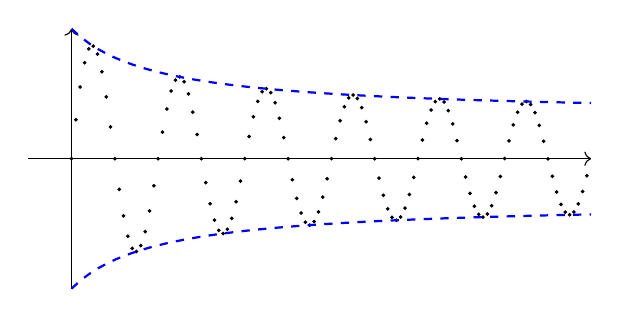
\begin{tikzpicture}[scale=1.1]
          \draw[->] (-0.5,0) -- (6,0);
          \draw[->] (0,-1.5) -- (0,1.5);
          
          % Draw the sine wave with smaller dots through exactly 5 periods
          \foreach \x in {0, 0.05, 0.1, ..., 6}
            \filldraw[black] (\x, {((1/(\x+1))+0.5)*sin(2*pi*\x r)}) circle (0.4pt); 

          \draw[blue, dashed, thick] plot[domain=0:6, samples=60] (\x, {1/(\x+1)+0.5});
          \draw[blue, dashed, thick] plot[domain=0:6, samples=60] (\x, {-1/(\x+1)-0.5});
        \end{tikzpicture}
        \caption{In order to find the limsup, we first look the whole sequence in $\mathbb{N}$ and find the supremum. We now "decrease" our domain from $\mathbb{N}$ to $\{2, \ldots\}$, then $\{3, \ldots\}$, then $\{4, \ldots\}$ and so on, continuing to label the supremum of the sequence. The limit of this sequence of supremums is the limsup.}
        \label{fig:limsupinf1}
      \end{subfigure}
      \hfill 
      \begin{subfigure}[b]{0.48\textwidth}
        \centering
        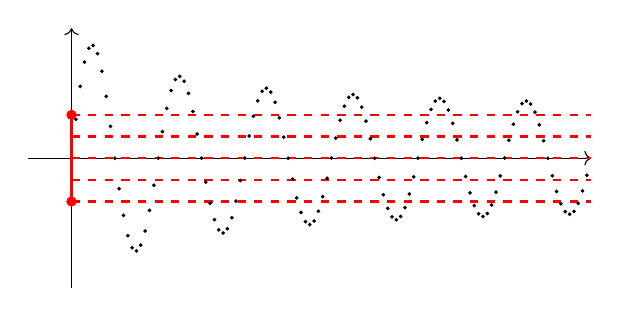
\begin{tikzpicture}[scale=1.1]
          \draw[->] (-0.5,0) -- (6,0);
          \draw[->] (0,-1.5) -- (0,1.5);
          \draw[-, red, dashed, thick] (0,0.5) -- (6,0.5);
          \draw[-, red, dashed, thick] (0,0.25) -- (6,0.25);
          \draw[-, red, dashed, thick] (0,0) -- (6,0);
          \draw[-, red, dashed, thick] (0,-0.25) -- (6,-0.25);
          \draw[-, red, dashed, thick] (0,-0.5) -- (6,-0.5);
          
          % Draw the sine wave with smaller dots through exactly 5 periods
          \foreach \x in {0, 0.05, 0.1, ..., 6}
            \filldraw[black] (\x, {((1/(\x+1))+0.5)*sin(2*pi*\x r)}) circle (0.4pt); 

          \draw[red, very thick] (0,-0.5) -- (0,0.5);
          \filldraw[red] (0,-0.5) circle (1.5pt);
          \filldraw[red] (0,0.5) circle (1.5pt);
        \end{tikzpicture}
        \caption{The 5 red lines marked in the middle (along with infinitely many others) are viable partial limits because one can choose a subsequence such that all of its points after a certain $n$ lie in some $\epsilon$-neighborhood of the limit. Therefore, we claim that the limsup/inf is the supremum of this set $E$.}
        \label{fig:limsupinf2}
      \end{subfigure}
      \caption{Two ways to visualize the superior and inferior limits of the divergent sequence $x_n = \big(\frac{1}{x+1} + 0.5\big) \sin(2\pi x)$. The left is the limit of the supremum, and the right is the supremum of the closed set of subsequential limits.} 
      \label{fig:limsupinf}
    \end{figure}
  \end{definition}

  \begin{example}[Computing Limsup and Liminf]
    We give some basic examples. 
    \begin{enumerate}
      \item Let $x_n = (-1)^n$. Then $E = \{-1, +1\}$ and 
      \begin{equation}
        \limsup_{n \rightarrow \infty} x_n = 1, \qquad \liminf_{n \rightarrow \infty} x_n = -1 
      \end{equation}

      \item Let $x_n = (-1)^n / [1 + (1/n)]$. Then 
      \begin{equation}
        \limsup_{n \rightarrow \infty} x_n = 1, \qquad \liminf_{n \rightarrow \infty} x_n = -1
      \end{equation}
    \end{enumerate}
  \end{example}

  Let's give two warnings. First, limsup and liminfs do \textit{not} behave like limits under addition and multiplication. That is, 
  \begin{equation}
    \limsup x_n + \limsup y_n \neq \limsup x_n + y_n 
  \end{equation}

  \begin{example}[Counterexamples of Arithmetic Consistency of Limit superior]
    Consider $(x_n) = (-1)^n$ and $y_n = (-1)^{n+1}$. Then 
    \begin{equation}
      \limsup x_n = \limsup y_n = 1, \qquad \liminf x_n = \liminf y_n = -1
    \end{equation}
    But $(x_n + y_n) = 0$, so 
    \begin{equation}
      \limsup x_n + y_n = \liminf x_n + y_n = 0 
    \end{equation}
  \end{example}

  Second, note that even though we are talking about subsequential limits, the limsup and liminf are \textit{not} subsequential limits! It is the supremum of subsequential limits $E$, which may or may not be in $E$. 

  \begin{example}[Limsup that is not attained by any subsequential limit]
    This should be a sequence not in $\mathbb{R}$. 
  \end{example}

  However, in $\mathbb{R}$, it turns out that the limsup and liminf are both contained in $E$, so we are fine. 

  \begin{lemma} 
    If $(x_n)$ is a sequence in $\mathbb{R}$, then 
    \begin{enumerate}
      \item the limsup is indeed a subsequential limit, i.e. $\limsup x_n \in E$. 
      \item If $x > \limsup x_n$, then $\exists N \in \mathbb{N}$ s.t. $n \geq N \implies x_n < x$. 
    \end{enumerate}
  \end{lemma}
  \begin{proof}
    For the first claim, there are two cases to consider. If $(x_n)$ is unbounded from above, then $\exists (x_{n_k})$ such that $x_{n_k} \rightarrow +\infty \implies \infty = \limsup x_n \in E$. If $(x_n)$ is bounded from above, then the subsequential limits of $(x_n)$ are either in $(x_n)$ or they are limit points of $x_n$. This implies that the set $E$ consists of points either in $\{x_n\}$ or are limit points of the set $\{x_n\} \implies \sup{E}$ is in $E$ since it's a limit point. 

    For the second claim, if there are infinitely many terms of the sequence larger than $x$, then we could find a subsequence $(x_{n_k})$ with $x_{n_k} > x$ for all $k$. Therefore $(x_n)$ has a subsequential limit which must be $\geq x$. Every subsequential limit of $(x_{n_k})$ is also a subsequential limit of $(x_n)$. This contradicts $\limsup x_n = \sup E$. 
  \end{proof}

  \begin{theorem}[Requirements of Partial Limits for Limit to Exist]
    Here are two results in which we can use partial limits to determine if a sequence has a limit or not. 
    \begin{enumerate}
      \item A sequence has a limit or tends to $\pm \infty$ if and only if its inferior and superior limits are the same. 
      \begin{equation}
        \limsup x_n = \liminf x_n = x \implies \lim_{n \rightarrow +\infty} x_n = x
      \end{equation}
      \item A sequence converges if and only if every subsequence of it converges. 
    \end{enumerate}
  \end{theorem}
  \begin{proof}
    For (1), we pick $x + \epsilon > x$. Then every term past some $N_1$ must be less than $x + \epsilon$. By the same logic, we have $N_2$ for $x - \epsilon < x$. So take $N = \max\{N_1, N_2\}$, which is contained in the $\epsilon$-ball around $x$. 
  \end{proof}

  \begin{theorem}[Ordering on Subsequential Limits]
    If $s_n \leq t_n$ for $n \geq N$, where $N$ is fixed, then 
    \begin{align*}
      \liminf_{n \rightarrow \infty} s_n & \leq \liminf_{n \rightarrow \infty} t_n \\
      \limsup_{n \rightarrow \infty} s_n & \leq \liminf_{n \rightarrow \infty} t_n 
    \end{align*}
  \end{theorem} 

  \begin{example}
    We claim 
    \begin{equation}
      \lim_{n \rightarrow \infty} n^{1/n} = 1 
    \end{equation}
    We can consider $x_n = n^{1/n} - 1$ and want to show that $x_n \rightarrow 0$. We have $x_n \geq 0$. If $n > 1$, then $n = (x_n + 1)^n \geq x_n^2 \cdot \frac{n(n - 1)}{2}$ from the binomial theorem. This means that 
    \begin{equation}
      x_n^2 \leq \frac{2}{n-1} \implies 0 \leq x_n \leq \sqrt{\frac{2}{n-1}} \rightarrow 0
    \end{equation}
    And so by the squeeze theorem, $x_n \rightarrow 0$. 
  \end{example}

  \begin{example}
    If $x > 1, \alpha \in \mathbb{R}$, then 
    \begin{equation}
      \lim_{n \rightarrow +\infty} \frac{n^\alpha}{x^n} = 0
    \end{equation} 
  \end{example}
 
\subsection{Convergence Tests for Real Series}

  \begin{definition}[Series over $\mathbb{R}$]
    Given a sequence of real numbers $(x_n)$, the \textbf{series (of partial sums)} is the sequence 
    \begin{equation}
      (s_n) = \sum_{k=1}^n x_k
    \end{equation}
    The \textbf{sum of the series} is the limit of $(s_n)$. Usually we define $(s_n)$ implicitly and use the summation notation. 
    \begin{equation}
      \sum_{n=1}^\infty x_n \coloneqq \lim_{n \rightarrow \infty} s_n
    \end{equation}
    \begin{enumerate}
      \item If the sequence $(s_n)$ converges to $s$, the series is \textbf{convergent}, written 
      \begin{equation}
        \sum x_n < +\infty
      \end{equation}
      \item If the sequence does not converge, it is \textbf{divergent}. 
      \item If the series of partial sums of $(|x_n|)$ converges, then it is said to be \textbf{absolutely convergent}.\footnote{Clearly, every absolutely convergent series because $\big|\sum_{n=1}^\infty a_n \big| \leq \sum_{n=1}^\infty |a_n|$. }
      \begin{equation}
        \sum_{n=1}^\infty |x_n|
      \end{equation}
    \end{enumerate}
  \end{definition}

  We must reiterate a few warnings here. Note that the series $\sum x_n$ is simply notation and should \textit{not} be treated as an ``infinite sum.'' Such a thing does not exist for algebraic structures which have finary operations. More specifically, given a series, we cannot in general split nor combine series, and we cannot reindex nor rearrange (an infinite number of) terms. However, we can manipulate each term for a fixed index. 

  \begin{example}[Disasters of Reindexing and Rearranging]
    Let us take the series $\sum 0$. We clearly know that the corresponding sequence of partial sums $0, 0, \ldots$ is convergent to $0$. But if we do this series of steps. 
    \begin{align}
      \sum_{n=1}^\infty 0 & = \sum_{n=1}^\infty n - n && \tag{Can manipulate terms} \\
                          & = \sum_{n=1}^\infty n - \sum_{n=1}^\infty n && \tag{Cannot split series} \\ 
                          & = 1 + \sum_{n=2}^\infty n - \sum_{n=1}^\infty n && \tag{Can take 1st term out} \\ 
                          & = 1 + \sum_{n=1}^\infty (n+1) - \sum_{n=1}^\infty n && \tag{Cannot reindexing} \\
                          & = 1 + \sum_{n=1}^\infty (n+1) - n  && \tag{Cannot combine series} \\
                          & = 1 + \sum_{n=1}^\infty 1 && \tag{Can manipulate terms} \\
                          & = 1 + \infty = +\infty
    \end{align}
    The wrong steps show that the series is divergent. 
  \end{example} 

  We have seen the consequences of these mistakes that beginners make and are often on popular media. However, note that we can always do splitting, combining, reindexing, and rearranging for \textit{finite sums}, which are algebraically defined. Later on, we will show that some of these operations are allows for series that we know are convergent.  

  Since the convergence of a series is equivalent to convergence of its sequence of partial sums, applying the Cauchy convergence criterion to the sequence $\{s_n\}$ leads to the following theorem. 

  \begin{theorem}[Cauchy Convergence Criterion for Series]
    The series $a_1 + \ldots + a_n + \ldots$ converges if and only if for every $\epsilon > 0$ there exists $N \in \mathbb{N}$ such that for all $m \geq n > N$, 
    \begin{equation}
      |a_n + \ldots + a_m| < \epsilon
    \end{equation}
  \end{theorem}

  \begin{corollary}[nth Term Test]
    A necessary (but not sufficient) condition for convergence of the series $a_1 + \ldots a_n + \ldots$ is that the terms tend to $0$ as $n \rightarrow \infty$. That is, it is necessary that
    \begin{equation}
      \lim_{n\rightarrow \infty} a_n = 0
    \end{equation}
  \end{corollary}
  \begin{proof}
    It suffices to set $m = n$ in the Cauchy convergence criterion. This would mean that for every $\epsilon > 0$ there exists a $N \in \mathbb{N}$ such that 
    \begin{equation}
      |a_n| = |a_n - 0| < \epsilon \text{ for all } n > N
    \end{equation}
    which, by definition, means that $\{a_n\}$ converges to $0$. 
  \end{proof} 

  Nothing so far is really suprising here. The Cauchy convergence criterion really just follows from the definition of Cauchy completeness, and the $n$th term test is pretty trivial. The way that we will build up convergence tests is by proving some special cases of convergence and then using the direct comparison test to then classify further series.     

  \begin{example}[Telescoping Series]
    A \textbf{telescoping series} is a series in which the partial sums can cancel out. An example is the series of partial sums of the sequence $(x_n) = \frac{1}{n (n+1)}$. In here, the series term is
    \begin{align}
      s_n & = \sum_{k=1}^n \frac{1}{k(k+1)} \\ 
          & = \sum_{k=1}^n \frac{1}{k} - \frac{1}{k+1} \\
          & = \sum_{k=1}^n \frac{1}{k} - \sum_{k=1}^n \frac{1}{k+1} \\
          & = \sum_{k=1}^n \frac{1}{k} - \sum_{k=2}^{n+1} \frac{1}{k} \\
          & = \frac{1}{1} + \bigg( \sum_{k=2}^n \frac{1}{k} \bigg) - \bigg( \sum_{k=2}^n \frac{1}{k} \bigg) - \frac{1}{n+1} \\
          & = 1 + \bigg( \sum_{k=2}^n \frac{1}{k} - \frac{1}{k} \bigg) - \frac{1}{n+1} \\
          & = 1 - \bigg( \sum_{k=2}^n 0 \bigg) - \frac{1}{n+1} \\
          & = 1 - \frac{1}{n+1} 
    \end{align} 
    Note that all of the examples that we have done here are for finite sums, so they are all legal. 
  \end{example}

  \begin{example}[Geometric Series]
    The series $\sum_{n=0}^\infty q^n$ is called a \textbf{geometric series}. 
    \begin{equation}
      1 + q + q^2 + \ldots + q^n + \ldots
    \end{equation}
    is called the \textbf{geometric series}. We can see that 
    \begin{enumerate}
      \item $|q| \geq 1 \iff \sum q^n$ is divergent. $|q| \geq 1 \implies |q|^n \geq 1$, and so the terms $q^n$ does not converge to $0$, and the $n$th term test is not met. 
      \item $|q| < 1 \iff \sum q^n$ is convergent. We can use the identity 
      \begin{equation}
        s_n = 1 + q + \ldots + q^{n-1} = \frac{1 - q^n}{1-q} \implies \lim_{n \rightarrow \infty} \frac{1 - q^n}{1 - q} = \frac{1}{1 - q}
      \end{equation} 
      since $\lim_{n\rightarrow \infty} q^n = 0$ if $|q|<1$. 
    \end{enumerate}
  \end{example}

  The Cauchy convergence criterion can be used to prove the direct comparison test. 

  \begin{theorem}[Direct Comparison Test] 
    For some fixed $N$, if 
    \begin{enumerate}
      \item If $|x_n| \leq y_n$ for all $n \geq N$ and $\sum y_n$ converges, then $\sum x_n$ converges. 
      \item If $x_n \geq y_n \geq 0$ for all $n \geq N$  and $\sum y_n$ diverges, then $\sum x_n$ diverges. 
    \end{enumerate}
  \end{theorem} 

  \begin{example}[Comparison with Telescoping Series]
    We can prove the special case a geometric series with the direct comparison test. We claim that $\sum_{n=1}^\infty \frac{1}{n^2}$ is finite. We can see that 
    \begin{equation}
      \frac{1}{n^2} \leq \frac{2}{n (n+1)} 
    \end{equation}
    where the series of the terms in the RHS is telescoping and therefore converges. So by the direct comparison test, $\sum \frac{1}{n^2}$ converges. 
  \end{example}

  Now we prove another corollary of the Cauchy convergence criterion.   

  \begin{theorem}[Cauchy Condensation Test]
    If $a_1 \geq a_2 \geq \ldots \geq 0$, the series $\sum_{n=1}^\infty a_n$ converges if and only if the series 
    \begin{equation}
      \sum_{k=0}^\infty 2^k a_{2^k} = a_1 + 2 a_2 + 4a_4 + 8a_8 + \ldots 
    \end{equation}
    converges. 
  \end{theorem}
  \begin{proof}
    Letting $A_k = a_1 + a_2 + \ldots + a_k$ and $S_n = a_1 + 2a_2 + \ldots + 2^n a_{2^n}$, it is clear that by adding up the inequalities
    \begin{align*}
      & a_2 \leq a_2 \leq a_1 \\
      & 2a_4 \leq a_3 + a_4 \leq 2a_2 \\
      & 4a_8 \leq a_5 + a_6 + a_7 + a_8 \leq 4a_4 \\
      & \ldots \\
      & 2^n a_{2^{n+1}} \leq a_{2^n + 1} + \ldots + a_{2^{n+1}} \leq 2^n a_{2^n}, 
    \end{align*}
    we get
    \begin{equation}
      \frac{1}{2}(S_{n+1} - a_1) \leq A_{2^{n+1}} - a_1 \leq S_n
    \end{equation}
    Since the sequences $\{A_k\}$ and $\{S_k\}$ are nondecreasing, and hence from the inequalities we can conclude that they are either both bounded above (which means that they are both convergent since it is a bounded, nondecreasing series) or both unbounded above (which means that they are both divergent since they are nondecreasing and unbounded). 
  \end{proof}

  \begin{corollary}[p-series Test]
    The series 
    \begin{equation}
      \sum_{n=1}^\infty \frac{1}{n^p}
    \end{equation}
    converges for $p>1$ and diverges for $p \leq 1$.\footnote{This sort of reminds you of $u$-substitution. For example, look at $\int_1^\infty f(t) \,dt = \int_0^\infty e^u f(e^u)\,du$, where the convergence of LHS $\iff$ convergence of RHS.}
  \end{corollary}
  \begin{proof}
    Suppose $p\geq 0$. By the previous theorem, the series converges or diverges simultaneously with the series 
    \begin{equation}
      \sum_{k=0}^\infty 2^k \frac{1}{(2^k)^p} = \sum_{k=0}^\infty (2^{1-p})^k
    \end{equation}
    which is really just a geometric series. A necessary and sufficient condition for the convergence of this series is that $2^{1-p} < 1$, that is, $p>1$. 

    Now suppose $p \leq 0$. The series is then clearly divergent since all of the terms are larger than $1$. 
  \end{proof}

  \begin{example}[Harmonic Series]
    The \textbf{harmonic series} 
    \begin{equation}
      1 + \frac{1}{2} + \frac{1}{3} + \ldots + \frac{1}{n} + \ldots
    \end{equation}
    seems at first glance to be converging since the terms converge to $0$. However, it does not pass the Cauchy condensation test since 
    \begin{equation}
      \sum_{n=1}^\infty 2^n x_n = \sum_{n=1}^\infty 2^n \frac{1}{2^n} = \sum_{n=1}^\infty 1 = +\infty
    \end{equation}
    As you can see, this increases logarithmically, so in early calculators it was hard to numerically detect divergence (you would have to double the number of series terms to get a linear increase). 
  \end{example} 

\subsection{Ratio and Root Tests} 

  Now we introduce the root and ratio tests, which are derived by the comparison test with a geometric series. The ratio test is used more day-to-day, but not as decisive as the root test. Both tests have a similar flavor. 

  \begin{theorem}[Ratio Test]
    Suppose the limit $\lim_{n\rightarrow \infty} \big| \frac{a_{n+1}}{a_n} \big| = \alpha$ exists for the series $\sum_{n=1}^\infty a_n$. Then, 
    \begin{enumerate}
      \item $\alpha < 1 \implies \sum a_n$ converges absolutely. 
      \item $\alpha > 1 \implies \sum a_n$ diverges.
      \item $\alpha = 1 \implies \sum a_n$ is inconclusive. 
    \end{enumerate}
    Alternatively, if 
    \begin{enumerate}
      \item $\limsup |a_{n+1}/a_n| = \alpha < 1$, then $\sum a_n$ converges 
      \item If $\exists N$ s.t. $|a_{n+1}/a_n| \geq 1$ for all $n \geq N$, then $\sum a_n$ diverges. 
    \end{enumerate}
  \end{theorem}
  \begin{proof}
    Since $\limsup \big| \frac{a_{n+1}}{a_n} \big| = \alpha < 1$, fix any $\alpha < \beta < 1$. Then $\exists N$ s.t. if $n > N$, $|a_{n+1}/a_n| < \beta$. So $|a_{N+1}| < \beta |a_N| \implies |a_{N+2}| < \beta^2 |a_N|$. So letting $C = |a_N|$, for all $m \geq N$, 
    \begin{equation}
      |a_m| \leq \frac{C}{\beta^N} \beta^m \implies |a_m| \leq \Tilde{C} \beta^m \text{ for all } m \geq N
    \end{equation}
    So $\sum a_n$ converges by comparison test since $\sum \beta^m < \infty$ when $\beta < 1$. 
  \end{proof}

  \begin{theorem}[Root Test]
    Let $\sum_{n=1}^\infty a_n$ be a given series and 
    \begin{equation}
      \alpha = \limsup_{n\rightarrow \infty} \sqrt[n]{|a_n|}
    \end{equation}
    Then, 
    \begin{enumerate}
      \item $\alpha < 1 \implies \sum a_n$ converges. 
      \item $\alpha > 1 \implies \sum a_n$ diverges. 
      \item $\alpha = 1 \implies \sum a_n$ is inconclusive. 
    \end{enumerate}
  \end{theorem} 
  \begin{proof}
    Listed. 
    \begin{enumerate}
      \item If $\limsup \sqrt[n]{|a_n|} = \alpha < 1$, take any $\alpha < \beta < 1$. Then $\exists N \in \mathbb{N}$ s.t. if $n \geq N$, then $|a_n|^{1/n} < \beta \iff |a_n| < \beta^n$. Since $\beta < 1$, $\sum \beta^n < \infty$, and by comparison test, $\sum a_n$ converges. 

      \item Suppose $\alpha > 1$. Then $\limsup |a_n|^{1/n} = \alpha > 1$. So there exists a subsequence $(a_{n_k})$ s.t. $(|a_{n_k}|^{1/n_k}) \rightarrow \alpha > 1$. This means $\exists N$ s.t. for $n \geq N$, $|a_{n_k}|^{1/{n_k}} > 1 \implies |a_{n_k}| > 1$. But this fails the $n$th term test. 

      \item We do not claim anything and so there's nothing to prove. 
    \end{enumerate}
  \end{proof}

  \begin{example}[Root Test Inconclusive Results]
    Consider $\sum \frac{1}{n} = +\infty$, but from the root test 
    \begin{equation}
      \sqrt[n]{\frac{1}{n}} \rightarrow 1, \text{ so } \alpha = 1
    \end{equation}
    Consider $\sum \frac{1}{n^2} < +\infty$, but from from the root test 
    \begin{equation}
      \sqrt[n]{\frac{1}{n^2}} = \bigg( \frac{1}{n^{1/n}} \bigg)^2 \rightarrow 1, \text{ so } \alpha = 1
    \end{equation}
  \end{example}

  \begin{example}
    The sequence $\sum \frac{c^n}{n!}$ always converges for $c \in \mathbb{R}$. 
  \end{example}

  \begin{theorem}[Weierstrass M-test for Absolute Convergence]
    Let $\sum_{n=1}^\infty a_n$ and $\sum_{n=1}^\infty b_n$ be series. Suppose there exists an index $N \in \mathbb{N}$ such that $|a_n| \leq b_n$ for all $n>N$. Then, 
    \begin{equation}
      \sum_{n=1}^\infty b_n \text{ converges } \implies \sum_{n=1}^\infty a_n \text{ converges absolutely}
    \end{equation}
  \end{theorem}

  We finally conclude by giving a theorem about the convergence of some special sequences. 

  \begin{theorem}[Special Sequences]
    Some special sequences: 
    \begin{enumerate}
      \item If $p > 0$, then $\lim_{n \rightarrow \infty} \frac{1}{n^p} = 0$. 
      
      \item If $p > 0$, then $\lim_{n \rightarrow \infty} \sqrt[n]{p} = 1$. 

      \item $\lim_{n \rightarrow \infty} \sqrt[n]{n} = 1$. 

      \item If $p > 0$ and $\alpha$ is real, then $\lim_{n \rightarrow \infty} \frac{n^\alpha}{(1 + p)^n} = 0$. 
      
      \item If $|x| < 1$, then $\lim_{n \rightarrow \infty} x^n = 0$. 
    \end{enumerate}
  \end{theorem}

\subsection{Euler's Number and Trigonometric Functions} 

  \begin{definition}[Euler's Number]
    We define \textbf{Euler's number} as 
    \begin{equation}
      e \coloneqq \sum_{n=0}^\infty \frac{1}{n!}
    \end{equation}
  \end{definition}
  
  The first thing we should do is show that it converges, this is a one-liner. 
  \begin{equation}
    \sum_{n=0}^\infty \frac{1}{n!} = 1 + 1 + \sum_{n=2}^\infty \frac{1}{n!} \leq 2 + \sum_{n=2}^\infty \frac{1}{n(n-1)} 
  \end{equation}

  \begin{theorem}[Euler's Number as a Limit]
    We have 
    \begin{equation}
      \lim_{n \rightarrow +\infty} \bigg( 1 + \frac{1}{n} \bigg)^n = e 
    \end{equation}
  \end{theorem}
  \begin{proof}
    Let us define the sequence 
    \begin{equation}
      t_n = \sum_{k=0}^n \frac{1}{k!}, \qquad s_n = \bigg( 1 + \frac{1}{n} \bigg)^n
    \end{equation}
    We know that $t_n \rightarrow e$, and we want to show that $s_n \rightarrow e$. We do this with the squeeze theorem. 
    \begin{enumerate}
      \item We can see that 
      \begin{align}
        s_n & = \bigg( 1 + \frac{1}{n} \bigg)^n \\ 
            & = \sum_{k=0}^n \binom{n}{k} 1^{n-k} \bigg( \frac{1}{n} \bigg)^k \\
            & = 1 + 1 + \frac{n(n-1)}{2!} \frac{1}{n^2} + \frac{n(n-1)(n-2)}{3!} \frac{1}{n^3} + \ldots \\ 
            & = 1 + 1 + \frac{1}{2!} (1) \bigg( 1 - \frac{1}{n} \bigg) + \frac{1}{3!} (1) \bigg(1 - \frac{1}{n} \bigg) \bigg(1 - \frac{2}{n} \bigg) + \ldots + \frac{1}{n!} (1) \prod_{k=1}^{n-1} \bigg(1 - \frac{k}{n} \bigg) \\
            & \leq \frac{1}{0!} + \frac{1}{1!} + \frac{1}{2!} + \frac{1}{3!} + \ldots + \frac{1}{n!} = t_n 
      \end{align}
      and so $s_n < t_n \implies \limsup s_n \leq \limsup t_n = e$. 

      \item Let $m \leq n$ be fixed. Then, 
      \begin{equation}
        s_n \geq 1 + 1 + \frac{1}{2!} \bigg( 1 - \frac{1}{n} \bigg) + \ldots + \frac{1}{m!} \bigg(1 - \frac{1}{n} \bigg) \bigg(1 - \frac{2}{n} \bigg) \ldots \bigg(1 - \frac{m-1}{n} \bigg) 
      \end{equation}
      since we are just taking the first $m$ positive terms of the element. Therefore, letting $n \rightarrow +\infty$ and keeping $m$ fixed, we get 
      \begin{equation}
        \liminf_{n \rightarrow +\infty} s_n \geq 1 + 1 + \frac{1}{2!} + \ldots + \frac{1}{n!} \text{ for all } m \in \mathbb{N}
      \end{equation}
      which implies $\liminf s_n \geq t_m$ for all $m \in \mathbb{N}$, and now letting $m \rightarrow +\infty$, we have $\liminf s_n \geq \liminf t_m = e$. 
    \end{enumerate}
  \end{proof}

  Now we prove the irrationality of $e$. It is usually extremely difficult to prove that an arbitrary number is irrational, e.g. $\pi^e$ or $\pi^{e^e}$. 

  \begin{theorem}[$e$ is Irrational]
    $e$ is irrational. 
  \end{theorem}
  \begin{proof} 
    Letting $t_n = \sum_{k=0}^n \frac{1}{k!}$, we have 
    \begin{align}
      e - t_n & = \sum_{k=n+1}^\infty \frac{1}{k!} \\
              & = \frac{1}{(n+1)!} \bigg( 1 + \frac{1}{n+2} + \frac{1}{(n+3)(n+2)} + \ldots \bigg) \\
              & < \frac{1}{(n+1)!} \underbrace{\bigg( 1 + \frac{1}{n+2} + \frac{1}{(n+2)^2} + \ldots \bigg)}_{\text{geometric}} \\
              & = \frac{1}{(n+1)!} \bigg( \frac{1}{1 - (1/(n+2)!)}\bigg) \\
              & = \frac{1}{n! n} \cdot \underbrace{\frac{(n+2) n}{(n+1)^2}}_{< 1} \\
              & = \frac{1}{n! n}
    \end{align}
    Note that we can combine and split sums since we know that $e$ is convergent. Now suppose that $e = p/q$. Then, 
    \begin{equation}
      0 < q! (e - t_q) < \frac{1}{q}
    \end{equation}
    But $q! e$ is an integer and $q! t_q$ is also an integer. So we have $q! \cdot \frac{p}{q}$, an integer, between $0$ and $1$, which is a contradiction. 
  \end{proof}

  Since we have defined some number $e \in \mathbb{R}$, we know that exponential exist, and therefore we the function $x \mapsto e^x$ is well-defined. In fact, it is so important that we have a separate name for it. 

  \begin{definition}[Exponential Function]
    The \textbf{exponential function} is generally referred to as the function $x \mapsto e^x$. 
  \end{definition}

  There is a nice series representation. 

  \begin{theorem}[Exponential Function as a Series]
    We have 
    \begin{equation}
      e^x = \sum_{n=0}^\infty \frac{x^n}{n!}
    \end{equation}
  \end{theorem}
  \begin{proof}
    
  \end{proof}

  Now that this is done, we can define the trigonometric functions formally as such. 

  \begin{definition}[Trigonometric Functions]
    We have 
    \begin{align}
      \sin x&=\sum_{n=0}^{\infty}\frac{(-1)^n}{(2n+1)!}x^{2n+1}=x-\frac{x^3}{3!}+\frac{x^5}{5!}-\cdots
      \\\\
      \cos x&=\sum_{n=0}^{\infty}\frac{(-1)^n}{(2n)!}x^{2n}=1-\frac{x^2}{2!}+\frac{x^4}{4!}-\cdots
    \end{align}
  \end{definition}


 
\section{Limits and Continuity of Functions} 

  We now extend our analysis to real-valued functions over a metric space. The ones that we will be particularly interested in are \textit{continuous functions}. But before this, let's introduce a new notation. Given a metric space $X$, we will talk about a variable $x$ approaching a particular value $a \in X$, denoted $x \rightarrow a$. But this isn't clear. When we talk about the concept of something approaching another thing, we have two definitions. 
  \begin{enumerate}
    \item A \textit{sequence} can approach to its limit, which is a \textit{point}. 
    \item A \textit{point} can be a limit point of a \textit{set}. 
  \end{enumerate} 
  When we write $x \rightarrow a$, we are talking about some indeterminate variable $x$ and a point $a$, it isn't immediately clear what this means. As we will soon define, this will refer to a neighborhood of $a$ or equivalently to \textit{all} sequences converging to $a$. So we can think of $x \rightarrow a$ as notation for all sequences $(x_n) \rightarrow a$.   

  \begin{definition}[Constant and Ultimately Constant Functions]
    Given a real-valued function $f: E \longrightarrow \mathbb{R}$ defined on domain $E \subset \mathbb{R}$,
    \begin{enumerate}
      \item $f$ is a \textbf{constant function} if $f(x) = A$ for all $x \in E$
      \item $f$ is called \textbf{ultimately constant} as $x \rightarrow a$ if it is constant in some deleted neighborhood $\mathring{U} (a)$, where $a$ is a limit point of $E$.
    \end{enumerate}
  \end{definition} 

  \begin{definition}[Bounded and Ultimately Bounded Functions]
    Given a real-valued function $f: E \longrightarrow \mathbb{R}$ defined on domain $E \subset \mathbb{R}$,
    \begin{enumerate}
      \item $f$ is \textbf{bounded}, \textbf{bounded above}, or \textbf{bounded below} respectively if there is a number $C \in \mathbb{R}$ such that $|f(x)|<C$, $f(x)<C$, or $C<f(x)$ for all $x \in E$.

      \item $f$ is \textbf{ultimately bounded}, \textbf{ultimately bounded above}, or \textbf{ultimately bounded below} as $x \rightarrow a$ if it is bounded, bounded above, or bounded below in some deleted neighborhood $\mathring{U}_E (a)$. 
    \end{enumerate}
  \end{definition}

  \begin{example}[Unbounded but Ultimately Bounded]
    The function 
    \begin{equation}
      f(x) = \sin{\frac{1}{x}} + x \cos{\frac{1}{x}}
    \end{equation}
    for $x \neq 0$ is not bounded on the domain of definition, but it is ultimately bounded as $x \rightarrow 0$. 
  \end{example}

\subsection{Limits of Functions}

  \begin{definition}[Limit of a Function]
    Let $f: X \rightarrow Y$ be a map between metric spaces, with $E \subset X$ and  $p \in E^\prime$ (note the limit point!). We say $f(x) \rightarrow q$ as $x \rightarrow p$, i.e. 
    \begin{equation}
      \lim_{x \rightarrow p} f(x) = q
    \end{equation} 
    if it meets the following equivalent conditions. 
    \begin{enumerate}
      \item \textit{$\epsilon$-$\delta$ Definition}. If $\forall \epsilon > 0$, $\exists \delta > 0$ s.t. $0 < d_X (x, p) < \delta \implies d_Y (f(x), q)) < \epsilon$.\footnote{Note that the strictly inequality $0 < d_X (x, p)$ is important to ensure that $x \neq p$, since functions can jump at $p$.} 

      \begin{figure}[H]
        \centering 
        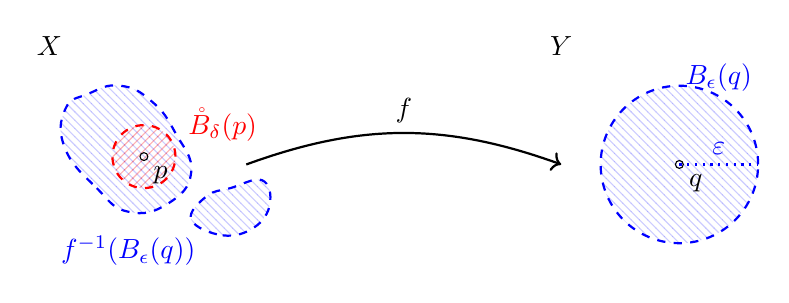
\begin{tikzpicture}
          \node at (0, 3) {$X$};
          \node at (6.5, 3) {$Y$};
          
          % Function arrow
          \draw[->, thick, bend left=20] (2.5,1.5) to node[above] {$f$} (6.5,1.5);
          
          % Blue blob 1 - made bigger but still in top left
          \draw[blue, thick, dashed] plot [smooth cycle, tension=0.8] coordinates {(0.2,1.7) (0.6,1.2) (1.0,0.9) (1.5,1.0) (1.8,1.4) (1.6,1.9) (1.3,2.3) (0.9,2.5) (0.5,2.4) (0.2,2.2)};
          \fill[blue, pattern=north west lines, pattern color=blue, opacity=0.2] plot [smooth cycle, tension=0.8] coordinates {(0.2,1.7) (0.6,1.2) (1.0,0.9) (1.5,1.0) (1.8,1.4) (1.6,1.9) (1.3,2.3) (0.9,2.5) (0.5,2.4) (0.2,2.2)};
          \node at (1.0,0.4) [blue] {$f^{-1}(B_\epsilon(q))$};
          
          % Blue blob 2 - in bottom right
          \draw[blue, thick, dashed] plot [smooth cycle, tension=0.7] coordinates {(1.8,0.8) (2.2,0.6) (2.6,0.7) (2.8,1.0) (2.7,1.3) (2.3,1.2) (2.0,1.1)};
          \fill[blue, pattern=north west lines, pattern color=blue, opacity=0.2] plot [smooth cycle, tension=0.7] coordinates {(1.8,0.8) (2.2,0.6) (2.6,0.7) (2.8,1.0) (2.7,1.3) (2.3,1.2) (2.0,1.1)};
          
          % Left neighborhood (red, hatched circle) - moved inside V1
          \draw[red, thick, dashed] (1.2,1.6) circle (0.4);
          \fill[red, pattern=north east lines, pattern color=red, opacity=0.3] (1.2,1.6) circle (0.4);
          \node at (2.2,2) [red] {$\mathring{B}_\delta(p)$};
          
          % Point p - hollow and red - also moved
          \draw (1.2,1.6) circle (0.05);
          \node at (1.2,1.6) [below right] {$p$};
          
          % Right neighborhood (blue circle)
          \draw[blue, thick, dashed] (8,1.5) circle (1);
          \fill[blue, pattern=north west lines, pattern color=blue, opacity=0.2] (8,1.5) circle (1);
          \node at (8.5,2.6) [blue] {$B_\epsilon(q)$};
          
          % Point q - where f(p) would be, now just a point reference
          \draw (8,1.5) circle (0.05);
          \node at (8,1.5) [below right] {$q$};
          
          % Epsilon visualization - dotted line segment not touching the blue boundary
          \draw[blue, thick, dotted] (8,1.5) -- (9,1.5) node[midway, above] {$\varepsilon$};
        \end{tikzpicture}
        \caption{Said in one line, the preimage of any open ball around $y = f(x)$ must contain some open deleted open ball around $x$.} 
        \label{fig:limit_function}
      \end{figure}

      \item \textit{Sequential Definition}. If for all sequences $(x_n) \rightarrow p$, $f(x_n) \rightarrow q$.

      \begin{figure}[H]
        \centering 
        \begin{tikzpicture}[scale=1]
          % Space labels without axes
          \node at (1, 3) {$X$};
          \node at (7.5, 3) {$Y$};
          
          % Function arrow
          \draw[->, thick, bend left=20] (3.5,1.5) to node[above] {$f$} (7.5,1.5);
          
          % Point a in domain - shifted by 1
          \fill (2.5,1.5) circle (0.07);
          \node at (2.5,1.5) [above right] {$p$};
          
          % Blue sequence (x_n) in domain - curved path - shifted by 1
          \filldraw[blue] (1.3,0.6) circle (0.03);
          \filldraw[blue] (1.7,0.8) circle (0.03);
          \filldraw[blue] (1.9,1.0) circle (0.03);
          \filldraw[blue] (2.1,1.3) circle (0.03);
          \filldraw[blue] (2.3,1.4) circle (0.03);
          \node at (1.6,0.4) [blue] {$(x_n)$};
          
          % Red sequence (y_n) in domain - curved path - shifted by 1
          \filldraw[red] (2.7,1.6) circle (0.03);
          \filldraw[red] (2.9,1.7) circle (0.03);
          \filldraw[red] (3.0,1.8) circle (0.03);
          \filldraw[red] (3.2,1.85) circle (0.03);
          \filldraw[red] (3.5,1.9) circle (0.03);
          \node at (3.4,2.0) [red] {$(y_n)$};
          
          % Point A in codomain
          \fill (8,1.5) circle (0.07);
          \node at (8,1.5) [above right] {$q$};
          
          % Blue sequence (f(x_n)) in codomain - curved path
          \filldraw[blue] (7.1,0.7) circle (0.03);
          \filldraw[blue] (7.3,0.9) circle (0.03);
          \filldraw[blue] (7.5,1.1) circle (0.03);
          \filldraw[blue] (7.7,1.2) circle (0.03);
          \filldraw[blue] (7.8,1.4) circle (0.03);
          \node at (7.2,0.4) [blue] {$(f(x_n))$};
          
          % Red sequence (f(y_n)) in codomain - curved path
          \filldraw[red] (8.2,1.7) circle (0.03);
          \filldraw[red] (8.5,1.8) circle (0.03);
          \filldraw[red] (8.7,2.0) circle (0.03);
          \filldraw[red] (8.9,2.3) circle (0.03);
          \filldraw[red] (9.1,2.5) circle (0.03);
          \node at (9.2,1.9) [red] {$(f(y_n))$};
        \end{tikzpicture}
        \caption{For every sequence that converges to the left, the new sequence mapped through $f$ converges to $q$. Note that we choose the points $x_n$ to be in the "deleted" neighborhood $E\setminus a$ (neighborhood $E$ with point $a$ removed) to force us to choose a sequence that is not $a, a, \ldots$. That is, it forces us to choose different points for the sequence. } 
        \label{fig:sequential_limit_def}
      \end{figure}
    \end{enumerate}
  \end{definition}
  \begin{proof}
    We prove equivalence. 
    \begin{enumerate}
      \item $(\rightarrow)$. Assume $\lim_{x \rightarrow p} f(x) = q$. Let $(x_n) \in E$ s.t. $x_n \rightarrow p$ with $x_n \neq p$. We wish to show that $f(x_n) \rightarrow q$. Let $\epsilon > 0$. Then $\exists \delta > 0$ s.t. $0 < d_X (x, p) < \delta \implies d_Y (f(x), q) < \epsilon$. Since $\delta > 0$, by definition $\exists N \in \mathbb{N}$ s.t. if $n \geq N$, $d_X (x_n , p) < \delta \implies d_Y (f(x_n), q)$. 
    \end{enumerate}
  \end{proof}

  Sometimes, the $\epsilon$-$\delta$ definition is good, but a lot of the times the sequential definition is good enough and more insightful. 

  \begin{example}[Limit of the Signum Function]
    The function sgn$: \mathbb{R} \longrightarrow \mathbb{R}$ defined
    \begin{equation}
      \text{sgn}\,x = \begin{cases} 1, & x > 0 \\ 0, & x = 0 \\ -1, & x < 0 \end{cases}
    \end{equation}
    has no limit as $x \rightarrow 0$. 

    First, it is ludicrous that the limit would be any number that is not $\{-1, 0, 1\}$. If we assume that $A \not\in \{-1,0,1\}$, then we can choose any arbitrarily small $\epsilon$-neighborhood of $A$ that does not include the three numbers. Clearly, there doesn't exist any $\delta>0$ such that the deleted $\delta$-neighborhood of $0$ maps to a set completely contained in the $\epsilon$-neighborhood of $A$. That is,
    \begin{equation}
      \text{sgn}\big( \mathring{U}_\delta (0)\big) = \{-1,1\} \not\subset U_\epsilon (A)
    \end{equation}
    It doesn't even intersect the $\epsilon$-neighborhood at all. 
    \begin{enumerate}
      \item If $A = 1$, we can construct a $\epsilon$-neighborhood $V_A$ for $\epsilon = \frac{1}{2}$. Clearly, there exists no open neighborhood $U_0$ of $0$ that is entirely mapped to $V$, since $U_0$ contains both negative numbers and $0$ and hence must be mapped to $0, -1$. 
      \item Similarly, given the $(\epsilon=\frac{1}{2})$-neighborhood of $A = -1$, there exists no open neighborhood $U_0$ of $0$ that is entirely mapped to it, since $U_0$ contains both positive numbers and $0$ and hence must be mapped to $0, 1$. 
      \item Finally, given the $(\epsilon=\frac{1}{2})$-neighborhood of $A = 0$, there exists no open neighborhood $U_0$ of $0$ that is entirely mapped to it, since $U_0$ contains both positive and negative numbers and hence must be mapped to $\pm1$. 
    \end{enumerate}
    Therefore, the limit does not exist. 
  \end{example}

  \begin{example}[Limit of Absolute Value of Signum Function]
    We will show that 
    \begin{equation}
      \lim_{x \rightarrow 0} |\text{sgn}\,x| = 1
    \end{equation}
    We construct a $\epsilon$-neighborhood $U_\epsilon (1)$ around $1$. Given this neighborhood, we can imagine choosing the deleted $\delta$-neighborhood $\mathring{U}_\delta (0)$ around $0$. Since every element in $\mathring{U}_\delta (0)$ maps to $1$, it is clearly in $U_\epsilon$. In fact, for arbitrarily small $\epsilon > 0$, we can choose \textbf{any} $\delta>0$ since everything in $\mathbb{R} \setminus 0$ maps to $1$. We can visualize this in $\mathbb{R}^2$ as
  \end{example}

  \begin{theorem}[Arithmetic on Limits of Functions]
    Given two numerical valued functions $f, g: E \subset \mathbb{R} \longrightarrow \mathbb{R}$ with a common domain where $g(x) \neq 0$ for all $x \in E$, let 
    \begin{equation}
      \lim_{x \rightarrow a} f(x) = A, \;\;\;\;\; \lim_{x \rightarrow a} g(x) = B
    \end{equation}
    then, 
    \begin{align*}
      & \lim_{x \rightarrow a} (f+g)(x) = A + B \\
      & \lim_{x \rightarrow a} (cf)(x) = cA \\
      & \lim_{x \rightarrow a} (f \cdot g)(x) = A \cdot B \\
      & \lim_{x \rightarrow a} \bigg(\frac{f}{g}\bigg) (x) = \frac{A}{B}
    \end{align*}
  \end{theorem}
  \begin{proof}
    Cauchy sequence criterion for a limit immediately proves this. 
  \end{proof}

  We end this with a theorem connecting the relationship between a limit of a function as $x \rightarrow a$ and its ultimate behavior as $x \rightarrow a$. 

  \begin{theorem}
    Let $f: E \longrightarrow \mathbb{R}$ be a function. Then, 
    \begin{enumerate}
      \item $f$ is ultimately the constant $A$ as $x \rightarrow a$ implies that $\lim_{x \rightarrow a} f(x) = A$. 
      \item $\lim_{x \rightarrow a} f(x)$ implies that $f$ is ultimately bounded as $x \rightarrow a$. 
    \end{enumerate}
  \end{theorem}

  \begin{definition}[Infinitesimal Function]
    A function $f: E \subset \mathbb{R} \longrightarrow \mathbb{R}$ is said to be \textbf{infinitesimal} as $x \rightarrow a$ if 
    \[\lim_{x \rightarrow a} f(x) = 0\]
  \end{definition}

  \begin{lemma}[Sums, Products of Infinitesimals]
    It is clear that if $\alpha, \beta$ are infinitesimal as $x \rightarrow a$, then 
    \begin{enumerate}
      \item $\alpha + \beta$ is infinitesimal as $x \rightarrow a$
      \item $\alpha \cdot \beta$ is infinitesimal as $x \rightarrow a$
    \end{enumerate}
    Furthermore, if $\alpha$ is infinitesimal and $\beta$ is ultimately bounded as $x \rightarrow a$, then the product $\alpha \cdot \beta$ is infinitesimal as $x \rightarrow a$. 
  \end{lemma}
  \begin{proof}
  We prove all three statements. 
  \begin{enumerate}
    \item Assume that $\alpha$ and $\beta$ are infinitesimal as $x \rightarrow a$. Then, let us fix a small $\epsilon>0$. This means that for every $\frac{\epsilon}{2}$ there exists an open deleted neighborhood $\mathring{U}^\prime (a)$ such that its image $\alpha\big(\mathring{U}^\prime (a)\big)\subset U^\prime_{\epsilon/2} (0) \subset \mathbb{R}$. Additionally, for every $\frac{\epsilon}{2}$ there exists an open deleted neighborhood $\mathring{U}^{\prime\prime} (a)$ such that its image $\beta\big(\mathring{U}^{\prime\prime} (a)\big)\subset U^\prime_{\epsilon/2} (0) \subset \mathbb{R}$.
    Thus, for the deleted neighborhood 
    \[\mathring{U}(a) \subset \mathring{U}^\prime (a) \cup \mathring{U}^{\prime\prime} (a)\]
    we can see that for all $x \in \mathring{U}(a)$, 
    \[|(\alpha + \beta)(x)| = |\alpha (x) + \beta(x)| \leq |\alpha (x)| + |\beta(x)| < \frac{\epsilon}{2} + \frac{\epsilon}{2} = \epsilon\]
    and hence $(\alpha + \beta)\big( \mathring{U}(a)\big) \subset U_\epsilon (0)$. 
    \item This case is a special case of assertion 3. That is, every function that has a limit is ultimately bounded. 
    \item Since $\beta(x)$ is ultimately bounded, this means that there exists a constant $M$ and an open deleted neighborhood $\mathring{U}^\prime (a) \subset E$ such that for all $x \in \mathring{U}^\prime (a)$, its image is bounded: $|\beta(x)|<M$. Let us fix a small $\epsilon>0$. Then, by definition of the limit, for every $\frac{\epsilon}{M}$ there exists an open deleted neighborhood $\mathring{U}^{\prime\prime} (a)$ such that its image $\beta\big(\mathring{U}^{\prime\prime}(a)\big) \subset U_{\epsilon/M} (0) \subset \mathbb{R}$. Therefore, for the deleted neighborhood
    \[\mathring{U}(a) \subset \mathring{U}^\prime (a) \cup \mathring{U}^{\prime\prime}(a)\]
    we can see that for all $x \in \mathring{U} (a)$, 
    \[|(\alpha \cdot \beta)(x)| = |\alpha (x) \beta(x)| = |\alpha (x)| |\beta(x)| < \frac{\epsilon}{M} \cdot M = \epsilon\]
    Therefore, $(\alpha \cdot \beta)\big( \mathring{U} (a)\big) \subset U_\epsilon (0)$. 
  \end{enumerate}
  \end{proof}

  Note that in proving these properties of the limits, we have used the following fact about open deleted neighborhoods around $a$. 
  \begin{enumerate}
    \item $\mathring{U} (a)$ is not the empty set. 
    \item Given open deleted neighborhoods $\mathring{U}^\prime (a)$ and $\mathring{U}^{\prime\prime} (a)$, there exists an open deleted neighborhood in the intersections of these neighborhoods. 
    \[\mathring{U} (a) \subset \mathring{U}^\prime (a) \cup \mathring{U}^{\prime\prime} (a)\]
  \end{enumerate}

  \begin{theorem}[Representation of a Convergent Function as a Shift of its Infinitesimal]
    Given a function $f: E \subset \mathbb{R} \longrightarrow \mathbb{R}$, its limit exists and 
    \begin{equation}
      \lim_{x \rightarrow a} f(x) = A
    \end{equation}
    if and only if $f$ can be represented as 
    \begin{equation}
      f(x) = A + \alpha (x)
    \end{equation}
    where $\alpha$ is infinitesimal as $x \rightarrow a$. We can visualize this theorem by thinking of a function $f$ that results from a "shift" of an infinitesimal. 

    \begin{figure}[H]
      \centering 
      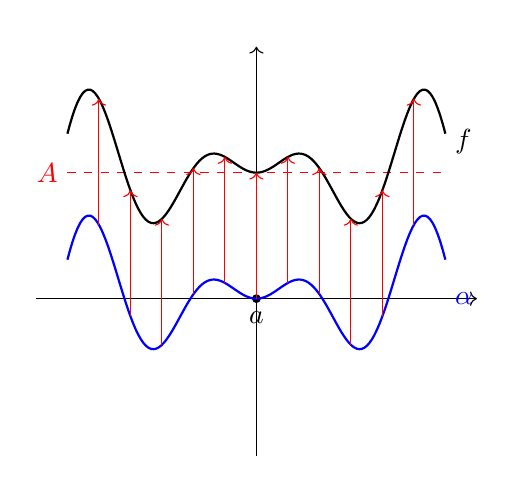
\begin{tikzpicture}[scale=0.8]
          % Coordinate axes
          \draw[->] (-3.5,0) -- (3.5,0) node[right] {};
          \draw[->] (0,-2.5) -- (0,4) node[above] {};
          
          % Point a on x-axis
          \node at (0,-0.3) {$a$};
          \fill (0,0) circle (0.07);
          
          % Blue function (alpha): x*sin(x)
          \draw[blue, thick, domain=-3:3, samples=150] 
            plot (\x, {0.5*\x*sin(3*\x r)});
          
          % Blue alpha label without arrow
          \node[blue, right] at (3,0) {$\alpha$};
          
          % Red horizontal line for A
          \draw[red, dashed] (-3,2) -- (3,2);
          \node[red, left] at (-3,2) {$A$};
          
          % Black function (f): x*sin(x) + 2
          \draw[black, thick, domain=-3:3, samples=150] 
            plot (\x, {0.5*\x*sin(3*\x r) + 2});
          
          % Black f label without arrow
          \node[black, right] at (3,2.5) {$f$};
          
          % Red vertical arrows connecting blue function to red line
          \foreach \x in {-2.5, -2.0, -1.5, -1.0, -0.5, 0, 0.5, 1.0, 1.5, 2.0, 2.5}
          \draw[->, red] (\x, {0.5*\x*sin(3*\x r)}) -- (\x, {0.5*\x*sin(3*\x r) + 2});
      \end{tikzpicture}
      \caption{Shift of $f(x) = \frac{1}{2} x \sin(3x) + 2$.} 
      \label{fig:infinitesimal_shift_function}
    \end{figure}
  \end{theorem}

  Finally, we reiterate some limit theorems already stated for sequences, but now corresponding to functions. Interpreting the function limit as the Cauchy sequence definition of limits renders the proofs of these theorems trivial. 

  \begin{theorem}[Bounds on Limits of Functions]
    If the functions $f, g: E \rightarrow \mathbb{R}$ are such that
    \begin{equation}
      \lim_{x\rightarrow a} f(x) = A < B = \lim_{x \rightarrow a} g(x)
    \end{equation}
    then there exists a deleted neighborhood $U_\delta (a)$ in $E$ at each point of which $f(x) < g(x)$. 
  \end{theorem}

  \begin{theorem}[Squeeze Theorem for Limits of Functions]
    Given the functions $f, g, h: E \subset \mathbb{R} \longrightarrow \mathbb{R}$ such that
    \begin{equation}
      f(x) \leq g(x) \leq h(x) \text{ for all } x \in E
    \end{equation}
    then, 
    \begin{equation}
      \lim_{x \rightarrow a} f(x) = \lim_{x \rightarrow a} h(x) = C \implies \lim_{x \rightarrow a} g(x) = C
    \end{equation}
  \end{theorem}

\subsection{Asymptotic Behavior of Functions}

    \begin{definition}[Little-O Notation]
      The function $f: E \longrightarrow \mathbb{R}$ is said to be \textbf{infinitesimal compared with the function $g: E \longrightarrow \mathbb{R}$} as $x \rightarrow a$, written (by abuse of notation) $f = o(g)$ as $x \rightarrow a$, if 
      \[\lim_{x \rightarrow a} \frac{f(x)}{g(x)} = 1\]
      or in other words, if $f/g$ is an infinitesimal function as $x \rightarrow a$. Therefore, $f = o(1)$ as $x \rightarrow a$ means that $f$ is infinitesimal as $x \rightarrow a$. \footnote{Note that writing $f = o(g)$ is again, an abuse of notation. $f = o(g)$ is really a shorthand way of writing that $f$ is in the class of functions that is infinitesimal compared with the function $g$.}
    \end{definition}

    Intuitively, $f = o(g)$ means that the ratio between $f(x)$ and $g(x)$ will tend to infinity as $x \rightarrow a$ (this does not mean that $f$ will be infinitely greater than $g$, however!). 

    \begin{example}[Linear vs Quadratic]
      For example, looking at the two functions $f(x) = x^2$ and $g(x) = x$, we have 
      \begin{enumerate}
        \item $x^2 = o(x)$ as $x \rightarrow 0$ (since $\frac{x^2}{x} = x$ is infinitesimal as $x \rightarrow 0$)
        \item $x = o(x^2)$ as $x \rightarrow \infty$ (since $\frac{x}{x^2} = \frac{1}{x}$ is infinitesimal as $x \rightarrow \infty$)
      \end{enumerate}
      We can visualize $g/f (x)$ tending to infinity within a neighborhood of $0$ and $f/g (x)$ tending to infinity within a neighborhood of $\infty$. 
      
      \begin{figure}[H]
        \centering 
        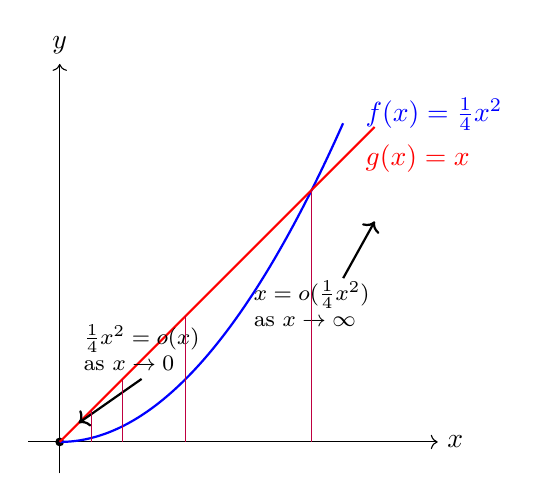
\begin{tikzpicture}[scale=0.8]
            % Coordinate axes
            \draw[->] (-0.5,0) -- (6,0) node[right] {$x$};
            \draw[->] (0,-0.5) -- (0,6) node[above] {$y$};
            
            % Origin point
            \fill (0,0) circle (0.07);
            
            % Blue parabola: f(x) = 1/4 * x^2
            \draw[blue, thick, domain=0:4.5, samples=100] 
              plot (\x, {0.25*\x*\x});
            
            % Red linear function: g(x) = x
            \draw[red, thick, domain=0:5, samples=2] 
              plot (\x, {\x});
            
            % Function labels
            \node[blue, right] at (4.7,5.2) {$f(x)=\frac{1}{4}x^2$};
            \node[red, right] at (4.7,4.5) {$g(x)=x$};
            
            % Asymptotic behavior annotations
            \node[align=left, font=\footnotesize] at (1.3,1.5) {$\frac{1}{4}x^2=o(x)$\\as $x\to 0$};
            \draw[->, thick] (1.3,1) -- (0.3,0.3);
            
            \node[align=left, font=\footnotesize] at (4,2.2) {$x=o(\frac{1}{4}x^2)$\\as $x\to\infty$};
            \draw[->, thick] (4.5,2.6) -- (5,3.5);
            
            % Vertical comparison lines
            \draw[purple, thin] (0.5,0) -- (0.5,0.5);
            \draw[purple, thin] (0.5,0) -- (0.5,0.0625);
            
            \draw[purple, thin] (1,0) -- (1,1);
            \draw[purple, thin] (1,0) -- (1,0.25);
            
            \draw[purple, thin] (2,0) -- (2,2);
            \draw[purple, thin] (2,0) -- (2,1);
            
            \draw[purple, thin] (4,0) -- (4,4);
            \draw[purple, thin] (4,0) -- (4,4);
        \end{tikzpicture}
        \caption{} 
        \label{fig:quadratic_vs_linear}
      \end{figure}
    \end{example}

    \begin{definition}[Orders of Infinitesimals, Infinities]
      If $f = o(g)$ and $g$ is infinitesimal as $x \rightarrow a$, then $f$ is an \textbf{infinitesimal of higher order than $g$ as $x \rightarrow a$}. Furthermore, if $f$ and $g$ are infinite functions as $x\rightarrow a$ and $f = o(g)$ as $x \rightarrow a$, then $g$ is a \textbf{higher order infinity than $f$ as $x \rightarrow a$}. 
    \end{definition}

    \begin{definition}[Big-O Notation]
      By abuse of notation, $f = O(g)$ as $x \rightarrow a$ means that 
      \begin{equation}
        \lim_{x \rightarrow a} \frac{f(x)}{g(x)} = \infty
      \end{equation}
      or in other words, $f/g$ is ultimately bounded as $x \rightarrow a$. In particular, $f = O(1)$ as $x \rightarrow a$ means that $f$ is bounded within a certain neighborhood $U(a)$ of $a$. 
    \end{definition}

    \begin{definition}[Functions of Same Order]
      The functions $f$ and $g$ are of the same over as $x \rightarrow a$, written 
      \begin{equation}
        f \asymp g \text{ as } x \rightarrow a
      \end{equation}
      if $f = O(g)$ and $g = O(f)$ as $x \rightarrow a$. Intuitively, this means that the ratio between $f$ and $g$ within some deleted neighborhood of $a$ is finite. 

      Note that the condition that $f$ and $g$ be of the same order as $x \rightarrow a$ is (by definition of ultimately bounded functions) equivalent to the condition that there exist $c_1, c_2 > 0$ and an open neighborhood $U (a)$ such that the relations
      \begin{equation}
        c_1 |g(x)| \leq |f(x)| \leq c_2 |g(x)|
      \end{equation}
      is true for $x \in U(a)$. 
    \end{definition}

    \begin{definition}[Asymptotic Equivalence of Functions]
      For functions $f$ and $g$, if 
      \begin{equation}
        \lim_{x \rightarrow a} \frac{f(x)}{g(x)} = 1
      \end{equation}
      we say that \textbf{$f$ behaves asymptotically like $g$ as $x \rightarrow a$}, or that \textbf{$f$ is equivalent to $g$ as $x \rightarrow a$}, written 
      \begin{equation}
        f \sim g \text{ as } x \rightarrow a
      \end{equation}
      Moreover, $\sim$ is an equivalence relation, which means that
      \begin{enumerate}
        \item $f \sim f$ as $x \rightarrow a$
        \item $f \sim g$ as $x \rightarrow a \implies$ $g \sim f$ as $x \rightarrow a$
        \item $f \sim g$ and $g \sim h$ as $x \rightarrow a \implies f \sim h$ as $x \rightarrow a$
      \end{enumerate}
    \end{definition}

    We list a few examples in order to develop some sort of visual intuition for when two functions are asymptotically equivalent. 

    \begin{example}[Both Converges at Finite Value to Nonzero Finite Value]
      If $f(a) = g(a) \neq 0$, then $f \sim g$ trivially since the ratio of $f$ and $g$ converges to $1$ within a neighborhood of $a$. 

      \begin{figure}[H]
        \centering 
        \begin{tikzpicture}[scale=1.2]
          % Coordinate axes
          \draw[->] (-3,0) -- (3,0) node[right] {$x$};
          \draw[->] (0,-1) -- (0,3) node[above] {$y$};
          
          % Blue curve - single smooth wave with no other intersections
          \draw[blue, thick, smooth] 
            plot[domain=-3:3, samples=50] (\x, {1.5 + 0.8*sin(\x*40)});
          
          % Red curve - continuous rise with no other intersections
          \draw[red, thick, smooth] 
            plot[domain=-2:3, samples=50] (\x, {0.2*\x*\x - 0.6*\x + 1});
          
          % Point of intersection
          \fill (-0.4,1.25) circle (0.05);
          \node[above] at (-0.4,1.25) {$a$};
        \end{tikzpicture}
        \caption{} 
      \end{figure}
    \end{example}

    \begin{example}[Both Converges at Finite Value to $0$]
      When $f(a) = g(a) = 0$, it may be $f$ may be equivalent to $g$ or one function may be infinitesimally smaller than the other. 

      \begin{figure}[H]
        \centering
        \begin{subfigure}[b]{0.48\textwidth}
          \centering
          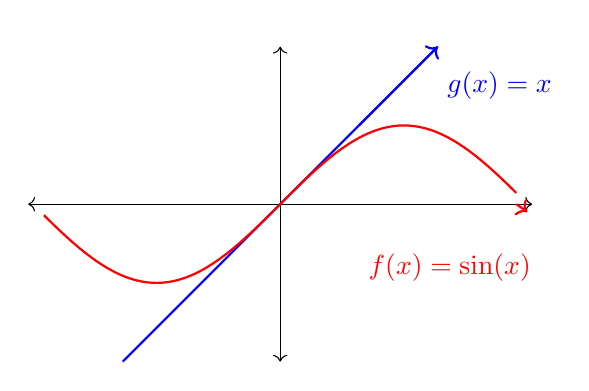
\begin{tikzpicture}[scale=1.0]
            % Coordinate axes
            \draw[<->] (-3.2,0) -- (3.2,0) node[right] {};
            \draw[<->] (0,-2) -- (0,2) node[above] {};
            
            % Blue line g(x) = x with restricted domain
            \draw[blue, thick] (-2,-2) -- (2,2);
            \node[blue, right] at (2,1.5) {$g(x)=x$};
            
            % Red sine curve f(x) = sin(x)
            \draw[red, thick, domain=-3:3, samples=100] 
              plot (\x, {sin(\x r)});
            \node[red, right] at (1,-0.8) {$f(x)=\sin(x)$};
            
            % Direction arrows
            \draw[blue, ->, thick] (1,1) -- (2,2);
            \draw[red, ->, thick] (3,0) -- (3.14,-0.1);
          \end{tikzpicture}
          \caption{When $f(x) = \sin{x}$ and $g(x) = x$, then $f \sim g$ since we see that $\lim_{x \rightarrow 0} \frac{\sin{x}}{x} = 1$, and so $\sin{x} \sim x$ as $x \rightarrow 1$. }
        \end{subfigure}
        \hfill 
        \begin{subfigure}[b]{0.48\textwidth}
          \centering
          \begin{tikzpicture}[scale=0.8]
            % Coordinate axes
            \draw[<->] (-3.5,0) -- (3.5,0) node[right] {};
            \draw[<->] (0,-3) -- (0,3) node[above] {};
            
            % Red parabola f(x) = x^2
            \draw[red, thick, domain=-2.5:2.5, samples=50] 
              plot (\x, {\x*\x*0.2});
            \node[red, right] at (2.5,2.5) {$f(x)=x^2$};
            
            % Blue cubic g(x) = x^3
            \draw[blue, thick, domain=-2.3:2.3, samples=50] 
              plot (\x, {\x*\x*\x*0.2});
            \node[blue, right] at (2.5,2) {$g(x)=x^3$};
          \end{tikzpicture}
          \caption{When $f(x) = x^2$ and $g(x) = x^3$, then $\lim_{x \rightarrow 0} \frac{x^3}{x^2} = 0$, and so $x^3 \not\sim x^2$. In fact, $x^3 = o(x^2)$. }
        \end{subfigure}

        \begin{subfigure}[b]{0.48\textwidth}
          \centering
          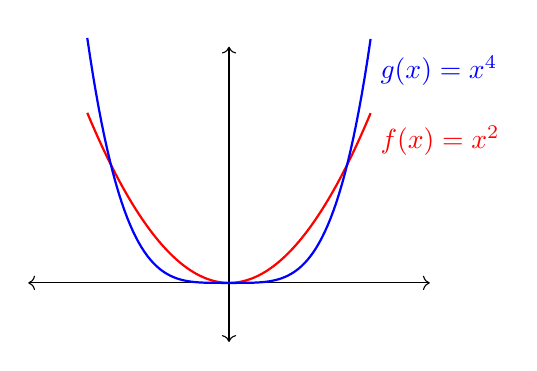
\begin{tikzpicture}[scale=1.5]
            % Coordinate axes
            \draw[<->] (-1.7,0) -- (1.7,0) node[right] {};
            \draw[<->] (0,-0.5) -- (0,2) node[above] {};
            
            % Red parabola f(x) = x^2
            \draw[red, thick, domain=-1.2:1.2, samples=100] 
              plot (\x, {\x*\x});
            \node[red, right] at (1.2,1.2) {$f(x)=x^2$};
            
            % Blue g(x) = x^4
            \draw[blue, thick, domain=-1.2:1.2, samples=100] 
              plot (\x, {\x*\x*\x*\x});
            \node[blue, right] at (1.2,1.8) {$g(x)=x^4$};
          \end{tikzpicture}
          \caption{When $f(x) = x^2$ and $g(x) = x^4$, then  $\lim_{x \rightarrow 0} \frac{x^4}{x^2} = 0$, and so $x^4 \not\sim x^2$. In fact, $x^4 = o(x^2)$. }
        \end{subfigure}
        \hfill 
        \begin{subfigure}[b]{0.48\textwidth}
          \centering
          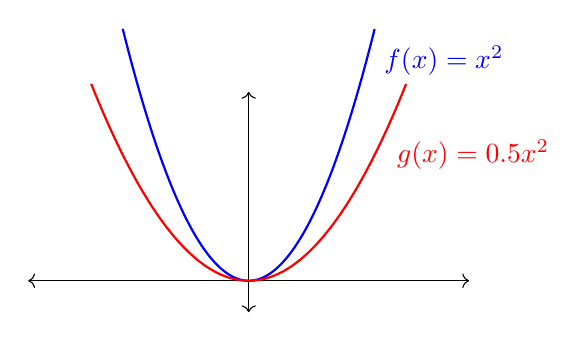
\begin{tikzpicture}[scale=0.8]
            % Coordinate axes
            \draw[<->] (-3.5,0) -- (3.5,0) node[right] {};
            \draw[<->] (0,-0.5) -- (0,3) node[above] {};
            
            % Blue parabola f(x) = x^2
            \draw[blue, thick, domain=-2:2, samples=100] 
              plot (\x, {\x*\x});
            \node[blue, right] at (2,3.5) {$f(x)=x^2$};
            
            % Red parabola g(x) = 0.5x^2
            \draw[red, thick, domain=-2.5:2.5, samples=100] 
              plot (\x, {0.5*\x*\x});
            \node[red, right] at (2.2,2) {$g(x)=0.5x^2$};
          \end{tikzpicture}
          \caption{When $f(x), g(x) = x^2, 0.5x^2$, then $\lim_{x \rightarrow 0} \frac{0.5x^2}{x^2} = \frac{1}{2}$. So $0.5x^2 \not\sim x^2$. }
        \end{subfigure}
        \caption{Examples of different scenarios.}
        \label{fig:converge_to_finite_value_0}
      \end{figure}
    \end{example}

    \begin{example}[Analyzing at Infinity]
      When analyzing the behavior of functions as $x \rightarrow \infty$, we can picture the two graphs of $f$ and $g$ on the plane and "zoom out" to see if the ratio of the values converge to $1$. This would mean that as $x \rightarrow \infty$, we should see the graphs overlapping more and more. 

      \begin{figure}[H]
        \centering
        \begin{subfigure}[b]{0.48\textwidth}
          \centering
          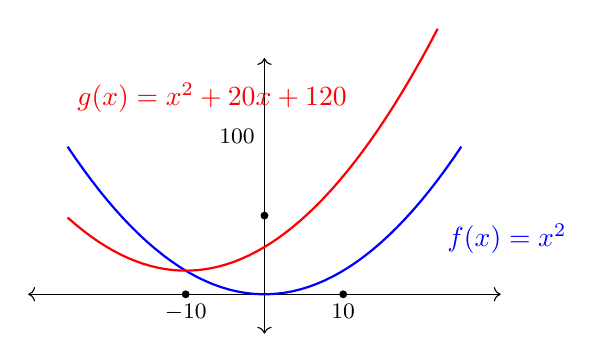
\begin{tikzpicture}[scale=1]
              % Coordinate axes
              \draw[<->] (-3,0) -- (3,0) node[right] {};
              \draw[<->] (0,-0.5) -- (0,3) node[above] {};
              
              % Blue parabola f(x) = x^2
              \draw[blue, thick, domain=-2.5:2.5, samples=50] 
                plot (\x, {0.3 * \x*\x});
              \node[blue, right] at (2.2,0.7) {$f(x)=x^2$};
              
              % Red parabola g(x) = x^2 + 10x + 100
              \draw[red, thick, domain=-2.5:2.2, samples=50] 
                plot (\x, {0.3 * (\x*\x + 2*\x + 2)});
              \node[red, right] at (-2.5,2.5) {$g(x)=x^2+20x+120$};
              
              % Key points on x-axis with labels
              \fill (-1,0) circle (0.05);
              \node[below, font=\footnotesize] at (-1,0) {$-10$};
              
              \fill (1,0) circle (0.05);
              \node[below, font=\footnotesize] at (1,0) {$10$};
              
              \fill (0,1) circle (0.05);
              \node[left, font=\footnotesize] at (0,2) {$100$};
          \end{tikzpicture}
          \caption{Comparison of $f(x)=x^2$ and $g(x)=x^2+10x+100$}
          \label{fig:shifted-quadratic}
        \end{subfigure}
        \hfill 
        \begin{subfigure}[b]{0.48\textwidth}
          \centering
          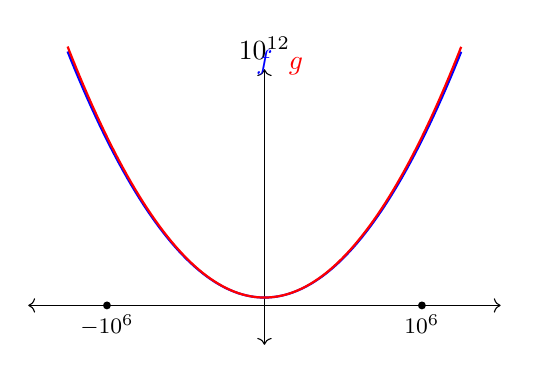
\begin{tikzpicture}[scale=1]
              % Coordinate axes
              \draw[<->] (-3,0) -- (3,0) node[right] {};
              \draw[<->] (0,-0.5) -- (0,3) node[above] {$10^{12}$};
              
              % Functions with nearly identical behavior
              \draw[blue, thick, domain=-2.5:2.5, samples=100] 
                plot (\x, {0.1 + 0.5*\x*\x});
              \node[blue, above] at (0,2.8) {$f$};
              
              % Red function slightly above blue
              \draw[red, thick, domain=-2.5:2.5, samples=100] 
                plot (\x, {0.1 + 0.51*\x*\x});
              \node[red, above] at (0.4,2.8) {$g$};
              
              % Key points on x-axis with labels
              \fill (-2,0) circle (0.05);
              \node[below, font=\footnotesize] at (-2,0) {$-10^6$};
              
              \fill (2,0) circle (0.05);
              \node[below, font=\footnotesize] at (2,0) {$10^6$};
          \end{tikzpicture}
          \caption{Asymptotic behavior with $g/f \approx 1$}
          \label{fig:asymptotic}
        \end{subfigure}
        \caption{taking $f(x) = x^2$ and $g(x) = x^2 + 10x + 100$, we can see that the discrepancy is high around a neighborhood of $x = 0$. But as $x \rightarrow +\infty$, we get $\lim_{x \rightarrow + \infty} \frac{x^2 + 10x + 100}{x^2} = 1$, and so the graphs look like they are overlapping. Notice that even though the absolute difference $|(x^2 + 10x + 100) - x^2| = |10x + 100|$ tends to infinity, this difference increases infinitesimally compared to $f$ and $g$. }
        \label{fig:function-ratios}
      \end{figure}
    \end{example}

    From this, we can see that if $f \sim g$ as $x \rightarrow a$, then their difference 
    \begin{equation}
      f - g = o(g) = o(f)
    \end{equation}
    That is, $(f-g)(x)$ is infinitesimal compared to $g$ or $f$ (doesn't matter which one we compare it to). This leads to our next section, where we formalize this concept with absolute and relative errors. 

  \subsubsection{Approximations of Functions}

    It is useful to note that since the relation $\lim_{x \rightarrow a} \gamma(x) = 1$ is equivalent to 
    \begin{equation}
      \gamma (x) = 1 + \alpha(x), \text{ where } \lim_{x \rightarrow a} \alpha(x) = 0
    \end{equation}
    the relation $f \sim g$ as $x\rightarrow a$ is equivalent to saying that
    \begin{equation}
      \frac{f(x)}{g(x)} = \gamma(x), \text{ where } \lim_{x \rightarrow a} \gamma(x) = 1
    \end{equation}
    which implies 
    \begin{equation}
      f(x) = g(x) + \alpha(x) g(x) = g(x) + o(g(x)) \text{ as } x \rightarrow a
    \end{equation}
    or, symmetrically, 
    \begin{equation}
      g(x) = f(x) + \alpha(x) f(x) = f(x) + o(f(x)) \text{ as } x \rightarrow a
    \end{equation}
    This means that $f$ can be exactly represented by another function $g$, plus another (error) function $o(g(x))$ that is infinitesimal compared to $g$. 

    \begin{figure}[H]
      \centering
      \begin{subfigure}[b]{0.48\textwidth}
        \centering
        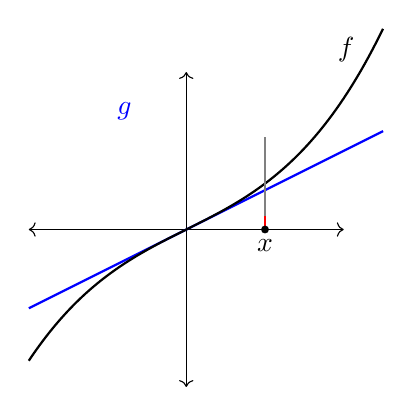
\begin{tikzpicture}[scale=1]
            % Coordinate axes
            \draw[<->] (-2,0) -- (2,0) node[right] {};
            \draw[<->] (0,-2) -- (0,2) node[above] {};
            
            % Blue line g(x) = x
            \draw[blue, thick, domain=-2:2.5, samples=2] 
              plot (\x, {\x * 0.5});
            \node[blue, right] at (-1,1.5) {$g$};
            
            % Black cubic f(x) = x^3/6 + x
            \draw[black, thick, domain=-2:2.5, samples=100] 
              plot (\x, {((\x*\x*\x)/6 + \x) * 0.5});
            \node[black, above right] at (1.8,2) {$f$};
            
            % Vertical line at a point
            \draw[gray, thin] (1,0) -- (1,1);
            \draw[gray, thin] (1,1) -- (1,1.17);
            \draw[red, thin] (1,0) -- (1,0.17);
            
            % Point label
            \fill (1,0) circle (0.05);
            \node[below] at (1,0) {$x$};
        \end{tikzpicture}
        \caption{Functions $f$, $g$, and their difference}
        \label{fig:function-diff}
      \end{subfigure}
      \hfill 
      \begin{subfigure}[b]{0.48\textwidth}
        \centering
        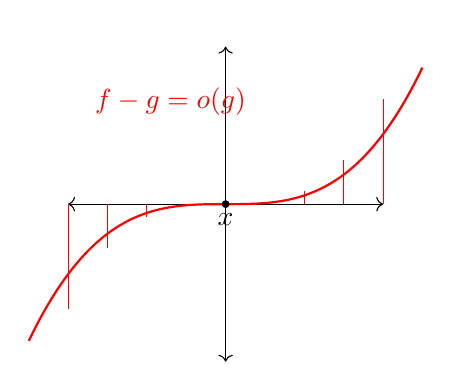
\begin{tikzpicture}[scale=1]
            % Coordinate axes
            \draw[<->] (-2,0) -- (2,0) node[right] {};
            \draw[<->] (0,-2) -- (0,2) node[above] {};
            
            % Red function f-g = x^3/6
            \draw[red, thick, domain=-2.5:2.5, samples=100] 
              plot (\x, {(\x*\x*\x)/9});
            \node[red, above] at (-0.7,1) {$f-g = o(g)$};
            
            % Vertical lines showing difference
            \foreach \x in {-2, -1.5, -1, -0.5, 0.5, 1, 1.5, 2} {
                \draw[red, thin] (\x,0) -- (\x,{(\x*\x*\x)/6});
            }
            
            % Point at origin
            \fill (0,0) circle (0.05);
            \node[below] at (0,0) {$x$};
        \end{tikzpicture}
        \caption{Behavior of $f-g$ (little-o of $g$)}
        \label{fig:little-o}
      \end{subfigure}
      \caption{Visualization of asymptotic behavior where $f-g = o(g)$}
      \label{fig:asymptotic-behavior}
    \end{figure}

    Note that it is not a sufficient condition that the error function be infinitesimal! The error function $f-g$ must be infinitesimal \textit{compared to $g$}! This tells us that not only does the error function decrease infinitesimally, but also is infinitesimal compared to the approximation function we already have, which is in general a much stronger claim. This representation of certain types functions will provide the foundation for differential calculus when we talk about "good" approximations for a function. 


    \begin{definition}[Relative Error]
      Since $f \sim g$ as $x \rightarrow a$ means that 
      \begin{equation}
        f(x) = g(x) + \alpha(x) g(x) = g(x) + o(g(x))
      \end{equation}
      we can define the \textbf{relative error} of $g$ as an approximation of $f$ to be
      \begin{equation}
        |\alpha(x)| = \bigg| \frac{f(x) - g(x)}{g(x)} \bigg|
      \end{equation}
      Clearly, since $f \sim g$, the relative error must be infinitesimal as $x \rightarrow a$. 
    \end{definition}

    We use the following lemma to check whether two functions are asymptotically equivalent. 
    \begin{lemma}
      $f \sim g$ as $x \rightarrow a$ if and only if the relative error of $g$ is infinitesimal as $x \rightarrow a$. 
    \end{lemma}

    \begin{example}
      We claim that 
      \begin{equation}
        x^2 + x = \bigg(1 + \frac{1}{x} \bigg) x^2 \sim x^2 \text{ as } x \rightarrow \infty
      \end{equation}
      We see that the absolute error of this approximation $|(x^2 + x) - x^2| = |x|$ tends to infinity, but the relative error $\frac{|x|}{x^2} = \frac{1}{|x|} \rightarrow 0$ as $x \rightarrow \infty$. 
    \end{example}

    \begin{theorem}[Prime Number Theorem]
      Let $\pi(x)$ be the number of prime numbers strictly less than $x$. Then $\pi \sim \frac{x}{\ln{x}}$ as $x\rightarrow + \infty$, or more precisely, 
      \begin{equation}
        \pi(x) = \frac{x}{\ln{x}} + o \bigg( \frac{x}{\ln{x}}\bigg) \text{ as } x \rightarrow +\infty
      \end{equation}
    \end{theorem}

    \begin{example}
      It is a fact that $\lim_{x\rightarrow 0} \frac{sin{x}}{x} = 1$, so we have $\sin{x} \sim x$ as $x \rightarrow 0$. So,
      \begin{equation}
        \sin{x} = x + o(x) \text{ as } x \rightarrow 0
      \end{equation}
    \end{example}

    The following theorem proves useful when computing limits. 

    \begin{theorem}
      If $f \sim \Tilde{f}$ as $x \rightarrow a$, then 
      \begin{equation}
        \lim_{x \rightarrow a} f(x) g(x) = \lim_{x \rightarrow a} \Tilde{f}(x) g(x)
      \end{equation}
      provided one of these limits exist. 
    \end{theorem}

    \begin{theorem}[Properties of $o(g)$ and $O(g)$ Functions]
      For $x \rightarrow a$, 
      \begin{enumerate}
        \item $o(f) + o(f) = o(f)$
        \item $o(f)$ is also $O(f)$
        \item $o(f) + O(f) = O(f)$
        \item $O(f) + O(f) = O(f)$
        \item If $g(x) \not\equiv 0$, then 
        \begin{equation}
          \frac{o(f(x))}{g(x)} = o \bigg( \frac{f(x)}{g(x)} \bigg), \text{ and } \frac{O(f(x))}{g(x)} = O \bigg( \frac{f(x)}{g(x)} \bigg)
        \end{equation}
      \end{enumerate}
    \end{theorem}

\subsection{Continuous Functions}

  \begin{definition}[Continuity of a Function]
    A function $f$ is \textbf{continuous at point $a$} if for any neighborhood $V\big(f(a)\big)$ of $f(a)$, there is a neighborhood $U(a)$ of $a$ whose image under the mapping $f$ is contained in $V\big( f(a)\big)$. 

    Generalizing this, we say that a function is \textbf{(globally) continuous} if the preimage of every neighborhood in its codomain is an open set in its domain. 
  \end{definition}

  \begin{lemma}[Existence of Limits of Continuous Functions]
    $f: E \longrightarrow \mathbb{R}$ is continuous at $a \in E$, where $a$ is a limit point of $E$ if and only if 
    \begin{equation}
      \lim_{x \rightarrow a} f(x) = f(a)
    \end{equation}
  \end{lemma}
  \begin{proof}
    The limit equaling $f(a)$ means that, by definition, for any arbitrarily small deleted neighborhood of $f(a)$, denoted $U_{f(a)} \setminus f(a)$, its preimage will be an open neighborhood of $a$, which itself will contain an open set. 
  \end{proof}

  This also means that we can use the Cauchy limit definition to defined continuity of a function at a point. That is, for any sequence $\{a_n\}$ of point in codomain $E$ which converges to point $a$, the function $f$ is continuous at $a$ if the corresponding sequence $\{f(a_n)\}$ converges to $f(a)$.

  \begin{theorem}
    This means that the continuous functions commute with the operation of passing to the limit at a point. 
    \begin{equation}
      \lim_{x \rightarrow a} f(x) = f\Big( \lim_{x \rightarrow a} x \Big)
    \end{equation}
  \end{theorem}

  \begin{lemma}[Properties of Continuous Functions]
    Let $f: \mathbb{R}^n \longrightarrow \mathbb{R}^m, \; g: \mathbb{R}^m \longrightarrow \mathbb{R}^p$ with $c \in \mathbb{R}$. 
    \begin{enumerate}
      \item $f$ continuous at $x_0 \implies$ $c f$ continous at $x_0$. 
      \item $f, g$ continuous at $x_0 \implies f + g$ continuous at $x_0$. 
      \item Let $m = 1$. $f, g$ continuous at $x_0 \implies f g$ continuous at $x_0$. 
      \item $f$ continuous at $x_0$ and $f(x) \neq 0 \forall x \in \mathbb{R}^n \implies 1 / f$ continuous at $x_0$. 
      \item If $f(x) = \big( f_1(x), f_2(x), ..., f_n(x) \big)$ coordinate-wise, then 
      \begin{equation}
        f \text{ continuous at } x_0 \iff f_1, f_2, ..., f_m \text{ continuous  at } x_0
      \end{equation}
      \item $f$ continuous at $x_0$ and $g$ continuous at $y_0 = f(x_0) \implies g \circ f$ continuous at $x_0$. 
    \end{enumerate}
  \end{lemma}
  \begin{proof}
    This is an immediate result of the equivalence of a function being continuous at point $a$ and its limit at point $a$ existing. 
  \end{proof}

  \begin{theorem}[Local Properties of Continuous Functions]
    Let $f: E \longrightarrow \mathbb{R}$ be a function that is continuous at the point $a \in E$. Then, 
    \begin{enumerate}
      \item $f$ is bounded in some neighborhood $U(a)$. 
      \item If $f(a) \neq 0$, then in some neighborhood $U(a)$ all the values of the function have the same sign as $f(a)$. 
      \item If the function $g: U(a) \subset E \longrightarrow \mathbb{R}$ is defined in some neighborhood of $a$ and is continuous at $a$, then the following functions 
      \begin{align*}
        & (f + g) (x) \\
        & (f \cdot g) (x) \\
        & \bigg( \frac{f}{g} \bigg) \big( x \big) \text{ where } g(a) \neq 0
      \end{align*}
      are also defined in $U(a)$ and continuous at $a$. 
      \item If the function $g: Y \longrightarrow \mathbb{R}$ is continuous at a point $b \in Y$ and $f$ is such that $f: E \longrightarrow Y$, $f(a) = b$, and $f$ is continuous at $a$, then the composite function 
      \[g \circ f: E \longrightarrow \mathbb{R}\]
      is defined on $E$ and continuous at $a$. This is easy to see because given the open neighborhood of $g(b)$, we know for a fact that $U_\delta (a)$ maps completely into $U_\epsilon (b)$, and that $U_\epsilon (b)$ maps completely into $U_\kappa (g(b))$ and so the composition of these mappings must mean that $U_\delta (a)$ maps completely into $U_\kappa (g(b))$. 
    \end{enumerate}
  \end{theorem}

  \begin{example}
    An algebraic polynomial 
    \begin{equation}
      P(x) = a_0 x^n + a_1 x^{n-1} + a_2 x^{n-2} + \ldots + a_{n-1} x + a_n
    \end{equation}
    is a continuous function on $\mathbb{R}$. Since $f(x) = x$ and $f(x) = c$ are continuous functions, by induction on $x$, we can multiply them together to find that $f(x) = x^n$ is continuous, which implies that $a x^n$ is continuous, which implies that the sums of these functions are also continuous. 
  \end{example}

  \subsubsection{Intermediate and Extreme Value Theorem}

    Unlike local properties, the global property of a function is a property involving the entire domain of definition of the function. 

    \begin{theorem}[Intermediate Value Theorem]
      If a function that is continuous on a closed interval assumes values with different signs at the endpoints of the interval, then there is a point in the interval where it assumes the value $0$. 
      \begin{center}
          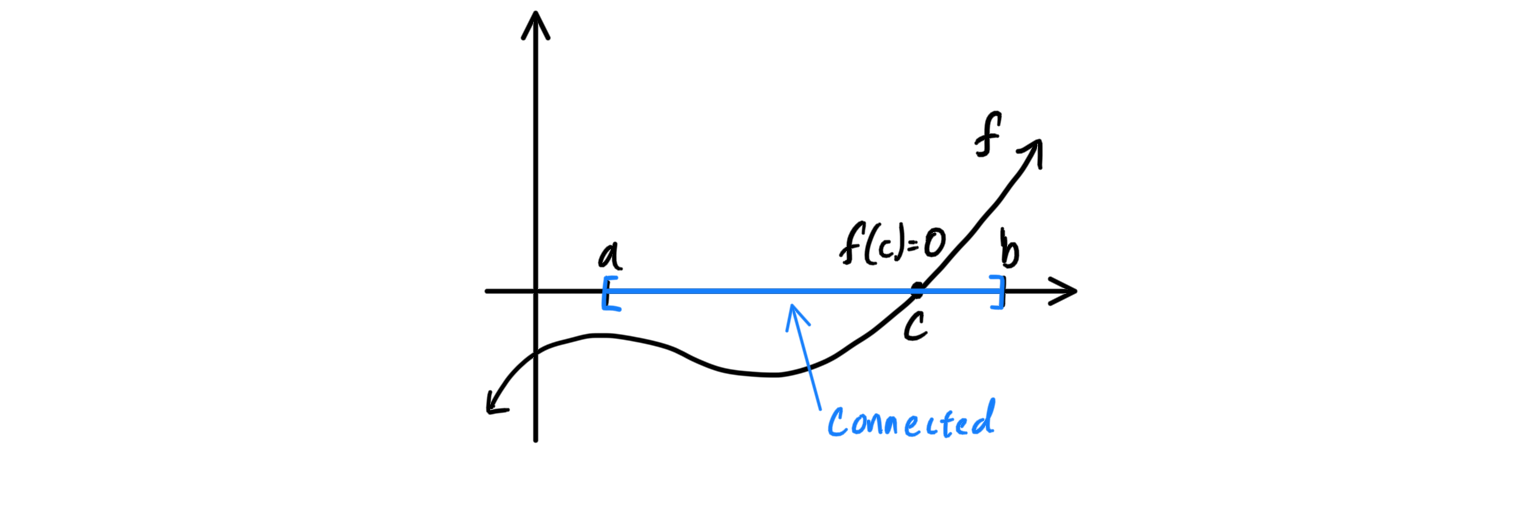
\includegraphics[scale=0.25]{img/IVT.PNG}
      \end{center}
    \end{theorem}
    \begin{proof}

    \end{proof}

    This following proof provides a very simple algorithm for finding the zero of the equation $f(x) = 0$ on an interval whose endpoints has values with opposite signs. 
    Note that the colloquial description of the intermediate value theorem, that is is impossible to pass continuously from positive to negative values without assuming the value $0$ along the way), assumes more than they state. That is, this theorem is actually dependent on the domain of definition: that is is a closed interval, or more generally, that it is \textbf{connected}. 

    \begin{corollary}
      If a function $f$ is continuous on an open interval and assumes values $f(a) = A, f(b) = B$, then for any number $C \in (A, B)$, there is a point $c$ between $a$ and $b$ such that $f(c) = C$. 
      \begin{center}
        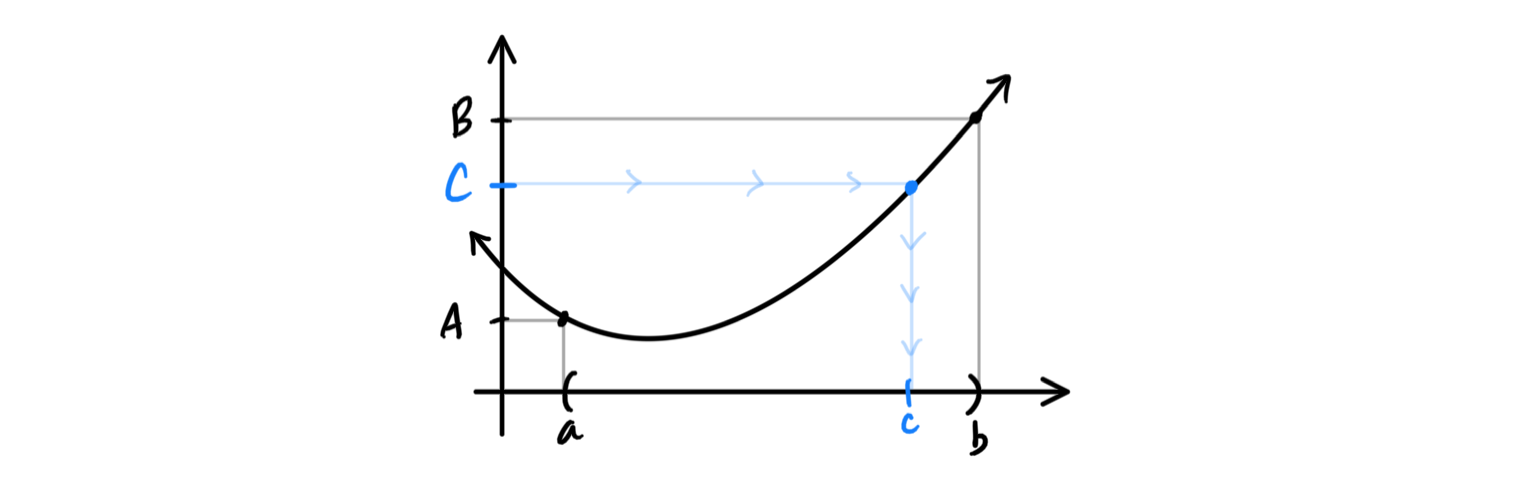
\includegraphics[scale=0.25]{img/Corollary_of_IVT.PNG}
      \end{center}
    \end{corollary}

    \begin{theorem}[Extreme Value Theorem]
      A continuous real-valued function over a compact set attains its maximum and minimum. 
    \end{theorem}

  \subsubsection{Inverse Function Theorem}

    We begin by introducing this intuitive lemma. 
    \begin{lemma}
      A continuous mapping $f: E \longrightarrow \mathbb{R}$ of a closed interval $E = [a,b]$ into $\mathbb{R}$ is injective if and only if the function $f$ is strictly monotonic on $[a,b]$. 

      Furthermore, every strictly monotonic function $f: X \subset \mathbb{R} \longrightarrow \mathbb{R}$ (for arbitrary $X$) has an inverse 
      \[f^{-1}: f(X) \subset \mathbb{R} \longrightarrow \mathbb{R}\]
      with the same kind of monotonicity on $f(X)$ that $f$ has on $X$. 
    \end{lemma}

    \begin{lemma}[Criterion for Continuity of a Monotonic Function]
      A monotonic function $f: E \longrightarrow \mathbb{R}$ defined on a closed interval $E = [a,b]$ is continuous if and only if its set of values $f(E)$ is the closed interval with endpoints $f(a)$ and $f(b)$. 

      Note that both conditions imply that there are no points of discontinuities in the graph of $f$. 
    \end{lemma}


    \begin{theorem}[Inverse Function Theorem]
    A function $f: X \longrightarrow \mathbb{R}$ that is strictly monotonic on a set $X \subset \mathbb{R}$ has an inverse $f^{-1}: Y \longrightarrow \mathbb{R}$ defined on the set $Y = f(X)$ of values of $f$. The function $f^{-1}: Y \longrightarrow \mathbb{R}$ is monotonic and has the same type of monotonicity on $Y$ that $f$ has on $X$. 
    \begin{center}
        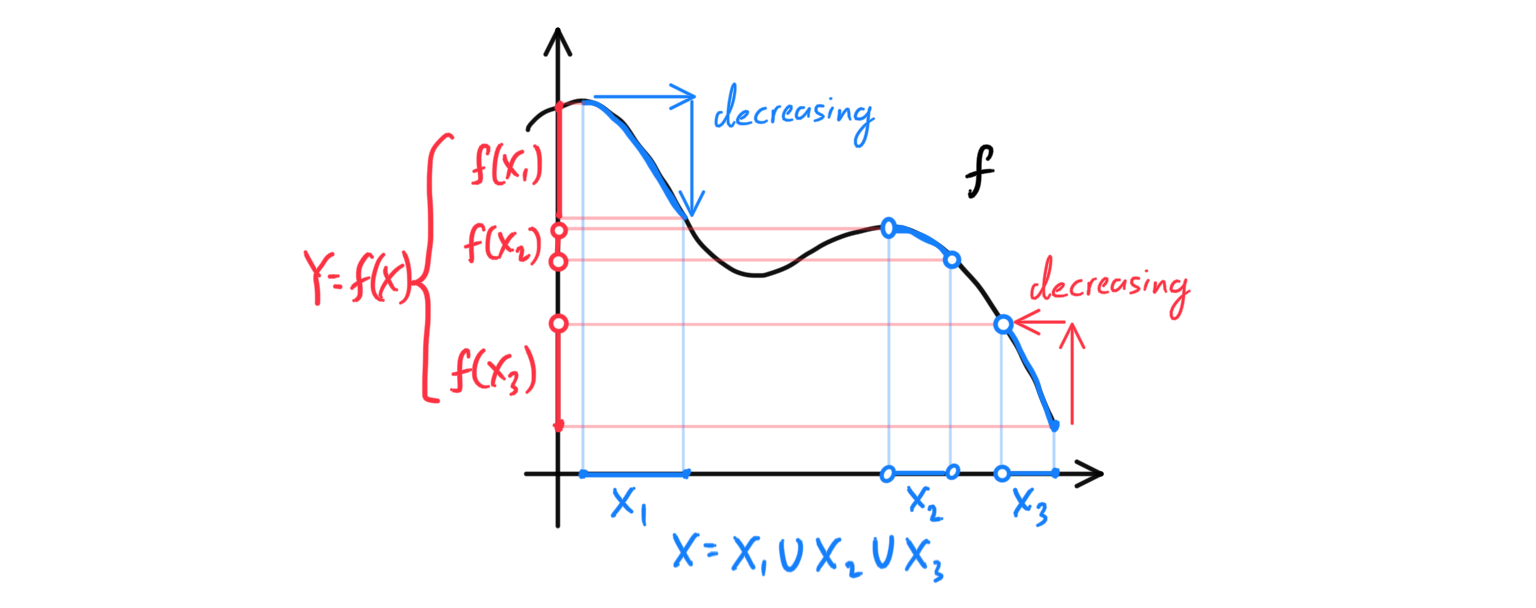
\includegraphics[scale=0.25]{img/Inverse_Function_Theorem_Analysis.PNG}
    \end{center}
    If in addition, $X$ is a closed interval $[a,b]$ and $f$ is continuous on $X$, then the set $Y = f(X)$ is the closed interval with endpoints $f(a)$ and $f(b)$ and the function $f^{-1}: Y \longrightarrow \mathbb{R}$ is continuous on it.
    \end{theorem}

    \begin{example}
      The function $f(x) = \sin{x}$ is increasing and continuous on the closed interval $\big[ -\frac{\pi}{2}, \frac{\pi}{2} \big]$. Hence, the restriction to the closed interval $\big[ -\frac{\pi}{2}, \frac{\pi}{2} \big]$ has an inverse $x = f^{-1}(y)$, which is denoted by 
      \[x = \arcsin{y}\]
      This function is defined on the closed interval $\big[- \sin\big(-\frac{\pi}{2}\big), \sin\big(-\frac{\pi}{2}\big) \big] = [-1,1]$ and increases continuously from $-\frac{\pi}{2}$ to $\frac{\pi}{2}$. 
      \begin{center}
          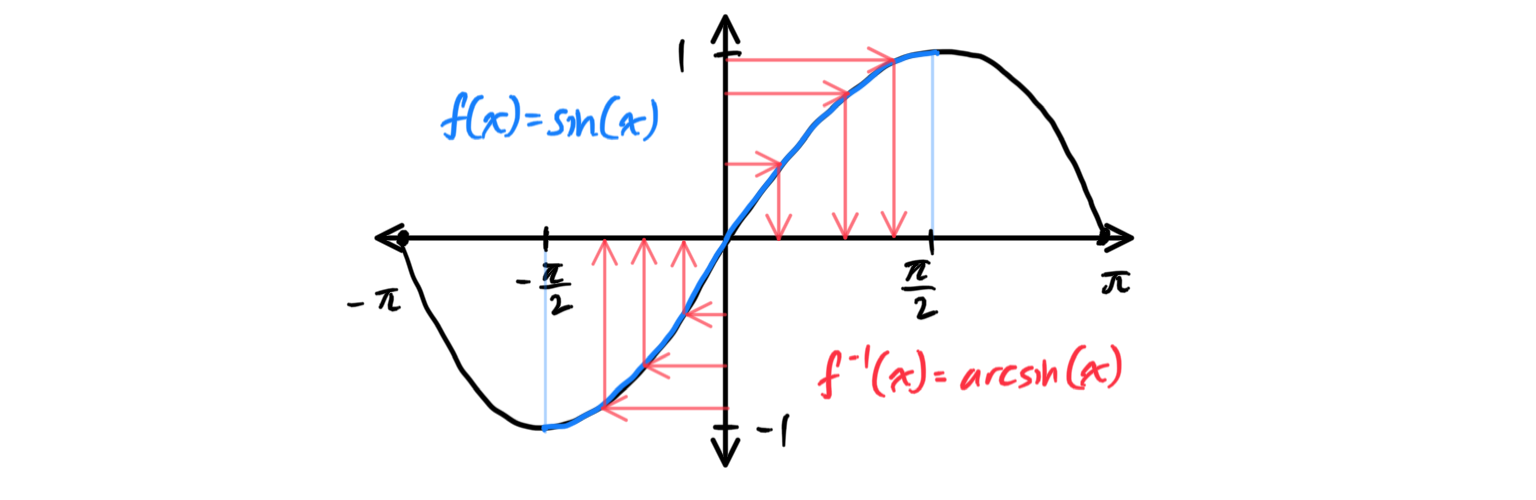
\includegraphics[scale=0.25]{img/Inverse_Function_Theorem_Sin.PNG}
      \end{center}
    \end{example}

\subsection{Uniform Continuity}

  Roughly speaking, a function $f$ is uniformly continuous if it is possible to guarantee that $f(x)$ and $f(y)$ be as close to each other as we please by requiring only that $x$ and $y$ be sufficiently close to each other. 

  \begin{definition}[Uniform Continuity]
    A function $f: E \longrightarrow \mathbb{R}$ is \textbf{uniformly continuous} on a set $E \subset \mathbb{R}$ if for every $\epsilon > 0$, there exists $\delta > 0$ such that 
    \begin{equation}
      \big| f(x_1) - f(x_2)\big| < \epsilon
    \end{equation}
    for all points $x_1, x_2 \in E$ such that $|x_1 - x_2| < \delta$. 

    Intuitively, uniform continuity says that given any two points $x, y$ in the domain where their distance is arbitrarily small ($\delta$ apart), we can guarantee that the distance between $f(x), f(y)$ is at maximum some arbitrarily small $\epsilon$. 

    The following visual shows the radical function $f(x) = \sqrt{x}$ defined on $\mathbb{R}^+$. We can see that it satisfies uniform continuity because the graph does not escape the top and/or bottom of the $\epsilon \times \delta$ window, no matter where the box is located on the graph. More strictly speaking, no matter what we set the $\epsilon$ (how long the box is), uniform continuity says that we can choose a sufficient $\delta$ (width of the box) such that the graph does not escape the top/bottom of the window no matter where the window is. 
    \begin{center}
        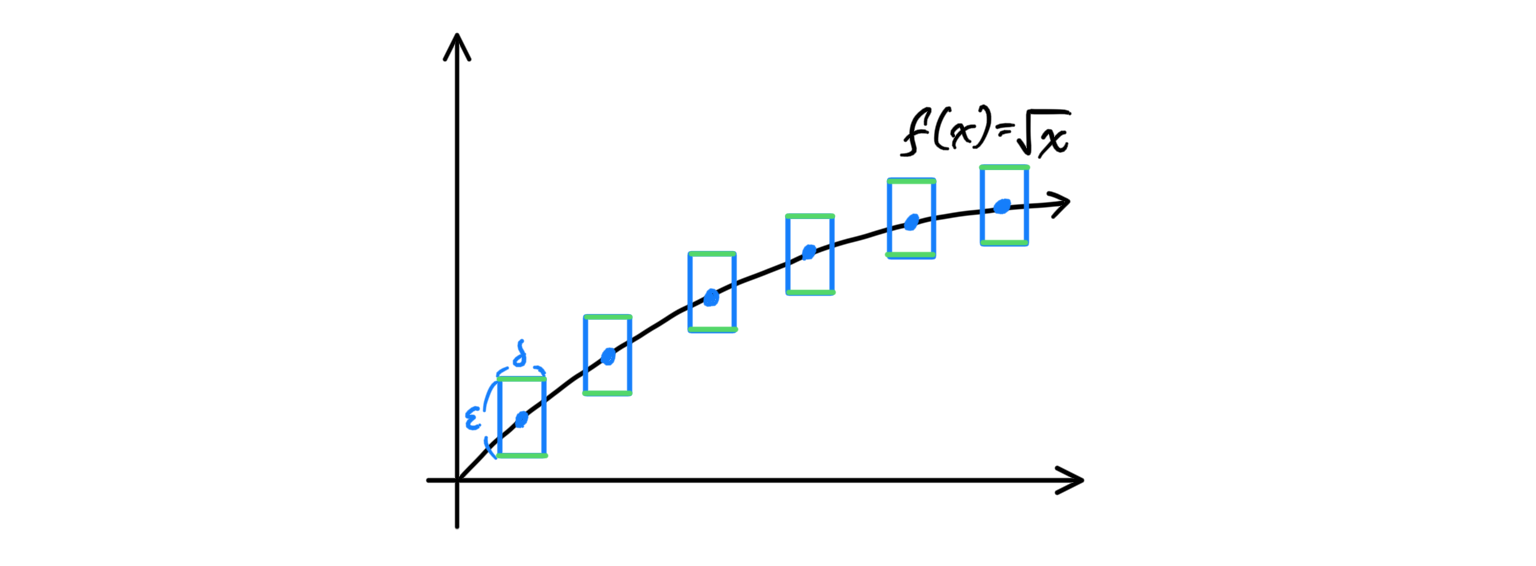
\includegraphics[scale=0.28]{img/Uniform_Continuity_Radical.PNG}
    \end{center}
    We can clearly see that the function $f(x) = 1/x$ is not uniformly continuous, since the graph escapes the $\epsilon \times \delta$ window at some point (marked in red). More strictly speaking, given any length $\epsilon$ of the window, we cannot create a thin-enough $\delta$ box that will contain the graph, since as $x \rightarrow 1$, the function becomes unbounded. 
    \begin{center}
        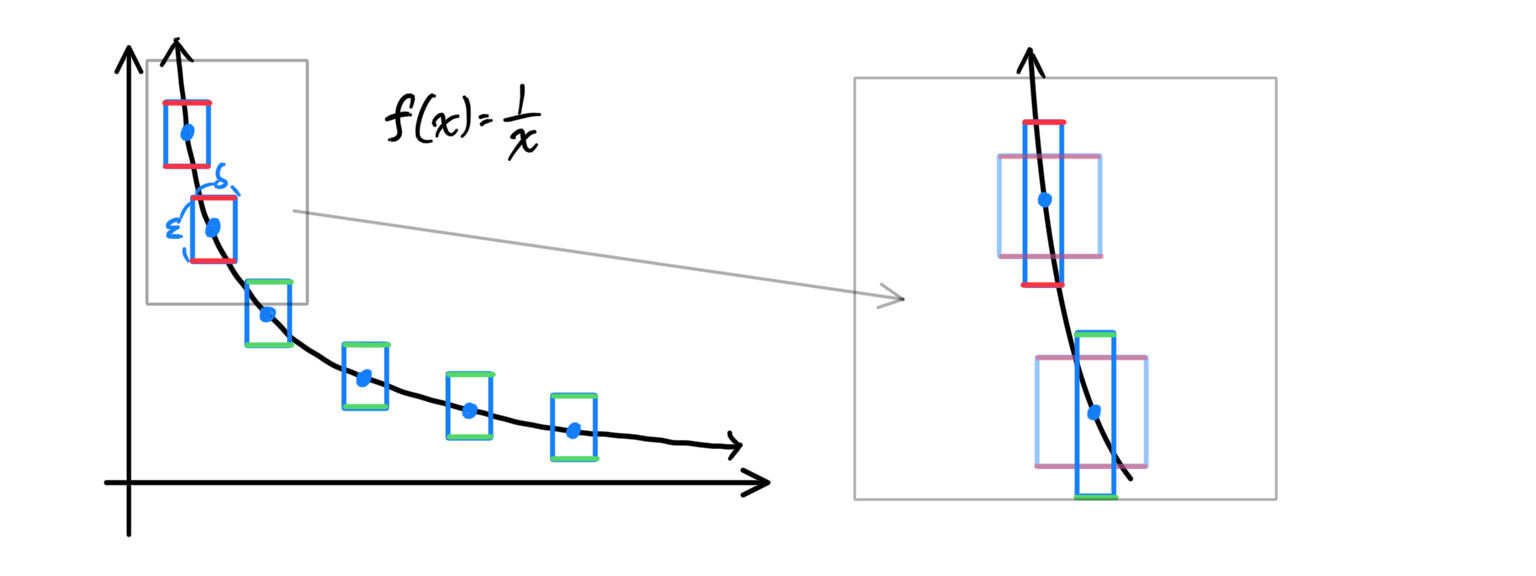
\includegraphics[scale=0.25]{img/Uniform_Continuity_Rational.PNG}
    \end{center}
    That is, arbitrarily thin boxes don't help when the slope is arbitrarily steep. 
  \end{definition}

  To compare uniform continuity with regular continuity, we can adapt this alternate (yet equivalent interpretation): Let there exist function $f: E \longrightarrow \mathbb{R}$. Given any $\epsilon>0$, we can choose a $\delta>0$ such that given any point $x \in E$ and $f(x)$, as long as a second point $y$ is $\delta$ away from $x$, then $f(y)$ is $\epsilon$ away from $f(x)$. This visualization would lead to there being a $2\epsilon \times 2\delta$ window around point $x$. 
  \begin{center}
      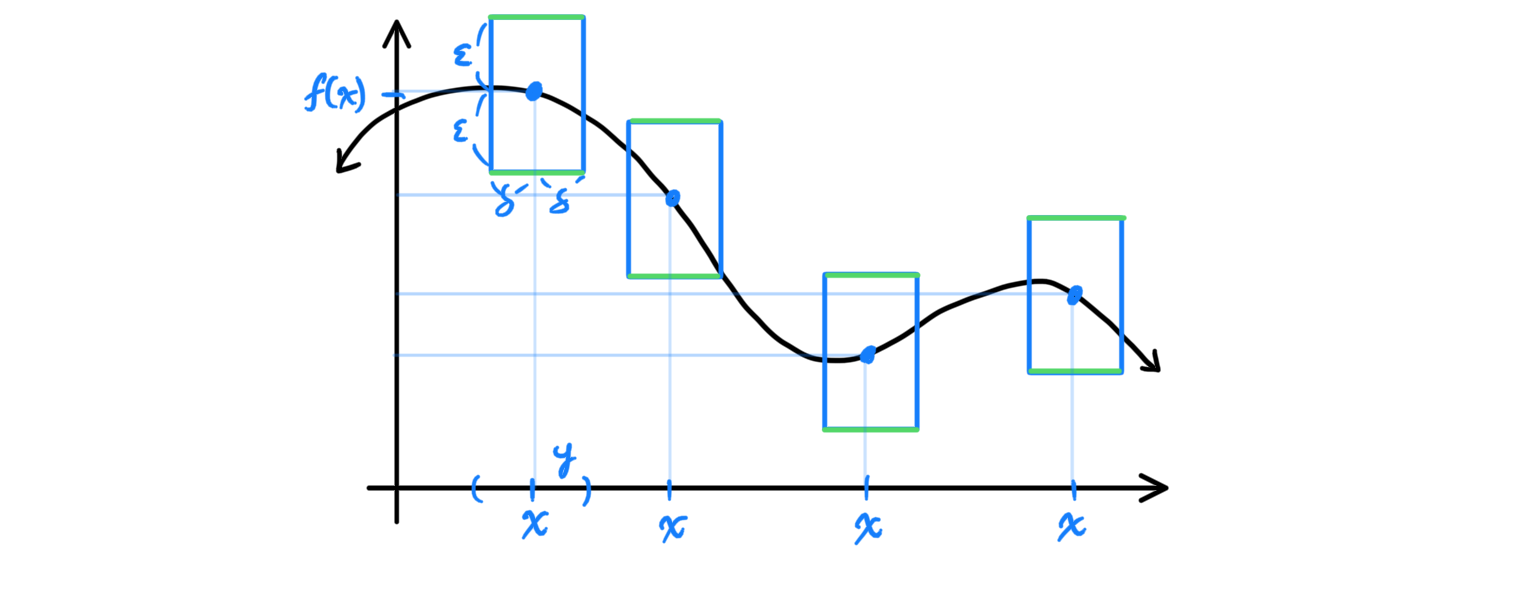
\includegraphics[scale=0.3]{img/Double_Epsilon_Delta_Uniform_Continuity.PNG}
  \end{center}
  Uniform continuity means that the box above does not change dimensions no matter where the point is (hence, the name uniform). Therefore, given a certain $\epsilon > 0$, the way we choose $\delta$ is only dependent on $\epsilon$, and so it must be a function of $\epsilon$: 
  \[\delta = \delta(\epsilon)\]
  However, in continuity, there just has to exist \textbf{some} $\delta$-neighborhood of $x$ such that its image is contained in the $\epsilon$-neighborhood of $f(x)$. There are no restrictions on the dimensions of this box; it just has to exist. 
  \begin{center}
      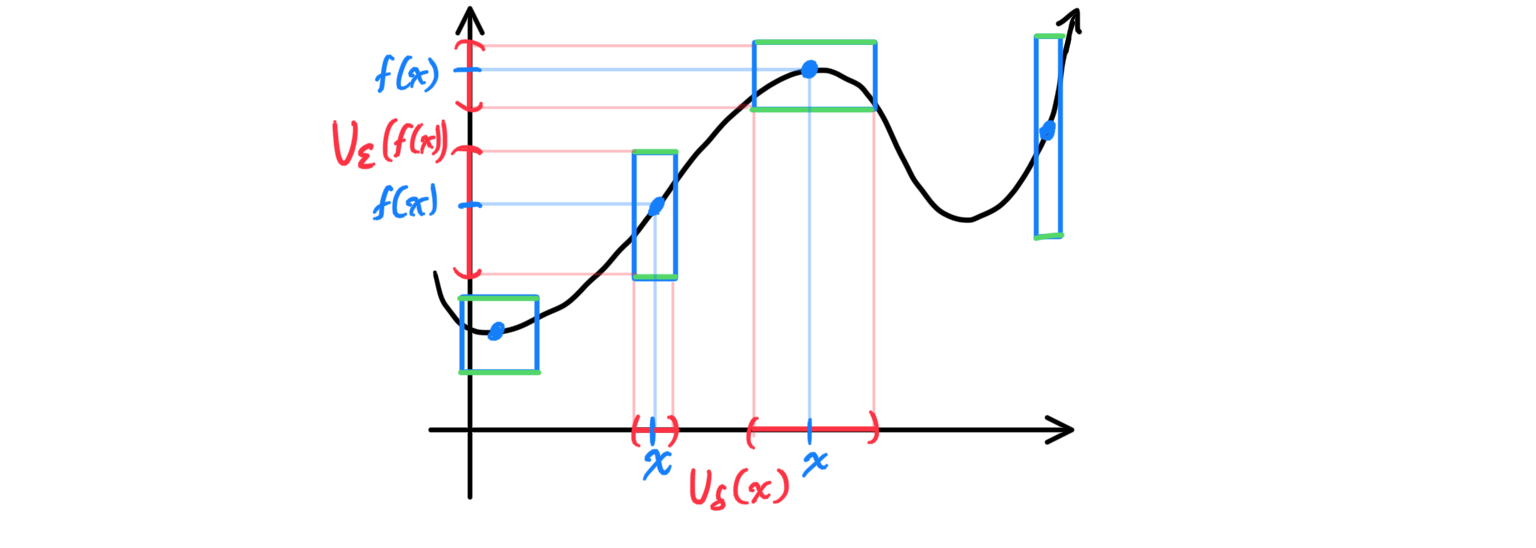
\includegraphics[scale=0.28]{img/Regular_Continuity_Box_Visual.PNG}
  \end{center}

  \begin{lemma}
    If $f$ is uniformly continuous on the set $E$, it is continuous at each point of that set. However, the converse is not generally true. 
  \end{lemma}

  \begin{theorem}[Cantor's Theorem on Uniform Continuity]
  A function that is continuous on a closed interval is uniformly continuous on that interval. 
  \end{theorem}


  \begin{example}
    Let $f: \mathbb{R} \longrightarrow \mathbb{R}, \; f(x) = 3x+7$. Then $f$ is uniformly continuous. Choose $\epsilon > 0$. Let $\delta = \epsilon / 3$. Choose $x, y \in \mathbb{R}$ and assume $|x-y| < \delta$. Then, 
    \[ | f(x) - f(y) | = | 3x + 7 - 3 y - 7 | = 3 |x-y| < 3 \delta = \epsilon\]
  \end{example}

  \begin{example}
    Let $f: (0, 4) \subset \mathbb{R} \longrightarrow \mathbb{R}, \; f(x) = x^2$. Then $f$ is uniformly continuous on $(0, 4)$. Choose $\epsilon > 0$. Let $\delta = \epsilon / 8$. Choose $x, y \in (0, 4)$ and assume $|x-y| < \delta$. Then, 
    \[ |f(x) - f(y)| = |x^2 - y^2| = (x+y) |x-y| < (4+4) |x-y| = 8\delta = \epsilon\]
  \end{example}

  In both examples, the function satisfied an inequality of form 
  \[ |f(x_1) - f(x_2)| \leq M |x_1 - x_2|\]
  this is called the Lipshitz inequality. 

\subsection{Lipshitz Continuity}

  Lipshitz continuity is a strong form of uniform continuity for functions. Intuitively, a Lipshitz continuous function is limited in how fast it can change (by the Lipshitz constant). 

  \begin{definition}[Lipshitz Continuous Function]
    Given $f: E \subset \mathbb{R} \longrightarrow \mathbb{R}$, $f$ is \textbf{Lipshitz continuous} if there exists a positive real constant $M$ such that for all real $x, y \in E$, 
    \[\big| f(x) - f(y) \big| \leq M \big| x - y \big|\]
    The corresponding $M$ is called the \textbf{Lipshitz constant}, and the smallest constant $M$ satisfying this inequality is called the \textbf{best Lipshitz constant}. 

    Note that Lipshitz continuity pops up as a very natural extension of uniform continuity. The inequality above just means that given an $\epsilon$, we can choose a $\delta$ such that a linear multiple of $\delta$ is always greater than $\epsilon$. This means that Lipshitz continuity is just uniform continuity such that the $\delta$ function is linear:  
    \[\delta = \delta(\epsilon) = \frac{1}{M} \epsilon\]
    \begin{center}
        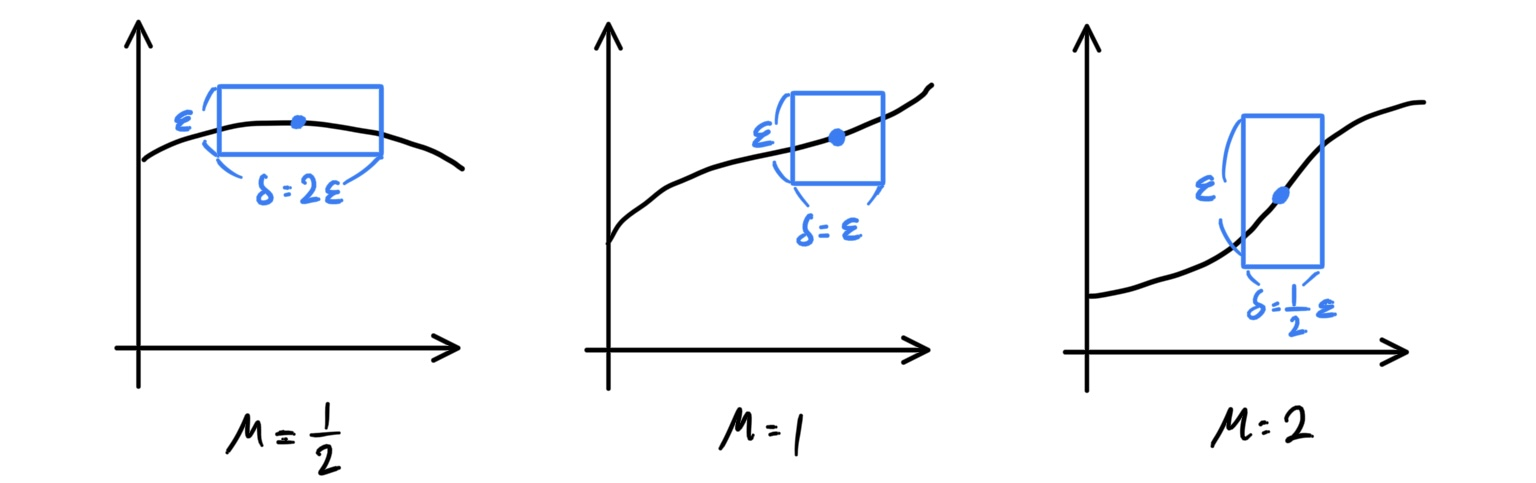
\includegraphics[scale=0.25]{img/Lipshitz_Continuity.jpg}
    \end{center}
  \end{definition}

  Another way to interpret uniform continuity is by seeing that the derivative of $f$ is bounded by the slope $M$. 
  \begin{center}
      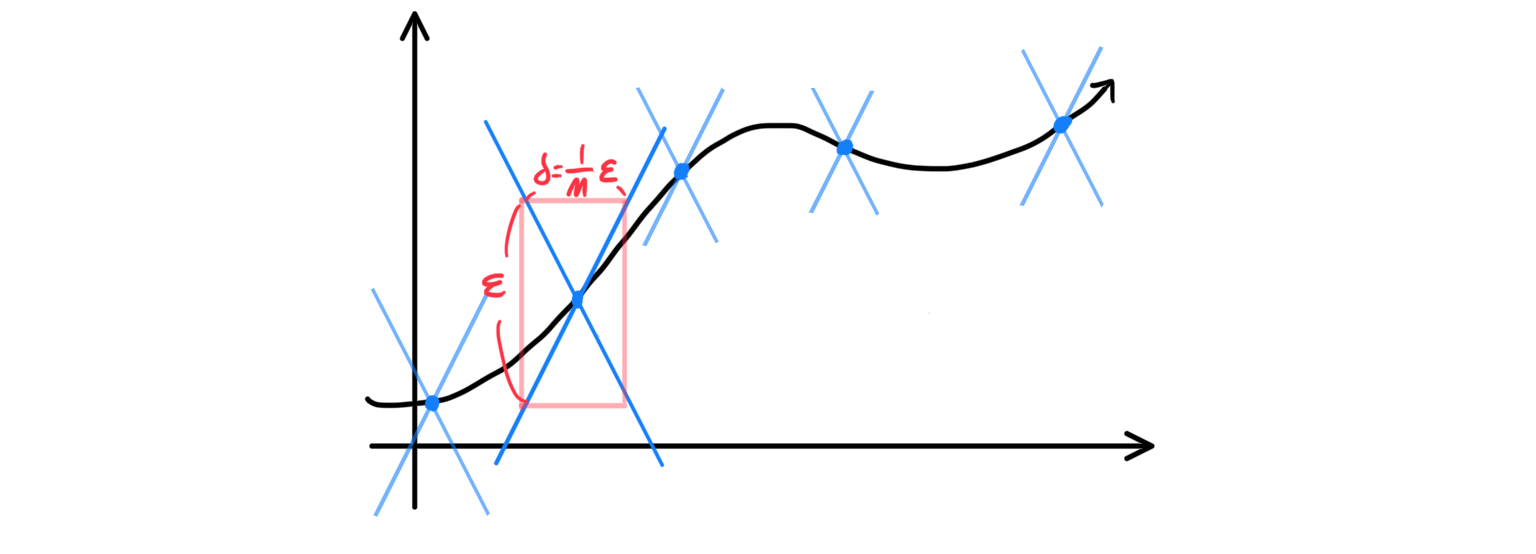
\includegraphics[scale=0.3]{img/Lipshitz_Continuity_Slope_Bound.PNG}
  \end{center}
  This slope bound implies that for every pair of points on the graph of this function, the absolute value of the slope of the line connecting them is not greater than $M'$. The smallest $M'$ is the best Lipshitz constant. 

  \begin{definition}[Bi-Lipshitz Continuity]
    A function $f: E \subset \mathbb{R}$ is \textbf{Bi-Lipshitz continuous} if there exists constant $M\geq 1$ such that for all real $x, y \in E$, 
    \[ \frac{1}{M} |x - y| \leq |f(x) - f(y)| \leq M |x - y|\]
    A visual of this map is shown, where the function $f$ must always land in the shaded green area. 
    \begin{center}
        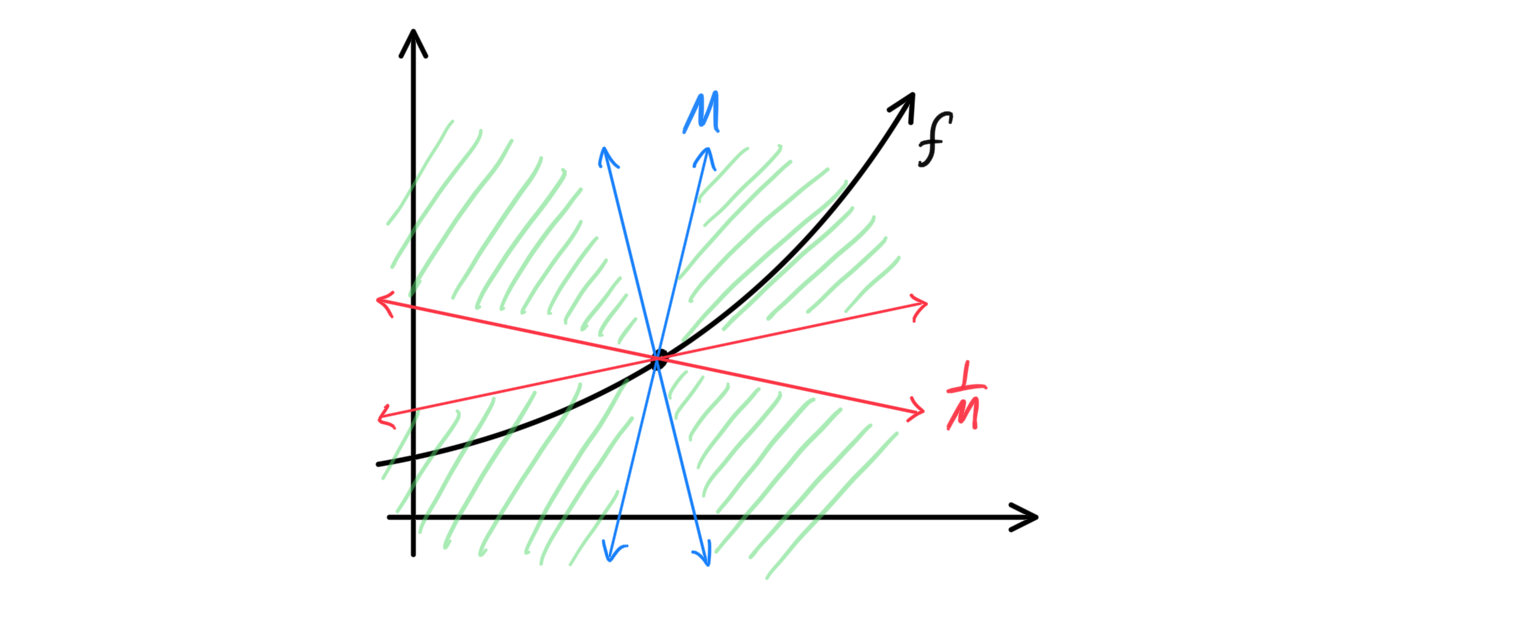
\includegraphics[scale=0.25]{img/BiLipshitz_Map.PNG}
    \end{center}
    It immediately follows that for $x \neq y$, $ |f(x) - f(y)|$ cannot equal $0$, which means that a bilipshitz map is injective. A bilipshitz map is really just Lipshitz map with its inverse also being Lipshitz. 
  \end{definition}

  \begin{proposition}
  A bilipshitz map $f$ is a homeomorphism onto its image. 
  \end{proposition}

\subsection{Discontinuity}

  \begin{definition}[Discontinuity]
    If the function $f: E \longrightarrow \mathbb{R}$ is not continuous at a point of $E$, then this point is called a \textbf{point of discontinuity}, or simply a \textbf{discontinuity} of $f$. 

    That is, $a$ is a point of discontinuity of $f$ if for some neighborhood $V(f(a))$ of $f(a)$, there exists no neighborhood of $a$ whose image under the mapping $f$ is contained in $V(f(a))$. 
    There are three types of discontinuities: 
    \begin{enumerate}
      \item A \textbf{removable discontinuity} is characterized by the fact that the limit $\lim_{x \rightarrow a} f(x) = A$ exists, but $A \neq f(a)$. \begin{center}
          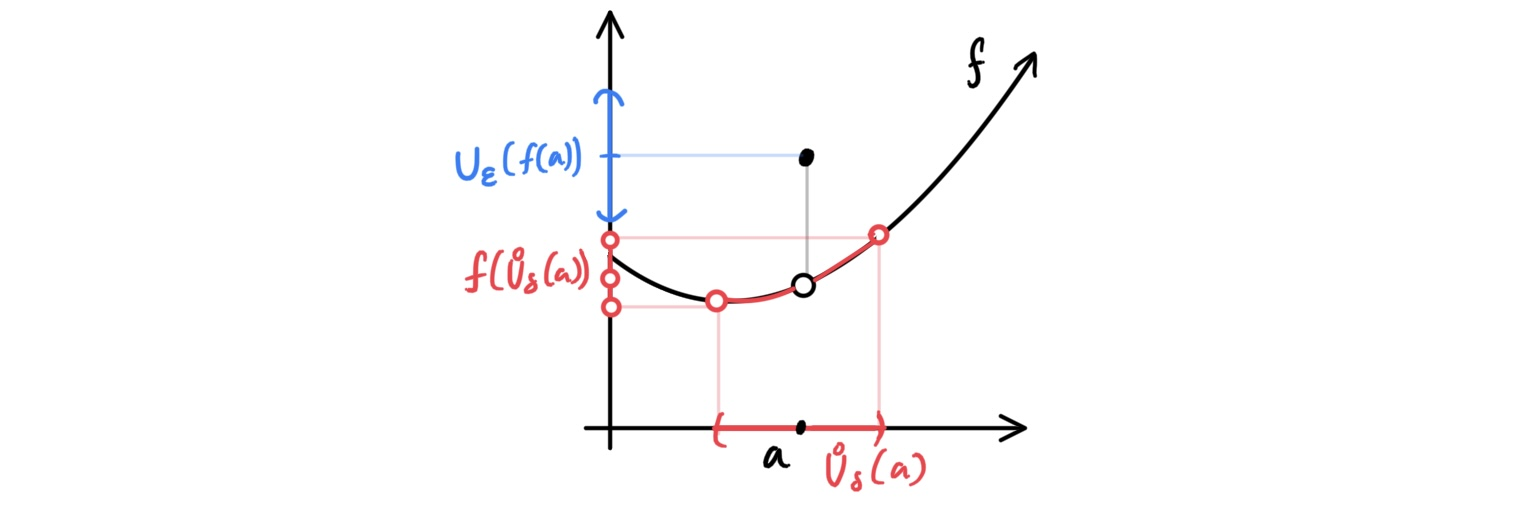
\includegraphics[scale=0.23]{img/Removable_Discontinuity.PNG}
      \end{center}
      This means that we can modify $f$ and define a new function $\Tilde{f}: E \longrightarrow \mathbb{R}$ as
      \[\Tilde{f}(x) = \begin{cases}
      f(x), & x \in E \setminus a \\
      A, & x = a
      \end{cases}\]
      which would be continuous on $E$. 
      \item A \textbf{discontinuity of first kind}, also known as a jump/step discontinuity, is characterized by both the left and right-hand limits 
      \[\lim_{x \rightarrow a-0} f(x) \text{ and } \lim_{x \rightarrow a+0} f(x)\]
      existing, but at least one of them is not equal to the value $f(a)$ that the function assumes at $a$. 
      \begin{center}
          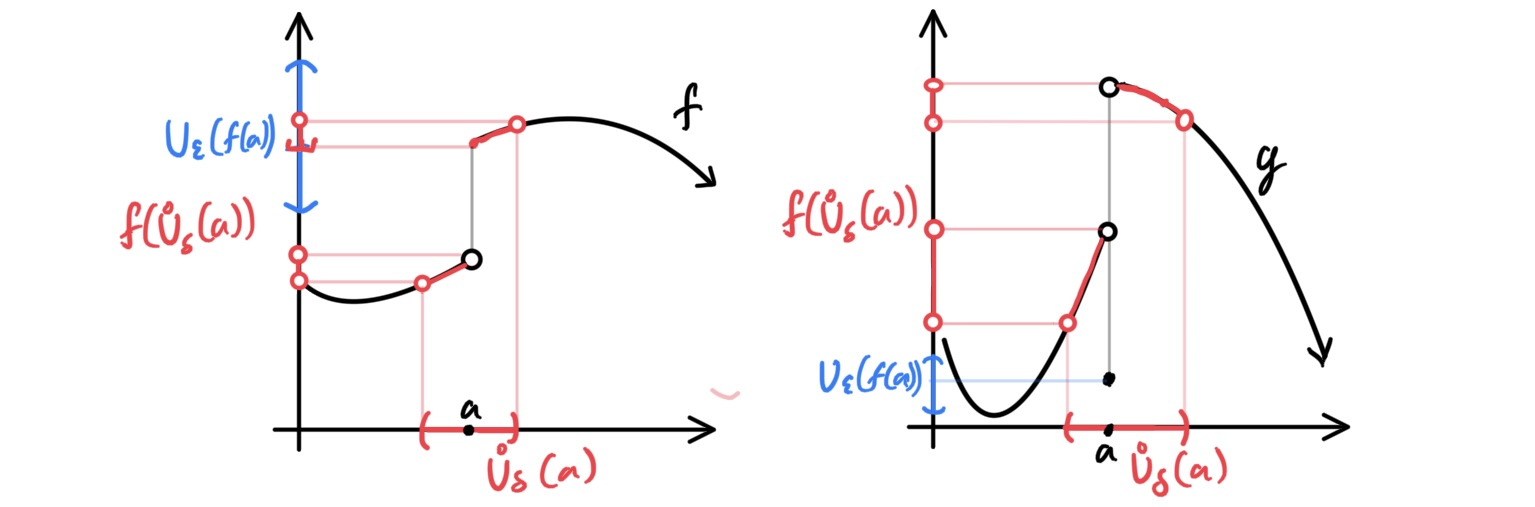
\includegraphics[scale=0.23]{img/Discontinuity_First.PNG}
      \end{center}
      \item A \textbf{discontinuity of second kind}, also known as an essential discontinuity, is characterized by at least one of the two limits 
      \[\lim_{x \rightarrow a-0} f(x) \text{ and } \lim_{x \rightarrow a+0} f(x)\]
      not existing. 
      \begin{center}
          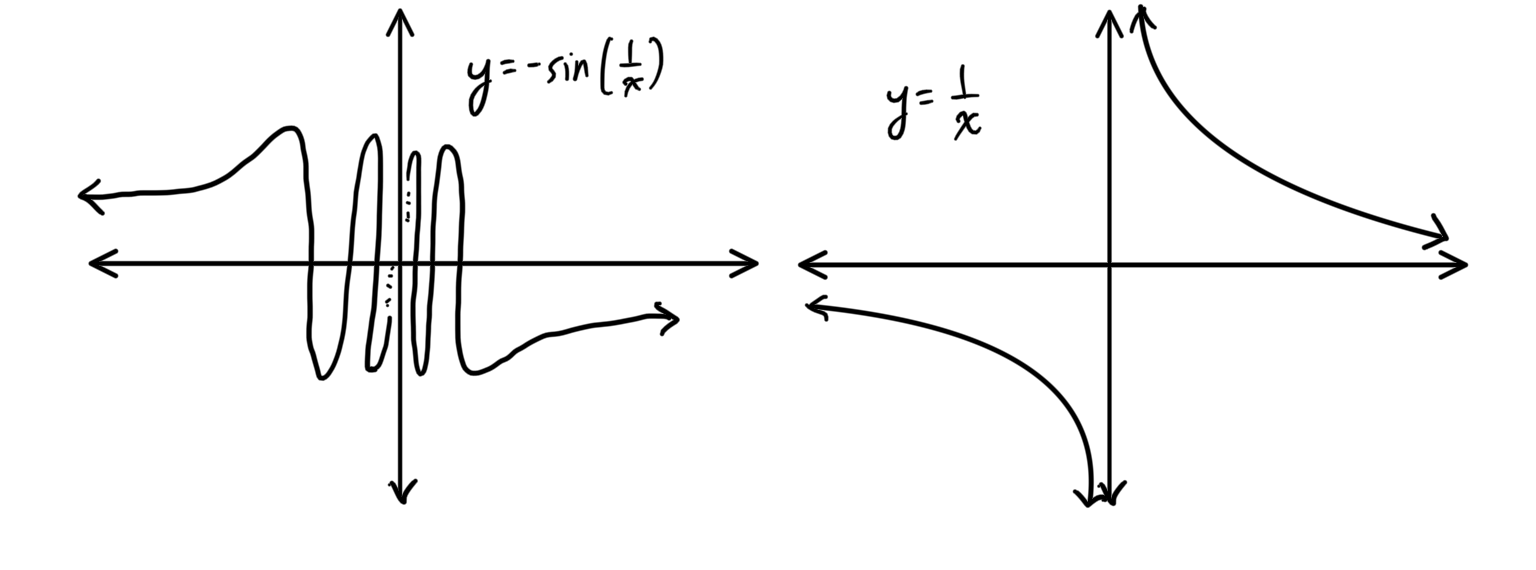
\includegraphics[scale=0.23]{img/Discontinuity_Second.PNG}
      \end{center}
    \end{enumerate}
    Note that strictly speaking, a removable discontinuity is really a discontinuity of first kind, but in this context we distinguish them. 
  \end{definition}

  \begin{example}[Dirichlet Function]
    The Dirichlet function, defined
    \[\mathcal{D}(x) = \begin{cases}
    1, & \text{ if } x \in \mathbb{Q} \\
    0, & \text{ if } x \in \mathbb{R} \setminus \mathbb{Q} 
    \end{cases}\]
    is discontinuous at every point, and obviously all of its discontinuities are of second kind, since in every interval there are both rational and irrational numbers and therefore there exists no limit at any point $a \in \mathbb{R}$. 

    More specifically, given any point $a \in \mathbb{R}$, assume that $a$ is rational. We can set $\epsilon = 0.1$-neighborhood around the value $1$, but no matter how small we let $\delta$, the interval $(a - \delta, a + \delta)$ will contain both rationals and irrationals, meaning that it will map to $\{0,1\}$ always, which is not fully contained in $(0.9, 1.1)$.  
  \end{example}

  Here is a slightly more interesting example. 

  \begin{example}[Riemann Function]
    Let the Riemann function $\mathcal{R}$ be defined
    \[\mathcal{R}(x) = \begin{cases}
    \frac{1}{n}, & \text{ if } x = \frac{m}{n} \in \mathbb{Q}, \text{ where gcd}(m, n) = 1 \\
    0, & \text{ if } x \in \mathbb{R} \setminus \mathbb{Q}
    \end{cases}\]
    We first note that for any point $a \in \mathbb{R}$, any bounded neighborhood $U(a)$ of it, and any number $N \in \mathbb{N}$, the neighborhood $U(a)$ contains only a finite number of rational numbers $\mathbb{m}{n}$, where $n < N$. By shrinking the neighborhood, we can assume that the denominators of all rational numbers in the neighborhood are larger than $N$. We can visualize why this is by seeing that rational numbers with larger denominators have smaller "gaps" between them. 
    \begin{center}
        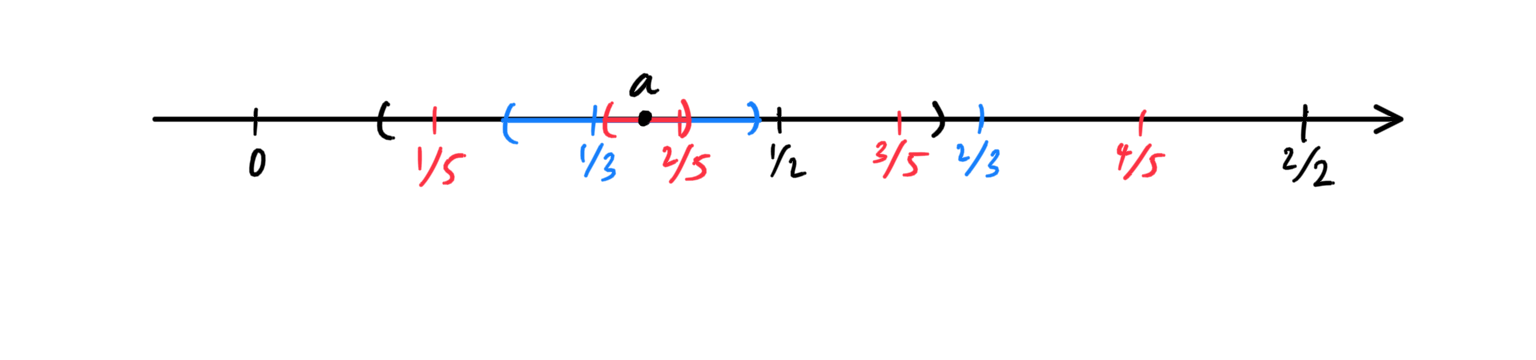
\includegraphics[scale=0.23]{img/Rationals_Spread_Apart.PNG}
    \end{center}
    Thus, at any point $x \in U(a) \setminus a$, we have 
    \[\big| \mathcal{R}(x) \big| < \frac{1}{N}\]
    and therefore
    \[\lim_{x \rightarrow a} \mathcal{R} (x) = 0\]
    at any point $a \in \mathbb{R} \setminus \mathbb{Q}$. Hence, the Riemann function is continuous at any irrational number. 
  \end{example}


 
\section{Differentiation}
 
\section{Riemann and Darboux Integration} 

  We have done integration over closed intervals $[a, b]$. The natural extension is to define integration over \textit{boxes} $B = \prod_i [a_i, b_i]$. Essentially the construction is exactly the same. 

  \begin{definition}[Partition/Mesh]
    Let $B = \prod_i [a_i, b_i] \subset \mathbb{R}^n$ be a box. Then, a \textbf{partition}---or \textbf{mesh}---of $B$ is a finite set of points $P = \{x_{ij}\}_{1 \leq i \leq n, 0 \leq j \leq m_i}$\footnote{Therefore, for each dimension $i$, we want to take the interval $[a_i, b_i]$ and subdivide it into $m_i+1$ subintervals.} s.t. 
    \begin{equation}
      a_i = x_{i, 0} \leq x_{i, 1} \leq x_{i, 2} \leq \ldots \leq x_{i, m_i-1} \leq x_{i, m_i} = b \quad \forall i = 1, \ldots, n
    \end{equation}
    We denote each \textbf{box} within the partition as 
    \begin{equation}
      \Delta_J = \Delta_{j_1, j_2, \ldots, j_n} = \prod_{i} [x_{i, j_k-1}, x_{i, j_k}] \quad \forall j_i = 1, \ldots, m_i
    \end{equation}
    of volume $|\Delta_J| \coloneqq \prod_{i} (x_{i, j_k} - x_{i, j_{k-1}})$. 
  \end{definition}

  This nearly\footnote{since boundaries overlap} partitions $B$ into a grid of $\prod_i m_i$ smaller boxes, and can be seen as a discretization of the integral which we will construcct. 

  \begin{definition}[Riemann Sums with Respect to Partition]
    Let $P$ be a partition of $B \in \mathbb{R}^n$ and let $f: B \subset \mathbb{R}^n \to \mathbb{R}$ be bounded. Then, the \textbf{upper and lower Riemann sums} of $f$ with respect to $P$ are defined 
    \begin{equation}
      U(P, f) \coloneqq \sum_{J} \sup_{x \in \Delta_J} f(x) |\Delta_J|, \qquad L(P, f) \coloneqq \sum_{J} \inf_{x \in \Delta_J} f(x) |\Delta_J|
    \end{equation}

    \begin{figure}[H]
      \centering
      \begin{subfigure}[b]{0.48\textwidth}
        \centering
        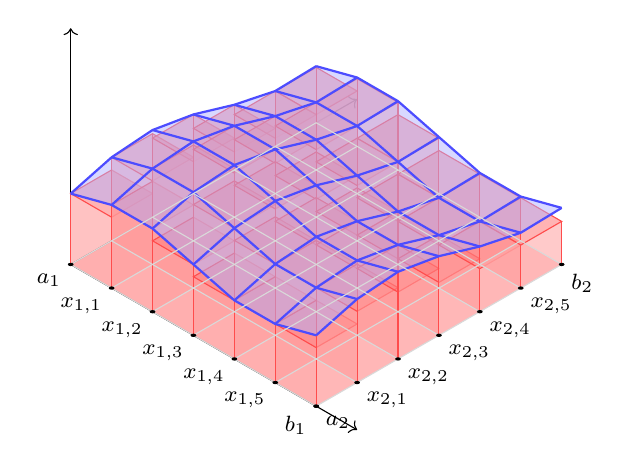
\begin{tikzpicture}[scale=0.6,
          x={(0.866cm,-0.5cm)}, y={(0.866cm,0.5cm)}, z={(0cm,1cm)}]
          
          % Draw axes (without labels)
          \draw[->] (0,0,0) -- (7,0,0);
          \draw[->] (0,0,0) -- (0,7,0);
          \draw[->] (0,0,0) -- (0,0,5);
          
          % Draw rectangular prisms (lower Riemann sum)
          % Using minimum z-value in each cell for lower sum
          \foreach \x in {0,1,2,3,4,5} {
            \foreach \y in {0,1,2,3,4,5} {
              % Calculate heights at four corners of the cell
              \pgfmathsetmacro{\zaa}{1.5 + 0.3*sin(\x*60) + 0.35*sin(\y*50)}
              \pgfmathsetmacro{\zba}{1.5 + 0.3*sin((\x+1)*60) + 0.35*sin(\y*50)}
              \pgfmathsetmacro{\zbb}{1.5 + 0.3*sin((\x+1)*60) + 0.35*sin((\y+1)*50)}
              \pgfmathsetmacro{\zab}{1.5 + 0.3*sin(\x*60) + 0.35*sin((\y+1)*50)}
              
              % Find minimum height (lower Riemann sum)
              \pgfmathsetmacro{\zmin}{min(\zaa,min(\zba,min(\zbb,\zab)))}
              
              % Bottom face (on xy-plane)
              \fill[red!30, opacity=0.6] (\x,\y,0) -- (\x+1,\y,0) -- (\x+1,\y+1,0) -- (\x,\y+1,0) -- cycle;
              
              % Front face
              \fill[red!40, opacity=0.6] (\x,\y,0) -- (\x+1,\y,0) -- (\x+1,\y,\zmin) -- (\x,\y,\zmin) -- cycle;
              
              % Right face
              \fill[red!35, opacity=0.6] (\x+1,\y,0) -- (\x+1,\y+1,0) -- (\x+1,\y+1,\zmin) -- (\x+1,\y,\zmin) -- cycle;
              
              % Top face
              \fill[red!50, opacity=0.6] (\x,\y,\zmin) -- (\x+1,\y,\zmin) -- (\x+1,\y+1,\zmin) -- (\x,\y+1,\zmin) -- cycle;
              
              % Draw edges
              \draw[red!70] (\x,\y,0) -- (\x,\y,\zmin);
              \draw[red!70] (\x+1,\y,0) -- (\x+1,\y,\zmin);
              \draw[red!70] (\x+1,\y+1,0) -- (\x+1,\y+1,\zmin);
              \draw[red!70] (\x,\y+1,0) -- (\x,\y+1,\zmin);
              \draw[red!70] (\x,\y,\zmin) -- (\x+1,\y,\zmin) -- (\x+1,\y+1,\zmin) -- (\x,\y+1,\zmin) -- cycle;
            }
          }
          
          % Draw surface patches first (back to front for proper layering)
          \foreach \ystart/\yend in {0/1, 1/2, 2/3, 3/4, 4/5, 5/6} {
            \foreach \xstart/\xend in {0/1, 1/2, 2/3, 3/4, 4/5, 5/6} {
              \pgfmathsetmacro{\zaa}{1.5 + 0.3*sin(\xstart*60) + 0.35*sin(\ystart*50)}
              \pgfmathsetmacro{\zba}{1.5 + 0.3*sin(\xend*60) + 0.35*sin(\ystart*50)}
              \pgfmathsetmacro{\zbb}{1.5 + 0.3*sin(\xend*60) + 0.35*sin(\yend*50)}
              \pgfmathsetmacro{\zab}{1.5 + 0.3*sin(\xstart*60) + 0.35*sin(\yend*50)}
              
              \fill[blue!30, opacity=0.5] 
                (\xstart,\ystart,\zaa) --
                (\xend,\ystart,\zba) --
                (\xend,\yend,\zbb) --
                (\xstart,\yend,\zab) -- cycle;
            }
          }
          
          % Draw grid lines on surface
          % Lines parallel to x-axis
          \foreach \y in {0,1,2,3,4,5,6} {
            \draw[blue!70, thick] 
              (0,\y,{1.5 + 0.35*sin(\y*50)}) 
              \foreach \x in {1,2,3,4,5,6} {
                -- (\x,\y,{1.5 + 0.3*sin(\x*60) + 0.35*sin(\y*50)})
              };
          }
          
          % Lines parallel to y-axis
          \foreach \x in {0,1,2,3,4,5,6} {
            \draw[blue!70, thick] 
              (\x,0,{1.5 + 0.3*sin(\x*60)}) 
              \foreach \y in {1,2,3,4,5,6} {
                -- (\x,\y,{1.5 + 0.3*sin(\x*60) + 0.35*sin(\y*50)})
              };
          }
          
          % Base grid
          \foreach \x in {0,1,2,3,4,5,6} {
            \draw[gray!30, thin] (\x,0,0) -- (\x,6,0);
            \draw[gray!30, thin] (0,\x,0) -- (6,\x,0);
          }
          
          % X-axis tick labels (back axis)
          \foreach \x/\label in {0/a_1, 1/x_{1,1}, 2/x_{1,2}, 3/x_{1,3}, 4/x_{1,4}, 5/x_{1,5}, 6/b_1} {
            \fill (\x,0,0) circle (0.05);
            \node[below left, font=\footnotesize] at (\x,0,0) {$\label$};
          }
          
          % Y-axis tick labels (front axis at x=6)
          \foreach \y/\label in {0/a_2, 1/x_{2,1}, 2/x_{2,2}, 3/x_{2,3}, 4/x_{2,4}, 5/x_{2,5}, 6/b_2} {
            \fill (6,\y,0) circle (0.05);
            \node[below right, font=\footnotesize] at (6,\y,0) {$\label$};
          }
        \end{tikzpicture}
        \caption{Lower Riemann sum.}
        \label{fig:lower_riemann_sum}
      \end{subfigure}
      \hfill 
      \begin{subfigure}[b]{0.48\textwidth}
        \centering
        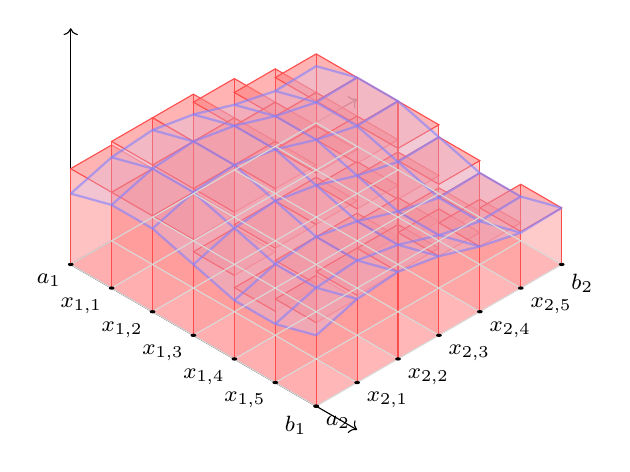
\begin{tikzpicture}[scale=0.6,
          x={(0.866cm,-0.5cm)}, y={(0.866cm,0.5cm)}, z={(0cm,1cm)}]
          
          % Draw axes (without labels)
          \draw[->] (0,0,0) -- (7,0,0);
          \draw[->] (0,0,0) -- (0,7,0);
          \draw[->] (0,0,0) -- (0,0,5);
          
          % Draw rectangular prisms (upper Riemann sum)
          % Using maximum z-value in each cell for upper sum
          \foreach \x in {0,1,2,3,4,5} {
            \foreach \y in {0,1,2,3,4,5} {
              % Calculate heights at four corners of the cell
              \pgfmathsetmacro{\zaa}{1.5 + 0.3*sin(\x*60) + 0.35*sin(\y*50)}
              \pgfmathsetmacro{\zba}{1.5 + 0.3*sin((\x+1)*60) + 0.35*sin(\y*50)}
              \pgfmathsetmacro{\zbb}{1.5 + 0.3*sin((\x+1)*60) + 0.35*sin((\y+1)*50)}
              \pgfmathsetmacro{\zab}{1.5 + 0.3*sin(\x*60) + 0.35*sin((\y+1)*50)}
              
              % Find maximum height (upper Riemann sum)
              \pgfmathsetmacro{\zmax}{max(\zaa,max(\zba,max(\zbb,\zab)))}
              
              % Bottom face (on xy-plane)
              \fill[red!30, opacity=0.6] (\x,\y,0) -- (\x+1,\y,0) -- (\x+1,\y+1,0) -- (\x,\y+1,0) -- cycle;
              
              % Front face
              \fill[red!40, opacity=0.6] (\x,\y,0) -- (\x+1,\y,0) -- (\x+1,\y,\zmax) -- (\x,\y,\zmax) -- cycle;
              
              % Right face
              \fill[red!35, opacity=0.6] (\x+1,\y,0) -- (\x+1,\y+1,0) -- (\x+1,\y+1,\zmax) -- (\x+1,\y,\zmax) -- cycle;
              
              % Top face
              \fill[red!50, opacity=0.6] (\x,\y,\zmax) -- (\x+1,\y,\zmax) -- (\x+1,\y+1,\zmax) -- (\x,\y+1,\zmax) -- cycle;
              
              % Draw edges
              \draw[red!70] (\x,\y,0) -- (\x,\y,\zmax);
              \draw[red!70] (\x+1,\y,0) -- (\x+1,\y,\zmax);
              \draw[red!70] (\x+1,\y+1,0) -- (\x+1,\y+1,\zmax);
              \draw[red!70] (\x,\y+1,0) -- (\x,\y+1,\zmax);
              \draw[red!70] (\x,\y,\zmax) -- (\x+1,\y,\zmax) -- (\x+1,\y+1,\zmax) -- (\x,\y+1,\zmax) -- cycle;
            }
          }
          
          % Draw surface patches with lighter opacity
          \foreach \ystart/\yend in {0/1, 1/2, 2/3, 3/4, 4/5, 5/6} {
            \foreach \xstart/\xend in {0/1, 1/2, 2/3, 3/4, 4/5, 5/6} {
              \pgfmathsetmacro{\zaa}{1.5 + 0.3*sin(\xstart*60) + 0.35*sin(\ystart*50)}
              \pgfmathsetmacro{\zba}{1.5 + 0.3*sin(\xend*60) + 0.35*sin(\ystart*50)}
              \pgfmathsetmacro{\zbb}{1.5 + 0.3*sin(\xend*60) + 0.35*sin(\yend*50)}
              \pgfmathsetmacro{\zab}{1.5 + 0.3*sin(\xstart*60) + 0.35*sin(\yend*50)}
              
              \fill[blue!20, opacity=0.25] 
                (\xstart,\ystart,\zaa) --
                (\xend,\ystart,\zba) --
                (\xend,\yend,\zbb) --
                (\xstart,\yend,\zab) -- cycle;
            }
          }
          
          % Draw grid lines on surface (lighter)
          % Lines parallel to x-axis
          \foreach \y in {0,1,2,3,4,5,6} {
            \draw[blue!50, thick, opacity=0.6] 
              (0,\y,{1.5 + 0.35*sin(\y*50)}) 
              \foreach \x in {1,2,3,4,5,6} {
                -- (\x,\y,{1.5 + 0.3*sin(\x*60) + 0.35*sin(\y*50)})
              };
          }
          
          % Lines parallel to y-axis
          \foreach \x in {0,1,2,3,4,5,6} {
            \draw[blue!50, thick, opacity=0.6] 
              (\x,0,{1.5 + 0.3*sin(\x*60)}) 
              \foreach \y in {1,2,3,4,5,6} {
                -- (\x,\y,{1.5 + 0.3*sin(\x*60) + 0.35*sin(\y*50)})
              };
          }
          
          % Base grid
          \foreach \x in {0,1,2,3,4,5,6} {
            \draw[gray!30, thin] (\x,0,0) -- (\x,6,0);
            \draw[gray!30, thin] (0,\x,0) -- (6,\x,0);
          }
          
          % X-axis tick labels (back axis)
          \foreach \x/\label in {0/a_1, 1/x_{1,1}, 2/x_{1,2}, 3/x_{1,3}, 4/x_{1,4}, 5/x_{1,5}, 6/b_1} {
            \fill (\x,0,0) circle (0.05);
            \node[below left, font=\footnotesize] at (\x,0,0) {$\label$};
          }
          
          % Y-axis tick labels (front axis at x=6)
          \foreach \y/\label in {0/a_2, 1/x_{2,1}, 2/x_{2,2}, 3/x_{2,3}, 4/x_{2,4}, 5/x_{2,5}, 6/b_2} {
            \fill (6,\y,0) circle (0.05);
            \node[below right, font=\footnotesize] at (6,\y,0) {$\label$};
          }
        \end{tikzpicture}
        \caption{Upper Riemann sum.}
        \label{fig:upper_riemann_rum}
      \end{subfigure}
      \caption{}
    \end{figure}
  \end{definition}

  \begin{definition}[Riemann Integral]
    Given that $f: B \subset \mathbb{R}^n \to \mathbb{R}$ is bounded, the \textbf{upper and lower Riemann integrals} of $f$ are defined 
    \begin{equation}
      \overline{\int_B} f(x) \,dx \coloneqq \inf_P U(P, f), \qquad \underline{\int_B} f(x) \,dx \coloneqq \sup_P L(P, f) 
    \end{equation}
    If the upper and lower Riemann integrals are equal, then the \textbf{Riemann integral} of $f$ 
    \begin{equation}
      \int_B f(x) \,dx 
    \end{equation}
    is defined as such. Furthermore, $f$ is said to be \textbf{Riemann integrable} over $B$. 
  \end{definition} 

\subsection{Conditions for Integrability} 

  \begin{theorem}[]
    $f: B \subset \mathbb{R}^n \to \mathbb{R}$ continuous means $f$ is integrable over $B$. 
  \end{theorem}

  However, there are some functions with discontinuities that are in fact integrable. 
  \begin{enumerate}
    \item Given that there is a subset $N$ in $B$ with volume $0$ over which $f$ is not defined, we can integrate over $B \setminus N$. In the one and two dimensional cases, 
    \[\int_{B \setminus N} f(x) dx \text{ and } \iint_{B\setminus N} f(x) dA\]
    are well-defined. Visually, 
    \begin{center}
      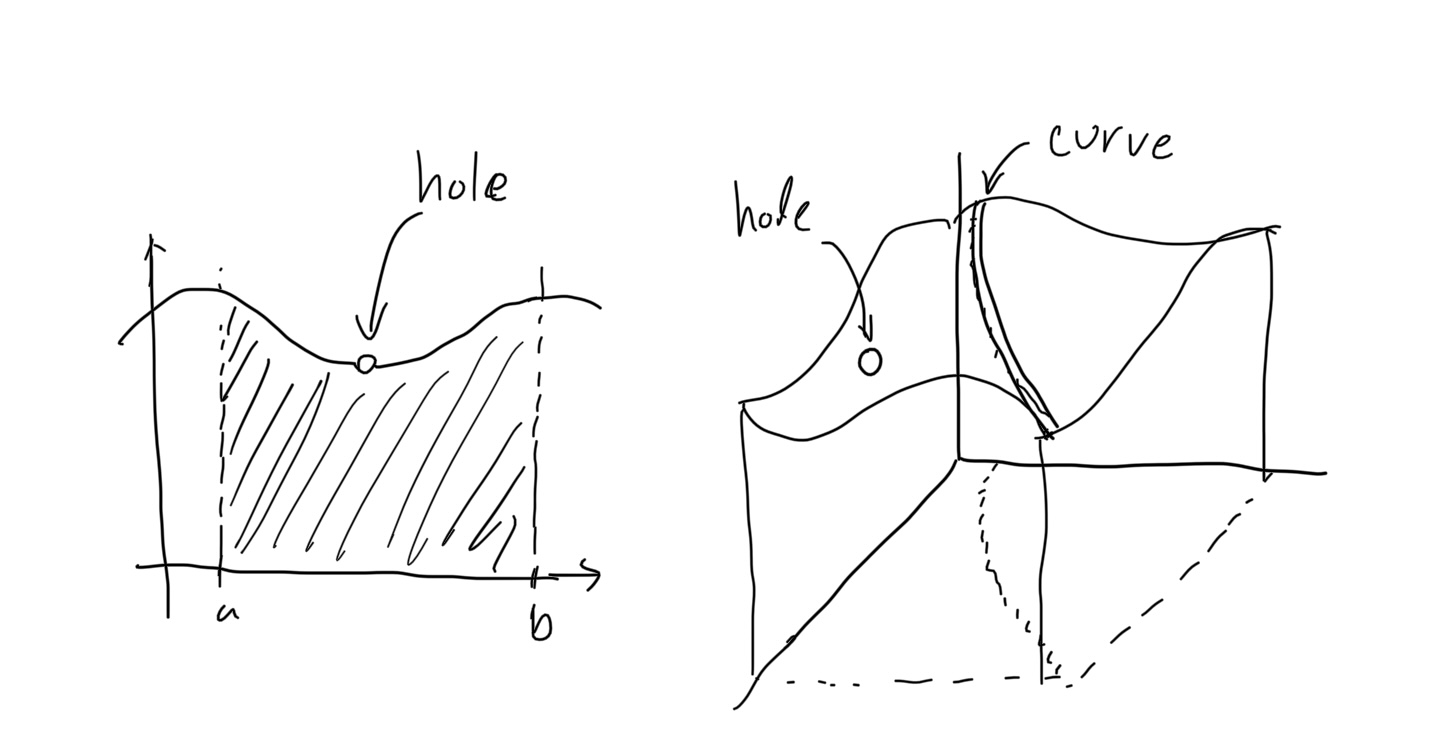
\includegraphics[scale=0.2]{img/Integrable_Hole_Function.jpg}
    \end{center}
    \item The function is defined for all values in the region, but there is a jump in the value of the function. 
    \begin{center}
      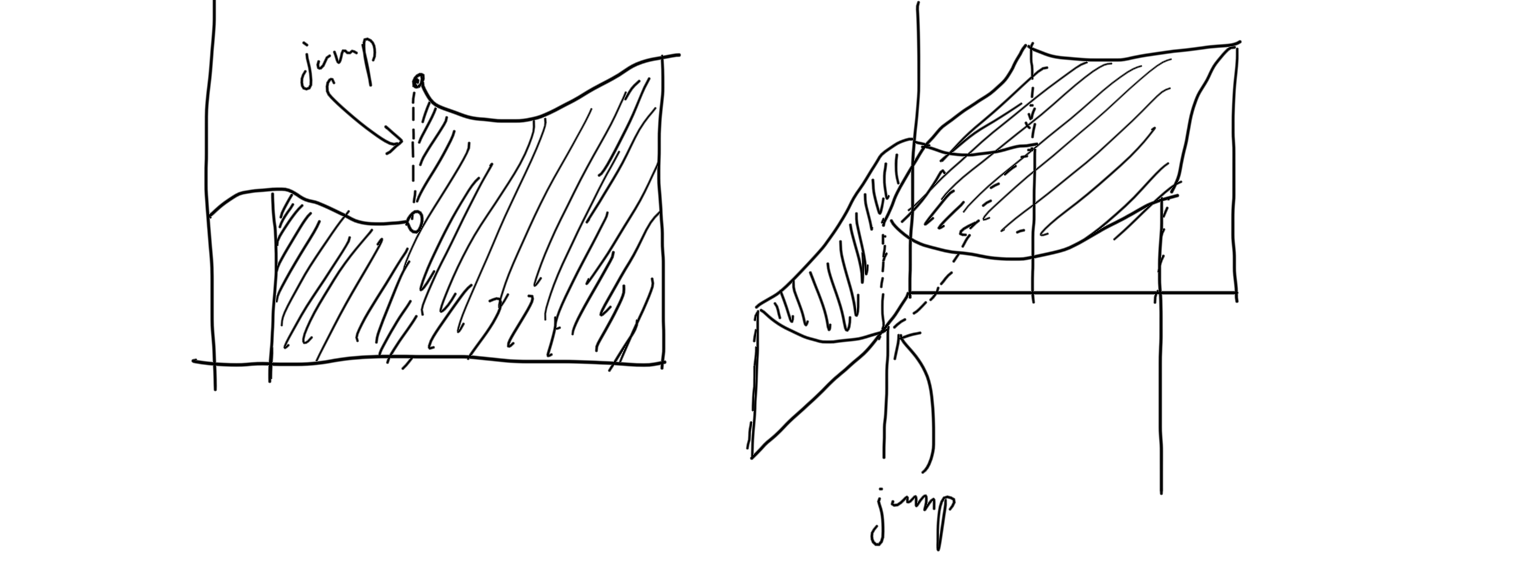
\includegraphics[scale=0.23]{img/Integrable_Jump_Function.PNG}
    \end{center}
  \end{enumerate}
  Informally, if we can visualize the Riemann sum converging to a well-defined area as the rectangles get thinner and thinner, then a discontinuous function is integrable. Indeed, all continuous functions (over a bounded set) are integrable since their Riemann sums are well defined. 


\subsection{Iterated Integrals and Fubini's Theorem} 

  The construction of the integral is one step, but we should know how to practically compute such an integral. We can do this by recursively ``reducing'' the dimension of the region of the integral until we can work with one dimension. This is known as \textit{Cavalieri's principle}: Let $S$ be a bounded $n$-dimensional solid in $\mathbb{R}^n$. Define an $n-1$ subspace $P$ in $\mathbb{R}^n$ and given the quotient space $\mathbb{R}^n / P$ with elements $P_x$, let 
  \begin{equation}
    S \subset \bigcup_{a \leq x \leq b} P_x
  \end{equation}
  That is, $S$ is "in between" affine subspaces $P_a$ and $P_b$. Given the cross section of $S$ with $P_x$, defined $P_x \cap S$, denote the integral of this cross section as $A(x)$. Then, colloquially, the volume of $S$ can be represented as the integral $\int_a^b A(x)\,dx$. This idea basically says that the volume of $S$ is the sum of the areas of its infinitesimal cross sections. 

  \begin{figure}[H]
    \centering 
    
\includegraphics[scale=0.27]{img/Cavalieri_Principle.PNG}
    \caption{Visual of Cavalieri's principle.} 
    \label{fig:cavalieri}
  \end{figure}

  Given a solid $S \subset \mathbb{R}^n$, it is easy to see that no matter what subspace $P$ we choose–that is, no matter what orientation we choose to "cut" the solid– the sum of all of its cross sections should be equal to the true volume of $S$. In the case when $S$ is a box in $\mathbb{R}^n$, Fubini's theorem states that whether we cut $S$ up along the $x_1$-axis, $x_2$-axis, ..., or the $x_n$-axis, the symmetry in volume is always preserved. This theorem is really just a specific case of this general symmetry in volume. 

  \begin{theorem}[Fubini's Theorem]
    Given a function $f: \mathbb{R}^n \longrightarrow \mathbb{R}$, let 
    \[B \equiv \prod_{i=1}^n [\alpha_i, \beta_i]\]
    and let 
    $p$ be any permutation of the elements $\{x_1, x_2, ..., x_n\}$. Then 
    \begin{align*}
        \int_B f \; d V & = \int_{\alpha_n}^{\beta_n} ... \int_{\alpha_1}^{\beta_1} f(x_1,x_2,...,x_n) \; d x_1 ... d x_n \\
        & = \int_{p(\alpha_n)}^{p(\beta_n)} ... \int_{p(\alpha_1)}^{p(\beta_1)} f(x_1,x_2, ..., x_n) \; d p(x_1) ... d p(x_n) 
    \end{align*}
    In the two dimensional case, we have
    \begin{align*}
        \iint_B f \; d A & = \int_c^d \int_a^b f(x, y) \; d x \, d y = \int_a^b \int_c^d f(x, y) \; d y \, d x 
    \end{align*}
    \begin{center}
        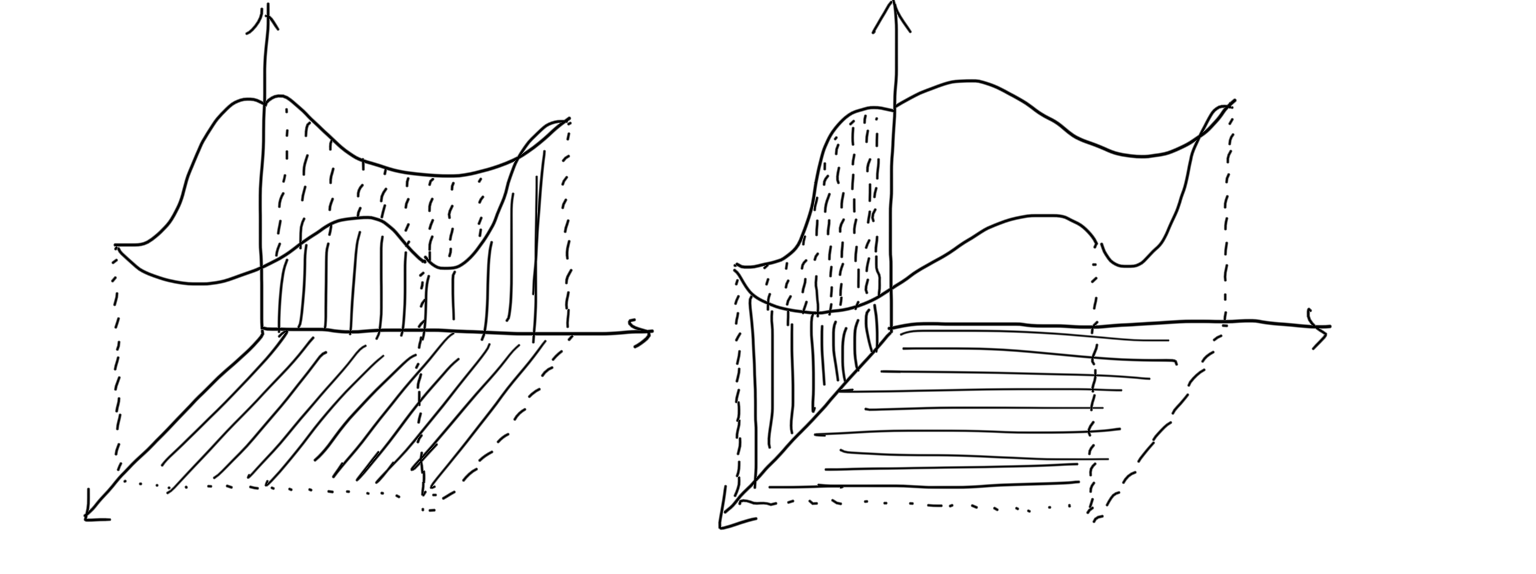
\includegraphics[scale=0.27]{img/Fubini_Theorem.PNG}
    \end{center}
    In the three dimensional case, we have
    \begin{align*}
        \iiint_B f \; d V & 
        = \int_e^f \int_c^d \int_a^b f(x, y, z) \; d x \, d y \, d z = \int_e^f \int_a^b \int_c^d f(x, y, z) \; d y \, d x \, d z \\
        & = \int_c^d \int_a^b \int_e^f f(x, y, z) \; d z \, d x \, d y = \int_c^d \int_e^f \int_a^b f(x, y, z) \; d x \, d z \, d y \\
        & = \int_a^b \int_e^f \int_c^d f(x, y, z) \; d y \, d z \, d x = \int_a^b \int_c^d \int_e^f f(x, y, z) \; d z \, d y \, d x 
    \end{align*}
  \end{theorem}

  Computation of these integrals is simple. You do the innermost integral first with respect to the corresponding variable, while treating the rest of the variables constant. Evaluating each integral outputs a formula for a higher dimensional cross section of the solid $S$. It is clear that computing iterated integrals is really just doing Cavalieri's principle repeatedly. 

\subsection{Integration over Regions between Curves} 

  \begin{definition}[Simple Regions w.r.t. a Variable]
    A bounded region $D$ in $\mathbb{R}^n$ is said to be $x_i$-simple if it is bounded by the graphs of two continuous functions $u_1, u_2: \mathbb{R}^{n-1} \longrightarrow \mathbb{R}$ of the variables 
    \[x_1, x_2, ..., x_{i-1}, x_{i+1}, ..., x_n\]
    That is, $D$ can be expressed in the form 
    \[\{ x \in \mathbb{R}^n \; | \; u_1 (x_1,..., x_{i-1}, x_{i+1}, ... , x_n) \leq x_i \leq u_2 (x_1, ..., x_{i-1}, x_{i+1}, ..., x_n)\}\]
    If a region is simple in all of its variables, it is simply called \textit{simple}. Note that $n$-dimensional boxes are simple regions. 
  \end{definition}

  \begin{example}
    In $\mathbb{R}^2$, the region on the left graph is an $y$-simple region and the region on the right is a $x$-simple region. 
    \begin{center}
    \begin{tikzpicture}[scale=0.8]
      \draw[<->] (-1,0)--(5,0);
      \draw[<->] (0,-1)--(0,5);
      \draw[<->] (6,0)--(12,0);
      \draw[<->] (7,-1)--(7,5);
      \draw plot [smooth] coordinates {(0.6, 1.2) (1,1) (2,1.4) (3,1.3) (4,1.5) (4.3,1.7)};
      \draw plot [smooth] coordinates {(0.6, 3.9) (1,4.1) (2,4) (3,4.3) (4,4.2) (4.3,4.1)};
      \draw[dashed] (0.6,1.2)--(0.6,3.9);
      \draw[dashed] (4.3,1.7)--(4.3,4.1);
      \draw plot [smooth] coordinates {(8.2,0.6) (8,1) (8.4,2) (8.3,3) (8.5,4) (8.7,4.3)};
      \draw plot [smooth] coordinates {(10.9,0.6) (11.1,1) (11,2) (11.3,3) (11.2,4) (11.1,4.3)};
      \draw[dashed] (8.2,0.6)--(10.9,0.6);
      \draw[dashed] (8.7,4.3)--(11.1,4.3);
      \node[below] at (4.8,0) {$x$};
      \node[below] at (11.8,0) {$x$};
      \node[left] at (0,4.8) {$y$};
      \node[left] at (7,4.8) {$y$};
      \node[above] at (3,4.2) {$u_1$};
      \node[above] at (3,1.3) {$u_2$};
      \node[left] at (8.3, 3) {$v_1$};
      \node[right] at (11.3, 3) {$v_2$};
      \draw[fill] (0.6,0) circle (0.05);
      \node[below] at (0.6,0) {$a$};
      \draw[fill] (4.3,0) circle (0.05);
      \node[below left] at (4.3,0) {$b$};
      \draw[fill] (7,0.6) circle (0.05);
      \draw[fill] (7,4.3) circle (0.05);
      \node[left] at (7,0.6) {$c$};
      \node[left] at (7,4.3) {$d$};
    \end{tikzpicture}
    \end{center}
  \end{example}

  We now describe the method of calculating double integrals over elementary regions. 
  \begin{theorem}
  The double integral over a $y$-simple region $D$ bounded by functions $u_1$ and $u_2$ in $\mathbb{R}^2$ and the $x$-values $a$ and $b$ (as shown in the left graph of example 2.1) is
  \[\iint_D f(x, y) = \int_a^b \int_{u_2 (x)}^{u_1 (x)} f(x, y) \, dy \, dx\]
  The double integral over an $x$-simple region $D$ bounded by functions $v_1$ and $v_2$ in $\mathbb{R}^2$ and the $y$-values $c$ and $d$ (shown in the right of graph of example 2.1) is 
  \[\iint_D f(x, y) = \int_c^d \int_{v_2 (y)}^{v_1 (y)} f(x, y) \, dx \, dy\]
  \end{theorem}

  \begin{example}
  Integrating $f(x, y)$ over the unit disk would have the form
  \[\int_{-1}^1 \int_{-\sqrt{1-x^2}}^{\sqrt{1-x^2}} f(x,y) \, dy\, dx \text{ or } \int_{-1}^1 \int_{-\sqrt{1-y^2}}^{\sqrt{1-y^2}} f(x,y) \, dx\, dy \]
  Note that the unit disk is both $x$ and $y$ simple. 
  \end{example}

\subsection{Change of Basis}

  Sometimes, integrating a region over a different basis would make the integral computation much more simpler. In this case, we may be able to transform more complicated regions into elementary regions. We first introduce a change of basis in 2 dimensions and then generalize it into higher dimensions. 
  
  Let $\mathbb{R}^2$ have the standard orthonomal basis $e_1, e_2$, commonly known as the $x, y$ basis. Now, let us construct new basis vectors of $\mathbb{R}^2$, denoted $f_1, f_2$ such that $f_1, f_2$ are functions of $e_1, e_2$. Since they are both bases that span $\mathbb{R}^2$, we can equally represent $e_1, e_2$ as functions of $f_1, f_2$. 
  \begin{align*}
      &e_1 = g(f_1, f_2)\\
      &e_2 = h(f_1, f_2) 
  \end{align*}
  Note that this change of basis does not necessarily have to be linear, as in the context of passive transformation in linear algebra. Then, every point $(x,y)$ in the $(e_1, e_2)$-basis can be rewritten as
  \begin{align*}
      (x, y) & = x e_1 + y e_2 \\
      & = x \, g(f_1, f_2) + y \, h(f_1, f_2) \\
      & = u f_1 + v f_2
  \end{align*}
  Note that it is customary to denote $x, y$ as the coefficients in the $e_1, e_2$ basis and $u, v$ as the coefficients in the new $f_1, f_2$ basis. This way, we can not only write $e_1$ and $e_2$ as functions of $f_1$ and $f_2$, but we can also write the coefficents $x, y$ as functions of the coeffiecents $u, v$! That is, 
  \begin{align*}
      & x = x(u, v) \\
      & y = y(u, v)
  \end{align*}
  which is really just a function 
  \[B: \mathbb{R}^2 \longrightarrow \mathbb{R}^2, \;\; B(u, v) = \begin{pmatrix} x(u, v) \\ y(u, v) \end{pmatrix}\]
  Notice that $B$ changes the $u, v$ coordinates to the $x, y$ coordinates, and $B^{-1}$ changes the $x, y$ coordinates to the $u, v$ coordinates. 
  \[B^{-1}: \mathbb{R}^2 \longrightarrow \mathbb{R}^2, \;\; B^{-1} (x, y) = \begin{pmatrix} u (x, y) \\ v (x, y) \end{pmatrix}\]
  Note that these coefficients actually change \textit{contravariantly}, that is, they change inversely with respect to how the basis vectors are changed. In vector calculus, it is conventional to represent a change of basis with functions that relate the coefficients $x, y$ with $u, v$, rather than the bases $f_1, f_2$ with $e_1, e_2$. 

  \begin{theorem}[Integration over Change of Bases in $\mathbb{R}^2$]
  Let $\mathbb{R}^2$ have the standard orthonomal basis $e_1, e_2$. Now, let us construct new basis vectors of $\mathbb{R}^2$, denoted $f_1, f_2$ such that the coefficients of the vectors in $\mathbb{R}^2$ are related by the change of basis function 
  \[B = \begin{pmatrix} x \\ y \end{pmatrix} \implies B(u, v) = \begin{pmatrix} x(u, v) \\ y(u, v) \end{pmatrix}\]
  Given region $D \subset \mathbb{R}^2$ and $S = B(D)$ is the region transformed by $B$, the integral of function $f(x, y)$ over region $D$ can be expressed as 
  \[\iint_D f(x, y) \, dA = \iint_S f \big( x(u, v), y(u, v) \big) \, \big| J B(u, v) \big| \, d \bar{A}\]
  where $\big| J B(u, v) \big|$ is the determinant of the Jacobian matrix of $B$. Expanding the Facobian determinant gives
  \[\big| J B(u, v) \big| = \frac{\partial x}{\partial u} \frac{\partial y}{\partial v} - \frac{\partial x}{\partial v} \frac{\partial y}{\partial u}\]
  \end{theorem}

  \begin{theorem}[Integration over Change of Bases in $\mathbb{R}^3$]
  Given that we have the change of basis function 
  \[B: \mathbb{R}^3 \longrightarrow \mathbb{R}^3, \;\;\; B(u, v, w) = \begin{pmatrix} x(u, v, w) \\ y(u, v, w) \\ z(u, v, w) \end{pmatrix}\]
  a region $D \in \mathbb{R}^3$ and $S = B(D)$, the region transformed by $B$, the integral of $f(x, y, z)$ over region $D$ can be expressed as 
  \[\iiint_D f(x, y, z)\, dV = \iiint_S f\big( x(u, v, w), y(u, v ,w), z(u, v, w) \big) \big| J B (u, v, w)\big| \, d \bar{V}\]
  where $\big| J B (u, v, w)\big|$ is the Jacobian determinant of $B$. 
  \end{theorem}

  \begin{example}
  Given a real-valued function $f$ defined over the region $D \subset \mathbb{R}^2$, we can perform a change of basis of the $x, y$ coordinates into polar ones within a new region $S$. The change of basis 
  \begin{align*}
      & x = r \cos{\theta} \\
      & y = r \sin{\theta} 
  \end{align*}
  \begin{center}
  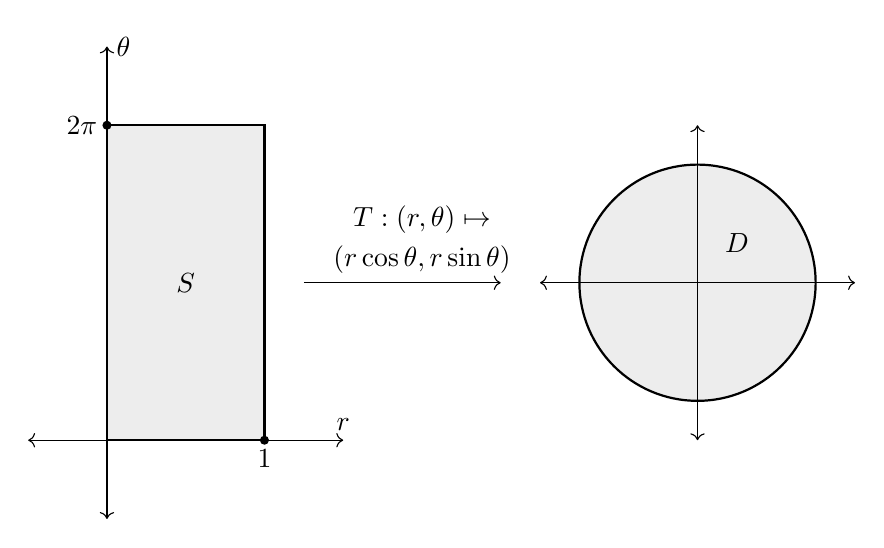
\begin{tikzpicture}
      \draw[thick, fill=lightgray] (7.5,2) circle (1.5);
      \draw[<->] (-1,0)--(3,0);
      \draw[<->] (0,-1)--(0,5);
      \draw[thick, fill=lightgray] (0,0) rectangle (2,4);
      \node at (1,2) {$S$};
      \draw[fill] (0,4) circle (0.05);
      \draw[fill] (2,0) circle (0.05);
      \node[below] at (2,0) {$1$};
      \node[left] at (0,4) {$2 \pi$};
      \node[above] at (3,0) {$r$};
      \node[right] at (0,5) {$\theta$};
      \draw[->] (2.5, 2)--(5,2);
      \node[above] at (4,2.5) {$T: (r, \theta) \mapsto$};
      \node[above] at (4,2) {$ (r \cos{\theta}, r \sin{\theta})$};
      \draw[<->] (5.5,2)--(9.5,2);
      \draw[<->] (7.5,0)--(7.5,4);
      \node at (8,2.5) {$D$};
  \end{tikzpicture}  
  \end{center}
  \end{example}

  \begin{theorem}[Integration over Change of Bases in $\mathbb{R}^n$]
  Let $\mathbb{R}^n$ have the standard orthonormal basis $e_1, e_2, ..., e_n$, and let us construct a new basis $f_1, f_2, ..., f_n$ such that the coefficients of the vectors in $\mathbb{R}^n$ are related with the functions
  \[B: \mathbb{R}^n \longrightarrow \mathbb{R}^n, \;\;\;\; B(u_1, u_2, \ldots, u_n) = \begin{pmatrix}
  x_1 (u_1, \ldots, u_n) \\x_2 (u_1, \ldots, u_n) \\ \vdots \\ x_n (u_1, \ldots, u_n)
  \end{pmatrix}\]
  Given that the region $D \subset \mathbb{R}^n$ is transformed into a new region $S = B(D) \subset \mathbb{R}^n$ under this basis transformation, the integral of function $f(x_1, \ldots, x_n)$ over region $D$ can be expressed as 
  \[\int_D f(x) \, dH = \int_S f \big( x_1(u), x_2(u), ..., x_n (u) \big) \big| J B(u_1, \ldots, u_n)\big| \, d \bar{H}\]
  where the integral on both the left and right hand side represents integration over an $n$-dimensional region, $x$ represents the $n$-tuple $(x_1, \ldots, x_n)$, $u$ represents the $n$-tuple $(u_1, \ldots, u_n)$, and $\big| J B(u_1, \ldots, u_n)\big|$ represents the Jacobian determinant of function $B$. 
  \end{theorem}

  We now describe some common change of basis formulas for polar, cylindrical, and spherical coordinates. 

  \begin{theorem}[Integration in Polar Coordinates]
  \[\iint_{D} f(x, y) \, dx \,dy = \iint_S f(r \cos{\theta}, r \sin{\theta}) r \, dr \, d\theta\]
  \end{theorem}

  \begin{definition}[Cylindrical, Spherical Coordinates]
  In $\mathbb{R}^3$, \textit{cylindrical coordinates} have the following relation to rectangular coordinates. 
  \begin{align*}
      & x = r \cos{\theta} \\
      & y = r \sin{\theta} \\
      & z = z
  \end{align*}
  In $\mathbb{R}^3$, \textit{spherical coordinates} have the following relation to rectangular coordinates. 
  \begin{align*}
      & x = \rho \sin{\phi} \cos{\theta} \\
      & y = \rho \sin{\phi} \sin{\theta} \\
      & z = \rho \cos{\phi}
  \end{align*}
  \end{definition}

  \begin{corollary}[Integration in Cylindrical Coordinates]
  \[\iiint_D f(x, y, z) \, dx \, dy \, dz = \iiint_S f( r \cos{\theta}, r \sin{\theta}, z) r \, dr \, d\theta \, dz\]
  \end{corollary}

  \begin{corollary}[Integration in Spherical Coordinates]
  \[\iiint_D f(x, y, z) \,dx\,dy\,dz = \iiint_S f(\rho \sin{\phi} \cos{\theta}, \rho \sin{\phi} \sin{\theta}, \rho \cos{\phi}) \rho^2 \sin{\theta} \, d\rho \, d\theta \, d\phi\]
  \end{corollary}

  \begin{example}[Gaussian Integral]
  The following is the (un-normalized) probability distribution function of the Gaussian distribution. 
  \[\int_{-\infty}^{\infty} e^{-x^2} \, dx = \sqrt{\pi}\]
  \end{example}

\subsection{Improper Integrals}

  There are generally two types of improper integrals. 
  \begin{enumerate}
    \item The region $D$ integrated over is unbounded. 
    \item The function $f$ that is integrated is unbounded within the region $D$.
  \end{enumerate}

  These types of improper integrals are usually evaluated using a limiting process. When the interval $I$ is unbounded, say $(1, \infty)$, the integral can be evaluated as 
  \[\int_1^\infty \frac{1}{x^2} \,dx = \lim_{b \rightarrow \infty} \int_1^b \frac{1}{x^2} \, dx = \lim_{b\rightarrow \infty} \bigg( 1 - \frac{1}{b} \bigg) = 1\]
  In case 2, we can add a limit at the point where the function $f$ diverges as such. 
  \[\int_0^1 \frac{1}{\sqrt{x}} \, dx = \lim_{a \rightarrow 0} \int_a^1 \frac{1}{\sqrt{x}} \, dx = \lim_{a \rightarrow 0} (2 - 2\sqrt{a}) = 2\]
  We now describe how to integrate over a certain path $p$ embedded in a higher dimensional space $\mathbb{R}^n$, possibly with a scalar or vector field $f$. We must first go over oriented paths. 

  Extending the previous case, we use a multivariate limiting process in $\mathbb{R}^2$. We will first work with case 2, when $f$ is unbounded within the region $D$. Let us define an elementary region $D$ in $\mathbb{R}^2$; without loss of generality, we will make it $y$-simple, meaning that $D$ can be expressed as
    \[D \equiv \{ (x, y) \in \mathbb{R}^2 \; | \; a \leq x \leq b, \; \phi_1 (x) \leq y \leq \phi_2 (x)\}\]
  We can actually assume that the region in which $f$ is unbounded lies in the boundary $\partial D$. This is because if it lied in the interior of $D$, we could split $D$ into pieces across a path that intersects this region with divergent values, evaluate the integrals over the pieces separately, and then sum the integrals. For example, in the rectangular region below, let the dashed line represent the values where the function $f$ diverges. Then, we can split the region into two rectangular regions shown in the right. 
  \begin{center}
  \begin{tikzpicture}
    \draw (0,0) rectangle (3,2);
    \draw[dashed] rectangle (2,0)--(2,2);
    \draw[->] (3.5,1)--(5,1);
    \draw (8,0)--(6,0)--(6,2)--(8,2);
    \draw[dashed] (8,0)--(8,2);
    \draw[dashed] (9,0)--(9,2);
    \draw (9,0)--(10,0)--(10,2)--(9,2);
  \end{tikzpicture}
  \end{center}
  Therefore, assuming that $f$ is unbounded in $\partial D$, we can construct a new region 
  \[D_{\eta, \delta} \equiv \{(x, y) \in \mathbb{R}^2 \; | \; a + \eta \leq x \leq b - \eta, \; \phi_1 (x) + \delta \leq y \leq \phi_2 (x) - \delta\}\]
  for some arbitrarily small numbers $\eta, \delta >0$, meaning that the integral (reduced to iterated integrals using Fubini's theorem) 
  \[F(\eta, \delta) \equiv \iint_{D_{\eta, \delta}} f(x, y) \, dA = \int_{a + \eta}^{b - \eta} \int_{\phi_1 (x) + \delta}^{\phi_2 (x) - \delta} f(x, y) \, dy\,dx\]
  is well defined. 
  \begin{center}
  \begin{tikzpicture}
      \draw[<->] (-0.5,0)--(5,0);
      \draw[<->] (0,-0.5)--(0,5);
      \draw (1,1.5)--(1,3);
      \draw plot [smooth] coordinates {(1,3) (1.5,3.3) (2,3.1) (3,3.8) (4,4.2) (4.5,4)};
      \draw (4.5, 4)--(4.5,1);
      \draw plot [smooth] coordinates {(1,1.5) (2,1.7) (3, 1.6) (3.7, 1.3) ( 4.5,1)};
      \draw[dashed] (1.3,1.85)--(1.3,2.9);
      \draw[dashed] (4.2, 3.8)--(4.2,1.4);
      \draw[dashed] plot [smooth] coordinates {(1.3,2.9) (1.5,3) (2,2.8) (3,3.5) (4,3.9) (4.2,3.8)};
      \draw[dashed] plot [smooth] coordinates {(1.3,1.85) (2,2) (3, 1.9) (3.7, 1.6) ( 4.2,1.4)};
      \node at (3,2.5) {$D_{\eta, \delta}$};
      \node[below left] at (2,1) {$D$};
      \draw[->] (2,1)--(2.5,1.85);
  \end{tikzpicture}
  \end{center}
  Clearly, the function $F( \eta, \delta)$ is a function of two variables $\eta$ and $\delta$. So, if the limit 
  \[\lim_{(\eta, \delta) \rightarrow (0, 0)} F(\eta, \delta)\]
  is well defined, then so is the improper integral. For it to exist, the iterated limits must both equal to a well-defined real number $\mathcal{L}$ (and to each other). That is, 
  \[\lim_{\eta \rightarrow 0} \lim_{\delta \rightarrow 0} F(\eta, \delta) = \lim_{\delta \rightarrow 0} \lim_{\eta \rightarrow 0} F(\eta, \delta) = \mathcal{L} \implies \lim_{(\eta, \delta) \rightarrow (0,0)} F(\eta, \delta) = \mathcal{L}\]


  It is also worthwhile to note that functions unbounded at isolated points can be evaluated using the methods above using a change of basis. Consider the example below. 

  \begin{example}
  In the unit disk $D \subset \mathbb{R}^2$, let the function $f$ be defined as 
  \[f(x, y) \equiv \frac{1}{\sqrt{x^2 + y^2} }\]
  Clearly, $f$ is continuous at every point except $0= (0,0)$, meaning that 
  \[\iint_{D \setminus \{0\}} f(x, y)\, dA\]
  is well-defined. In order to solve the integral over the entire disk, we convert to polar coordinates and evaluate the limit
  \[\iint_{D \setminus \{0\}} f(x, y) \, dA = \lim_{\delta \rightarrow 0} \int_{\delta}^1 \int_0^{2 \pi} r \, f( r \cos{\theta}, r \sin{\theta}) \, d\theta \,dr\]
  \end{example}
  \begin{center}
  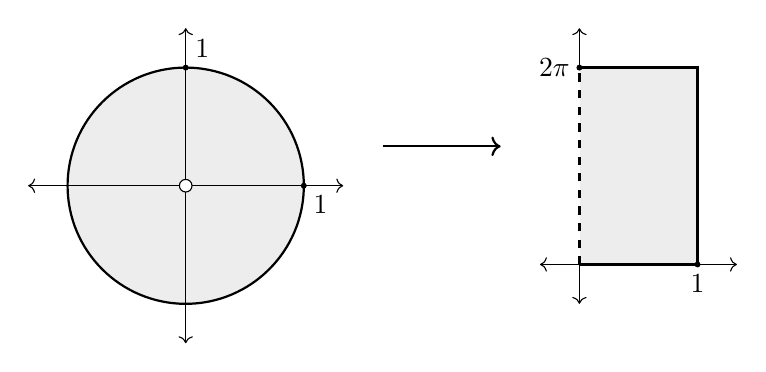
\begin{tikzpicture}
      \draw[thick, fill=lightgray] (0,0) circle (1.5); 
      \draw[<->] (-2,0)--(2,0);
      \draw[<->] (0,-2)--(0,2);
      \draw[fill=white] (0,0) circle (0.08);
      \draw[->, thick] (2.5,0.5)--(4, 0.5); 
      \draw[<->] (4.5,-1)--(7,-1);
      \draw[<->] (5,-1.5)--(5,2);
      \draw[white, fill=lightgray] (5,-1) rectangle (6.5,1.5);
      \draw[thick] (5,-1)--(6.5,-1)--(6.5,1.5)--(5,1.5);
      \draw[thick, dashed] (5,-1)--(5,1.5);
      \draw[fill] (6.5,-1) circle (0.03);
      \node[below] at (6.5,-1) {$1$};
      \node[left] at (5,1.5) {$2 \pi$};
      \draw[fill] (5, 1.5) circle (0.03);
      \draw[fill] (1.5,0) circle (0.03);
      \draw[fill] (0,1.5) circle (0.03);
      \node[below right] at (1.5,0) {$1$};
      \node[above right] at (0,1.5) {$1$};
  \end{tikzpicture}
  \end{center}

  If we are given an unbounded region $D \subset \mathbb{R}^2$, we can first create a bounded region and expand that region using a limit to cover all of $D$. 


 
\section{Sequences of Functions}

\section{Multivarite Functions} 

\subsection{Continuity} 

\subsection{Frechet Derivative}



\section{Integration of Differential Forms}

\section{Exercises} 

\subsection{Group Like Structures}

  \begin{exercise}[Math 401 Spring 2025 Midterm 2]
    Listed. 
    \begin{enumerate}
      \item Let $G$ be a finite group with an even number of elements. Show that $G$ contains an element of order $2$. 
      \item Prove that a group of order $10$ contains an element of order $5$. 
    \end{enumerate}
  \end{exercise}
  \begin{solution}
    Listed. 
    \begin{enumerate}
      \item We know that $e^{-1} = e$, and so remove it from $G$. Then $G$ has an odd number of elements. Now as long as $G$ is nonempty, we can remove $a, a^{-1}$, resulting in an odd cardinality. Since $G$ is finite, this must terminate, and so there must be a case where $a = a^{-1} \implies \ord(a) = 2$. 
      \item Assume that there is no element of order $5$. Then from above it must contain an element of order $2$, and let us call it $a \in G$. $\ord(e) = 1$ obviously. If any $b \in G$ had order 10, then $G = Z_{10}$, which would mean that $\ord(b^5) = 2$. Therefore every element other than the identity must have order $2$. But then given $a, b, ab \in G$, $ab \neq a, b$ since $ab = a \implies b = e$, and this is precisely the Klein 4 group. This subgroup has an order that doesn't divide 10, contradicting Lagrange's theorem. 
    \end{enumerate}
  \end{solution}

  \begin{exercise}[Shifrin 6.1.1]
    Which of the following are groups?
    \begin{enumerate}
      \item[(a)] $\{1,3,7,9\} \subset \mathbb{Z}_{10}$, with operation multiplication
      \item[(b)] $\{0,2,4,6\} \subset \mathbb{Z}_{10}$, with operation addition
      \item[(c)] $\{x \in \mathbb{Q} : 0 < x \leq 1\}$, with operation multiplication
      \item[(d)] the set of all positive irrational real numbers, with operation multiplication
      \item[(e)] the set of imaginary numbers $ix, x \in \mathbb{R}$, with operation addition
      \item[(f)] the set of complex numbers of modulus 1, with operation multiplication
      \item[(g)] $\mathbb{Z}$ with operation $a \bullet b = a + b + 1$
      \item[(h)] $\mathbb{Z}$ with operation $a \bullet b = a - b$
      \item[(i)] $\mathbb{Q} - \{1\}$ with operation $a \bullet b = a + b - ab$
    \end{enumerate}
  \end{exercise}
  \begin{solution}
    Listed. We will denote the sets in question to be $G$. 
    \begin{enumerate}
      \item[(a)] Is a group since product of 2 odds is odd, so is closed. Also we have $1$ as the identity with $3^{-1} = 7, 7^{-1} = 3, 9^{-1} = 9$. It is associative since multiplication on $\mathbb{Z}_{10}$ is associative. 
      \item[(b)] Not a group since $4 + 4 = 8 \not\in G$. 
      \item[(c)] Not a group since $1/2 \in G$ but $(1/2)^{-1} = 2 \not\in G$. 
      \item[(d)] Not a group since $\sqrt{2} \times \sqrt{2} 2  \not\in G$. 
      \item[(e)] Is a group since identity is $0 = 0i$, $ix + iy = i (x + y)$ with $x + y \in \mathbb{R}$, and $-(ix) = i (-x)$ where $-x \in \mathbb{R}$. 
      \item[(f)] Is a group since this is a representation of $O(2)$. 
      \item[(g)] Is a group since this is obviously closed under $\mathbb{Z}$ since $+_{\mathbb{Z}}$ is closed. Now assume that $i$ is the identity. Then $a \bullet i = a + i + 1 = a \implies i = -1$. Therefore $a \bullet a^{-1} = a + a^{-1} + 1 = -1 \implies a^{-1} = -a - 2$. This is associative since 
      \begin{equation}
        (a \bullet b) \bullet c = (a + b + 1) \bullet c = a + b + c + 2 = a \bullet (b + c + 1) = a \bullet (b \bullet c)
      \end{equation}
      \item[(h)] Not a group since it is not associative. Note $(a \bullet b) \bullet c = (a - b) \bullet c = a - b - c$, while $a \bullet (b \bullet c) = a \bullet (b - c) = a - b + c$. 
      \item[(i)] Is a group. We claim that it is closed. Assume not; given $a, b \neq 1$, 
        \begin{equation}
          a \bullet b = a + b - ab = 1 \implies 0 = ab - a - b + 1 = (a - 1)(b-1) 
        \end{equation}
        which means $a = 1$ or $b = 1$, which is a contradiction. As for the identity, $a \bullet i = a + i - ai = a \implies 0 = i - ai = i (1 - a) \implies i = 0$ since $a \neq 1$. We can define the inverse by solving 
        \begin{equation}
          0 = a \bullet a^{-1} = a + a^{-1} - a a^{-1} \implies a^{-1} (1 - a) = -a \implies a^{-1} = \frac{a}{a-1}
        \end{equation}
        which is well-defined since $a \neq 1$. Finally, it is associative since 
        \begin{align}
          (a \bullet b) \bullet c & = (a + b - ab) \bullet c \\
                                  & = a + b - ab + c - ac - bc - abc \\
                                  & = a + b + c - bc - ab - ac - abc \\
                                  & = a \bullet (b + c - bc) \\
                                  & = a \bullet (b \bullet c)
        \end{align}
    \end{enumerate}
  \end{solution}

  \begin{exercise}[Shifrin 6.1.10]
    \begin{enumerate}
      \item[(a)] Let $G$ be a group. Prove that $(ab)^2 = a^2b^2$ for all $a,b \in G$ if and only if $G$ is abelian.
      \item[(b)] Prove that if every element (other than the identity element) of a group $G$ has order 2, then $G$ is abelian.
    \end{enumerate}
  \end{exercise}
  \begin{solution}
    For (a), if $G$ is abelian, then 
    \begin{equation}
      (ab)^2 = (ab) (ab) = a (ba) b = a (ab) b = (aa) (bb) = a^2 b^2
    \end{equation}
    If the identity holds, then 
    \begin{equation}
      (ab)^2 = a^2 b^2 \implies (a^{-1} a) (ba) (b b^{-1}) = a^{-1} (ab)(ab) b^{-1} = a^{-1} a^2 b^2 b^{-1} \implies ba = ab
    \end{equation} 
    For (b), since we have $a^2 = e, b^2 = e$, and $(ab)^2 = e$, from (a) $G$ is abelian. 
  \end{solution}

  \begin{exercise}[Shifrin 6.1.17]
    \begin{enumerate}
      \item[(a)] A group has four elements $a$, $b$, $c$, and $d$, subject to the rules $ca = a$ and $d^2 = a$. Fill in the entire multiplication table at the left below.
      
      \begin{tabular}{c|cccc}
        $\cdot$ & $a$ & $b$ & $c$ & $d$ \\
        \hline
        $a$ & & & & \\
        $b$ & & & & \\
        $c$ & $a$ & & & \\
        $d$ & & & & $a$ \\
      \end{tabular}
      
      \item[(b)] A group has six elements $a$, $b$, $c$, $d$, $e$, and $f$, subject to the rules $ae = a$, $bd = a$, $c^2 = a$, and $df = a$. Fill in the entire multiplication table at the right above.
      
      \begin{tabular}{c|cccccc}
        $\cdot$ & $a$ & $b$ & $c$ & $d$ & $e$ & $f$ \\
        \hline
        $a$ & & & & & $a$ & \\
        $b$ & & & & $a$ & & \\
        $c$ & & & $a$ & & & \\
        $d$ & & & & & & $a$ \\
        $e$ & & & & & & \\
        $f$ & & & & & & \\
      \end{tabular}
    \end{enumerate}
  \end{exercise}
  \begin{solution}
    We can see that $ca = a \implies c = ca a^{-1} = a a^{-1} = i$, so $c$ is the identity. We can fill in the row and column of $c$. Then, we can figure out what $bd$ is. It cannot be $b$ or $d$ since $c$ is the unique identity, so it must be either $a$ or $c$. It cannot be $a$ since then $bd = a = d^2$, and so $b = d$. So it must be $c$. By the same logic we can fill out the rest of the rows and columns. 

    \begin{tabular}{c|cccc}
      $\cdot$ & $a$ & $b$ & $c$ & $d$ \\
      \hline
      $a$ & $c$ & $d$ & $a$ & $b$ \\
      $b$ & $d$ & $a$ & $b$ & $c$ \\
      $c$ & $a$ & $b$ & $c$ & $d$ \\
      $d$ & $b$ & $c$ & $d$ & $a$ \\
    \end{tabular}

    By the same logic as the previous, we can immediately see that $ae = a \implies e$ is the identity. The formal logic above can be simplified down to saying that there can be no two of the same elements in the same row or column, since if it were, then we are saying that $xy = xz \implies y = z$, which cannot be the case since $y$ and $z$ are distinct. So $fb = a$. We can also deduce that $da = ab$ and $ba = af$. At this point, we can recognize that this is the Dihedral group of order $6$, and so we fill in the rest of the multiplication table. 

    \begin{tabular}{c|cccccc}
      $\cdot$ & $a$ & $b$ & $c$ & $d$ & $e$ & $f$ \\
      \hline
      $a$ & c & f & e & b & a & d \\
      $b$ & d & e & f & a & b & c \\
      $c$ & e & d & a & f & c & b \\
      $d$ & f & c & b & e & d & a \\
      $e$ & a & b & c & d & e & f \\
      $f$ & b & a & d & c & f & e
    \end{tabular}
  \end{solution}

\subsection{Subgroups and Quotient Groups}

  \begin{exercise}[Shifrin 6.2.2]
    Prove that $\mathbb{Z}_7^{\times} \cong \mathbb{Z}_6$. (It is crucial to remember that we multiply in $\mathbb{Z}_7^{\times}$ and add in $\mathbb{Z}_6$.)
  \end{exercise}
  \begin{solution}
    Both groups are of order 6, and so $\mathbb{Z}_7^\times$---which is indeed a group (since it is the group of units of the ring $(\mathbb{Z}_7, +, \times)$)---must be isomorphic to either $\mathbb{Z}_6$ or $S_3$. However, $S_3$ is not abelian, while $\mathbb{Z}^\times_7$ is, so it must be the case that it is isomorphic to $\mathbb{Z}_6$. 
  \end{solution}

  \begin{exercise}[Shifrin 6.2.15.a/b]
    The \textbf{dihedral group} of order $2n$, denoted $\mathcal{D}_n$, is given by $\{\rho^i\psi^j : 0 \leq i < n, 0 \leq j \leq 1\}$ subject to the rules $\rho^n = e$, $\psi^2 = e$, and $\psi\rho\psi^{-1} = \rho^{-1}$.
    \begin{enumerate}
      \item Check this is really a group. That is, what is $(\rho^i\psi^j)^{-1}$, and what is the product $(\rho^i\psi^j)(\rho^k\psi^\ell)$?
      \item Check that $\mathcal{T} \cong \mathcal{D}_3$ and $S_q \cong \mathcal{D}_4$.
    \end{enumerate}
  \end{exercise}
  \begin{solution}
    We check the properties of a group. The following identity is useful: 
    \begin{equation}
      (\psi \rho \psi^{-1})^{n-i} = (\rho^{-1})^{n-i} \implies \psi \rho^{n-i} \psi^{-1} = \rho^i \implies \psi \rho^{n-i} = \rho^i \psi
    \end{equation}
    \begin{enumerate}
      \item \textit{Closure}. From simplifying according to the first two rules, we will automatically adjust the exponents to be $i, k < n$ (by subtracting out multiples of $n$) and $j \in \{0, 1\}$ (by subtracting out multiples of $2$). Going case by case, 
      \begin{enumerate}
        \item $j = 0, l = 0$. $\rho^i \rho^k = \rho^{i+k}$. 
        \item $j = 0, l = 1$. $\rho^i \rho^k \psi = \rho^{i+k} \psi$. 
        \item $j = 1, l = 0$. $\rho^i \psi \rho^k = \rho^i \rho^{n-k} \psi = \rho^{n-k+i} \psi$. 
        \item $j = 1, l = 1$. $\rho^i \psi \rho^k \psi = \rho^i \psi \psi \rho^{n-k} = \rho^i \rho^{n-k} = \rho^{n-k+i}$. 
      \end{enumerate}
      \item \textit{Identity}. The identity is $e = \rho^0 \psi^0$. We can see that $e \rho^i \psi^j = \rho^i \psi^j e = \rho^{i+0} \psi^j$. 
      \item \textit{Inverse}. We have $\psi \rho \psi^{-1} = \psi \rho \psi = \rho^{-1} \implies \psi \rho = \rho^{-1} \psi^{-1} = (\psi \rho)^{-1}$. Therefore, 
      \begin{equation}
        (\rho^i \psi^j)^{-1} = \begin{cases} 
          \rho^{n - i} & \text{ if } j = 0  \\
          \rho^{i} \psi & \text{ if } j = 1
        \end{cases}
      \end{equation}
      which are both of the correct form and therefore in $\mathcal{D}_n$. To verify, we see that $\rho^i \rho^{n-i} = \rho^n = e$, and $(\rho^i \psi) (\rho^i \psi) = \rho^i \psi \psi \rho^{n-i} = \rho^i \rho^{n-i} = e$.  
      \item \textit{Associativity}. Can also be proven tediously but problem only asked to state the product and inverse.  
    \end{enumerate} 

    For (b) for $\mathcal{T}$, we can explicitly look at the multiplication tables and see that they are isomorphic. We denote $r_1, r_2$ as the 120 and 240 degree rotations, and $f_1, f_2, f_3$ as the flips across each axis. 

    \begin{figure}[H]
      \centering
      \begin{subfigure}[b]{0.48\textwidth}
        \centering
        \begin{tabular}{c|cccccc}
          & $e$ & $\rho$ & $\rho^2$ & $\psi$ & $\rho\psi$ & $\rho^2\psi$ \\
          \hline
          $e$ & $e$ & $\rho$ & $\rho^2$ & $\psi$ & $\rho\psi$ & $\rho^2\psi$ \\
          $\rho$ & $\rho$ & $\rho^2$ & $e$ & $\rho^2\psi$ & $\psi$ & $\rho\psi$ \\
          $\rho^2$ & $\rho^2$ & $e$ & $\rho$ & $\rho\psi$ & $\rho^2\psi$ & $\psi$ \\
          $\psi$ & $\psi$ & $\rho^2\psi$ & $\rho\psi$ & $e$ & $\rho^2$ & $\rho$ \\
          $\rho\psi$ & $\rho\psi$ & $\psi$ & $\rho^2\psi$ & $\rho$ & $e$ & $\rho^2$ \\
          $\rho^2\psi$ & $\rho^2\psi$ & $\rho\psi$ & $\psi$ & $\rho^2$ & $\rho$ & $e$
        \end{tabular}
        \caption{$\mathcal{D}_3$}
      \end{subfigure}
      \hfill 
      \begin{subfigure}[b]{0.48\textwidth}
        \centering
        \begin{tabular}{c|cccccc}
          & $e$ & $r_1$ & $r_2$ & $f_1$ & $f_2$ & $f_3$ \\
          \hline
          $e$ & $e$ & $r_1$ & $r_2$ & $f_1$ & $f_2$ & $f_3$ \\
          $r_1$ & $r_1$ & $r_2$ & $e$ & $f_3$ & $f_1$ & $f_2$ \\
          $r_2$ & $r_2$ & $e$ & $r_1$ & $f_2$ & $f_3$ & $f_1$ \\
          $f_1$ & $f_1$ & $f_2$ & $f_3$ & $e$ & $r_2$ & $r_1$ \\
          $f_2$ & $f_2$ & $f_3$ & $f_1$ & $r_1$ & $e$ & $r_2$ \\
          $f_3$ & $f_3$ & $f_1$ & $f_2$ & $r_2$ & $r_1$ & $e$
        \end{tabular}
        \caption{$\mathcal{T}$}
      \end{subfigure}
    \end{figure}

    For $S_q$, it is tedious to write the full table, so we construct the isormorphisms using the generators. For $S_q$, the symmetry group of the square consists of 8 elements: the 4 rotations $r_1, r_2, r_3, r_4$ (of 90, 180, 270, and 360=0 degrees), and the flips $f_1, f_2, f_3, f_4$ (across each axis). Now we construct the function $g: \mathcal{D}_3 \rightarrow \mathcal{T}$ such that $f(\rho) = r_1$ and $f(\psi) = f_1$. Then we can see that 
    \begin{equation}
      g(\rho^4) = g(e) = e = r_1^4 = g(\rho^4), \qquad g(\psi^2) = g(e) = e = f_1^2 = g(\psi)^2
    \end{equation}
    since 90 degrees rotated 4 times is $0$ degrees, the identity, and two flips across the same axis is also the identity. Finally, we have 
    \begin{equation}
      g(\psi \rho \psi) = g(\rho^{-1}) = r_1^{-1} = r_3 = f_1 r_1 f_1 = g(\psi) g(\rho) g(\psi)
    \end{equation}
    Where $r_1^{-1} = r_3$ since a rotation of 270 after a 90 is the same as rotation by 360=0, and $r_3 = f_1 r_1 f_1$ is the change of basis symmetry observed in Shifrin Example 6.1.5. Therefore the rules match, making it a homomorphism, and since the order is the same ($\mathcal{D}_3$ has $4 \times 2 = 8$ elements from looking at the indices), this is an isomorphism. 
  \end{solution}

  \begin{exercise}[Shifrin 6.3.8]
    Let $H \subset G$ be a subgroup, and let $a \in G$ be given. Prove that $aHa^{-1} \subset G$ is a subgroup (called a \textbf{conjugate subgroup} of $H$). Prove, moreover, that it is isomorphic to $H$ (cf. Exercise 6.2.12).
  \end{exercise}
  \begin{solution}
    Let $x, y \in aHa^{-1}$. Then $x = a h_x a^{-1}, y = a h_y a^{-1}$ for some $h_x, h_y \in H$. Therefore, 
    \begin{enumerate}
      \item It is closed. $xy = (a h_x a^{-1}) (a h_y a^{-1}) = a h_x (a^{-1} a) h_y a^{-1} = a h_x h_y a^{-1} \in aHa^{-1}$ since $h_x h_y \in H$ by closure. 
      \item It has an identity since $e \in H \implies a e a^{-1} = a a^{-1} = e \in aHa^{-1}$. 
      \item It has inverses since given $x \in H$ as above with inverses $x^{-1}$, we see that $(a x a^{-1})^{-1} = (a^{-1})^{-1} x^{-1} a^{-1} = a x^{-1} a^{-1} \in a H a^{-1}$ since $x^{-1} \in H$ by $H$ being a group. 
      \item Associativity is inherited from $G$. 
    \end{enumerate} 
    It suffices to show that this is injective, since the map $\iota : H \rightarrow a H a^{-1}$ is surjective by definition. Given $x, y \in a H a^{-1}$ with $x = y$, we have $a h_x a^{-1} = a h_y a^{-1}$, and multiplying by $a$ on the right and then $a^{-1}$ on the left, we get $h_x = h_y$.
  \end{solution}

  \begin{exercise}[Shifrin 6.3.11]
    Prove that a group of order $n$ has a proper subgroup if and only if $n$ is composite.
  \end{exercise}
  \begin{solution}
    We prove bidirectionally. Call the group $G$ and subgroup $H$. 
    \begin{enumerate}
      \item $(\rightarrow)$. Assume $n$ is prime. Then by Lagrange's theorem $|H|$ must divide $n$, and so $|H| = 1$ or $n$, neither of which results in a proper subgroup. 
      \item $(\leftarrow)$. Assume $G$ has a proper subgroup $H$. Since it is proper, $|H| \neq 1, n$. Then by Lagrange's theorem, $|H|$ divides $n$, which implies that $n$ is composite. 
    \end{enumerate}
  \end{solution}

  \begin{exercise}[Shifrin 6.3.13]
    Suppose $H, K \subset G$ are subgroups of orders $5$ and $8$, respectively. Prove that $H \cap K = \{e\}$.
  \end{exercise}
  \begin{solution}
    Let us take an arbitrary element in $x \in H \cap K$ and consider the cyclic group $\langle x \rangle$. By Lagrange's Theorem, the order $|x|$ in $H$ must be either $1$ or $5$, while the order in $K$ must be $1, 2, 4, 8$. Therefore, $|x| = 1$ and so $x = e$. 
  \end{solution}

  \begin{exercise}[Shifrin 6.3.17]
    \begin{enumerate}
      \item Prove that a group $G$ of even order has an element of order $2$. (Hint: If $a \neq e$, $a$ has order $2$ if and only if $a = a^{-1}$.)
      \item Suppose $m$ is odd, $|G| = 2m$, and $G$ is abelian. Prove $G$ has precisely one element of order $2$. (Hint: If there were two, they would provide a Klein four-group.)
      \item Prove that if $G$ has exactly one element of order $2$, then it must be in the center of $G$.
    \end{enumerate}
  \end{exercise}
  \begin{solution}
    Listed. 
    \begin{enumerate}
      \item Assume the contrary and take $H = G \setminus \{e\}$. Then $|H|$ is odd, and since no element has order $2$, every element must be associated with a unique inverse $a, a^{-1}$. But this cannot happen since $|H|$ is odd. Therefore there must be at least one element of order $2$. 

      \item It has at least 1 element of order 2 from (1). Now assume that there are two, call them $a, b$. Then $ab \neq a, b$ and $ab$ also has order $2$ since $(ab)(ab) = abba = aa = e$. Therefore, calling $c = ab$, we have $ac = ca = aab = b$ and $bc = cb = abb = a$. This fully defines the multiplication table for the Klein 4 group $K$ of order $4$. Therefore, by Lagrange's theorem, we have found a subgroup $K$ and so $|K|$ must divide $G$. However, this would mean that $m$ must be even, a contradiction. Therefore there is only one such unique $a$. 

      \item Given $a \in G$ with $|a| = 2$, we wish to show that it is an element of $Z = \{ b \in G \mid bx = xb \forall x \in G\}$.\footnote{I am using the definition of center defined in Shifrin 6.3.7.} Consider $z = x^{-1} a x$. We have 
      \begin{equation}
        z^2 = (x^{-1} a x)^2 = x^{-1} a x x^{-1} a x = x^{-1} a^2 x = x^{-1} x = e
      \end{equation}
      which means that $z$ also has order $2$. But since this is unique, it must be that $z = a$. Therefore, by multiplying $x$ on the left, we get 
      \begin{equation}
        x^{-1} a x = a \implies ax = xa
      \end{equation}
    \end{enumerate}
  \end{solution}
  
  \begin{exercise}[Assigned]
    Find all group homomorphisms $\mathbb{Z}_n \to \mathbb{Z}_m$. (Your answer will depend on $n$ and $m$.) 
  \end{exercise}
  \begin{solution}
    Given a homomorphism, $f$, we must have $f(0) = 0$. Let $f(1) = k$. Note that the value of $f(1) = k$ completely determines the homomorphism since the image of every other $l \in \mathbb{Z}_n$ is defined by 
    \begin{equation}
      f(l) = f(\underbrace{1 + \ldots + 1}_{l \text{ times}}) = \underbrace{k + \ldots + k}_{l \text{ times}}
    \end{equation}
    Since the image of $f$ must be a cyclic subgroup of $\mathbb{Z}_m$, we must satisfy 
    \begin{align}
      0 = f(0) & = f(\underbrace{1 + \ldots + 1}_{n \text{ times}}) \\
               & = \underbrace{k + \ldots + k}_{n \text{ times}} 
    \end{align}
    and so $m \mid nk$. Therefore, $k$ must be a multiple of $m/\gcd(n, m)$. So all homomorphisms are determined by the set 
    \begin{equation}
      \bigg\{ k = \frac{a m}{\gcd(n, m)} \; \bigg| \; a \in \mathbb{N}, 0 \leq k \leq m-1 \bigg\}
    \end{equation}
    which we can see ranges from $0 \leq a < \gcd(n, m)$, and so the total number of homomorphisms is $\gcd(n, m)$. Note that there is always the trivial homomorphism when $a = 0$, i.e. everything maps to $0$. For example, if we have $f: \mathbb{Z}_{14} \to \mathbb{Z}_{21}$, we have $k = 0, 3, 6, 9, 12, 15, 18$. 
  \end{solution}

\subsection{Group Actions}

\subsection{Product Groups}

\subsection{Ring Like Structures}

  \begin{exercise}[Shifrin 1.2.1]
    For each of the following pairs of numbers $a$ and $b$, find $d = \gcd(a,b)$ and express $d$ in the form $ma+nb$ for suitable integers $m$ and $n$.
    \begin{enumerate}
      \item[(a)] $14, 35$
      \item[(b)] $56, 77$
      \item[(c)] $618, 336$
      \item[(d)] $2873, 6643$
      \item[(e)] $512, 360$
      \item[(f)] $4432, 1080$
    \end{enumerate}
  \end{exercise}
  \begin{solution}
    Listed. 
    \begin{enumerate}
      \item $d = 7 = (-2) \cdot 14 + (1) \cdot 35$. 
      \item $d = 7 = (-4) \cdot 56 + 3 \cdot 77$. 
      \item $d = 6 = -25 \cdot 618 + 46 \cdot 336$ 
      \item $d = 13 = 37 \cdot 2873 + (-16) \cdot 6643$. 
      \item $d = 8 = 19 \cdot 512 + (-27) \cdot 360$. 
      \item $d = 8 = 29 \cdot 4432 + (-119) \cdot 1080$. 
    \end{enumerate}
  \end{solution}

  \begin{exercise}[Shifrin 1.2.2]
    You have at your disposal arbitrarily many 4-cent stamps and 7-cent stamps. What are the postages you can pay? Show in particular that you can pay all postages greater than 17 cents.
  \end{exercise}

  \begin{exercise}[Shifrin 1.2.3]
    Prove that whenever $m \neq 0$, $\gcd(0, m) = |m|$.
  \end{exercise}

  \begin{exercise}[Shifrin 1.2.4]
    \begin{enumerate}
      \item[(a)] Prove that if $a|x$ and $b|y$, then $ab|xy$.
      \item[(b)] Prove that if $d = \gcd(a, b)$, then $\gcd(\frac{a}{d}, \frac{b}{d}) = 1$.
    \end{enumerate}
  \end{exercise}

  \begin{exercise}[Shifrin 1.2.5]
    Prove or give a counterexample: the integers $q$ and $r$ guaranteed by the division algorithm, Theorem 2.2, are unique.
  \end{exercise}

  \begin{exercise}[Shifrin 1.2.6]
     Prove or give a counterexample. Let $a, b \in \mathbb{Z}$. If there are integers $m$ and $n$ so that $d = am + bn$, then $d = \gcd(a, b)$.
  \end{exercise}

  \begin{exercise}[Shifrin 1.2.7]
    Generalize Proposition 2.5: if $\gcd(m, c) = 1$ and $m|cz$, then prove $m|z$.
  \end{exercise}
  \begin{solution}
    Let $\mathrm{gcd}(m, c) = 1$ and $m | cz$. Then there exists $a, b \in \mathbb{Z}$ such that $am + bc = 1$. Multiply both sides of the equation by $z$ to get by the distributive property 
    \begin{equation}
      (am + bc) z = amz + bcz = z
    \end{equation} 
    $m | amz$ and $m | cz \implies m | bcz$. Therefore, the sum of the two, which is equal to $z$, must be divisible by $m$. Therefore $m | z$. 
  \end{solution}

  \begin{exercise}[Shifrin 1.2.8]
    Suppose $a, b, n \in \mathbb{N}$, $\gcd(a, n) = 1$, and $\gcd(b, n) = 1$. Prove or give a counterexample: $\gcd(ab, n) = 1$.
  \end{exercise}

  \begin{exercise}[Shifrin 1.2.9]
    Prove that if $p$ is prime and $p|(a_1 a_2 \ldots a_n)$, then $p|a_j$ for some $j$, $1 \leq j \leq n$. (Hint: Use Proposition 2.5 and induction.)
  \end{exercise}

  \begin{exercise}[Shifrin 1.2.10]
    Given a positive integer $n$, find $n$ consecutive composite numbers.
  \end{exercise}

  \begin{exercise}[Shifrin 1.2.11]
    Prove that there are no integers $m, n$ so that $(\frac{m}{n})^2 = 2$. (Hint: You may start by assuming $m$ and $n$ are relatively prime. Why? Then use Exercise 1.1.3.)
  \end{exercise}

  \begin{exercise}[Shifrin 1.2.12]
    Find all rectangles whose sides have integral lengths and whose area and perimeter are equal.
  \end{exercise}

  \begin{exercise}[Shifrin 1.2.13]
    Given two nonzero integers $a, b$, in analogy with the definition of $\gcd(a, b)$, we define the \textbf{least common multiple} $\operatorname{lcm}(a, b)$ to be the positive number $\mu$ with the properties:
    \begin{enumerate}
      \item[(i)] $a|\mu$ and $b|\mu$, and
      \item[(ii)] if $s \in \mathbb{Z}$, $a|s$ and $b|s \Rightarrow \mu|s$.
    \end{enumerate}
    Prove that
    \begin{enumerate}
      \item[(a)] if $\gcd(a, b) = 1$, then $\mu = ab$. (Hint: If $\gcd(a, b) = 1$, then there are integers $m$ and $n$ so that $1 = ma + nb$; therefore, $s = mas + nbs$.)
      \item[(b)] more generally, if $\gcd(a, b) = d$, then $\mu = ab/d$.
    \end{enumerate}
  \end{exercise}
  \begin{solution}
    Listed. 
    \begin{enumerate}
      \item We can simply verify the two properties. Since $\mu = ab$, $a | \mu$ and $b | \mu$ trivially by the existence of $b$ and $a$, respectively. As for the second property, let $s \in \mathbb{Z}$ exist such that $a | s$ and $b | s$. Since $a | s$, $s = xa$ for some $x \in \mathbb{Z}$. But since $b | s$, $b | xa$. Since $\mathrm{gcd}(a, b) = 1$ by assumption, the result in [Shifrin 1.2.7] tells us that $b | x$, i.e. there exists some $k \in \mathbb{Z}$ such that $x = kb$. Therefore $s = xa = kba = kab = k \mu$. By existence of $k$, $\mu | s$, and we are done. 
      \item Given $a, b$ with $\mathrm{gcd}(a, b) = d$, there exists some $a^\prime, b^\prime \in \mathbb{Z}$ s.t. $a = da^\prime, b = db^\prime$. We claim that $\mu = ab/d \coloneqq d a^\prime b^\prime$ is the lcm.\footnote{Since division isn't generally closed in the integers, I prefer to define $ab/d$ this way.} It is clear that $a | \mu$ and $b | \mu$ by the existence of integers $b^\prime$ and $a^\prime$, respectively. To prove the second property, let $s \in \mathbb{Z}$ with $a | s$ and $b | s$. Since $a | s \iff d a^\prime | s$, there must exist some $x \in \mathbb{Z}$ s.t. $s = d a^\prime x$. But since $b | s$, this means that $d b^\prime | s \iff d b^\prime | d a^\prime x \iff b^\prime | a^\prime x$. But $\mathrm{gcd}(a^\prime, b^\prime) = 1$ which follows from the definition of gcd, and so by [Shifrin 1.2.7] it must be the case that $b^\prime | x$, i.e. there exists some $k \in \mathbb{Z}$ s.t. $x = b^\prime k$. Substituting this back we have $s = d a^\prime b^\prime k = \mu k$, and by existence of $k$ it follows that $\mu | s$. Since it satisfies these 2 properties $\mu$ is the lcm. 
    \end{enumerate}
  \end{solution} 

  \begin{exercise}[Shifrin 1.2.14]
    See Exercise 13 for the definition of $\operatorname{lcm}(a, b)$. Given prime factorizations $a = p_1^{\mu_1} \cdots p_m^{\mu_m}$ and $b = p_1^{\nu_1} \cdots p_m^{\nu_m}$, with $\mu_i, \nu_i \geq 0$, express $\gcd(a, b)$ and $\operatorname{lcm}(a, b)$ in terms of $p_1,\ldots,p_m$. Prove that your answers are correct.
  \end{exercise}

  \begin{exercise}[Shifrin 1.3.8] 
    We see that in $\bmod{10}$, 
    \begin{align}
      3^{400} \equiv 9^{200} \equiv (-1)^{200} \equiv 1^{100} \equiv 1
    \end{align} 
    so the last digit is $1$. To get the last 2 digits, we use the binomial expansion and focus on the last 2 terms. 
    \begin{equation}
      3^{400} = 9^{200} = (10 - 1)^{200} = \ldots + \binom{200}{199} 10^1 (-1)^{199} + \binom{200}{200} (-1)^{200} 
    \end{equation}
    since every combination of the form $\binom{n}{k}$ is an integer and all the other terms have a factor of $10^2$, the expansion $\bmod{100}$ becomes 
    \begin{equation}
      3^{400} \equiv \binom{200}{199} 10^1 (-1)^{199} + \binom{200}{200} (-1)^{200} = 200 \cdot 10 \cdot (-1)^{199} + 1 \equiv 1 \pmod{100}
    \end{equation}
    and so the last two digits is $01$. To get the last digit of $7^{99}$, we see that in $\bmod{10}$, 
    \begin{equation}
      7^{99} \equiv 7^{96} \cdot 7^3 \equiv (7^4)^{24} \cdot 343 \equiv 2401^{24} \cdot 343 \equiv 1^{24} \cdot 3 \equiv 3
    \end{equation}
  \end{exercise}

  \begin{exercise}[Shifrin 1.3.10]
    We must show that 
    \begin{equation}
      n \equiv 0 \pmod{13} \iff n^\prime = \sum_{i=1}^k a_i 10^{i-1} + 4a_0 \equiv 0 \pmod{13}
    \end{equation} 
    We see that $n \equiv n + 39 a_0 \equiv 0 \pmod{13}$, and 
    \begin{align}
      n + 39 a_0 & = \sum_{i=0}^k 10^i a_i + 39 a_0 \\
                 & = \sum_{i=1}^k 10^i a_i + 40 a_0 \\
                 & = 10 \bigg( \sum_{i=1}^k 10^{i-1} a_i + 4 a_0 \bigg) \\
                 & = 10 n^\prime
    \end{align} 
    and so we have $n \equiv 10 n^\prime \pmod{13}$, and so $n^\prime \equiv 0 \pmod{13} \implies n \equiv 0 \pmod{13}$. Conversely, if $n \equiv 0 \pmod{13}$, then $4n \equiv 0 \pmod{13}$, but $4n \equiv 40 n^\prime$ and so $n^\prime \equiv 40 n^\prime \equiv 4n \equiv 0 \pmod{13}$. Therefore both implications are proven. 
  \end{exercise}

  \begin{exercise}[Shifrin 1.3.12]
    Suppose that $p$ is prime. Prove that if $a^2 \equiv b^2 \pmod{p}$, then $a \equiv b \pmod{p}$ or $a \equiv -b \pmod{p}$. 
  \end{exercise}
  \begin{solution}
    We have 
    \begin{align}
      a^2 \equiv b^2 \pmod{p} & \implies a^2 - b^2 \equiv 0 \pmod{p} \\
                              & \implies (a + b) (a - b) \equiv 0 \pmod{p}
    \end{align} 
    We claim that there are no zero divisors in $\mathbb{Z}_p$. If $mn \equiv 0 \pmod{p}$, then by definition this means $p | mn$, which implies that in the integers this must mean that $p | m$ or $p | n$.\footnote{Proposition 2.5} But since $m, n \not\equiv 0$, $p \not| n$ and $p \not| m$, arriving at a contradiction. Going back to our main argument, it must be the case that $a + b \equiv 0 \implies a \equiv -b$ or $a - b \equiv 0 \implies a \equiv b$.  
  \end{solution}

  \begin{exercise}[Shifrin 1.3.15]
    Let us assume that $n = a^2 + b^2 + c^2$ for some $a, b, c \in \mathbb{Z}$. Let us consider for each integer $z$, all the possible values of $z^2 \pmod{8}$. 
    \begin{align}
      z \equiv 0 & \implies z^2 \equiv 0 \pmod{8} \\
      z \equiv 1 & \implies z^2 \equiv 1 \pmod{8} \\
      z \equiv 2 & \implies z^2 \equiv 4 \pmod{8} \\
      z \equiv 3 & \implies z^2 \equiv 1 \pmod{8} \\
      z \equiv 4 & \implies z^2 \equiv 0 \pmod{8} \\
      z \equiv 5 & \implies z^2 \equiv 1 \pmod{8} \\
      z \equiv 6 & \implies z^2 \equiv 4 \pmod{8} \\
      z \equiv 7 & \implies z^2 \equiv 1 \pmod{8} 
    \end{align}
    Therefore, $a^2 + b^2 + c^2 \pmod{8}$ can take any values of the form 
    \begin{equation}
      x + y + z \pmod{8} \text{ for } x, y, z \in \{0, 1, 4\}
    \end{equation}
    Since addition is commutative, WLOG let $x \leq y \leq z$. We can just brute force search this. 
    \begin{enumerate}
      \item If $z = 0$, then $x = y = z = 0$ and $x + y + z = 0 \not\equiv 7$. 
      \item If $z = 1$, then we see 
      \begin{align}
        0 + 0 + 1 \equiv 1 \\ 
        0 + 1 + 1 \equiv 2 \\ 
        1 + 0 + 1 \equiv 2 \\ 
        1 + 1 + 1 \equiv 3 
      \end{align}
      \item If $z = 4$, then we see that 
        \begin{align}
          0 + 0 + 4 & \equiv 4 \\
          0 + 1 + 4 & \equiv 5 \\
          0 + 4 + 4 & \equiv 0 \\
          1 + 1 + 4 & \equiv 6 \\
          1 + 4 + 4 & \equiv 1 \\
          4 + 4 + 4 & \equiv 4
        \end{align}
    \end{enumerate}
    And so $a^2 + b^2 + c^2 \not\equiv 7 \pmod{8}$ for any $a, b, c \in \mathbb{Z}$. 
  \end{exercise}

  \begin{exercise}[Shifrin 1.3.20.a/b/g]
    For (a), 
    \begin{equation}
      3x \equiv 2 \pmod{5} \implies 6x \equiv 4 \pmod{5} \implies x \equiv 4 \pmod{5} 
    \end{equation}
    For (b), 
    \begin{align}
      6x + 3 \equiv 1 \pmod{10} & \implies 6x \equiv -2 \equiv 8 \pmod{10} \\
                                & \implies 10 | (6x - 8) \\
                                & \implies 5 | (3x - 4) \\
                                & \implies 3x \equiv 4 \pmod{5} \\
                                & \implies 3x \equiv 9 \pmod{5} \\
                                & \implies x \equiv 3 \pmod{5}
    \end{align}
    For (g), 
    \begin{align}
      15x \equiv 25 \pmod{35} & \implies 35 | (15x - 25) \\
                              & \implies 7 | (3x - 5) \\
                              & \implies 3x \equiv 5 \pmod{7} \\
                              & \implies 3x \equiv 12 \pmod{7} \\ 
                              & \implies x \equiv 4 \pmod{7}
    \end{align}
  \end{exercise}

  \begin{exercise}[Shifrin 1.3.21.b/c]
    For (b), we see that $4$ and $13$ are coprime with $-3 \cdot 4 + 1 \cdot 13 = 1$. Therefore, by the Chinese remainder theorem 
    \begin{equation}
      x \equiv 1 \cdot 1 \cdot 12 + (-3) \cdot 7 \cdot 4 \pmod{52} \implies x \equiv 33 \pmod{52}
    \end{equation}
    For (c), we solve the first two congruences $x \equiv 3 \pmod{4}$ and $x \equiv 4 \pmod{5}$. $4$ and $5$ are coprime with $-1 \cdot 4 + 1 \cdot 5 = 1$. Therefore, by CRT 
    \begin{equation}
      x \equiv -1 \cdot 4 \cdot 4 + 1 \cdot 5 \cdot 3 \pmod{20} \implies x \equiv -1 \pmod{20}
    \end{equation}
    Then we solve $x \equiv -1 \pmod{20}$ with the final congruence $x \equiv 3 \pmod{7}$. We see that $20$ and $7$ are coprime with $-1 \cdot 20 + 3 \cdot 7 = 1$. Therefore by CRT 
    \begin{equation}
      x \equiv -1 \cdot 20 \cdot 3 + 3 \cdot 7 \cdot -1 \pmod{140} \implies x \equiv 59 \pmod{140}
    \end{equation}
  \end{exercise}

  \begin{exercise}[Shifrin 1.3.25]
    We prove bidirectionally. 
    \begin{enumerate}
      \item Assume a solution exists for $cx \equiv b \pmod{m}$. Then $m | (cx - b)$, which means that there exists a $y \in \mathbb{Z}$ s.t. $my = cx - b \iff b = cx - my$. Since $d = \mathrm{gcd}(c, m)$, there exists $c^\prime, m^\prime \in \mathbb{Z}$ s.t. $c = d c^\prime$ and $m = d m^\prime$. So 
      \begin{equation}
        b = cx - my = d (c^\prime x - m^\prime y) \implies d | b
      \end{equation} 

    \item Assume that $d | b$. Then there exists a $b^\prime \in \mathbb{Z}$ s.t. $b = d b^\prime$, and we have 
    \begin{align}
      cx \equiv b \pmod{m} & \iff m | (cx - b) \\
                           & \iff d m^\prime | d (c^\prime x - b^\prime) \\
                           & \iff m^\prime | (c^\prime x - b^\prime) \\
                           & \iff c^\prime x \equiv b^\prime \pmod{m^\prime} 
    \end{align}
    Since $\mathrm{gcd}(c^\prime, m^\prime) = 1$\footnote{Since $\mathrm{gcd}(c, m) = d \implies$ that there exists a $y, z \in \mathbb{Z}$ s.t. $c y + m z = d$, and dividing both sides by $d$ guarantees the existence of $y, z$ satisfying $c^\prime y + m^\prime z = 1$, meaning that $\mathrm{gcd}(c^\prime, m^\prime) = 1$.}, by Shifrin Proposition 3.5 the equation $c^\prime x \equiv b^\prime \pmod{m^\prime}$ is guaranteed to have a solution, and working backwards in the iff statements gives us the solution for $cx \equiv b \pmod{m}$. 
    \end{enumerate}

    We have proved existence of a solution in $\bmod{(m/d) = m^\prime}$. Now we show uniqueness. Assume that there are two solutions $x \equiv \alpha$, $x \equiv \beta \pmod{m^\prime}$ with $\alpha \not\equiv \beta \pmod{m^\prime}$. Then, $x$ can be written as $x = k_\alpha m^\prime + \alpha$ and $x = k_\beta m^\prime + \beta$. But we see that 
    \begin{align}
      0 = x - x & = (k_\alpha m^\prime + \alpha) - (k_\beta m^\prime + \beta) \\
                & = m^\prime (k_\alpha - k_\beta) + (\alpha - \beta) \\
                & \equiv \alpha - \beta \pmod{m^\prime}
    \end{align}
    which implies that $\alpha \equiv \beta \pmod{m^\prime}$, contradicting our assumption that they are different in modulo. Therefore the solution must be unique. 
  \end{exercise}

  \begin{exercise}[Shifrin 1.4.1]
    For $\mathbb{Z}_7$. There are no zero divisors and the units are all elements. 
    \begin{equation}
      \begin{array}{c|ccccccc}
        \times & 0 & 1 & 2 & 3 & 4 & 5 & 6 \\
        \hline
        0 & 0 & 0 & 0 & 0 & 0 & 0 & 0 \\
        1 & 0 & 1 & 2 & 3 & 4 & 5 & 6 \\
        2 & 0 & 2 & 4 & 6 & 1 & 3 & 5 \\
        3 & 0 & 3 & 6 & 2 & 5 & 1 & 4 \\
        4 & 0 & 4 & 1 & 5 & 2 & 6 & 3 \\
        5 & 0 & 5 & 3 & 1 & 6 & 4 & 2 \\
        6 & 0 & 6 & 5 & 4 & 3 & 2 & 1
      \end{array}
    \end{equation}
    For $\mathbb{Z}_8$. The zero divisors are $2, 4, 6$. The units are $1, 3, 5, 7$. 
    \begin{equation}
      \begin{array}{c|cccccccc}
        \times & 0 & 1 & 2 & 3 & 4 & 5 & 6 & 7 \\
        \hline
        0 & 0 & 0 & 0 & 0 & 0 & 0 & 0 & 0 \\
        1 & 0 & 1 & 2 & 3 & 4 & 5 & 6 & 7 \\
        2 & 0 & 2 & 4 & 6 & 0 & 2 & 4 & 6 \\
        3 & 0 & 3 & 6 & 1 & 4 & 7 & 2 & 5 \\
        4 & 0 & 4 & 0 & 4 & 0 & 4 & 0 & 4 \\
        5 & 0 & 5 & 2 & 7 & 4 & 1 & 6 & 3 \\
        6 & 0 & 6 & 4 & 2 & 0 & 6 & 4 & 2 \\
        7 & 0 & 7 & 6 & 5 & 4 & 3 & 2 & 1
      \end{array} 
    \end{equation}
    For $\mathbb{Z}_{12}$. The zero divisors are $2, 3, 4, 6, 8, 9, 10$. The units are $1, 5, 7, 11$. 
    \begin{equation}
      \begin{array}{c|cccccccccccc}
        \times & 0 & 1 & 2 & 3 & 4 & 5 & 6 & 7 & 8 & 9 & 10 & 11 \\
        \hline
        0 & 0 & 0 & 0 & 0 & 0 & 0 & 0 & 0 & 0 & 0 & 0 & 0 \\
        1 & 0 & 1 & 2 & 3 & 4 & 5 & 6 & 7 & 8 & 9 & 10 & 11 \\
        2 & 0 & 2 & 4 & 6 & 8 & 10 & 0 & 2 & 4 & 6 & 8 & 10 \\
        3 & 0 & 3 & 6 & 9 & 0 & 3 & 6 & 9 & 0 & 3 & 6 & 9 \\
        4 & 0 & 4 & 8 & 0 & 4 & 8 & 0 & 4 & 8 & 0 & 4 & 8 \\
        5 & 0 & 5 & 10 & 3 & 8 & 1 & 6 & 11 & 4 & 9 & 2 & 7 \\
        6 & 0 & 6 & 0 & 6 & 0 & 6 & 0 & 6 & 0 & 6 & 0 & 6 \\
        7 & 0 & 7 & 2 & 9 & 4 & 11 & 6 & 1 & 8 & 3 & 10 & 5 \\
        8 & 0 & 8 & 4 & 0 & 8 & 4 & 0 & 8 & 4 & 0 & 8 & 4 \\
        9 & 0 & 9 & 6 & 3 & 0 & 9 & 6 & 3 & 0 & 9 & 6 & 3 \\
        10 & 0 & 10 & 8 & 6 & 4 & 2 & 0 & 10 & 8 & 6 & 4 & 2 \\
        11 & 0 & 11 & 10 & 9 & 8 & 7 & 6 & 5 & 4 & 3 & 2 & 1
      \end{array} 
    \end{equation}
  \end{exercise}

  \begin{exercise}[Shifrin 1.4.5.a/b/c]
    \begin{enumerate}
      \item Prove that $\gcd(a, m) = 1 \iff \bar{a} \in \mathbb{Z}_m$ is a unit.
      \item Prove that if $\bar{a} \in \mathbb{Z}_m$ is a zero-divisor, then $\gcd(a, m) > 1$, and conversely, provided $m \nmid a$.
      \item Prove that every nonzero element of $\mathbb{Z}_m$ is either a unit or a zero-divisor.
      \item Prove that in any commutative ring $R$, a zero-divisor cannot be a unit, and a unit cannot be a zero-divisor. Do you think c.\ holds in general?
    \end{enumerate}
  \end{exercise}
  \begin{solution}
    For (a), 
    \begin{enumerate}
      \item $(\rightarrow)$. If $\mathrm{gcd}(a, m) = 1$, then there exists $x, y \in \mathbb{Z}$ such that $ax + my = 1$. Taking the modulo on both sides gives $ax \equiv 1 \pmod{m}$, and therefore we have established the existence of $x \in \mathbb{Z}$, which implies the existence of $\bar{x} \in \mathbb{Z}_m$. 

      \item $(\leftarrow)$. If we have $a \in \mathbb{Z}$ and $\bar{a}$ is a unit, then there exists a $\bar{x} \in \mathbb{Z}_m$ s.t. $\bar{a} \bar{x} = \bar{1} \iff ax \equiv 1 \pmod{m}$, which means that $m | (1 - ax)$. So there exists an integer $y \in \mathbb{Z}$ s.t. $my = 1 - ax \iff ax + my = 1$. By Shifrin corollary 2.4 $a, m$ must be coprime. 
    \end{enumerate}

    For (b), 
    \begin{enumerate}
      \item ($\rightarrow$) Let $\bar{a} \in \mathbb{Z}_m$ be a zero-divisor. Then there exists $\bar{x} \neq \bar{0}$ in $\mathbb{Z}_m$ such that $\bar{a}\bar{x} = \bar{0}$. This means: $ax \equiv 0 \pmod{m}$, so $m \mid ax$, and  $m \nmid x$ (since $\bar{x} \neq \bar{0}$). Since $m \mid ax$ but $m \nmid x$, some prime factor of $m$ must divide $a$. This prime factor is then a common divisor of $a$ and $m$ greater than 1, so $\gcd(a,m) > 1$.

      \item ($\leftarrow$) Let $a \in \mathbb{Z}$, $m \in \mathbb{N}$ where $\gcd(a, m) = d > 1$ and $m \nmid a$. Then $a = a'd$ and $m = m'd$ for some $a', m' \in \mathbb{Z}$. Therefore, 
      \begin{equation}
        \bar{a} \bar{m'} = \overline{am'} = \overline{a'd m'} = \overline{a'm} = \bar{0}
      \end{equation}
      Also since $m \nmid a$, we have $\bar{a} \neq \bar{0}$, and since $m = m'd$, we have $m \nmid m'$ (since $m \nmid a \implies d \neq m$), so $\bar{m'} \neq \bar{0}$. Therefore $\bar{a}$ is a zero-divisor in $\mathbb{Z}_m$.
    \end{enumerate}

    For (c), let $a \in \mathbb{Z}_m$ be a nonzero element. Then it must be the case that $\mathrm{gcd}(a, m) = 1$ or $\mathrm{gcd}(a, m)  > 1$. In the former case, $a$ is a unit by (a), and in the latter case, $a \not\equiv 0 \implies m \nmid a$\footnote{By contrapositive $m \mid a \implies a \equiv 0 \pmod{m}$ is trivial.}, and so by (b) $a$ is a zero divisor. 
  \end{solution}

  \begin{exercise}[Shifrin 1.4.6.b/c/d]
    Prove that in any ring $R$:
    \begin{enumerate}
      \item $0 \cdot a = 0$ for all $a \in R$ (cf.\ Lemma 1.1);
      \item $(-1)a = -a$ for all $a \in R$ (cf.\ Lemma 1.2);
      \item $(-a)(-b) = ab$ for all $a,b \in R$;
      \item the multiplicative identity $1 \in R$ is unique.
    \end{enumerate}
  \end{exercise}
  \begin{solution} 
    For (a), note that $0 a = (0 + 0) \cdot a = 0a + 0a$ and by subtracting $0a$ from both sides, we have $0 = 0a$. Similarly, $a0 = a (0 + 0) = a0 + a0 \implies 0 = a0$. 
    For (b), 
    \begin{align}
      a + (-1) \cdot a & = 1 \cdot a + (-1) \cdot a && \tag{definition of $1$} \\
                       & = (1 + -1) \cdot a && \tag{left distributivity} \\
                       & = 0 \cdot a && \tag{definition of add inverse}\\
                       & = 0 && \tag{From (a)}
    \end{align}
    For (c), note that by right distributivity, 
    \begin{align}
      (-1) \cdot a + a & = (-1) \cdot a + 1 \cdot a && \tag{definition of $1$} \\
                       & = (-1 + 1) \cdot a && \tag{right distributivity} \\
                       & = a \cdot 0 && \tag{definition of add inverse}\\
                       & = 0 && \tag{From (a)}
    \end{align}
    Therefore, 
    \begin{align}
      (-a)(-b) & = (-1 \cdot a) (-1 \cdot b) && \tag{from (b)}\\
               & = -1 \cdot (a \cdot -1) \cdot b && \tag{associativity} \\
               & = -1 \cdot -a \cdot b && \tag{from (b)} \\
               & = -1 \cdot -1 \cdot a \cdot b && \tag{from (b)} \\
               & = (-1 \cdot -1) \cdot ab && \tag{associativity} \\
               & = 1ab && \tag{shown below}\\
               & = ab && \tag{definition of identity}
    \end{align} 
    where $(-1)(-1) = 1$ since by (b), $(-1)(-1) = -(-1)$. We know that $-(-1)$ is an additive inverse for $-1$ and so is $1$. Since the multiplicative identity is unique in a ring, $-(-1) = 1$.  We show uniqueness for (d). Let us have $1 \neq 1^\prime$. Then by definition of identity, 
    \begin{equation}
      1 = 1 1^\prime = 1^\prime 1 = 1^\prime
    \end{equation}
    which is a contradiction. 
  \end{solution}

  \begin{exercise}[Shifrin 1.4.10]
    \begin{enumerate}
      \item Prove that the multiplicative inverse of a unit $a$ in a ring $R$ is unique. That is, if $ab = ba = 1$ and $ac = ca = 1$, then $b = c$. (You will need to use associativity of multiplication in $R$.)
      
      \item Indeed, more is true. If $a \in R$ and there exist $b,c \in R$ so that $ab = 1$ and $ca = 1$, prove that $b = c$ and thus that $a$ is a unit.
    \end{enumerate}
  \end{exercise}
  \begin{solution}
    For (a), we see that 
    \begin{equation}
      c = 1c = (ab)c = (ba)c = b(ac) = b(ca) = b1 = b
    \end{equation} 
    For (b), we have  
    \begin{equation}
      b = 1b = (ca)b = c(ab) = c1 = c
    \end{equation}
  \end{solution}

  \begin{exercise}[Shifrin 1.4.13]
    Let $p$ be a prime number. Use the fact that $\mathbb{Z}_p$ is a field to prove that $(p-1)! \equiv -1 \pmod{p}$. (Hint: Pair elements of $\mathbb{Z}_p$ with their multiplicative inverses; cf. Exercise 1.3.12.). 
  \end{exercise}
  \begin{solution}
    For $p = 2$, the result is trivial. Now let $p > 2$ be a prime. Then since $\mathbb{F}$ is a field, every element $a \in \mathbb{F}$ contains a multiplicative inverse $a^{-1}$. We claim that the only values for which $a = a^{-1}$ is $1, p-1$. Assume that $a = a^{-1}$. Then 
    \begin{equation}
      a^2 = 1 \implies p|(a^2 - 1) \implies p | (a+1)(a-1)
    \end{equation}
    and since $p$ is prime, it must be the case that $p|a+1 \iff a \equiv -1 \pmod{p}$ or $p|a-1 \iff a \equiv 1 \pmod{p}$. Therefore, we are left to consider the $(p-3)$ elements: $2, \ldots, p-2$. Since inverses are unique and the inverses of inverses is the original element, we can partition these $p-2$ elements into $(p-3)/2$ pairs.\footnote{Since $p \neq 2$, $p$ is odd and therefore $p-3$ is even.} Let's call the set of pairs $K = \{(a, b)\}$ where $b = a^{-1}$. Therefore, by commutativity and associativity we have 
    \begin{equation}
      (p-1)! \equiv (1)(p-1) \prod_{(a, b) \in K} ab \equiv -1 \cdot \prod_{(a, b) \in K} 1 \equiv -1 \pmod{p}. 
    \end{equation}
  \end{solution} 

  \begin{exercise}[Shifrin 2.3.2.a/b/c]
    Recall that the conjugate of the complex number $z = a + bi$ is defined to be $\bar{z} = a - bi$. Prove the following properties of the conjugate:
    \begin{enumerate}
      \item $\overline{z + w} = \bar{z} + \bar{w}$
      \item $\overline{zw} = \bar{z}\bar{w}$
      \item $\bar{z} = z \iff z \in \mathbb{R}$ and $\bar{z} = -z \iff iz \in \mathbb{R}$
      \item If $z = r(\cos\theta + i\sin\theta)$, then $\bar{z} = r(\cos\theta - i\sin\theta)$
    \end{enumerate}
  \end{exercise}
  \begin{solution}
    Let $z = a + bi, w = c + di$. For (a), 
    \begin{equation}
      \overline{z + w} = \overline{(a + c) + (b + d)i} = (a + c) - (b + d)i = a + c - bi - di = (a - bi) + (c - di) = \overline{z} + \overline{w}
    \end{equation} 
    For (b), 
    \begin{equation}
      \overline{zw} = \overline{(ac - bd) + (ad + bc)i} = (ac - bd) - (ad + bc)i = ac - bd - adi - bci = (a - bi)(c - di) = \bar{z}\bar{w}
    \end{equation}
    For (c), consider 
    \begin{align}
      \overline{z} = z & \iff a + bi = a - bi \\
                       & \iff bi = -bi \\
                       & \iff 2bi = 0 \\
                       & \iff b = 0 && \tag{field has no 0 divisors}
    \end{align}
    Therefore, $z = a \in \mathbb{R}$. 
    \begin{align}
      \overline{z} = -z & \iff a - bi = -a - bi \\
                        & \iff a = -a \\
                        & \iff 2a = 0 \\
                        & \iff a = 0 && \tag{field has no 0 divisors.}
    \end{align}
    Therefore, $z = bi \implies iz = -b \in \mathbb{R}$. 
  \end{solution}

  \begin{exercise}[Shifrin 2.3.3.a/b/c]
    Recall that the modulus of the complex number $z = a + bi$ is defined to be $|z| = \sqrt{a^2 + b^2}$. Prove the following properties of the modulus:
    \begin{enumerate}
      \item $|zw| = |z||w|$
      \item $|\bar{z}| = |z|$
      \item $|z|^2 = z\bar{z}$
      \item $|z + w| \leq |z| + |w|$ (This is called the triangle inequality; why?)
    \end{enumerate}
  \end{exercise}
  \begin{solution}
    Let $z = a + bi$ and $w = c + di$. For (a),
    \begin{align*}
      |zw| &= |(ac - bd) + (ad + bc)i| \\
      &= \sqrt{(ac - bd)^2 + (ad + bc)^2} \\
      &= \sqrt{a^2c^2 - 2abcd + b^2d^2 + a^2d^2 + 2abcd + b^2c^2} \\
      &= \sqrt{(a^2 + b^2)(c^2 + d^2)} \\
      &= \sqrt{a^2 + b^2}\sqrt{c^2 + d^2} \\
      &= |z||w|
    \end{align*}

    For (b), if $z = a + bi$, then $\bar{z} = a - bi$, so:
    \begin{equation}
      |\bar{z}| = \sqrt{a^2 + (-b)^2} = \sqrt{a^2 + b^2} = |z|
    \end{equation}

    For (c),
    \begin{align*}
      z\bar{z} &= (a + bi)(a - bi) \\
      &= a^2 + b^2 \\
      &= |z|^2
    \end{align*}
  \end{solution}

  \begin{exercise}[Shifrin 3.1.2.c/d]
    Find the greatest common divisors $d(x)$ of the following polynomials $f(x), g(x) \in F[x]$, and express $d(x)$ as $s(x)f(x) + t(x)g(x)$ for appropriate $s(x), t(x) \in F[x]$:
    \begin{enumerate}
      \item $f(x) = x^3 - 1$, $g(x) = x^4 + x^3 - x^2 - 2x - 2$, $F = \mathbb{Q}$
      \item $f(x) = x^2 + (1 - \sqrt{2})x - \sqrt{2}$, $g(x) = x^2 - 2$, $F = \mathbb{R}$
      \item $f(x) = x^2 + 1$, $g(x) = x^2 - i + 2$, $F = \mathbb{C}$
      \item $f(x) = x^2 + 2x + 2$, $g(x) = x^2 + 1$, $F = \mathbb{Q}$
      \item $f(x) = x^2 + 2x + 2$, $g(x) = x^2 + 1$, $F = \mathbb{C}$
    \end{enumerate}
  \end{exercise}
  \begin{solution}
    For (c), the gcd is $1$, with 
    \begin{equation} 
      -\frac{1}{1 - i} (x^2 + 1) + \frac{1}{1 - i} (x^2 - i + 2) = \frac{1}{1-i} (x^2 - i + 2 - x^2 - 1) = \frac{1}{1-i} (1 - i) = 1
    \end{equation}
    where $1/(1-i) = (1 + i)/2$. For (d), the gcd is $1$, with 
    \begin{align}
      \frac{1}{5} (2x + 3) (x^2 + 1) & + \frac{1}{5} (1 - 2x) (x^2 + 2x + 2) \\
                                          & = \frac{1}{5} (2x^3 + 3x^2 + 2x + 3) + \frac{1}{5} (-2x^3 - 3x^2 - 2x + 2) = 1
    \end{align}
  \end{solution}

  \begin{exercise}[Shifrin 3.1.6]
    Prove that if $F$ is a field, $f(x) \in F[x]$, and $\mathrm{deg}(f(x)) = n$, then $f(x)$ has at most $n$ roots in $F$. 
  \end{exercise}
  \begin{solution}
    We start when $n=1$. Then $f(x) = mx + b$ and we claim that the only root is $x = -b/m$ since we can solve for $0 = mx + b$ with the field operations, which leads to a unique solution. This implies by corr 1.5 that $(x + b/m)$ is the only factor of $f$. Now suppose this holds true for some degree $n-1$ and let us have a degree $n$ polynomial $f$. Assume that some $c$ is a root of $f$ (if there exists no $c$, then we are trivially done), which means $(x - c)$ is a factor of $f$, and we can write 
    \begin{equation}
      f(x) = (x - c) \, g(x)
    \end{equation}
    for some polynomial $g(x)$ of degree $n-1$. By our inductive hypothesis, $g(x)$ must have at most $n-1$ roots, and so $f$ has at most $n$ roots. 
  \end{solution}

  \begin{exercise}[Shifrin 3.1.8]
    Let $F$ be a field. Prove that if $f(x) \in F[x]$ is a polynomial of degree $2$ or $3$, then $f(x)$ is irreducible in $F[x]$ if and only if $f(x)$ has no root in $F$.
  \end{exercise}
  \begin{solution}
    We prove bidirectionally. 
    \begin{enumerate}
      \item $(\rightarrow)$. Let $f$ be irreducible. Then it cannot be factored into polynomials $p(x) q(x)$ where $\mathrm{deg}(p) + \mathrm{deg}(q) = n$. Note that two positive integers adding up to $2$ or $3$ means that at least one of the integers must be $1$, by the pigeonhole principle. This means that $f$ irreducible is equivalent to saying that $f$ does not have linear factors of form $(x-c)$, which by corollary 1.5 implies that there exists no root $c$ for $f(x)$. 
      \item $(\leftarrow)$. Let $f$ have no root in $F$. Then by corollary 1.5 there exists no linear factors $(x-c)$. By the same pigeonhole principle argument, we know that having a linear factor for degree 2 or 3 polynomials is equivalent to having (general) factors, and so $f$ has no factors. Therefore $f$ is irreducible. 
    \end{enumerate}
  \end{solution}

  \begin{exercise}[Shifrin 3.1.13]
    List all the irreducible polynomials in $\mathbb{Z}_2[x]$ of degree $\leq 4$. Factor $f(x) = x^7 + 1$ as a product of irreducible polynomials in $\mathbb{Z}_2[x]$.
  \end{exercise}
  \begin{solution}
    Listed by degree. 
    \begin{enumerate}
      \item $1$: $x, x + 1$. 
      \item $2$: $x^2 + x + 1$. 
      \item $3$: $x^3 + x^2 + 1, x^3 + x + 1$. 
      \item $4$: $x^4 + x + 1, x^4 + x^3 + 1, x^4 + x^3 + x^2 + x + 1$. 
    \end{enumerate}
    We have 
    \begin{align}
      x^7 + 1 & = (x + 1)(x^6 + x^5 + x^4 + x^3 + x^2 + x + 1) \\
              & = (x + 1) (x^3 + x + 1) (x^3 + x^2 + 1)
    \end{align}
  \end{solution}

  \begin{exercise}[Shifrin 3.2.2.b/c]
    Prove that
    \begin{enumerate}
      \item $\mathbb{Q}[\sqrt{2}, i] = \mathbb{Q}[\sqrt{2} + i]$, but $\mathbb{Q}[\sqrt{2}i] \subsetneq \mathbb{Q}[\sqrt{2}, i]$
      \item $\mathbb{Q}[\sqrt{2}, \sqrt{3}] = \mathbb{Q}[\sqrt{2} + \sqrt{3}]$, but $\mathbb{Q}[\sqrt{6}] \subsetneq \mathbb{Q}[\sqrt{2}, \sqrt{3}]$
      \item $\mathbb{Q}[\sqrt[3]{2} + i] = \mathbb{Q}[\sqrt[3]{2}, i]$; what about $\mathbb{Q}[\sqrt[3]{2}i] \subset \mathbb{Q}[\sqrt[3]{2}, i]$?
    \end{enumerate}
  \end{exercise}
  \begin{solution}[Shifrin 3.2.2.b]
    From Shifrin, I use the fact that $\mathbb{Q}[\sqrt{2}] = \{ a + b \sqrt{2} \mid a, b \in \mathbb{Q}\}$, and the same proof immediately shows that $\mathbb{Q}[\sqrt{3}] = \{ a + b \sqrt{3} \mid a, b \in \mathbb{Q}\}$ along with that for $\mathbb{Q}[\sqrt{6}]$. As for $\mathbb{Q}[\sqrt{2}, \sqrt{3}]$, I also follow the same logic to show 
    \begin{align}
      \mathbb{Q}[\sqrt{2}, \sqrt{3}] & = \mathbb{Q}[\sqrt{2}][\sqrt{3}] \\
                                     & = \{\alpha + \beta \sqrt{3} \mid a, b \in \mathbb{Q}[\sqrt{2}]\} \\
                                     & = \{ (a + b\sqrt{2}) + (c + d \sqrt{2}) \sqrt{3} \mid a, b, c, d \in \mathbb{Q} \} \\
                                     & = \{ a + b\sqrt{2} + c \sqrt{3} + d \sqrt{6} \mid a, b, c, d \in \mathbb{Q} \} 
    \end{align}
    Where $\sqrt{2} \times \sqrt{3} = \sqrt{2 \times 3} = \sqrt{6}$ follows from the definition of $n$th roots plus associativity on the reals. For (b), we prove bidirectionally.
    \begin{enumerate}
      \item $\mathbb{Q}[ \sqrt{2} + \sqrt{3}] \subset \mathbb{Q}[\sqrt{2}, \sqrt{3}]$. Consider $y \in \mathbb{Q}[\sqrt{2} + \sqrt{3}]$. Then there exists $p \in \mathbb{Q}[x]$ s.t. 
      \begin{equation}
        y = p(\sqrt{2} + \sqrt{3}) = a_n (\sqrt{2} + \sqrt{3})^n + \ldots + a_1 (\sqrt{2} + \sqrt{3}) + a_0
      \end{equation}
      where the terms can be expanded an rearranged to the form $a + b \sqrt{2} + c \sqrt{3} + d \sqrt{6} \in \mathbb{Q}[\sqrt{2}, \sqrt{3}]$. 

    \item $\mathbb{Q}[\sqrt{2}, \sqrt{3}] \subset \mathbb{Q}[ \sqrt{2} + \sqrt{3}]$. Consider $\sqrt{2} + \sqrt{3} \in \mathbb{Q}[\sqrt{2} + \sqrt{3}]$. Since it is a field and $\sqrt{2} + \sqrt{3}$ is a unit, by rationalizing the denominator, we can get 
      \begin{equation}
        (\sqrt{2} + \sqrt{3})^{-1} = \frac{\sqrt{2} - \sqrt{3}}{2 - 3} = \sqrt{3} - \sqrt{2} \in \mathbb{Q}[\sqrt{2} + \sqrt{3}]
      \end{equation}
      Therefore by adding and subtracting the two elements, we have $\sqrt{2}, \sqrt{3} \in \mathbb{Q}[\sqrt{2} + \sqrt{3}] \implies \sqrt{6} \in \mathbb{Q}[\sqrt{2} + \sqrt{3}]$. Since $\mathbb{Q} \subset \mathbb{Q}[\sqrt{2} + \sqrt{3}]$, from the ring properties all elements of the form $a + b \sqrt{2} + c \sqrt{3} + d \sqrt{6} \in \mathbb{Q}[\sqrt{2} + \sqrt{3}]$. 
    \end{enumerate}

    For the second part, I claim that $\sqrt{2} \not\in \mathbb{Q}[\sqrt{6}]$. Assuming it is, we have $\sqrt{2} = a + b \sqrt{6} \implies 2 = a^2 + 6b^2 + 2ab \sqrt{6}$. So $a = 0$ or $b = 0$. If $a = 0$, then $b^2 = 1/3 \implies b = 1/\sqrt{3}$ which contradicts that $b$ is rational. If $b = 0$, then $a^2 = 2 \implies a = \sqrt{2}$ which contradicts that $a$ is rational. 
  \end{solution}

  \begin{solution}[Shifrin 3.2.2.c]
    Note that $\mathbb{Q}[\sqrt[3]{2}] = \{a + b \sqrt[3]{2} + c \sqrt[3]{4}\}$, and so 
    \begin{align}
      \mathbb{Q}[\sqrt[3]{2}, i] & = \mathbb{Q}[\sqrt[3]{2}][i] \\
                                 & = \{\alpha + \beta i \mid \alpha, \beta \in \mathbb{Q}[\sqrt[3]{2}]\} \\
                                 & = \{ (a + b \sqrt[3]{2} + c \sqrt[3]{4}) + (d + e \sqrt[3]{2} + f \sqrt[3]{4}) i \mid a, b, c, d, e, f \in \mathbb{Q}\} \\
                                 & = \{ a + b \sqrt[3]{2} + c \sqrt[3]{4} + d i + e \sqrt[3]{2} i + f \sqrt[3]{4} i \mid a, b, c, d, e, f \in \mathbb{Q}\}
    \end{align}
    We prove bidirectionally. 
    \begin{enumerate}
      \item $\mathbb{Q}[\sqrt[3]{2} + i] \subset \mathbb{Q}[\sqrt[3]{2}, i]$. Consider $y \in \mathbb{Q}[\sqrt[3]{2} + i]$. Then there exists a $p \in \mathbb{Q}[x]$ s.t. 
      \begin{equation}
        y = p(\sqrt[3]{2} + i) = a_n (\sqrt[3]{2} + i)^n + \ldots + a_1 (\sqrt[3]{2} + i) + a_0
      \end{equation}
      Then we can expand and rearrange the terms to be of the form 
      \begin{equation}
        a + b \sqrt[3]{2} + c \sqrt[3]{4} + d i + e i \sqrt[3]{2} + f i \sqrt[3]{4} \in \mathbb{Q}[\sqrt[3]{2}, i]
      \end{equation}

      \item $\mathbb{Q}[\sqrt[3]{2}, i] \subset \mathbb{Q}[\sqrt[3]{2} + i]$. Consider $\alpha = \sqrt[3]{2} + i \in \mathbb{Q}[\sqrt[3]{2} + i]$. Then $(\alpha - i)^3 = 2$. Therefore 
      \begin{align}
        \alpha^3 - 3 \alpha^2 i - 3 \alpha + i = 2 & \implies i(1 - 3 \alpha^2) = 2 + 3 \alpha - \alpha^3 \\ 
                                                   & \implies i = \frac{2 + 3 \alpha - \alpha^3}{1 - 3 \alpha^2} \in \mathbb{Q}[\sqrt[3]{2} + i]
      \end{align}
      Therefore $\sqrt[3]{2} = \alpha - i \in \mathbb{Q}[\sqrt[3]{2} + i]$, which allows us add all combinations $\{1, \sqrt[3]{2}, \sqrt[3]{4}, i, \sqrt[3]{2} i, \sqrt[3]{4} i\}$ into our basis. 
    \end{enumerate}
  \end{solution}

  \begin{exercise}[Shifrin 3.2.6.b/c/d/g]
    Suppose $\alpha \in \mathbb{C}$ is a root of the given irreducible polynomial $f(x) \in \mathbb{Q}[x]$. Find the multiplicative inverse of $\beta \in \mathbb{Q}[\alpha]$.
    \begin{enumerate}
      \item $f(x) = x^2 + 3x - 3$, $\beta = \alpha - 1$ 
      \item $f(x) = x^3 + x^2 - 2x - 1$, $\beta = \alpha + 1$
      \item $f(x) = x^3 + x^2 + 2x + 1$, $\beta = \alpha^2 + 1$
      \item $f(x) = x^3 - 2$, $\beta = \alpha + 1$
      \item $f(x) = x^3 + x^2 - x + 1$, $\beta = \alpha + 2$
      \item $f(x) = x^3 - 2$, $\beta = r + s\alpha + t\alpha^2$
      \item $f(x) = x^4 + x^2 - 1$, $\beta = \alpha^3 + \alpha - 1$
    \end{enumerate}
  \end{exercise}
  \begin{solution}
    For (b), using the Euclidean algorithm gives 
    \begin{equation}
      (1) (x^3 + x^2 - 2x - 1) + (-x^2 + 2) (x + 1) = 1 
    \end{equation}
    and substituting the root $\alpha$ gives $(-\alpha^2 + 2)(\alpha + 1) = 1$. So we have $\beta^{-1} = -\alpha^2 + 2$.  
    For (c), doing the same thing gives 
    \begin{equation}
      (-x) (x^3 + x^2 + 2x + 1) + (x^2 + x + 1)(x^2 + 1) = 1
    \end{equation}
    and substituting $\alpha$ gives $(\alpha^2 + \alpha + 1)(\alpha^2 + 1) = 1$, so $\beta^{-1} = \alpha^2 + \alpha + 1$. 
    For (d), we have 
    \begin{equation}
      (-\frac{1}{3}) (x^3 - 2) + (\frac{1}{3} x^2 - \frac{1}{3} x + \frac{1}{3}) (x + 1) = 1 
    \end{equation}
    and so substituting $\alpha$ gives $(\frac{1}{3} \alpha^2 - \frac{1}{3} \alpha + \frac{1}{3}) (\alpha + 1) = 1$, so $\beta^{-1} = \frac{1}{3} \alpha^2 - \frac{1}{3} \alpha + \frac{1}{3}$. For (g), we have 
    \begin{equation}
      (-x^2 - x - 2) (x^4 + x^2 - 1) + (x^3 + x^2 + 2x + 1) (x^3 + x - 1) = 1
    \end{equation}
    and so substituting $\alpha$ gives $(\alpha^3 + \alpha^2 + 2\alpha + 1) (\alpha^3 + \alpha - 1) = 1$, and so $\beta^{-1} = \alpha^3 + \alpha^2 + 2\alpha + 1$. 
  \end{solution}

  \begin{exercise}[Shifrin 3.2.7]
    Let $f(x) \in \mathbb{R}[x]$.
    \begin{enumerate}
      \item Prove that the complex roots of $f(x)$ come in ``conjugate pairs''; i.e., $\alpha \in \mathbb{C}$ is a root of $f(x)$ if and only if $\overline{\alpha}$ is also a root.
      \item Prove that the only irreducible polynomials in $\mathbb{R}[x]$ are linear polynomials and quadratic polynomials $ax^2 + bx + c$ with $b^2 - 4ac < 0$.
    \end{enumerate}
  \end{exercise}
  \begin{solution}
    Listed. 
    \begin{enumerate}
      \item If $\alpha \in \mathbb{C}$ is a root of $f$, then 
      \begin{equation}
        0 = f(\alpha) = a_n \alpha^n + \ldots + a_1 \alpha + a_0
      \end{equation}
      for $a_i \in \mathbb{R}$. Since 
      \begin{align}
        0 = \overline{0} & = \overline{f(\alpha)} \\
                         & = \overline{a_n \alpha^n + \ldots + a_1 \alpha + a_0} \\
                         & = \overline{a_n} \overline{\alpha^n} + \ldots + \overline{a_1} \overline{\alpha} + \overline{a_0} \\
                         & = a_n \overline{\alpha}^n + \ldots + a_1 \overline{\alpha} + a_0 \\
                         & = p(\overline{\alpha})
      \end{align} 
      we can see that $\overline{\alpha} \in \mathbb{C}$ is immediately a root as well. Since $\overline{\overline{\alpha}} = \alpha$, the converse is immediately proven. 

      \item Linear polynomials in $F[x]$ for a given field are trivially irreducible (since multiplying polynomials increases the degree of the product as there are no zero divisors in a field). Perhaps without Theorem 4.1, we can assume that a real quadratic polynomial $p(x) = ax^2 + bx + c$ is reducible, which is equivalent to 
      \begin{equation}
        p(x) = (dx + e)(fx + g) = dfx^2 + (dg + ef) x + eg 
      \end{equation}
      For $d, e, f, g \in \mathbb{R}$, and evaluating $b^2 - 4ac = (dg + ef)^2 - 4dfeg = (dg - ef)^2 \geq 0$ since this is a squared term of a real number. So we have proved that if it is quadratic and reducible, then the discriminant $\geq 0$. To prove the other way, we assume that it is not reducible, i.e. there exists some complex root $\alpha$ from the fundamental theorem of algebra. Then from (1), we know that $\overline{\alpha}$ must also be a complex conjugate. Then this is reducible in $\mathbb{C}$ as 
      \begin{equation}
        p(x) = a (x - \alpha) (x - \overline{\alpha}) 
      \end{equation}
      for some constant factor $a$. Letting $\alpha = d + ei$ for $d, e \in \mathbb{R}$, expanding it gives us 
      \begin{align}
        p(x) & = a \big( x^2 - (\alpha + \overline{\alpha}) x + \alpha \overline{\alpha} \big) \\
             & = a x^2 + - 2 a d x + a(d^2 + e^2)
      \end{align}
      and evaluating the discriminant gives  
      \begin{equation}
        4a^2 d^2 - 4 a^2 (d^2 + e^2) = -4 a^2 e^2 < 0
      \end{equation}
      and we are done. For higher degree polynomials, we can proceed by taking a complex root (which is guaranteed to exist by fundamental theorem of algebra). If it contains an imaginary term, then its conjugate is also a root, and we factor out the quadratic. If it is real, then we can factor out the linear term. We can keep going this until we hit our base cases of a quadratic or linear term. 
    \end{enumerate}
  \end{solution}

  \begin{exercise}[Shifrin 3.2.13]
    Let $K$ be a field extension of $F$, and suppose $\alpha, \beta \in K$. Show that $(F[\alpha])[\beta] = (F[\beta])[\alpha]$, so that $F[\alpha, \beta]$ makes good sense.
    
    (Remark: One way to do this is to think about the ring of polynomials in two variables. The other way is just to show directly that every element of one ring belongs to the other.)
  \end{exercise}
  \begin{solution}
    Let $y \in (F[\alpha])[\beta]$. Then there exists a polynomial $p \in (F[\alpha])[x]$ s.t. 
    \begin{equation}
      y = p(\beta) = b_n \beta^n + \ldots + b_1 \beta + b_0 = \sum_{i=0}^n b_i \beta^i 
    \end{equation}
    for $b_i \in F[\alpha]$. But since $b_i \in F[\alpha]$, there exists a polynomial $q_i \in F[x]$ s.t. (omitting the subscript $i$ for clarity)
    \begin{equation}
      b_i = q_i (\alpha) = a_{n_i} \alpha^n + \ldots + a_1 \alpha + a_0 = \sum_{j=0}^{n_i} a_{j} \alpha^j 
    \end{equation}
    for $a_j \in F$. Substituting each $b_i$ in gives   
    \begin{equation}
      y = \sum_{i=0}^n \bigg( \sum_{j=0}^{n_i} a_j \alpha^j \bigg) \beta^i = \sum_{i=0}^n \sum_{j=0}^{n_i} a_j \alpha^j \beta^i
    \end{equation}
    With the same logic, every element of $(F[\beta])[\alpha]$ can be written as 
    \begin{equation}
      y = \sum_{i=0}^n \bigg( \sum_{j=0}^{n_i} a_j \beta^j \bigg) \alpha^i = \sum_{i=0}^n \sum_{j=0}^{n_i} a_j \alpha^i \beta^j
    \end{equation}
    Note that since $F[\alpha]$ is a vector space spanned by $\{1, \ldots, \alpha^{n-1}\}$, and $F[\beta]$ is a also a vector space spanned by $\{1, \ldots, \beta^{m-1}\}$ for some $m$, the two spaces above are spanned by all products $\{\alpha^i \beta^j\}_{i < n, j < m}$, and they are the same set. 
  \end{solution}

  \begin{exercise}[Shifrin 3.3.2.a/d/e/g]
    Decide which of the following polynomials are irreducible in
    $\mathbb{Q}[x]$.
    \begin{enumerate}
      \item[a] $f(x) = x^3 + 4x^2 - 3x + 5$
      \item $f(x) = 4x^4 - 6x^2 + 6x - 12$
      \item $f(x) = x^3 + x^2 + x + 1$
      \item[d] $f(x) = x^4 - 180$
      \item[e] $f(x) = x^4 + x^2 - 6$
      \item $f(x) = x^4 - 2x^3 + x^2 + 1$
      \item[g] $f(x) = x^3 + 17x + 36$
      \item $f(x) = x^4 + x + 1$
      \item $f(x) = x^5 + x^3 + x^2 + 1$
      \item $f(x) = x^5 + x^3 + x + 1$
    \end{enumerate}
  \end{exercise}
  \begin{solution}
    For (a), by the rational root theorem the rational roots, if any, must be in the set $\{\pm 1, \pm 5\}$. Calculating them gives $f(x) = 7, 11, 215, -5$. Since this is third degree, no linear factors means that it is irreducible, so $f$ is irreducible. 

    For (d), by the Eisenstein's criterion with $p = 5$ this polynomial is irreducible. 

    For (e), the rational root theorem states that the rational roots must be in $\{\pm 1, \pm 2, \pm 3, \pm 6\}$. This polynomial is clearly even, so it suffices to check the positive candidates. This gives $-4, 14, 84, 1326$. Therefore if it is reducible, by Gauss's lemma it must be of the form 
    \begin{equation}
      (ax^2 + bx + c)(dx^2 + ex + f)
    \end{equation} 
    for integer coefficients. $a = d = 1$ is trivial ($-1, -1$ is also possible but constant factors don't matter). Expanding this gives 
    \begin{equation}
      x^4 + (b + e) x^3 + (c + f + be) x^2 + (bf + ce) x + cf = x^4 + x^2 - 6
    \end{equation}
    The coefficients of $x^3$ tell us that $e = -b$, which means that for the coefficents of $x$, $bf + ce = bf - bc = 0 \implies f = c$. So $c^2 = -6$, which has no solution. Therefore $f$ is irreducible. 

    For (g), we must check rational roots of $\{\pm1, \pm2, \pm3, \pm4, \pm6, \pm9, \pm12, \pm18, \pm36\}$. Since this polynomial is monotonically increasing, with $f(-2) = -6$ and $f(0) = 36$. It only suffices to check $x = -1$, which gives $f(-1) = 18$. Therefore there are no linear factors. Since this is third degree, no linear factors means that it is irreducible, so $f$ is irreducible. 
  \end{solution}

  \begin{exercise}[Shifrin 3.3.4]
    Show that each of the following polynomials has no rational root:
    \begin{enumerate}
      \item $x^{200} - x^{41} + 4x + 1$
      \item $x^8 - 54$
      \item $x^{2k} + 3x^{k+1} - 12$, $k \geq 1$
    \end{enumerate}
  \end{exercise}
  \begin{solution}
    Listed. 
    \begin{enumerate}
      \item By the rational root theorem, the only possible rational roots are $\pm1$. Solving for both of these values gives 
      \begin{align}
        f(1) & = 1 - 1 + 4 + 1 = 5 \\ 
        f(-1)& = 1 + 1 - 4 + 1 = -1
      \end{align}
      Therefore there are no rational roots. 

      \item The only possible rational roots are $\pm 1, \pm 2, \pm 3, \pm 6, \pm 9, \pm 18, \pm 27, \pm 54$. But this polynomial is even, so it suffices to check the positive roots. $f(1) = -53$, $f(2) = 256 - 54 = 202$, and any greater inputs will increase the output since $f$ is monotonic in $\mathbb{Z}^+$. Therefore $f$ has no rational roots. 

      \item By Eisenstein's criterion with $p = 3$, this polynomial is irreducible and therefore has no rational roots. 
    \end{enumerate}
  \end{solution}

  \begin{exercise}[Shifrin 3.3.6]
    Listed. 
    \begin{enumerate}
      \item Prove that $f(x) \in \mathbb{Z}_2[x]$ has $x + 1$ as a factor if and only if it has an even number of nonzero coefficients.
      \item List the irreducible polynomials in $\mathbb{Z}_2[x]$ of degrees $2, 3, 4$, and $5$.
    \end{enumerate}
  \end{exercise}
  \begin{solution}
    Listed. 
    Since $f(x)$ has $x + 1$ as a factor iff 
    \begin{equation}
      f(1) = a_n 1^n + \ldots + a_1 1^1 + a_0 = a_n + \ldots + a_1 + a_0 = 0
    \end{equation}
    where each $a_i \in \{0, 1\}$. Therefore, this is equivalent to saying that there are an even number of $1$'s (nonzero coefficients), which sum to $0$ mod 2. Therefore, the irreducible polynomials should at least have a constant coefficient of $1$ (so we can't factor $x$) and should have odd number of terms (so that we can't factor $x+1$). This will guarantee that $f(0) = f(1) = 1$. 
    \begin{enumerate}
      \item Degree 2: $x^2 + x + 1$ is the only candidate and indeed is an irreducible polynomial. 

      \item Degree 3: $x^3 + x^2 + 1$, $x^3 + x + 1$ and indeed $f(0) = f(1) = 1$. Since it's only degree 3 we don't need to check irreducibility into 2 terms of both degree at least 2. 

      \item Degree 4: $x^4 + x^3 + x^2 + x + 1$, $x^4 + x^3 + 1$, $x^4 + x^2 + 1$, $x^4 + x + 1$ are candidates. However we need to check that they cannot be factored into two irreducible quadratic polynomials. The only possible such factorization is 
      \begin{equation}
        (x^2 + x + 1) (x^2 + x + 1) = x^4 + x^2 + 1 
      \end{equation}
      and so the irreducible polynomials are $x^4 + x^3 + x^2 + x + 1$, $x^4 + x^3 + 1$, $x^4 + x + 1$. 

      \item Degree 5: $x^5 + x^4 + 1$, $x^5 + x^3 + 1$, $x^5 + x^2 + 1$, $x^5 + x + 1$, $x^5 + x^4 + x^3 + x^2 + 1$, $x^5 + x^4 + x^3 + x + 1$, $x^5 + x^4 + x^2 + x + 1$, $x^5 + x^3 + x^2 + x + 1$ are the possible candidates. But we need to check that it is not factorable into an irreducible quadratic and cubic. The three candidates are 
      \begin{align}
        (x^2 + x + 1)(x^3 + x^2 + 1) & = x^5 + x + 1 \\
        (x^2 + x + 1)(x^3 + x + 1) & = x^5 + x^4 + 1
      \end{align}
      and so the irreducible polynomials are $x^5 + x^3 + 1$, $x^5 + x^2 + 1$, $x^5 + x^4 + x^3 + x^2 + 1$, $x^5 + x^4 + x^3 + x + 1$, $x^5 + x^4 + x^2 + x + 1$, $x^5 + x^3 + x^2 + x + 1$. 
    \end{enumerate}
  \end{solution}

  \begin{exercise}[Shifrin 3.3.7]
    Prove that for any prime number $p$, $f(x) = x^{p-1} + x^{p-2} + \cdots + x + 1$ is irreducible in $\mathbb{Q}[x]$.
  \end{exercise}
  \begin{solution}
    We can use the identity 
    \begin{equation}
      f(x) = x^{p-1} + x^{p-2} + \cdots + x + 1 = \frac{x^p - 1}{x - 1} 
    \end{equation}
    Therefore, 
    \begin{align}
      f(x+1) = \frac{(x+1)^p - 1}{(x + 1) - 1} & = \frac{1}{x}\bigg\{ \bigg( \sum_{k=0}^p \binom{p}{k} x^k \bigg) - 1 \bigg\} \\
                                               & = \frac{1}{x} \sum_{k=1}^p \binom{p}{k} x^k =  \sum_{k=1}^p \binom{p}{k} x^{k-1}
    \end{align}
    Focusing on the coefficients, the leading coefficient is $\binom{p}{p} = 1$, and the rest of the coefficients are divisible by $p$. The constant coefficient is $\binom{p}{1} = p$, which is not divisible by $p^2$. By Eisenstein's criterion, $f(x+1)$ is irreducible $\implies f(x)$ is irreducible. To justify the final step, assume that $f(x)$ is reducible. Then $f(x) = g(x) h(x)$ for positive degree polynomials $g, h$. Then by substituting $x + 1$, we have that $f(x+1) = g(x+1) h(x+1)$, which means that $f(x+1)$ is irreducible. 
  \end{solution}

  \begin{exercise}[Shifrin 4.1.3]
    \begin{enumerate}
      \item[(a)] Prove that if $I \subset R$ is an ideal and $1 \in I$, then $I = R$.
      \item[(b)] Prove that $a \in R$ is a unit if and only if $\langle a \rangle = R$.
      \item[(c)] Prove that the only ideals in a (commutative) ring $R$ are $\langle 0 \rangle$ and $R$ if and only if $R$ is a field.
    \end{enumerate}
  \end{exercise}
  \begin{solution}
    Listed. 
    \begin{enumerate}
      \item[(a)] If $1 \in I$, then for every $r \in R$, we must have $r1 = r \in I$. Therefore $I = R$. 
      \item[(b)] If $a \in R$ is a unit, then $a^{-1} \in R$, and so for every $r \in R$, $r a^{-1} \in R$. Therefore, $\langle a \rangle$ must contain all elements of form $ra^{-1} a = r$, which is precisely $R$. Now assume that $a$ is not a unit, and so there exists no $a^{-1} \in R$. Therefore, $\langle a \rangle$, which consists of all $ra$ for $r \in R$, cannot contain $1$ since $r \neq a^{-1}$, and so $\langle a \rangle \neq R$. 
      \item[(c)] For the forwards implication, assume that $R$ is not a field. Then there exists some $a \neq 0$ that is not a unit, and taking $\langle a \rangle$ gives us an ideal that---from (b)---is not $R$. For the backward implication we know that $\langle 0 \rangle$ is an ideal. Now assume that there exists another ideal $I$ containing $a \neq 0$. Since $R$ is a field, $a$ is a unit, and so by (b) $R = \langle a \rangle \subset I \subset R \implies I = R$. 
    \end{enumerate}
  \end{solution}

  \begin{exercise}[Shifrin 4.1.4.a/b/c]
    Find all the ideals in the following rings:
    \begin{enumerate}
      \item[(a)] $\mathbb{Z}$
      \item[(b)] $\mathbb{Z}_7$
      \item[(c)] $\mathbb{Z}_6$
      \item[(d)] $\mathbb{Z}_{12}$
      \item[(e)] $\mathbb{Z}_{36}$
      \item[(f)] $\mathbb{Q}$
      \item[(g)] $\mathbb{Z}[i]$ (see Exercise 2.3.18)
    \end{enumerate}
  \end{exercise}
  \begin{solution}
    Listed. 
    \begin{enumerate}
      \item[(a)] All sets of form $\{k z \in \mathbb{Z} \mid z \in \mathbb{Z}\}$ for all $k \in \mathbb{Z}$. 
      \item[(b)] Only $\{0\}$ and $\mathbb{Z}_7$ is an ideal. 
      \item[(c)] We have $\{0\}, \{0, 2, 4\}, \{0, 3\}, \mathbb{Z}_6$. 
    \end{enumerate}
  \end{solution}

  \begin{exercise}[Shifrin 4.1.5]
    \begin{enumerate}
      \item[(a)] Let $I = \langle f(x) \rangle$, $J = \langle g(x) \rangle$ be ideals in $F[x]$. Prove that $I \subset J \Leftrightarrow g(x)|f(x)$.
      \item[(b)] List all the ideals of $\mathbb{Q}[x]$ containing the element 
      $f(x) = (x^2 + x - 1)^3(x - 3)^2$.
    \end{enumerate}
  \end{exercise}
  \begin{solution}
    For (a), we prove bidirectionally. 
    \begin{enumerate}
      \item $(\rightarrow)$. Since $f (x) \in \langle f(x) \rangle \implies f(x) \in \langle g(x) \rangle$, this means that $f(x) = r(x) g(x)$ for some $r(x) \in F[x$. Therefore $g(x) \mid f(x)$. 

      \item $(\leftarrow)$. Given that $g(x) \mid f(x)$, let us take some $f_1 (x) \in I$. Then it is of the form $f_1(x) = r(x) f(x)$ for some $r(x) \in F[x]$. But since $g(x) \mid f(x)$, $f(x) = h(x) g(x)$ for some $h(x) \in F[x]$. Therefore $f_1 (x) = r(x) h(x) g(x) = (rh)(x) g(x)$, where $(rh)(x) \in F[x]$, and so $f_1 (x) \in J$. 
    \end{enumerate}

    For (b), we can use the logic from (a) to find all the factors of $f(x)$, which generate all sup-ideals of $\langle f(x) \rangle$, which is the minimal ideal containing $f(x)$. 
    \begin{enumerate}
      \item $g(x) = 1 \implies \langle 1 \rangle = F[x]$  
      \item $g(x) = x^2 + x - 1 \implies \langle x^2 + x - 1 \rangle$
      \item $g(x) = (x^2 + x - 1)^2 \implies \langle (x^2 + x - 1)^2 \rangle$
      \item $g(x) = (x^2 + x - 1)^3 \implies \langle (x^2 + x - 1)^3 \rangle$
      \item $g(x) = x - 3 \implies \langle x - 3 \rangle$
      \item $g(x) = (x^2 + x - 1)(x - 3) \implies \langle (x^2 + x - 1)(x - 3) \rangle$
      \item $g(x) = (x^2 + x - 1)^2 (x - 3) \implies \langle (x^2 + x - 1)^2 (x - 3) \rangle$
      \item $g(x) = (x^2 + x - 1)^3 (x - 3) \implies \langle (x^2 + x - 1)^3 (x - 3) \rangle$
      \item $g(x) = (x - 3)^2 \implies \langle (x - 3)^2 \rangle$
      \item $g(x) = (x^2 + x - 1)(x - 3)^2 \implies \langle (x^2 + x - 1)(x - 3)^2 \rangle$
      \item $g(x) = (x^2 + x - 1)^2 (x - 3)^2 \implies \langle (x^2 + x - 1)^2 (x - 3)^2 \rangle$
      \item $g(x) = (x^2 + x - 1)^3 (x - 3)^2 \implies \langle (x^2 + x - 1)^3 (x - 3)^2 \rangle$
    \end{enumerate}
  \end{solution}

  \begin{exercise}[Shifrin 4.1.14.a/b]
    Mimicking Example 5(c), give the addition and multiplication tables of
    \begin{enumerate}
      \item[(a)] $\mathbb{Z}_2[x]/\langle x^2 + x \rangle$
      \item[(b)] $\mathbb{Z}_3[x]/\langle x^2 + x - 1 \rangle$
      \item[(c)] $\mathbb{Z}_2[x]/\langle x^3 + x + 1 \rangle$
    \end{enumerate}
    In each case, is the quotient ring an integral domain? a field?
  \end{exercise}
  \begin{solution}
    For (a), note that the quotient allows us to state that $x^2 \equiv x \pmod{I}$, and therefore every polynomial in $\mathbb{Z}_2 [x]/ \langle x^2 + x \rangle$ is equivalent to a linear polynomial. Therefore, the elements in this quotient are $0, 1, x, x + 1$. As you can see, this is not an integral domain (and hence not a field) since $x, x + 1$ are zero divisors. 

    \begin{figure}[H]
      \centering
      \begin{subfigure}[b]{0.48\textwidth}
        \centering
        \begin{tabular}{c|cccc}
          $+$ & $0$ & $1$ & $x$ & $x+1$ \\
          \hline
          $0$ & $0$ & $1$ & $x$ & $x+1$ \\
          $1$ & $1$ & $0$ & $x+1$ & $x$ \\
          $x$ & $x$ & $x+1$ & $0$ & $1$ \\
          $x+1$ & $x+1$ & $x$ & $1$ & $0$ \\
        \end{tabular}
      \end{subfigure}
      \hfill 
      \begin{subfigure}[b]{0.48\textwidth}
        \centering
        \begin{tabular}{c|cccc}
          $\times$ & $0$ & $1$ & $x$ & $x+1$ \\
          \hline
          $0$ & $0$ & $0$ & $0$ & $0$ \\
          $1$ & $0$ & $1$ & $x$ & $x+1$ \\
          $x$ & $0$ & $x$ & $x$ & $0$ \\
          $x+1$ & $0$ & $x+1$ & $0$ & $x+1$ \\
        \end{tabular}
      \end{subfigure}
      \caption{Addition and multiplication tables for $\mathbb{Z}_2 [x]/ \langle x^2 + x \rangle$. }
    \end{figure}

    For (b), note that the quotient allows us to state that $x^2 \equiv 2x + 1 \pmod{I}$, and therefore every polynomial in $\mathbb{Z}_3 [x] / \langle x^2 + x - 1 \rangle$ is equivalent to a linear polynomial. Therefore, the elements in this quotient are $0, 1, 2, x, x + 1, x + 2, 2x, 2x + 1, 2x + 2$. This is indeed an integral domain since there are no zero divisors, and it is a field since every nonzero element is a unit (all rows/columns are filled with all elements of the set). 

    \begin{figure}[H]
      \centering
      \begin{tabular}{c|ccccccccc}
        $+$ & $0$ & $1$ & $2$ & $x$ & $x+1$ & $x+2$ & $2x$ & $2x+1$ & $2x+2$ \\
        \hline
        $0$ & $0$ & $1$ & $2$ & $x$ & $x+1$ & $x+2$ & $2x$ & $2x+1$ & $2x+2$ \\
        $1$ & $1$ & $2$ & $0$ & $x+1$ & $x+2$ & $x$ & $2x+1$ & $2x+2$ & $2x$ \\
        $2$ & $2$ & $0$ & $1$ & $x+2$ & $x$ & $x+1$ & $2x+2$ & $2x$ & $2x+1$ \\
        $x$ & $x$ & $x+1$ & $x+2$ & $2x$ & $2x+1$ & $2x+2$ & $0$ & $1$ & $2$ \\
        $x+1$ & $x+1$ & $x+2$ & $x$ & $2x+1$ & $2x+2$ & $2x$ & $1$ & $2$ & $0$ \\
        $x+2$ & $x+2$ & $x$ & $x+1$ & $2x+2$ & $2x$ & $2x+1$ & $2$ & $0$ & $1$ \\
        $2x$ & $2x$ & $2x+1$ & $2x+2$ & $0$ & $1$ & $2$ & $x$ & $x+1$ & $x+2$ \\
        $2x+1$ & $2x+1$ & $2x+2$ & $2x$ & $1$ & $2$ & $0$ & $x+1$ & $x+2$ & $x$ \\
        $2x+2$ & $2x+2$ & $2x$ & $2x+1$ & $2$ & $0$ & $1$ & $x+2$ & $x$ & $x+1$ \\
      \end{tabular}
      \caption{Addition table for $\mathbb{Z}_3[x]/ \langle x^2 + x - 1\rangle$.}
    \end{figure}

    \begin{figure}[H]
      \centering
      \begin{tabular}{c|ccccccccc}
        $\times$ & $0$ & $1$ & $2$ & $x$ & $x+1$ & $x+2$ & $2x$ & $2x+1$ & $2x+2$ \\
        \hline
        $0$ & $0$ & $0$ & $0$ & $0$ & $0$ & $0$ & $0$ & $0$ & $0$ \\
        $1$ & $0$ & $1$ & $2$ & $x$ & $x+1$ & $x+2$ & $2x$ & $2x+1$ & $2x+2$ \\
        $2$ & $0$ & $2$ & $1$ & $2x$ & $2x+2$ & $2x+1$ & $x$ & $x+2$ & $x+1$ \\
        $x$ & $0$ & $x$ & $2x$ & $2x + 1$ & $1$ & $x+1$ & $x+2$ & $2x+2$ & $2$ \\
        $x+1$ & $0$ & $x+1$ & $2x+2$ & $1$ & $x+2$ & $2x$ & $2$ & $x$ & $2x+1$ \\
        $x+2$ & $0$ & $x+2$ & $2x+1$ & $x+1$ & $2x$ & $2$ & $2x+2$ & $1$ & $x$ \\
        $2x$ & $0$ & $2x$ & $x$ & $x+2$ & $2$ & $2x+2$ & $2x+1$ & $x+1$ & $1$ \\
        $2x+1$ & $0$ & $2x+1$ & $x+2$ & $2x+2$ & $x$ & $1$ & $x+1$ & $2$ & $2x$ \\
        $2x+2$ & $0$ & $2x+2$ & $x+1$ & $2$ & $2x+1$ & $x$ & $1$ & $2x$ & $x+2$ \\
      \end{tabular}
      \caption{Multiplication table for $\mathbb{Z}_3[x]/\langle x^2 + x - 1\rangle$.}
    \end{figure}
  \end{solution}

  \begin{exercise}[Shifrin 4.1.17]
    Let $R$ be a commutative ring and let $I,J \subset R$ be ideals. Define
    \begin{align*}
      I \cap J &= \{a \in R : a \in I \text{ and } a \in J\}\\
      I + J &= \{a + b \in R : a \in I, b \in J\}.
    \end{align*}
    \begin{enumerate}
      \item[(a)] Prove that $I \cap J$ and $I + J$ are ideals.
      \item[(b)] Suppose $R = \mathbb{Z}$ or $F[x]$, $I = \langle a \rangle$, and $J = \langle b \rangle$. Identify $I \cap J$ and $I + J$.
      \item[(c)] Let $a_1,\ldots,a_n \in R$. Prove that $\langle a_1,\ldots,a_n \rangle = \langle a_1 \rangle + \cdots + \langle a_n \rangle$.
    \end{enumerate}
  \end{exercise}
  \begin{solution}
    For (a), we prove it in \ref{thm:sum_int_ideals}. For (b), the argument is equivalent for $\mathbb{Z}$ and $F[x]$. $I \cap J$ consists of all elements that are divisible by both $a$ and $b$, so $I \cap J = \langle \mathrm{lcm}(a, b) \rangle$. $I + J$ consists of all elements that are of form $r a + s b$, but this are all multiples of $\mathrm{gcd}(a, b)$ and so $I + J = \langle \mathrm{gcd}(a, b) \rangle$. 

    For (c), it suffices to prove $\langle a, b \rangle = \langle a \rangle + \langle b \rangle$. 
    \begin{enumerate}
      \item $\langle a, b \rangle \subset \langle a \rangle + \langle b \rangle$. $x \in \langle a, b \rangle \implies x = r_a a + r_b b$ for $r_a, r_b \in R$. But $a \in \langle a \rangle, b \in \langle b \rangle \implies r_a a \in \langle a \rangle, r_b b \in \langle b \rangle$, and so $x \in \langle a \rangle + \langle b \rangle$. 

    \item $\langle a, b \rangle \supset \langle a \rangle + \langle b \rangle$. $x \in \langle a \rangle + \langle b \rangle \implies x = a_x + b_x$ for $a_x \in \langle a \rangle, b_x \in \langle b \rangle$. But $a_x \in \langle a \rangle \implies a_x = r_a a$ for some $r_a \in R$, and $b_x \in \langle b \rangle \implies b_x = r_b b$ for some $r_b \in R$. So $x = r_a a + r_b b \iff x \in \langle a, b \rangle$. 
    \end{enumerate}
    We know that for $\langle a_1 \rangle = \langle a_1 \rangle$, and so by making this argument $n-1$ times we can build up by induction that $\langle a_1, \ldots a_{n-1}, a_n \rangle = \langle a_1, \ldots, a_{n-1} \rangle + \langle a_n \rangle$. 
  \end{solution}

  \begin{exercise}[Shifrin 4.2.1]
    \begin{enumerate}
      \item[(a)] Prove that the function $\phi: \mathbb{Q}[\sqrt{2}] \to \mathbb{Q}[\sqrt{2}]$ defined by $\phi(a + b\sqrt{2}) = a - b\sqrt{2}$ is an isomorphism.
      \item[(b)] Define $\phi: \mathbb{Q}[\sqrt{3}] \to \mathbb{Q}[\sqrt{7}]$ by $\phi(a + b\sqrt{3}) = a + b\sqrt{7}$. Is $\phi$ an isomorphism? Is there any isomorphism?
    \end{enumerate}
  \end{exercise}
  \begin{solution}
    For (a), we first prove that it is a homomorphism. 
    \begin{align}
      \phi((a + b \sqrt{2}) + (c + d \sqrt{2})) & = \phi((a + c) + (b + d) \sqrt{2}) \\
                                                & = (a + c) - (b + d) \sqrt{2} \\
                                                & = (a - b \sqrt{2}) + (c - d \sqrt{2}) \\
                                                & = \phi(a + b \sqrt{2}) + \phi(c + d \sqrt{2}) \\
      \phi((a + b \sqrt{2}) (c + d \sqrt{2})) & = \phi((ac + 2bd) + (ad + bc) \sqrt{2}) \\
                                              & = (ac + 2bd) - (ad + bc) \sqrt{2} \\
                                              & =  (a - b \sqrt{2}) (c - d \sqrt{2}) \\
                                              & = \phi(a + b \sqrt{2}) \times \phi(c + d \sqrt{2}) \\ 
                                      \phi(1) & = 1
    \end{align}
    This is injective since given that $a + b \sqrt{2} \neq c + d \sqrt{2}$, then at least $a \neq b$ or $c \neq d$, in which case $a - b \sqrt{2} \neq c - d \sqrt{2}$. Alternatively, we can see that the kernel is $0$, so it must be injective. It is onto since given any $c + d\sqrt{2}$, the preimage is $c - d \sqrt{2}$. Therefore $\phi$ is an isomorphism.  

    For (b), no it is not an isomorphism since 
    \begin{align}
      \phi ((a + b \sqrt{3}) (c + d \sqrt{3})) & = \phi ((ac + 3bd) + (ad + bc) \sqrt{3}) \\
                                               & = (ac + 3bd) + (ad + bc) \sqrt{7} \\
                                               & \neq (ac + 7bd) + (ad + bc) \sqrt{7} \\ 
                                               & = (a + b \sqrt{7}) (c + d \sqrt{7}) \\
                                               & = \phi(a + b \sqrt{3}) \phi(c + d  \sqrt{3}) 
    \end{align} 
    We claim that there is no isomorphism. Assume that such $\phi$ exists. Then $\phi(1) = 1$, and so $\phi(3) = \phi(1 + 1 + 1) = \phi(1) + \phi(1) + \phi(1) = 1 + 1 + 1 = 3$. Now given $\sqrt{3} \in \mathbb{Q}[\sqrt{3}]$, we follows that 
    \begin{equation}
      \phi(\sqrt{3})^2 = \phi(3) = 3
    \end{equation}
    and so $\phi(\sqrt{3})$ must map to the square root of $3$ which must live in $\mathbb{Q}[\sqrt{7}]$. Assume such a number is $a + b \sqrt{7} \implies (a^2 + 7b^2) + (2ab) \sqrt{7} = \sqrt{3}$. This implies that $2ab = 0$, leaving the rational term, but we know that $\sqrt{3}$ does not exist in the rationals, and so $\sqrt{3}$ does not exist.  
  \end{solution}

  \begin{exercise}[Shifrin 4.2.3.a/c/e]
    Establish the following isomorphisms (preferably, using Theorem 2.2):
    \begin{enumerate}
      \item[(a)] $\mathbb{R}[x]/ \langle x^2 + 6 \rangle \cong \mathbb{C}$
      \item[(b)] $\mathbb{Z}_{18}/\langle\overline{6}\rangle \cong \mathbb{Z}_6$
      \item[(c)] $\mathbb{Q}[x]/\langle x^2 + x + 1 \rangle \cong \mathbb{Q}[\sqrt{3}i]$
      \item[(d)] $\mathbb{Z}[x]/\langle 2x - 3 \rangle \cong \mathbb{Z}[\frac{3}{2}] = \{\frac{a}{b} \in \mathbb{Q} : b = 2^j \text{ for some } j \geq 0\} \subset \mathbb{Q}$
      \item[(e)] $F[x]/\langle x \rangle \cong F$
      \item[(f)] $\mathbb{Z}_3 \times \mathbb{Z}_4 \cong \mathbb{Z}_{12}$
    \end{enumerate}
  \end{exercise}
  \begin{solution}
    For all, we construct the ring homomorphism $\phi: R \rightarrow S$ with the appropriate kernel, and the result is immediate from the theorem.  
    \begin{enumerate}
      \item[a)] Given $f \in \mathbb{R}[x]$ which is a Euclidean domain, we claim that the map $\phi_1: f(x) \mapsto r(x)$ where $r$ is the remainder of $f$ when divided by $x^2 + 6$, is a homomorphism. It is pretty easy to see that the map $\phi_2 : f(x) = \sum_{k=0}^n a_k x^k \mapsto a_0 + a_1 i$ is also a homomorphism, and thus $\phi = \phi_2 \circ \phi_1$ as the composition of homomorphisms is also a ring homomorphism. $\phi_1$ is a homomorphism since given $f, g \in \mathbb{R}[x]$, we can write them as $f(x) = d_1(x) (x^2 + 6) + r_1 (x)$ and $g(x) = d_2 (x) (x^2 + 6) + r_2 (x)$. Therefore, 
      \begin{align}
        (f + g)(x) & = f(x) + g(x) = (d_1 (x) + d_2 (x)) (x^2 + 6) + (r_1 + r_2) (x) \\
           (fg)(x) & = f(x) \cdot g(x) = (d_1 (x) (x^2 + 6) + r_1 (x)) (d_2 (x) (x^2 + 6) + r_2 (x)) \\
                   & = (\ldots) (x^2 + 6) + (r_1 + r_2)(x) \\
        1 & = 0 (x^2 + 6) + 1
      \end{align}
      Therefore $\phi$ is a homomorphism, and the kernel is simply all polynomials divisible by $x^2 + 6$, which is $\langle x^2 + 6 \rangle$. 

      \item[c)] We define $\phi(f) = f(\frac{-1 + \sqrt{3} i}{2})$, where $\frac{-1 + \sqrt{3} i}{2}$ is a root of $x^2 + x + 1$. Therefore, since $f \in \mathbb{R}$, $\frac{-1 - \sqrt{3} i}{2}$ must also be a root and so the kernel is $\langle x^2 + x + 1 \rangle$. Second, we will show that it is a homomorphism. 
      \begin{align}
        \phi(f + g) & = (f + g) \bigg( \frac{-1 + \sqrt{3} i}{2} \bigg) = f \bigg( \frac{-1 + \sqrt{3} i}{2} \bigg) + g \bigg( \frac{-1 + \sqrt{3} i}{2} \bigg) = \phi(f) + \phi(g) \\
        \phi(fg) & = (f g) \bigg( \frac{-1 + \sqrt{3} i}{2} \bigg) = f \bigg( \frac{-1 + \sqrt{3} i}{2} \bigg) \cdot g \bigg( \frac{-1 + \sqrt{3} i}{2} \bigg) = \phi(f) \cdot \phi(g) \\ 
        \phi(1) & = 1 
      \end{align}
      We are done. 


      \item[e)] Given $f(x) = \sum_{k=0}^n a_k x^k \in F[x]$, we show that $\phi: f \mapsto a_0$ is a homomorphism. Let $f$ be as above and $g$ have coeffients $b_k$ from $k=0 \ldots m$. 
      \begin{align}
        \phi(f + g) & = \phi \bigg( \sum_{k=0}^{\max\{n, m\}} (a_k + b_k) x^k \bigg) = a_0 + b_0 = \phi(f) + \phi(g) \\
        \phi(fg) & = \phi \bigg( \sum_{k=0}^{n+m} \Big( \sum_{i=0}^k a_i b_{k-i} \Big) x^k \bigg) = a_0 b_0 = \phi(f) \phi(g) \\
        \phi(1) & = 1
      \end{align} 
      So this is a homomorphism. Since $\langle x \rangle$ as all multiples of $x$ consists of all polynomials with constant term $a_0 = 0$, we can see that $\ker(\phi) = 0$. Therefore we are done. 
    \end{enumerate}
  \end{solution}

  \begin{exercise}[Shifrin 4.2.11.a/d]
    True or false? (Give proofs or disproofs.)
    \begin{enumerate}
      \item[(a)] $\mathbb{Z}_2[x]/\langle x^2 \rangle \cong \mathbb{Z}_4$, or $\mathbb{Z}_2[x]/\langle x^2 \rangle \cong \mathbb{Z}_2 \times \mathbb{Z}_2$?
      \item[(b)] Same questions for $\mathbb{Z}_2[x]/\langle x^2 + x \rangle$.
      \item[(c)] Same questions for $\mathbb{Z}_2[x]/\langle x^2 + 1 \rangle$.
      \item[(d)] $\mathbb{Z}_3[x]/\langle x^2 - 1 \rangle \cong \mathbb{Z}_3 \times \mathbb{Z}_3$?
      \item[(e)] $\mathbb{Q}[x]/\langle x^2 - 1 \rangle \cong \mathbb{Q} \times \mathbb{Q}$?
    \end{enumerate}
  \end{exercise}
  \begin{solution}
    Listed. 
    \begin{enumerate}
      \item[(a)] False for both. The characteristic of $\mathbb{Z}_2 [x]/ \langle x \rangle$ is $2$ since $1 + 1 = 0$, but the characteristic of $\mathbb{Z}_4$ is $4$ since $1 + 1 + 1 + 1 = 0$, so false. As for $\mathbb{Z}_2 \times \mathbb{Z}_2$, note that $(0, 1)$ and $(1, 0)$ are zero divisors of each other where $(0, 1) \cdot (1, 0) = (0, 0)$. However, the two zero divisors in $\mathbb{Z}_2 [x]/ \langle x \rangle$ are $x$ and $x+1$, where $x^2 = (x+1)^2 = 0$. An isomomorphism $\phi: \mathbb{Z}_2 [x]/ \langle x \rangle \rightarrow \mathbb{Z}_2 \times \mathbb{Z}_2$ would have to preserve $0 = \phi(0) = \phi(x^2) = \phi(x) \cdot \phi(x)$, but there are no nonzero elements $(a, b) \in \mathbb{Z}_2 \times \mathbb{Z}_2$ whose square is $0$. Therefore, there cannot be an isomorphism. 

      \item[(d)] True. All elements of $\mathbb{Q}[x] /\langle x^2 - 1\rangle$ are of form $a + bx$, with $a, b \in \mathbb{Q}$. We define the isomorphism $\phi(a + bx) = (a + b, a - b) \in \mathbb{Z}_3 \times \mathbb{Z}_3$. This is a homomorphism since 
      \begin{align}
        \phi((a_1 + b_1 x) + (a_2 + b_2 x)) & = \phi((a_1 + a_2) + (b_1 + b_2) x) \\
                                            & = (a_1 + a_2 + b_1 + b_2, a_1 + a_2 - b_1 - b_2) \\
                                            & = (a_1 + b_1, a_1 - b_1) + (a_2 + b_2, a_2 - b_2) \\
                                            & = \phi(a_1 + b_1 x) + \phi(a_2 + b_2 x) \\
        \phi((a_1 + b_1 x)(a_2 + b_2 x)) & = \phi(a_1 a_2 + (a_1 b_2 + a_2 b_1) x + b_1 b_2 x^2) \\
                                         & = \phi((a_1 a_2 + b_1 b_2) + (a_1 b_2 + a_2 b_1) x )\\
                                         & = (a_1 a_2 + b_1 b_2 + a_1 b_2 + a_2 b_1, a_1 a_2 + b_1 b_2 - a_1 b_2 - a_2 b_1) \\ 
                                         & = (a_1 + b_1, a_1 - b_1) (a_2 + b_2, a_2 - b_2) \\
                                         & = \phi(a_1 + b_1 x) \phi(a_2 + b_2 x) \\
        \phi(1) & = 1
      \end{align}
      This is also injective since given $a_1 + b_1 x \neq a_2 + b_2 x$, say that their images are the same. Then $a_1 + b_1 = a_2 + b_2$ and $a_1 - b_1 = a_2 - b_2$. Adding and subtracting the two equations, we have $2a_1 = 2a_2$ and $2b_1 = 2b_2$, which means the original elements were the same. 
    \end{enumerate}
  \end{solution}

  \begin{exercise}[Shifrin 4.2.12]
    Let $R$ be a commutative ring, $I \subset R$ an ideal. Suppose $a \in R$, $a \notin I$, and $I + \langle a \rangle = R$ (see Exercise 4.1.17 for the notion of the sum of two ideals). Prove that $\bar{a} \in R/I$ is a unit.
  \end{exercise}
  \begin{solution}
    Since $R = I + \langle a \rangle$, $1 \in R = I + \langle a \rangle$. So there exists $i \in I, ra \in \langle a \rangle$ s.t. $1 = i + ra \implies ra = 1 - i$. Therefore, in the quotient ring, $\bar{i} = 0$ and we have 
    \begin{equation}
      \bar{r} \bar{a} = \bar{1} - \bar{0} = \bar{1}
    \end{equation}
    and so $\bar{r}$ is a multiplicative inverse of $\bar{a}$. So $\bar{a}$ is a unit. 
  \end{solution}

\subsection{Polynomial rings}

\subsection{Modules}

\subsection{Vector Spaces}

\subsection{Field Theory and Galois Theory}

  \begin{exercise}[Shifrin 5.3.3]
    The polynomial $f(x) = x^2 + 1$ is irreducible in $\mathbb{Z}_3[x]$, and so
    $K = \mathbb{Z}_3[x]/(x^2 + 1)$ is a field with nine elements. Let $\alpha \in K$ be
    a root of $f(x)$. Find irreducible polynomials in $\mathbb{Z}_3[x]$ having as
    roots, respectively,
    \begin{enumerate}[label=\alph*.]
      \item $\alpha + 1$
      \item $\alpha - 1$.
    \end{enumerate}
  \end{exercise}
  \begin{solution}
    Listed. 
    \begin{enumerate}
      \item We can see that 
      \begin{align}
        (\alpha + 1)^2 = \alpha^2 + 2\alpha + 1 = 2\alpha & \implies (\alpha + 1)^2 - 2 \alpha = 0 \\
                                                          & \implies (\alpha + 1)^2 - 2\alpha - 2 + 2 = 0 \\
                                                          & \implies (\alpha + 1)^2 - 2(\alpha + 1) + 2 = 0
      \end{align}
      and so $f(x) = x^2 - 2x + 2 \in \mathbb{Z}_3 [x]$ has $\alpha + 1$ as a root. 

      \item Similarly, we have 
      \begin{align}
        (\alpha - 1)^2 = \alpha^2 - 2 \alpha + 1 = -2\alpha & \implies (\alpha - 1)^2 + 2 \alpha = 0 \\
                                                            & \implies (\alpha - 1)^2 + 2 \alpha - 2 + 2 = 0 \\
                                                            & \implies (\alpha - 1)^2 + 2(\alpha - 1) + 2 = 0 
      \end{align}
      and so $f(x) = x^2 + 2x + 2 \in \mathbb{Z}_3 [x]$ has $\alpha - 1$ as a root. 
    \end{enumerate}
  \end{solution}

  \begin{exercise}[Shifrin 5.3.4]
    Construct explicitly an isomorphism
    \[
      \mathbb{Z}_2[x]/(x^3 + x + 1) \to \mathbb{Z}_2[x]/(x^3 + x^2 + 1).
    \]
  \end{exercise}
  \begin{solution}
    Both $x^3 + x + 1$ and $x^3 + x^2 + 1$ are irreducible in $\mathbb{Z}_2 [x]$, so both are fields of order $8$ (since the $x^3$ is equivalent to a lower order polynomial) consisting of all polynomials in $\mathbb{Z}_2 [x]$ of degree $\leq 2$. We can construct the isomorphism $\phi$ sending $\phi(f(x)) = f(x+1)$. This is a homomorphism since it maps $1$ to $1$, and 
    \begin{align}
      \phi((f + g)(x)) & = (f + g)(x + 1) = f(x+1) + g(x+1) = \phi(f(x)) + \phi(g(x)) \\
      \phi((fg)(x)) & = (fg)(x + 1) = f(x + 1) g(x + 1) = \phi(f(x)) \phi(g(x))
    \end{align}
    It is also bijective since the inverse mapping $\phi(f(x)) = f(x - 1) = f(x + 1)$ is well-defined. Finally, we can see that that considering $\phi$ as an automorphism over $\mathbb{Z}_2[x]$, $\phi(x^3 + x + 1) = (x + 1)^3 + (x + 1) + 1 = x^3 + x^2 + 1$, so it maps the ideals to each other. This therefore induces an isomorphism between the quotient rings. We can explicitly write out the image of each element. 
    \begin{enumerate}
      \item $\phi(0) = 0$. 
      \item $\phi(1) = 1$. 
      \item $\phi(x) = x + 1$ 
      \item $\phi(x + 1) = x$. 
      \item $\phi(x^2) = x^2 + 1$. 
      \item $\phi(x^2 + 1) = x^2$. 
      \item $\phi(x^2 + x) = x^2 + x$. 
      \item $\phi(x^2 + x + 1) = x^2 + x + 1$. 
    \end{enumerate}
  \end{solution}

  \begin{exercise}[Shifrin 5.3.5]
    Let $F$ be a finite field of characteristic $p$. Show that every element $a \in F$ can be written in the form $a = b^p$ for some $b \in F$. (Hint: Consider the Frobenius automorphism.)
  \end{exercise}
  \begin{solution}
    Then $F$ has $q = p^n$ elements for some $n \in \mathbb{N}$, and in Shifrin we have established through Frobenius automorphism $\sigma(a) = a^p$ that $\sigma^n (a)$ is the identity, i.e. 
    \begin{equation}
      a = \sigma^n (a) = (a^p)^n = a^{pn} = (a^n)^p
    \end{equation}
    Therefore, we have found $b = a^n \in F$ satisfying the condition. 
  \end{solution}

  \begin{exercise}[Shifrin 5.3.7]
    Let $q = p^n$, and let $f(x) = x^q - x$.
    \begin{enumerate}[label=\alph*.]
      \item Prove that if $g(x)$ is an irreducible polynomial of degree $d$ in $\mathbb{Z}_p[x]$, then $g(x)$ divides $f(x)$ if and only if $d|n$.
      \item Prove that $f(x)$ is the product of all monic, irreducible polynomials in $\mathbb{Z}_p[x]$ whose degrees divide $n$.
    \end{enumerate}
  \end{exercise}
  \begin{solution}
    For (a), we prove bidirectionally. Since $g(x)$ is irreducible, $F = \mathbb{Z}_p [x] / \langle g(x) \rangle$ is a field of $p^d$ elements and $g(x)$ is the minimal polynomial of $\alpha$ over $\mathbb{Z}_p$. We also know that for any element $a$ in a field of order $p^d$, it satisfies $a^{p^d} = a$. Additionally, the multiplicative group of units $(\mathbb{Z}_p [x] / \langle g(x)\rangle)^\ast$ is a cyclic group of order $p^d - 1$ generated by $\alpha$. By Lagrange's theorem, the order of any element of this multiplicative group must divide $p^d - 1$. Choosing $\alpha$, we have $\alpha^{p^d - 1} = 1 \implies \alpha^{p^d} = \alpha$.
    \begin{enumerate}
      \item $(\rightarrow)$. Let $g(x)$ divide $f(x) = x^{p^n} - x$. Then $g(\alpha) = 0 \implies f(\alpha) = \alpha^{p^n} - \alpha = 0 \implies \alpha^{p^n} = \alpha$. Therefore, 
      \begin{equation}
        \alpha = \alpha^{p^d} = \alpha^{p^n}
      \end{equation}
      The smallest positive integer $m$ such that $\alpha^{p^m} = \alpha$ is $m = d$ as $g(x)$ is the minimal polynomial. Since $\alpha^{p^n} = \alpha$ and $d$ is the smallest such exponent, we have $d \mid n$.  

      \item $(\leftarrow)$. Assume that $d \mid n$.
      Consider the field $F = \mathbb{Z}_p [x] / \langle g(x) \rangle$, which is a field of order $p^d$. We also know that for any element $a$ in a field of order $p^d$, it satisfies $a^{p^d} = a$. Taking $x \in \mathbb{Z}_p [x]$, its image $\bar{x} \in F$ has the property that $\bar{x}^{p^d} - \bar{x} = 0$, and so this means that $x^{q^d} - x$ is in the kernel of this quotient map. Therefore $(x^{p^d} - x) \in \langle g(x) \rangle \implies g(x) \mid (x^{p^d} - x)$. To prove the final step, we prove that $\forall d, n$, $x^{p^d}  - x \mid x^{p^n} - x$ iff $d \mid n$. 
      
        Then we have $n = kd$ for some $k \in \mathbb{N}$, and so 
      \begin{equation}
        \alpha^{p^n} = \alpha^{p^{kd}} = \alpha
      \end{equation} 
      and so $\alpha$ is a root of $x^{p^n} - x$. Now assuming that $g(x) \nmid f(x)$, since $g(x)$ is irreducible the GCD is $1$, and so there exists $a(x), b(x)$ s.t. 
      \begin{equation}
        a(x) f(x) + b(x) g(x) = 1
      \end{equation}
      But by setting $x = \alpha$, we get $f(\alpha) = 0$ from above, and $g(\alpha) = 0$ by assumption, leading to $0 = 1$, which is a contradiction since $0 \neq 1$ always in fields. Therefore $g(x) \mid f(x)$. 
    \end{enumerate} 

    For (b), we have shown in (a) that the irreducible factors of $f(x)$ are precisely all polynomials in $\mathbb{Z}_p [x]$ whose degree divides $n$. Since $\mathbb{Z}_p$ is a field, we can scalar multiply the polynomial---and hence the leading coefficient---by the multiplicative inverse of the leading coefficient to make it monic. This doesn't change the factorization since the leading coefficient of $f(x)$ is also $1$. Since $\mathbb{Z}_p [x]$ is a Euclidean domain, by unique factorization theorem all such polynomials $g(x)$ must be contained within the product. 

    It now remains to show that $f(x)$ is square free, i.e. none of its factors have multiplicity greater than $1$. Take $f$ and its derivative (where $p = 0$ in $\mathbb{Z}_p$)
    \begin{equation}
      f(x) = x^{p^n} - x, \qquad f^\prime (x) = p^n x^{p^n - 1} - 1 = -1
    \end{equation}
    It is clear that $\gcd(f, f^\prime) = 1$ since $f^\prime$ is constant. Now assume that there is some factor $a(x)$ of multiplicity at least 2. Then $f(x) = a(x) a(x) b(x)$ for some $b(x) \in \mathbb{Z}_p [x]$. Taking the derivative gives 
    \begin{align}
      f^\prime (x) & = ( a(x) a^\prime (x) + a^\prime (x) a(x) ) b(x) + a(x)^2 b^\prime (x) \\
                   & =  a (x) \big( a^\prime (x) b(x) + a^\prime (x) b(x) + a(x) b^\prime (x) \big) 
    \end{align}
    which means that at least $a(x) \mid \gcd(f, f^\prime)$, contradicting that the gcd is $1$. Therefore $f$ is square free. Finally, since $\mathbb{Z}_p [x]$ is a Euclidean domain, by the unique factorization theorem all of its factors are precisely 
  \end{solution}

\subsection{Affine and Projective Spaces}

\subsection{Representations}

\subsection{Lie Groups and Lie Algebras}





\end{document}
